\documentclass[11pt,final,fleqn]{article}\usepackage[]{graphicx}\usepackage[]{color}
%% maxwidth is the original width if it is less than linewidth
%% otherwise use linewidth (to make sure the graphics do not exceed the margin)
\makeatletter
\def\maxwidth{ %
\dfrac{•}{•}  \ifdim\Gin@nat@width>\linewidth
    \linewidth
  \else
    \Gin@nat@width
  \fi
}
\makeatother

\definecolor{fgcolor}{rgb}{0.345, 0.345, 0.345}
\newcommand{\hlnum}[1]{\textcolor[rgb]{0.686,0.059,0.569}{#1}}%
\newcommand{\hlstr}[1]{\textcolor[rgb]{0.192,0.494,0.8}{#1}}%
\newcommand{\hlcom}[1]{\textcolor[rgb]{0.678,0.584,0.686}{\textit{#1}}}%
\newcommand{\hlopt}[1]{\textcolor[rgb]{0,0,0}{#1}}%
\newcommand{\hlstd}[1]{\textcolor[rgb]{0.345,0.345,0.345}{#1}}%
\newcommand{\hlkwa}[1]{\textcolor[rgb]{0.161,0.373,0.58}{\textbf{#1}}}%
\newcommand{\hlkwb}[1]{\textcolor[rgb]{0.69,0.353,0.396}{#1}}%
\newcommand{\hlkwc}[1]{\textcolor[rgb]{0.333,0.667,0.333}{#1}}%
\newcommand{\hlkwd}[1]{\textcolor[rgb]{0.737,0.353,0.396}{\textbf{#1}}}%
\let\hlipl\hlkwb

\usepackage{framed}
\makeatletter
\newenvironment{kframe}{%
 \def\at@end@of@kframe{}%
 \ifinner\ifhmode%
  \def\at@end@of@kframe{\end{minipage}}%
  \begin{minipage}{\columnwidth}%
 \fi\fi%
 \def\FrameCommand##1{\hskip\@totalleftmargin \hskip-\fboxsep
 \colorbox{shadecolor}{##1}\hskip-\fboxsep
     % There is no \\@totalrightmargin, so:
     \hskip-\linewidth \hskip-\@totalleftmargin \hskip\columnwidth}%
 \MakeFramed {\advance\hsize-\width
   \@totalleftmargin\z@ \linewidth\hsize
   \@setminipage}}%
 {\par\unskip\endMakeFramed%
\dfrac{•}{•} \at@end@of@kframe}
\makeatother

\definecolor{shadecolor}{rgb}{.97, .97, .97}
\definecolor{messagecolor}{rgb}{0, 0, 0}
\definecolor{warningcolor}{rgb}{1, 0, 1}
\definecolor{errorcolor}{rgb}{1, 0, 0}
\newenvironment{knitrout}{}{} % an empty environment to be redefined in TeX

\usepackage{alltt}

% basic packages
\usepackage[T1]{fontenc}
\usepackage[margin=1in] { geometry }
\usepackage{amssymb,amsmath, bm}
\usepackage{verbatim}
\usepackage[latin1]{inputenc}
%\usepackage[OT1]{fontenc}
\usepackage{setspace}
\usepackage{natbib}
\usepackage{enumitem}
\usepackage[hyphens,spaces,obeyspaces]{url}
\usepackage[font={bf}]{caption}
%\usepackage{pgfplots}
%\usepackage[font={bf}]{caption}
\usepackage{latexsym}
%\usepackage{euscript}
\usepackage{graphicx}
\usepackage{marvosym}
%\usepackage[varg]{txfonts}  Older version of ``g'' in math.
\usepackage{pdflscape}
\usepackage{algorithm}

% bibliography packages
\usepackage{natbib}
\bibpunct{(}{)}{;}{a}{}{,}
\bibliographystyle{apa}
\renewcommand{\bibname}{References}

% hyperref options
\usepackage{soul} % To highlight text (along with color)
\usepackage{color}
\usepackage{hyperref}
\usepackage{xcolor}
\hypersetup{
    colorlinks,
    linkcolor={blue!50!black},
    citecolor={blue!50!black},
    urlcolor={blue!80!black}
}
\hypersetup{pdfstartview={XYZ null null 1.00}} % PDF opens to 100% zoom
\newcommand*{\Appendixautorefname}{Appendix}
\renewcommand*{\sectionautorefname}{Section}
\renewcommand*{\subsectionautorefname}{Section}
\renewcommand*{\subsubsectionautorefname}{Section}
\newcommand{\subfigureautorefname}{\figureautorefname}
\newcommand{\aref}[1]{\hyperref[#1]{Appendix~\ref{#1}}}
\newcommand{\algorithmautorefname}{Algorithm}

% packages for tables
\usepackage{longtable}
\usepackage{booktabs, threeparttable}
\usepackage{threeparttablex}
\usepackage{tabularx}
% dcolumn package
\usepackage{dcolumn}
\newcolumntype{.}{D{.}{.}{-1}}
\newcolumntype{d}[1]{D{.}{.}{#1}}
\captionsetup{belowskip=10pt,aboveskip=-5pt}
\usepackage{multirow}
% rotating package
\usepackage[figuresright]{rotating}
\usepackage{pdflscape}
\usepackage{subcaption}
\usepackage{caption} 
\captionsetup[table]{skip=5pt}

% packages for figures
\usepackage{grffile}
\usepackage{afterpage}
\usepackage{float}
\usepackage[section]{placeins}
\usepackage[export]{adjustbox}

% pacakges for code
\usepackage{listings}


% theorem package
\usepackage{theorem}
\theoremstyle{plain}
\theoremheaderfont{\scshape}
\newtheorem{theorem}{Theorem}
\newtheorem{assumption}{Assumption}
\newtheorem{lemma}{Lemma}
\newtheorem{proposition}{Proposition}
\newtheorem{remark}{Remark}
\newcommand{\qed}{\hfill \ensuremath{\Box}}
\newcommand\indep{\protect\mathpalette{\protect\independenT}{\perp}}
\DeclareMathOperator{\sgn}{sgn}
\DeclareMathOperator{\tr}{tr}
\DeclareMathOperator{\argmin}{arg\min}
\DeclareMathOperator{\argmax}{arg\max}
\def\independenT#1#2{\mathrel{\rlap{$#1#2$}\mkern2mu{#1#2}}}
\providecommand{\norm}[1]{\lVert#1\rVert}
\renewcommand\r{\right}
\renewcommand\l{\left}
\newcommand\E{\mathbb{E}}
\newcommand\dist{\buildrel\rm d\over\sim}
\newcommand\iid{\stackrel{\rm i.i.d.}{\sim}}
\newcommand\ind{\stackrel{\rm indep.}{\sim}}
\newcommand\cov{{\rm Cov}}
\newcommand\var{{\rm Var}}
\newcommand\SD{{\rm SD}}
\newcommand\bone{\mathbf{1}}
\newcommand\bzero{\mathbf{0}}
\DeclareMathOperator{\logit}{logit}
\DeclareMathOperator{\Cat}{Cat}
\DeclareMathOperator{\Multinomial}{Multinomial}

% file paths and definitions
\input{output/txtstats.txt}
\makeatletter
\newcommand*\ExpandableInput[1]{\@@input#1 }
\makeatother

% spacing 
\usepackage[compact]{titlesec}
\usepackage{etoolbox}
\setlength{\parindent}{0pt}
\setlength{\parskip}{6pt plus 2pt minus 1pt}
\setstretch{1.3}
\setlength{\abovecaptionskip}{15pt plus 3pt minus 2pt} % Space between captiona and figure
\BeforeBeginEnvironment{equation}{\begin{singlespace}}
\AfterEndEnvironment{equation}{\end{singlespace}\noindent\ignorespaces}
\BeforeBeginEnvironment{align}{\begin{singlespace}}
\AfterEndEnvironment{align}{\end{singlespace}\noindent\ignorespaces}

% appendix settings
\usepackage[toc,page,header]{appendix}
\renewcommand{\appendixpagename}{\centering Appendices}
\usepackage{chngcntr}
\usepackage{lipsum}

% new commands
\newcommand\CPP{{C\texttt{++}}}
\newcommand\R{{\textsf{R}}}
\newcommand*\sameaff[1][\value{footnote}]{\footnotemark[#1]}
\newcommand\floor[1]{\lfloor#1\rfloor}
\newcommand\ceil[1]{\lceil#1\rceil}
\newcommand{\code}[1]{\texttt{#1}}
\newcommand{\pkg}[1]{{\fontseries{b}\selectfont #1}} 

% subsubsection
\titleclass{\subsubsubsection}{straight}[\subsection]

\newcounter{subsubsubsection}[subsubsection]
\renewcommand\thesubsubsubsection{\thesubsubsection.\arabic{subsubsubsection}}
\renewcommand\theparagraph{\thesubsubsubsection.\arabic{paragraph}} % optional; useful if paragraphs are to be numbered

\titleformat{\subsubsubsection}
  {\normalfont\normalsize\bfseries}{\thesubsubsubsection}{1em}{}
\titlespacing*{\subsubsubsection}
{0pt}{3.25ex plus 1ex minus .2ex}{1.5ex plus .2ex}

\makeatletter
\renewcommand\paragraph{\@startsection{paragraph}{5}{\z@}%
  {3.25ex \@plus1ex \@minus.2ex}%
  {-1em}%
  {\normalfont\normalsize\bfseries}}
\renewcommand\subparagraph{\@startsection{subparagraph}{6}{\parindent}%
  {3.25ex \@plus1ex \@minus .2ex}%
  {-1em}%
  {\normalfont\normalsize\bfseries}}
\def\toclevel@subsubsubsection{4}
\def\toclevel@paragraph{5}
\def\toclevel@paragraph{6}
\def\l@subsubsubsection{\@dottedtocline{4}{7em}{4em}}
\def\l@paragraph{\@dottedtocline{5}{10em}{5em}}
\def\l@subparagraph{\@dottedtocline{6}{14em}{6em}}
\makeatother

\setcounter{secnumdepth}{4}
\setcounter{tocdepth}{4}

% title
\title{A Description of the IVI-NSCLC Model v1.0
\thanks{We would like to thank Mark Linthicum, Jason Shafrin, Lauren Zhao, Ina Zhang, Shivani Mehta, Florence Wilson, Rohan Shirali, Oscar Correa, Evgeniya Correa, Vladimir Banderov, and Sergio Zapatel for their contribution to the development of the IVI-NSCLC model.} 
\footnote{This report should be referenced as follows: Incerti D, Jansen JP. A Description of the IVI-NSCLC Model v1.0; last updated January 31, 2019; available from https://innovationvalueinitiative.github.io/IVI-NSCLC/model-doc/model-doc.pdf.}
}
\author{Devin Incerti\footnote{\href{http://www.thevalueinitiative.org/}{Innovation and Value Initiative}} \and Jeroen P. Jansen\sameaff}
\date{\today}
\begin{document}
\maketitle

\begingroup
 \hypersetup{linkcolor=black} \tableofcontents
 \listoffigures
 \listoftables
\endgroup

\clearpage
\phantomsection

\section{Open Source Value Project}\label{sec:osvp}
The continuing increase in U.S. healthcare costs has stimulated the introduction of initiatives to promote the use of high-value care.  Cost-effectiveness analysis can inform efficient use of healthcare resources by formally computing costs and benefits to identify the most valuable treatment options for a given disease.  In many countries, a single health technology assessment agency assesses the value of healthcare technology by means of cost-effectiveness analysis and recommends a utilization strategy. In the US, however, utilization decisions are decentralized and made by a variety of payers and provider organizations. Value frameworks are gaining prominence to guide utilization of therapies, but vary in perspective, the evidence considered, and approaches, thereby resulting in confusion and debate among stakeholders.

A thorough evidence-based analysis of the value of medical technology is resource intensive and complex.  Typically, there is no empirical study with sufficient long-term follow-up that compares all treatments for a particular disease regarding relevant clinical outcomes and costs. Thus, cost-effectiveness analyses generally rely on mathematical models that integrate evidence on the course of disease, treatment effects, and the relationship between clinical outcomes and costs, from a variety of studies. The nature of these evaluations can lead to disputes in the scientific literature and community. Models are typically difficult to understand. Even modeling experts may not be able to fully understand a model-based cost-effectiveness analysis without public source code and detailed model documentation. This lack of transparency also poses problems for users whose perspective, local context, or patient population varies from that of the reported analysis. In the absence of public access to the actual model, updating the evaluation is cumbersome, if not impossible, for someone other than the original model developer. As a result, published cost-effectiveness findings risk immediate irrelevance to some stakeholders and growing irrelevance to all stakeholders as new clinical evidence emerges. Value assessment only has relevance for decision-making when it reflects the totality of the latest evidence, is transparent, deemed credible by different stakeholders, representative of the local context and patient population, and can be easily updated without duplication of effort.

With the Open-Source Value Project (OSVP), the Innovation and Value Initiative (IVI) aims to maximize both the relevance and credibility of value assessment in the context of the United States' decentralized decision-making environment by developing and providing access to flexible open-source decision models for value assessment. These interactive models have two primary objectives: (i) to enable a more constructive dialogue regarding value assessment between stakeholders (e.g. patients, payers, providers, and manufacturers) with different beliefs about relevant clinical data, modeling approaches, and value perspectives; and (ii) to provide local decision-makers with means to credible value assessment that reflects the local setting and is based on the latest evidence while accounting for scientific uncertainty (due to patient heterogeneity, gaps in evidence, and different modeling beliefs). 

In order for a decision model to remain relevant over time it needs to evolve along with the clinical evidence and scientific insights. OSVP facilitates iterative development and collaboration between multiple clinical and methodological experts.
Refer to the IVI website for additional information about the {\href{https://www.thevalueinitiative.org/open-source-value-project/}{OSVP}.


\section{Topic definition}\label{sec:topic}
IVI was interested in developing its most recent OSVP within oncology. When selecting the tumor type of interest, IVI considered criteria such as burden of disease, development of innovative treatments, alternative treatment strategies available, availability of clinical evidence, and engagement of patient organization(s) to actively contribute to the project. 

Lung cancer is the leading cause of cancer related death worldwide \citep{jemal2011global}. Non-small lung cancer (NSCLC) accounts for an estimated 85\% of lung cancer cases and comprises adenocarcinoma, squamous cell carcinoma, and large cell carcinoma \citep{d2010metastatic}. The five-year survival of stage IV NSCLC is less than 2\% \citep{cetin2011survival}. Given the rapid pace of development of new therapies in NSCLC, the scope of the OSVP needed to be limited to a specific sub-population in order to ensure a model could be developed in a reasonable time frame in a manner consistent with the evidence base. The selected target population of interest for the most recent OSVP is metastatic epidermal growth factor receptor positive (EGFR+) NSCLC. EGFR mutations are more commonly observed in tumors from female patients with adenocarcinomas without a history of smoking and with Asian ethnicity, but can occur in patients with prior smoking history and across all races and genders \citep{lynch2004activating}. The evidence base for the treatments used for the EGFR+ population is more modest than the evidence base for treatments used for EGFR negative NSCLC, which makes development of a model reflective of the latest evidence base more manageable. Future activities may include expanding the model to other subpopulations of interest.


\section{Purpose}\label{sec:purpose}
The aim was to develop a flexible open-source simulation model that can be used to estimate the value of alternative sequential treatment strategies for patients with metastatic EGFR+ NSCLC. The IVI-NSCLC(egfr+) model is accessible to both technical and non-technical end-users and allows them evaluating the impact of uncertainty in clinical evidence, alternative model structures, the decision framework of choice (i.e. cost-effectiveness analysis (CEA)) or multi-criteria decision analysis (MCDA)), the inclusion of novel concepts of values (i.e., value of hope), and perspective (healthcare or limited societal) on estimates of value.

\subsection{Value assessment}
The IVI-NSCLC(egfr+) model is designed to assess the value of multiple competing sequential treatment strategies for patients with metastatic EGFR+ NSCLC starting with 1st line treatment (1L), followed by 2nd line treatment (2L), and treatment beyond 2nd line (2L+) as outlined in \autoref{sec:treatments}.

The model is suitable for informing decisions for specific (sub)populations, but is not suitable for making predictions at the individual level, nor should it replace the patient-physician shared decision-making process. Local decision makers can modify the model to perform analyses based on populations or parameter values reflective of their local setting while accounting for scientific uncertainty that helps them understand the confidence with which they make decisions. 
 
The IVI-NSCLC(egfr+) model is not a value assessment framework, but a model that simulates the health outcomes, risks, and costs associated with sequential treatment sequences for metastatic EGFR+ NSCLC. It can therefore be used with any value framework preferred by the user. Currently, two methodologies for decision analysis are supported by the model: CEA based on cost per quality adjusted life year (QALY) expressed as net-monetary benefit (NMB) and MCDA \citep{keeney1993decisions}. The MCDA is implemented according to the methodology described in \citet{thokala2016multiple} by weighting performance on different criteria (see \autoref{subsec:outcomes-value-assessment}). As described in the \href{https://innovationvalueinitiative.github.io/IVI-RA/model-description/model-description.pdf}{documentation} to the IVI-RA model, a linear partial value function is used to translate performance on each criteria to a common scale and an additive model aggregates results. The assessment of value can be performed from a health care sector perspective by only incorporating health care sector costs, or from a (limited) societal perspective by also including productivity costs.

\citet{garrison2017toward} suggest five concepts of value that researchers should consider adding to the standard cost per QALY based CEA: (i) a reduction in uncertainty from a diagnostic test; (ii) insurance value for healthy individuals due to reduction against physical risk; (iii) the value of hope for individuals who become risk-loving and would rather pay for a therapy with a long right survival tail than a therapy with a shorter right survival tail but an equivalent (or shorter) expected life-expectancy; (iv) real option value when a therapy allows an individual to benefit from future medical innovations; and (v) scientific spillovers when the benefits of an innovation cannot be entirely appropriated by the innovator.

The value of hope is most relevant for innovations that increase longevity and might be particularly well suited to the analyses of treatments for NSCLC. Traditionally, CEA focuses on maximizing expected QALYs; however, patients might be willing to take gambles (i.e., they become "risk lovers") and care about the variation in benefits and costs, not simply the means. If patients value hope, they may prefer the treatment with greater variability in survival over the treatment with less variability despite having the same expected survival. In contrast, if patients are risk-averse, they may prefer the latter to avoid an unlucky outcome. Either way, they many have a preference for one intervention over its alternative even though they appear identical based on its average costs and benefits. Patients may place substantial value on a modest chance of a durable survival response, over and above average survival, and decision-makers acting on their behalf may want to consider this aspect when making population level decisions regarding the value of interventions. 

The IVI-NSCLC(egfr+) model allows users to incorporate value of hope into their analyses, while noting that the approach is less well-established than conventional cost-effectiveness analysis. Mathematical details are provided in \autoref{app:value-of-hope}. Future versions of the IVI-NSCLC(egfr+) may consider incorporating other value components, such as insurance value.

\subsection{Evaluation of scientific uncertainty}
Decision models can be used to inform efficient use of health care resources, but often lead to scientific disagreements and mistrust among stakeholders. Although (a subset) of model inputs are typically informed by a formal evidence synthesis to ensure all relevant evidence is considered, decisions regarding the mathematical structure relating model inputs to outputs are frequently made without evaluating the impact on findings. While robustness can be assessed by means of sensitivity analyses, these are typically limited to studying the impacts of varying model inputs. For any given disease, a variety of modeling approaches have typically been proposed in the literature. In order to evaluate the impact of these different approaches on estimates of value in a systematic way,  flexible models are needed to not only capture the uncertainty in model input parameters (i.e. parameter uncertainty), but also capture alternative model structures (i.e. structural uncertainty). This flexibility facilitates demonstrating the implications of different areas of uncertainty and leads to a better understanding of the reasons why value estimates can vary. Additional details on our approach to uncertainty analysis are provided in \autoref{sec:uncertainty-analysis}.


\section{Iterative process}\label{sec:process}
In order for a decision model to remain relevant over time it needs to evolve along with the clinical evidence and scientific insights. An open-source approach facilitates iterative development and collaboration between multiple clinical and methodological experts. We will use a 4-step process for the development of flexible decision or simulation models for value assessment:

1.	Public release of the model. The initial release of an OSVP model must be flexible and allow users to choose from a large number of plausible model structures and approaches based on clinical practice and previous modeling efforts.

2.	Invite feedback and suggested improvements to the model in a public comment period.

3.	A panel of experts determines which of the evidence-based suggestions for improvement suggested in Step 2 should be implemented by means of a modified Delphi process.

4.	Revise the model based on the feedback from the technical expert panel in Step 3.
The 4-step process is designed to be repeated so that the modeling approach and evidence considered can be refined over time. 


\section{Components}\label{sec:components}
Version 1 of the IVI-NSCLC(egfr+) model is designed to provide a starting point for open debate. To facilitate transparency, understanding, debate and collaboration among diverse stakeholders, the model consists of the following components available in the public domain:

\textbf{Source code:} \R{} code for the model is available in our IVI GitHub \href{https://github.com/InnovationValueInitiative/IVI-NSCLC}{repository}. Modelers and programmers may adapt the source code for their own purposes or collaborate to improve the code.

\textbf{\R{} package:} The model is released as an \R{} package with documentation available \href{https://innovationvalueinitiative.github.io/IVI-NSCLC/}{online}. Researchers can use the package to run the model for custom analyses. Use of the package is recommended when performing analyses for scientific research.

\textbf{Detailed model documentation:} This document provides extensive technical details on the model structure, statistical methods for parameter estimation, and source data.

\textbf{Basic Value Tool:} An important aim of OSVP is to obtain feedback from as many relevant stakeholders as possible. A general audience web-application has been developed, allowing those who are not experts in modeling or health economics, to interact with the model.

\textbf{Advanced Value Tool:} For users not well-versed in the \R{} programming language, a web application for running the model online is provided. The web application is designed for custom analyses and allows users full control over the treatments, patient population, model structures, parameter values, and simulation settings.

\section{Population}\label{sec:population}
The model simulates outcomes for a population of patients, each with distinct characteristics. Three characteristics can currently be specified: T790M mutation status, age, and gender. The proportion of patients with a T790M mutation is based on \citet{ma2011t790m}, who report that 82 of 158 (52\%) patients tested positive for a mutation after TKI failure. The age distribution is based on the incidence of lung and bronchus cancer cases between 2011 - 2015 as reported by the Surveillance, Epidemiology, and End Results (SEER) Program, which is well approximated by a normal distribution with mean $\AgeMean$ and standard deviation $\AgeSd$ (\autoref{fig:age-distribution}) \citep{noone2018seer}. The same SEER review reports that women account for 123,650 (48\%) of 257,301 incident cases between 2011 and 2015. 

Within the model, the proportion of patients with T790M mutations affects the 2L treatments that patients receive. Age and gender impact productivity costs since wages and employment status vary by gender. However, neither age, gender, or any other prognostic factors or effect modifiers impact transition rates or adverse events because these parameters are estimated from randomized controlled trial (RCT) summary data (see \autoref{sec:data}) and not from individual-level data.

\section{Treatment strategies}\label{sec:treatments}
Sequential treatment strategies that can be evaluated with version 1 of the model were informed by the available evidence base, guidelines, and clinician input. They are shown in \autoref{fig:treatment-strategies}. 

\begin{figure}[h]
\centering
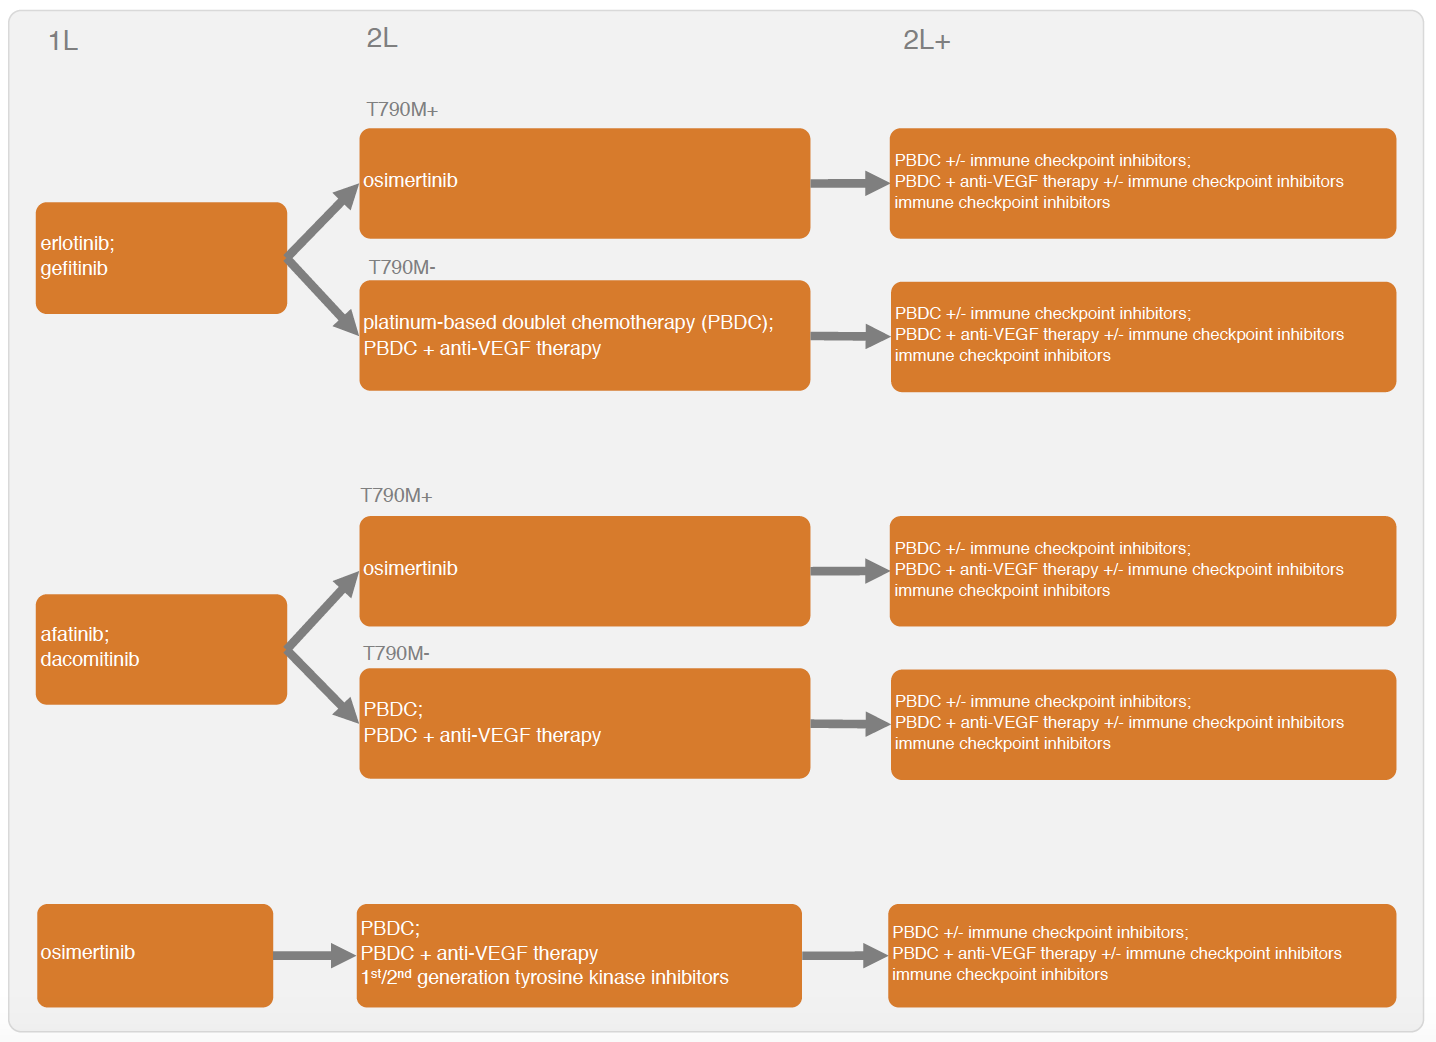
\includegraphics[max size={\textwidth}{\textheight}]{figs/treatment-strategies.png} 
\caption{Sequential treatment strategies of interest to be compared with the model}\label{fig:treatment-strategies}
\end{figure}

Tyrosine kinase inhibitors (TKIs) can be used at 1L. If osimertinib is not selected as the 1L treatment, then possible second line treatments (2L) and treatments beyond second line (2L+) depend on whether a patient acquired a T790M mutation. For example, after discontinuation of erlotinib, patients with a T790M mutation are treated with osimertinib while patients without a mutation can either be treated with platinum-based doublet chemotherapy (PBDC) or a combination of PBDC and anti-VEGF therapy. At 2L+, patients can be treated with a number of combination therapies including those that include immune checkpoint inhibitors (ICIs). Patients cannot be treated with the same treatment at multiple lines. 

The specific treatments included in the model are:

\begin{itemize}
\item \textbf{TKIs}: erlotinib, gefitinib, afatinib, dacomitinib, osimertinib
\item \textbf{anti-VEGF therapy}: bevacizumab
\item \textbf{ICIs}: nivolumab, pembrolizumab, atezolizumab

\end{itemize} 

\section{Model structure}\label{sec:model-structure}
\subsection{Disease model}
The IVI-NSCLC is an individual-level continuous-time state transition model (CTSTM) in which patients progress through multiple health states. Sequential treatment is modeled using the CTSTM by expanding the number of health states according to the number of treatment lines. In general, we define a health state for each treatment line, a health state after progression on the final line, and a death state, so a model with $n$ treatment lines will have $n+2$ health states. A patient with stable disease moves to the second treatment in a sequence after progression on the first treatment, to the third treatment after progression on the second treatment, and so on. A patient can die at any time. 

Unfortunately, the evidence base is currently too limited to explicitly model the transition rates by line of treatment and a simplified model structure is needed. Two options are available with the IVI-NSCLC model: a 4-state model (\autoref{fig:model-structure-4-states}) and a three-state model (\autoref{fig:model-structure-3-states}). The 3-state model is consistent with common methods for health economic modeling in oncology. In contrast, the 4-state model incorporates sequential treatment by explicitly modeling the effect of 2L treatment.  

In the 4-state model, patients begin 1L treatment in stable disease (S1) and can either transition to the progression state (P1) or death (D). At progression, patients move to the progression-free (stable) state (S2) with 2L treatment and can again either have their disease progress (P3) or die. At P3, patients begin 2L+ treatment and remain in the progressed state until death. Time-varying hazard rates for transitions between states $r$ and $s$ and are denoted by $h^{rs}(u)$.

\begin{figure}
\centering
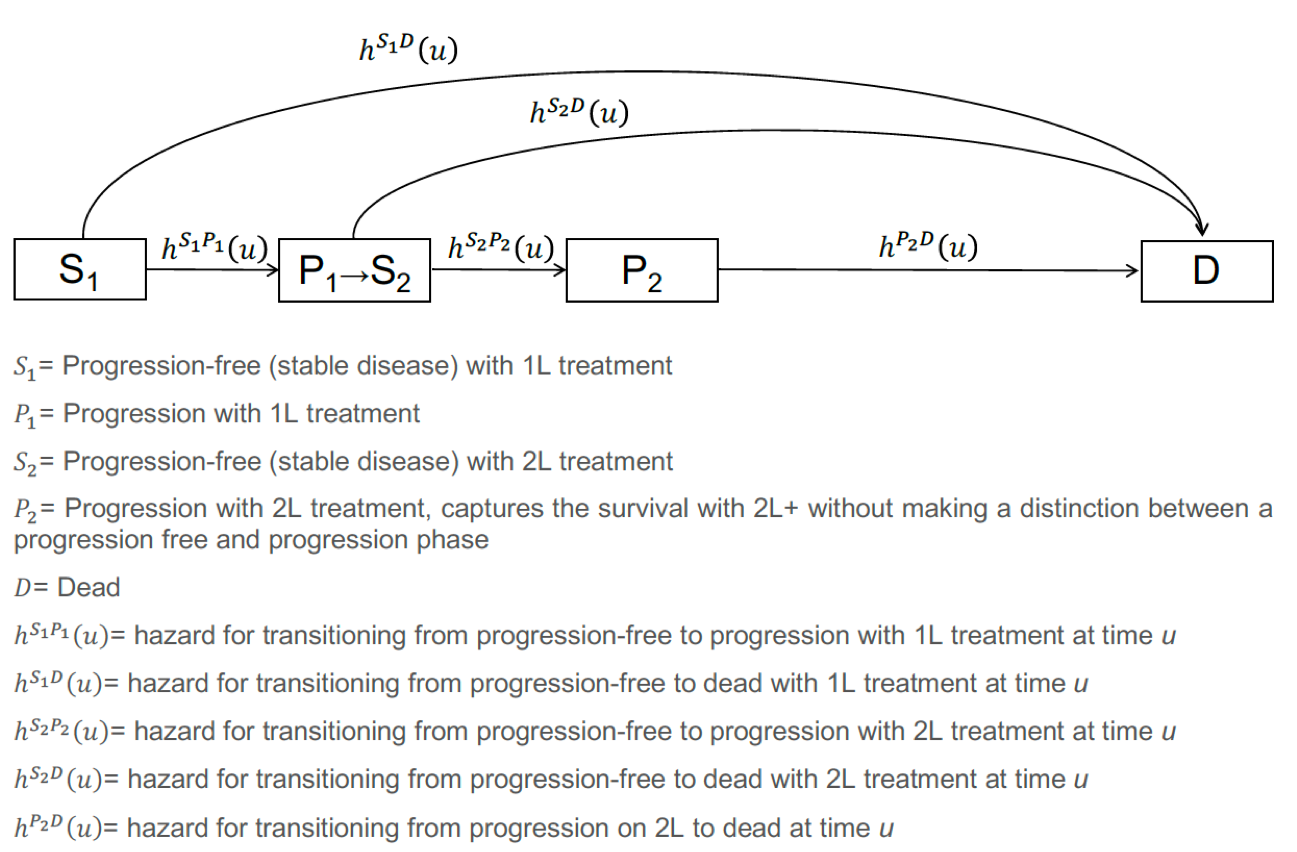
\includegraphics[scale = .7]{figs/model-structure-4-states.png}
\caption{Model structure with 4 states describing development of disease over time for a sequence starting with 1L, followed by 2L and 2L+ treatment; 2L+ treatment is captured with the L2 progression state}\label{fig:model-structure-4-states}
\end{figure}

In the three-state model, all hazard rates are based on 1L clinical trial evidence. Patients begin in stable disease (S1) and they can transition to the progression state (P1) or death (D).

\begin{figure}
\centering
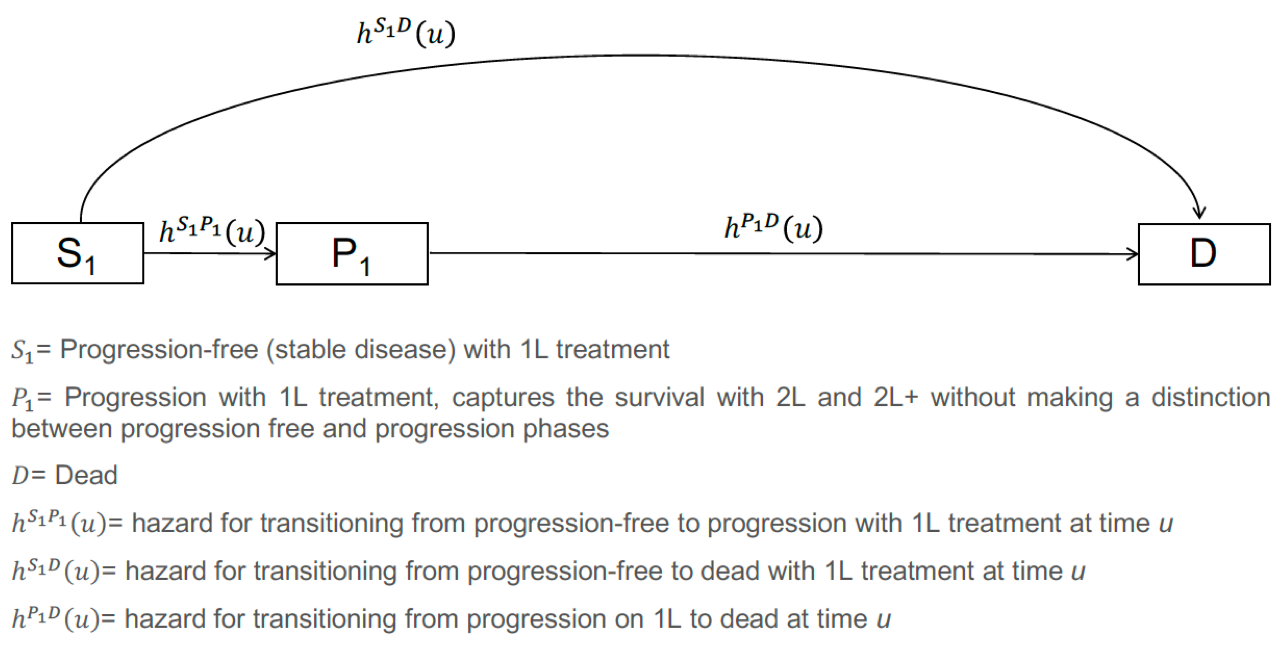
\includegraphics[scale = .7]{figs/model-structure-3-states.png}
\caption{Alternative model structure with 3 states describing development of disease over time for a treatment sequence starting with 1L until death; 2L and 2L+ treatment is captured with the progression state}\label{fig:model-structure-3-states} 
\end{figure}

The hazard rate, $h^{rs}(u)$, follows different parametric distributions as estimated with a multi-state network meta-analysis (NMA) for non-reversible 3-state models (\autoref{subsec:data-trans-rates}). As such, the disease model is perfectly integrated with the parameter estimation and the simulation techniques  depend on the statistical approach. In general, there are two type of multi-state models: "clock forward" (i.e., Markov) models and "clock reset" (i.e., semi-Markov) models. In the "clock reset" approach, time \textit{u} in $h^{rs}(u)$ resets to 0 after each transition whereas in the "clock forward" approach, time \textit{u} refers to time since the start of the model. If a "clock forward" approach is used, then health state probabilities can be calculated analytically using the \citet{aalen1978empirical} estimator; conversely, if a "clock reset" approach is taken, then individual-level simulation-based approaches must typically be used to estimate health state probabilities \citep{putter2007tutorial, de2011mstate, jackson2016flexsurv}. 

When a 3-state economic model is used, the 1L NMA is used to directly simulate disease progression and a "clock forward" approach is sufficient. However, if the number of health states is greater than $3$, then separate "clock forward" NMAs are fit to estimate line-specific transition rates. For example, in the 4-state model, the 1L results are used to simulate the transition from $S_1$ to $P_1 \rightarrow S_2$ and $S_1$ to $D$, and the 2L results are used to simulate the transition from $P_1 \rightarrow S_2$ to $P_2$, $P_2$ to $D$, and $P_1 \rightarrow S_2$ to $D$. In other words, in the 4-state model, a "clock forward" model is used for 1L but time \textit{u} resets when the patient begins 2L treatment. To accommodate this, we developed a new individual-level simulation approach that accommodates mixtures of "clock reset" and "clock forward" approaches (see \autoref{sec:uncertainty-analysis}).

Our statistical approach for modeling transitions between health states also allows us to incorporate potentially relevant prognostic factors or effect-modifiers, although we currently lack the individual-level data needed to do this. That is, we model the parameters of the survival distributions as functions of covariates so that they can vary across individuals and treatments. A given parameter, $\ a_{jt} $, for individual \textit{j} using treatment \textit{t} is modeled as $ \alpha_{jt} $ = $ \textit{g}^{-1} (X_{jt}\beta) $ where $ \textit{g}^{-1} $ (.) is an inverse transformation function. When data becomes available, this approach has a number of potential benefits including estimating health outcomes that are more precisely tailored to a subpopulation and including carry-over effects from one line of treatment to the next.


\FloatBarrier

\subsection{Adverse events}
The model simulates the probability of a number of distinct adverse events. Since the trials typically only report the number of proportion of patients experiencing an adverse event we were unable to model adverse events as a function of time on treatment and instead assume that adverse events occur during the first month of treatment as a function of the 1L treatment.

\subsection{Utility and health care sector costs}
Utility depends on the health state and the probability of an adverse event. Adverse events occur during the first month and cause utility decrements, which vary across treatments. After the first month, utility is only a function of the health state. 

Health care sector costs include treatment costs (i.e., drug acquisition and administration costs), costs due to inpatient hospitalizations, outpatient costs, and adverse event costs. Inpatient and outpatient costs vary by health state and accrue until death. Adverse event costs---which accrue during the first month---are a weighted sum of the probability of each adverse event and the event's expected cost. Treatment costs at a given line in the sequence accrue until until disease progression or, if dosage depends on time, the duration of the treatment.

\subsection{Productivity}
Productivity costs are currently estimated using the human capital approach (HCA), which measures lost productivity using work time lost. The approach is rooted in economic theory as time away from work is valued at the market wage, which, in a competitive market, reflects the societal value of work. The HCA contrasts with the friction cost approach (FCA), which only measures productivity costs during the time (i.e., the friction period) required to replace workers leaving employment due to illness. A practical limitation of the FCA is that it is difficult to reliably estimate the friction period, which depends on the unemployment rate and consequently varies considerably across individuals and over time. In general, the HCA tends to overestimate productivity costs while the FCA may underestimate them. 

Similar to \citet{hanly2012breast}, time lost from work in the model stems from three sources: temporary disability, permanent disability, and premature death. At cancer onset, patients miss days from work due to temporary disability which reflects work absence due to sick leave. Following sick leave, permanent survivors can then miss additional time from work due to permanent disability. Time lost due to premature death is the difference between the simulated age of death and the retirement age (age 65). Productivity costs are computed by valuing time lost from work at the market wage. 


\section{Model outcomes}\label{sec:model-outcomes}
The model simulates the health outcomes, adverse events, and costs associated with treatment strategies based on \autoref{fig:treatment-strategies}, which are combined for value assessment. The model's time horizon can be selected by the user and defaults to a lifetime horizon. The model outcomes are listed in \autoref{tbl:model-outcomes}.

\begin{table}[!ht]
\begin{center}
\begin{threeparttable}
\caption{Model outcomes} \label{tbl:model-outcomes}
\begin{tabular*}{\linewidth}{@{\extracolsep{\fill}}p{0.3\linewidth}p{0.60\linewidth}}
\hline
\multicolumn{1}{l}{Category} & \multicolumn{1}{l}{Outcomes}\\
\hline
Health outcomes & Health state probabilities; progression free survival \& overall survival; quality-adjusted life-years\\
&\\
Adverse events & Diarrhea, dry skin, elevated alanine transaminase, elevated aspartate transaminase, eye problems, paronychia, pneumonitis, pruritus, rash, stomatitis)\\
&\\
Health care sector costs & Drug acquisition and administration costs; adverse event costs; costs from inpatient hospital stays; costs from hospital outpatient or doctor office visits\\
&\\
Non-health care sector costs & Productivity costs \\
&\\
Value assessment & Cost-effectiveness analysis; multi-criteria decision analysis\\
\hline
\end{tabular*}
\scriptsize
\end{threeparttable}
\end{center}
\end{table}

\subsection{Health outcomes, adverse events, and costs}
The disease model simulates the times that patients transition to and from health states, which, in turn, is used to estimate the probability that a patient is in a given health state at a given point in time following treatment initiation. Progression free survival (PFS) with 1L treatment is defined as time in state $S_1$ while PFS with 2L is defined as time in state $P_1 \rightarrow S_2$. Overall survival is time until death. Adverse events are summarized using the probability of occurrence.  

Costs are computed for multiple categories and separated into health care sector and non-heath care sector costs as recommended by \citet{sanders2016recommendations}. Health care sector costs include treatment costs (i.e., drug acquisition and administration costs), adverse event costs, the costs of inpatient hospital stays, and costs from hospital outpatient and doctor office visits. Non-health care sector costs include productivity costs.

Discounted costs and QALYs over the model's time horizon are computed using the continuous time present value given a flow of state values (i.e., utility and annualized costs), which change as patients transition between health states or as costs vary as a function of time since treatment initiation. The state values can be partitioned into $M$ time intervals indexed by $m = 1,\ldots, M$ where interval $m$ contains times $u$ such that $u_m\leq u \leq u_{m+1}$ and state values are equal to $z_m$ during interval $m$. Discounted costs and QALYs are then given by,  

\begin{equation} \label{eqn:pv}
\sum_{m = 1}^M \int_{u_m}^{u_m+1} z_me^{-ru}du = \sum_{m = 1}^M z_m \left(\frac{e^{-r{u_{m}}} - e^{-r{u_{m+1}}}}{r}\right),
\end{equation}

where $r > 0$ is the discount rate. If $r = 0$, then the present value simplifies to $\sum_{m = 1}^M z_m(u_{m+1} - u_{m})$. 

\subsection{Value assessment} \label{subsec:outcomes-value-assessment}
If CEA is used for value assessment, then the value of treatment is estimated using the NMB defined as discounted QALYs multiplied by willingness to pay per QALY less costs. Costs in analyses conducted from a limited societal perspective include both productivity costs and health care sector costs while costs in analyses conducted from a health care sector perspective only include health care sector costs. 

Any combination of simulated model outcomes can be used for MCDA. If a 3-state model is selected, the MCDA in IVI's web applications is currently based on the following criteria: progression free survival (PFS) with 1L treatment, post-progression survival, total health care sector costs,oral administration (vs. intravenous administration), and years since FDA approval. If a 4-state model is selected, then PFS with 2L treatment is added as an additional criteria. Similarly, if the MCDA is conducted from limited societal perspective, then productivity costs are added as a criteria. Performance on the oral administration criteria is computed as the percentage of simulated life-years treated using oral therapies rather than intravenous therapies. Performance on the years since FDA approval criteria is the weighted time since FDA approval for each treatment in a treatment sequence, with weights equal to the number of life-years spent using a particular treatment with the sequence. In the web interfaces users can input their own weights for each of the criteria, but it is important to note that we have not conducted the surveys required to elicit weights for a representative sample of patients.

\section{Source data and parameter estimation}\label{sec:data}
Key parameters for the model relate to: (i) treatment effects in terms of transitions between the health states; (ii) adverse events; (iii) utilities; (iv) healthcare resource use; and (v) productivity. Parameter estimates for the current version of the IVI-NSCLC(egfr+) model are based on currently available published evidence identified by means of a systematic literature review and synthesized with meta-analysis techniques where appropriate. To inform relevant decision-making at the local level, it is recommended to use resource use and cost estimates reflective of that setting. 

\subsection{Treatment effects for transition rates} \label{subsec:data-trans-rates}
Relevant evidence to estimate treatment effects with the alternative TKIs and chemotherapy regimens in terms of transitions between the health states was obtained with a systematic literature review of RCTs evaluating the efficacy of relevant competing interventions for the treatment of adult patients with metastatic EGFR+ non-squamous NSCLC by line of treatment (i.e. 1L, 2L, and 2L+) in terms of OS and PFS. Details regarding eligibility criteria, included studies, extracted information regarding study, treatment, and patient characteristics, and Kaplan-Meier survival curves are provided in \autoref{app:km-curves}. 
The identified evidence base was used to 1) estimate the relative treatment effects for each 1L treatment versus a defined reference treatment; 2) estimate the absolute effects with the corresponding 1L reference treatment; and 3) estimate the absolute treatment effects with 2L treatment options. 

It is important to note that the available PFS and OS data for the different interventions varied dramatically. At the time when the systematic literature review was performed, there was about 25 months of follow-up data available for osimertinib as 1L treatment, with median OS not yet reached; about 40 months of data for dacomitinib; 40-50 months for afatinib; and more than 50 months of follow-up data for gefitinib and erlotinib. This implies that treatment effect estimates for osimertinib and dacomitinib are much more uncertain than the other interventions at this stage, and are likely to change when longer term data become available. See \autoref{fig:FLAURA}-\autoref{fig:Yang 2014} for more detail.

\subsubsection{Relative treatment effects with 1L therapy}
Relative treatment effects of the competing TKIs in comparison to gefitinib for the 1L treatment of EGFR+ NSCLC were estimated by means of a Bayesian network meta-analysis (NMA) using alternative fixed and random effects models. 

RCTs are considered the gold standard to assess treatment effects of medical interventions. For many disease states there are multiple competing interventions to choose from. However, an RCT will rarely include all competing interventions of interest for a particular disease state when there are more than two relevant treatment options available. As such, an individual trial rarely provides all the information needed to guide evidence-based treatment selection. When each RCT compares only a subset of the interventions of interest---it may be possible to represent the evidence base as a network where all trials have at least one intervention in common with another trial. Such a network of trials involving treatments compared directly, indirectly, or both, can be synthesized by means of a network meta-analysis \citep[Chapter~1]{dias2018network}.. As a result we not only get pooled results of available treatment comparisons studied in a head-to-head fashion but also relative treatment effects between interventions not compared directly. In order to ensure that a network meta-analysis are not affected by bias due to differences in prognostic factors between studies, we want to only consider the relative treatment effects of each trial. This implies that all interventions have to be part of one network of trials where each trial has at least one intervention in common with another trial.  

Patients are randomized only within trials, not across trials, so there is a risk that patients participating in different trials differ with respect to demographic, disease or other characteristics. In addition, features of the trials themselves may differ. If these trial or patient characteristics are effect modifiers, i.e. they affect the treatment effects of an intervention versus a control, then there are systematic differences in treatment effects across trials. Systematic differences in known and unknown effect-modifiers among studies comparing the same interventions in direct fashion result in between-study heterogeneity. An imbalance in the distribution of effect modifiers between studies comparing different interventions will result in transitivity or consistency violations and therefore biased indirect comparisons.

The RCTs that were part of one evidence network and were deemed sufficiently similar were included in the NMA. The evidence network for 1L treatments is presented in \autoref{fig:RCT network-1L}. Information regarding the distribution of patients characteristics across the studies in the network  are presented in \ \autoref{app:patient-characteristics}. 

\begin{figure}
\centering
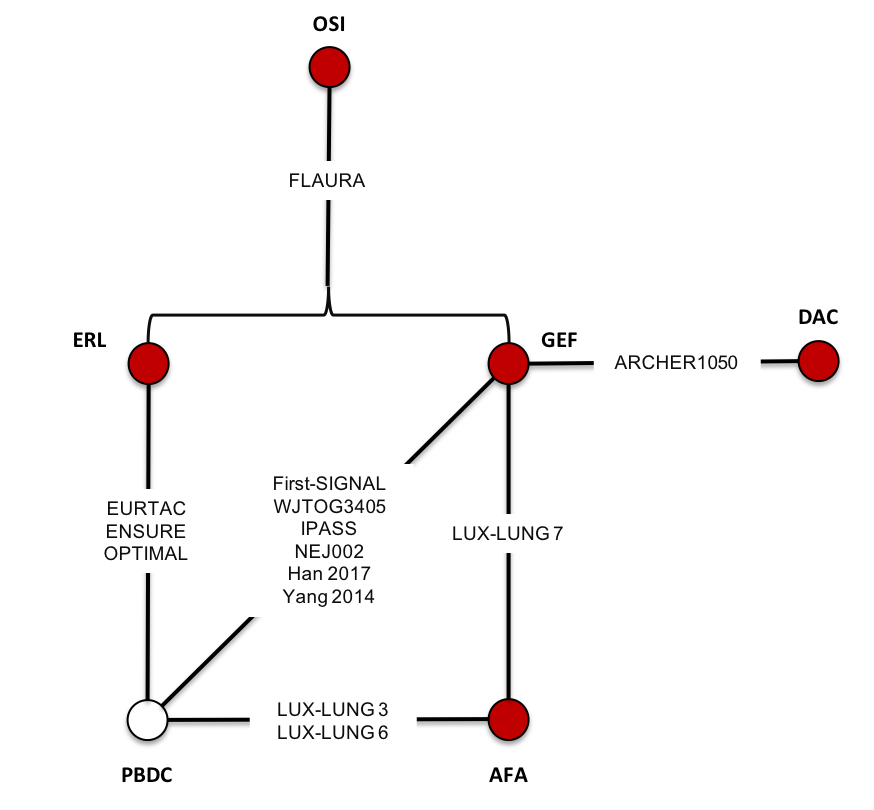
\includegraphics[max size={\textwidth}{\textheight}]{figs/RCT-network-1L.png}
\caption{Network of RCTs to estimate relative treatment effects regarding PFS and OS with 1L therapies}\label{fig:RCT network-1L}
\end{figure}

\FloatBarrier

\subsubsubsection{Network meta-analysis model}
Traditionally, NMAs in oncology are based on separate analyses for OS and PFS, with relative treatment effects estimated using reported hazard ratios (HR). There are two limitations of this approach. First, HR estimates rely on the proportional hazard assumption, which is implausible if the hazard functions of the competing interventions cross \citep{dias2018network}. Second, separate analyses of OS and PFS ignore the structural relationship between stable disease, progression, and death and implicitly assume that transition probabilities for stable to death and progression to death are equal.

We overcome these limitations by introducing a multi-state NMA that explicitly estimates each possible transition in a 3-state model---stable to progression, stable to death, and progression to death--and modeling time-varying hazard rates and relative treatment effects with known parametric survival functions or fractional polynomials. Our approach is illustrated in \autoref{fig:multistate-nma} and expressed mathematically as follows:

\FloatBarrier


\begin{figure}
\centering

\includegraphics[max size={\textwidth}{\textheight}]{figs/multistate-nma.png}
\caption{Relationship between stable disease (S), progression (P) and death (D) as used in the multi-state network meta-analysis model}\label{fig:multistate-nma}
\end{figure}



\begin{equation}\label{eqn:multistate-nma}
\begin{aligned} 
% SP transition
\ln\left(h_{ik}^{SP}(u)\right) &= 
\begin{cases}
\alpha_{1ik} + \alpha_{2ik}u^{p_1} + \alpha_{3ik}u^{p_2} & \text{if } p_1 \neq p_2 \\ 
\alpha_{1ik} + \alpha_{2ik}u^{p} + \alpha_{3ik}u^{p}\ln(u) & \text{if } p_1 = p_2 = p \\ 
\end{cases}\\ 
% SD transition 
\ln\left(h_{ik}^{SD}(u)\right) &=
\alpha_{4ik}\\
% PD transition
\ln\left(h_{ik}^{PD}(u)\right) &=
\alpha_{5ik} + \alpha_{6ik}u^{p_1}\\ 
\\
% Coefficient matrix
\begin{pmatrix}
\alpha_{1ik} \\
\alpha_{2ik} \\
\alpha_{3ik} \\
\alpha_{4ik} \\
\alpha_{5ik} \\
\alpha_{6ik} \\
\end{pmatrix}
&= 
\begin{pmatrix}
\mu_{1ik} \\
\mu_{2ik} \\
\mu_{3ik} \\
\mu_{4ik} \\
\mu_{5ik} \\
\mu_{6ik} \\
\end{pmatrix} 
+
\begin{pmatrix}
\delta_{1,ik} \\
d_{2, t_{ik}} - d_{2, t_{i1}}  \\
0 \\
0  \\
d_{3, t_{ik}} - d_{3, t_{i1}} \\
0 \\
\end{pmatrix} \\\\ 
% Random effects
\delta_{1,ik} &\sim N(d_{1, t_{ik}} - d_{1, t_{i1}}, \sigma_{d_{1}}^{2}) 
\end{aligned}
\end{equation}

where $u^0= \ln(u)$ and ${d_{1,1}}=0$, ${d_{2,1}}=0$, and ${d_{3,1}}=0$
\\

$h_{ik}^{SD}(u)$, $h_{ik}^{PD}(u)$, and $h_{ik}^{SD}(u)$ are the the hazard rate for disease progression, dying post-progression, and dying pre-progression, respectively, in study $i$ for treatment arm $k$ at time $u$. The $\alpha_{\cdot ik}$ are regression coefficients that represent the scale and shape parameters of the log hazard function in study $i$ for treatment arm $k$. The $\mu_{\cdot i}$ reflect the study effects regarding the scale and shape parameters in each study $i$. The $\delta_{1,ik} $ are the study specific true underlying relative treatment effects regarding the scale of the log hazard function for the transition from stable to progression, which are described by a normal distribution with an average effect for treatment $t$ relative to reference treatment 1, ${d_{1,1t}}$, and between study heterogeneity $\sigma_{d_{1}}^{2} $.  ${d_{2,1t}}$ are the treatment specific relative effects regarding the first shape parameter of the log hazard function for the transition from stable to progression relative to the reference treatment 1 (i.e. gefitinib). To facilitate parameter estimation, we assumed that treatment has no effect on the 2nd shape parameter. Transition rates between stable disease and death are likely to be relatively small and therefore assumed to be independent of time and the same for all treatments. ${d_{3,1t}}$ are the treatment specific relative effects regarding the scale parameter of the log-hazard function for the transition from progression to death relative to reference treatment 1 (i.e. gefitinib). 

When $p_{1}=0$ and $\alpha_{3ik}=0$ the log-hazard functions for the transitions between stable disease and progression, and progression and death follow a Weibull distribution. When $p_{1}=1$ and $\alpha_{3ik}=0$ these log-hazard functions follow a Gompertz distribution. When $\{(p_1, p_2) = (0, 0), (0,1)\}$ and $\alpha_{3ik}\neq0$, the log-hazard functions follow a second order fractional polynomial that are extensions of the Weibull and Gompertz model to allow for arc- and bathtub shaped log-hazard functions. 

A fixed effects model is obtained by replacing $\delta_{1,ik} \sim N(d_{1, t_{ik}} - d_{1, t_{i1}}, \sigma^2)$ with $\delta_{1,ik} = d_{1, t_{ik}} - d_{1, t_{i1}}$. 

If it is assumed that treatment has only a direct effect on the transitions from stable to progression, which can be reasonably defended when a particular treatment upon disease progression is discontinued, the model can be simplified by setting $d_{3, t_{i1}}=0$.


\subsubsubsection{Likelihood}
The model parameters were estimated based on the number of patients $r$ in each of the three health states (stable, progression and death) at time $u$ for each arm $k$ of each trial $i$ obtained from the published Kaplan-Meier (KM) curves for time points for which both PFS and OS were reported. Accordingly, a multinomial likelihood was used for the proportion of patients in each of the three health states at any time point for each arm of each trial ($S_{ik}(u)$, $P_{ik}(u)$, and $D_{ik}(u)$) according to: 

\begin{equation} \label{eqn:multinomial_likelihood}
\begin{aligned}
% Likelihood
(r_{ik}^{S}(u),r_{ik}^{P}(u),r_{ik}^{D}(u)) \sim multinomial(S_{ik}(u),P_{ik}(u),D_{ik}(u),n_{ik}(u))
\end{aligned}
\end{equation}

where $n_{ik}(u)=r_{ik}^{S}(u)+r_{ik}^{P}(u)+r_{ik}^{D}(u)$ and $S_{ik}(u)+P_{ik}(u)+D_{ik}(u)=1$
\\

Arbitrary hazard rate functions can be approximated with a set of discontinuous constant hazard rates over successive time intervals. The total follow-up time can be partitioned into $M$ successive non-overlapping intervals indexed by $m= 1, ..., M$. We refer to interval $m$ as $U_{m}$ and write $u \in U_{m}$ to denote $u_{m}\leq u<  u_{m+1}$. The length of $U_{m}$ is $\Delta u_{m} =u_{m+1}-u_{m}$. 

For each interval $m$, the proportions  $S_{ik}(u)$, $P_{ik}(u)$, and $D_{ik}(u)$ are related to the time-varying hazards $\ h_{ik}^{SP} (u) $,$\ h_{ik}^{SD} (u) $, $\ h_{ik}^{PD} (u)$ according to the following set of differential equations \citep{jansen2013multivariate}: 

\begin{equation} \label{eqn:diff_equations}
\begin{aligned}
% Differential equations
S_{ik}(u) &= S_{ik}(u_{m}) e^{-(h_{ikm}^{SP}+h_{ikm}^{SD})(u-u_{m})} \\
P_{ik}(u) &= P_{ik}(u_{m}) e^{-h_{ikm}^{PD}(u-u_{m})}+\frac{S(u_{m})h_{ikm}^{SP}(e^{-(h_{ikm}^{SP}+h_{ikm}^{SD})(u-u_{m})}-e^{-h_{ikm}^{PD}(u-u_{m})})}{h_{ikm}^{PD}-h_{ik}^{SP}-h_{ikm}^{SD}} \\
D_{ik}(u) &= 1-S_{ik}(u) - P_{ik}(u) \\
\end{aligned}
\end{equation}
\\

In order to estimate $h_{ikm}^{SP}$, $h_{ikm}^{SD}$, and $h_{ikm}^{PD}$ for each interval $m$,  data at three time points were used: $u_{m}$, $u_{m+\frac{1}{2}}$, and $u_{m+1}$. The obtained estimates of the hazards for interval $m$ were assigned to the time point corresponding to the mid point of the interval when used in the NMA.
\\

For time points of a trial for which only OS data was reported (and no PFS data was available anymore), the number of patients that survived time interval $m$ ($r_{ikm}^{OS}$) out of the number of patients alive at the beginning of interval ($n_{ikm}^{OS}$) were used for the model parameter estimation. A binomial likelihood was used for the conditional survival probabilities ($p_{ikm}^{OS}$):


\begin{equation} \label{eqn:binomial_likelihood}
\begin{aligned}
% Likelihood
r_{ikm}^{OS} \sim binomial(p_{ikm}^{OS},n_{ikm}^{OS})
\end{aligned}
\end{equation}
\\
Given the generally small estimate for $h^{SD}$, the conditional survival probabilities were assumed to inform $h_{ik}^{SD}(u)$ and $h_{ik}^{PD}(u)$ at these time points according to:

\begin{equation} \label{eqn:diff_equations_OS}
\begin{aligned}
% Differential equations OS
p_{ikm}^{OS} &= e^{-(h_{ikm}^{SD}+h_{ikm}^{PD})(u-u_{m})} \\
\end{aligned}
\end{equation}
where the obtained estimates of the hazards for interval $m$ assigned to the time point corresponding to the mid point of the interval when used in the NMA.
\\

\subsubsubsection{Prior distributions}
The following prior distributions for the parameters of the model expressed with \autoref{eqn:multistate-nma} were used:

\begin{equation} \label{eqn:multistate-nma-priors}
\begin{aligned}
% Prior for mu's
\begin{pmatrix}
\mu_{1i}  \\
\mu_{2i}  \\
\mu_{3i}  \\
\mu_{4i}  \\
\mu_{5i}  \\
\mu_{6i}  \\
\end{pmatrix} 
&\sim 
MVN\left(
\begin{pmatrix}
0  \\
0  \\
0  \\
0  \\
0  \\
0 \\
\end{pmatrix}, 
T_\mu
\right) 
\qquad
T_\mu =
\begin{pmatrix}
100 & 0 & 0 & 0 & 0 & 0 \\
0 & 10 & 0 & 0 & 0 & 0 \\
0 & 0 & 10 & 0 & 0 & 0 \\
0 & 0 & 0 & 100 & 0 & 0 \\
0 & 0 & 0 & 0 & 100 & 0 \\
0 & 0 & 0 & 0 & 0 & 10 \\
\end{pmatrix}\\\\
%
% Prior for ds
\begin{pmatrix}
d_{1, 1t}  \\
d_{2, 1t}  \\
d_{3, 1t}  \\
\end{pmatrix} 
&\sim 
MVN\left(
\begin{pmatrix}
0  \\
0  \\
0 \\
\end{pmatrix}, 
T_d
\right) 
\qquad
T_d =
\begin{pmatrix}
2 & 0 & 0  \\
0 & 1 & 0   \\
0 & 0 & 2  \\
\end{pmatrix} \\
%
\\
% Prior for between-study heterogeneity
\sigma_{d_{1}} &= uniform(0, 2)  \\
\end{aligned}
\end{equation}

The prior distribution for the probabilities at the beginning of each interval, $u_{m}$ was: 

\begin{equation} \label{eqn:multinomial-prior}
\begin{aligned}
% Prior for probabilities at beginning of interval
(S_{ik}(u_{m}),P_{ik}(u_{m}),D_{ik}(u_{m})) \sim Dirichlet(0,0,0) \\
\end{aligned}
\end{equation}

\subsubsubsection{Estimated time-varying hazard ratios}
The time-varying HRs corresponding to the parameter estimates  ${d_{1,t}}$ and ${d_{2,t}}$   of the fixed effects Weibull, Gompertz, and fractional polynomial models without a treatment effect for progression to death (i.e. ${d_{3,t}=0}$) are presented in \autoref{fig:hr-1L} and \autoref{fig:hr-1L-weibull}- \autoref{fig:hr-1L-gompertz}.


\begin{figure}[h]
\centering
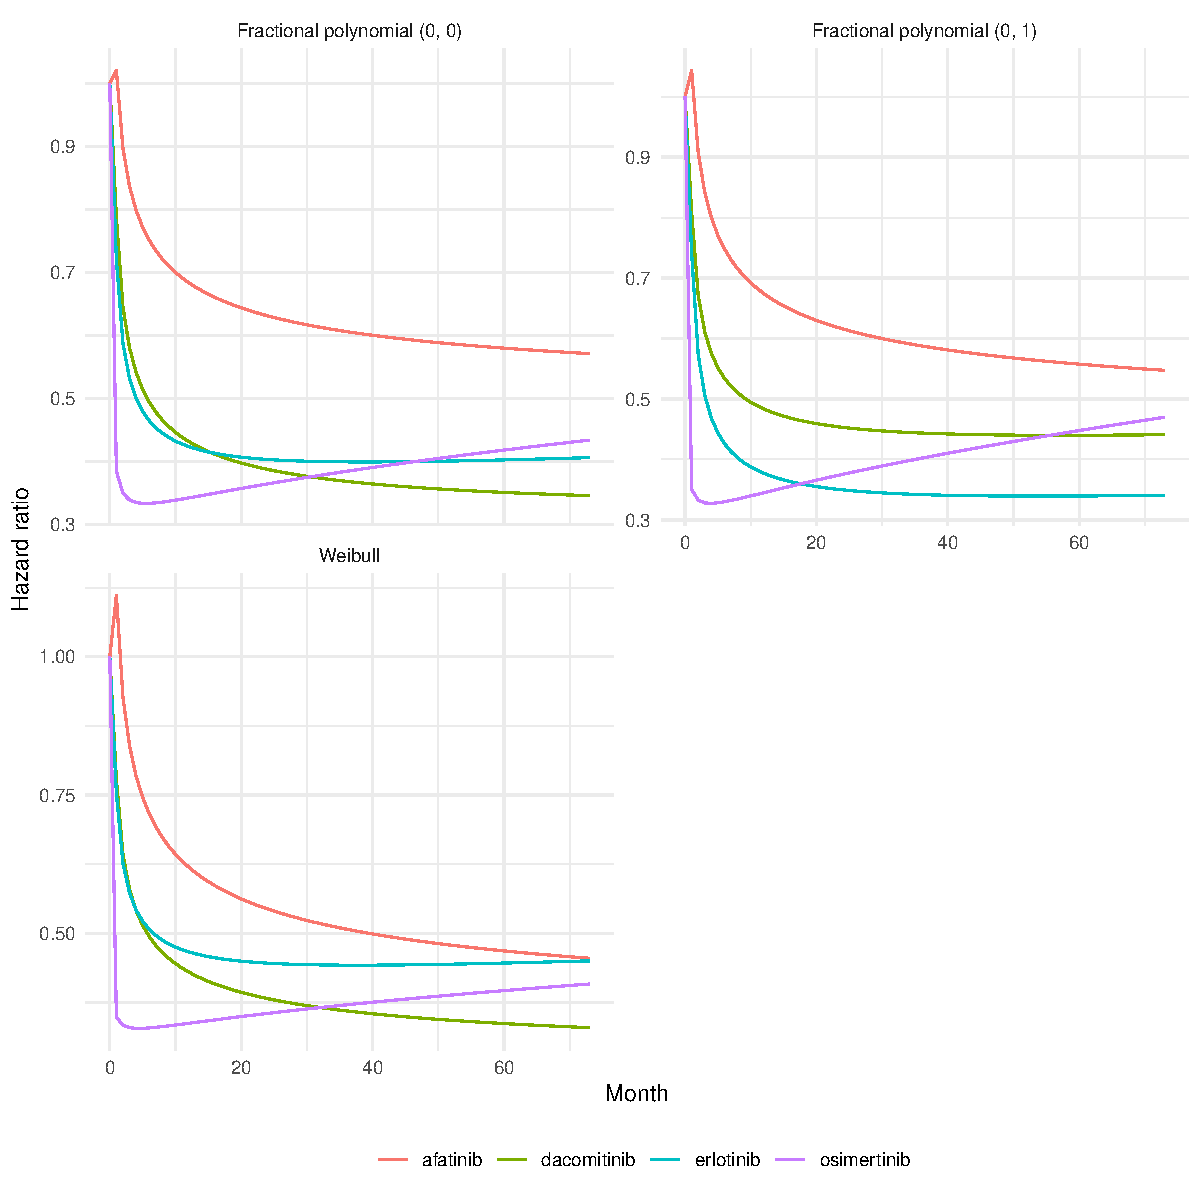
\includegraphics[max size={\textwidth}{\textheight}]{figs/hr-1L.pdf} 
\caption{First line estimates of hazard ratios from stable to progression relative to gefitinib from the multi-state network meta-analysis}\label{fig:hr-1L}
\end{figure}



\subsubsection{Absolute effects with 1L reference treatment}
Absolute effects with 1L therapy with the reference intervention, i.e. gefitinib, were estimated with the multi-state meta-analysis model expressed in \autoref{eqn:multistate-ma} with likelihoods and transformations according to \autoref{eqn:multinomial_likelihood}, \autoref{eqn:diff_equations}, \autoref{eqn:binomial_likelihood}, and \autoref{eqn:diff_equations_OS} based on the reported KM curves of all the gefitinib treatment arms of the available RCTs.

\begin{equation}\label{eqn:multistate-ma}
\begin{aligned} 
% SP transition
\ln\left(h_{i}^{SP}(u)\right) &= 
\begin{cases}
M_{1} + M_{2}u^{p_1} + M_{3}u^{p_2} & \text{if } p_1 \neq p_2 \\ 
M_{1} + M_{2}u^{p} + M_{3}u^{p}\ln(u) & \text{if } p_1 = p_2 = p \\ 
\end{cases}\\ 
% SD transition 
\ln\left(h_{i}^{SD}(u)\right) &=
M_{4}\\
% PD transition
\ln\left(h_{i}^{PD}(u)\right) &=
M_{5} + M_{6}u^{p_1}\\ 
\\
\end{aligned}
\end{equation}

where $u^0= \ln(u)$
\\

$h_{i}^{SD}(u)$, $h_{i}^{PD}(u)$, and $h_{i}^{SD}(u)$ are the underlying hazard rates for disease progression, dying post-progression, and dying pre-progression, respectively, in study $i$ at time $u$. The $M_{\cdot}$ represent the pooled scale and shape parameters describing the log hazard functions over time. As before, when $p_{1}=0$ and $M_{3}=0$ the log-hazard functions for the transitions between stable disease and progression, and progression and death follow a Weibull distribution. When $p_{1}=1$ and $M_{3}=0$ these log-hazard functions follow a Gompertz distribution. When $\{(p_1, p_2) = (0, 0), (0,1)\}$ and $M_{3}\neq0$, the log-hazard functions follow a second order fractional polynomial. The following prior distribution for the parameters of the model was used:

\begin{equation} \label{eqn:multistate-ma-priors-gef}
\begin{aligned}
% Prior for mu's
\begin{pmatrix}
M_{1}  \\
M_{2}  \\
M_{3}  \\
M_{4}  \\
M_{5}  \\
M_{6}  \\
\end{pmatrix} 
&\sim 
MVN\left(
\begin{pmatrix}
0  \\
0  \\
0  \\
0  \\
0  \\
0 \\
\end{pmatrix}, 
T_M
\right) 
\qquad
T_M =
\begin{pmatrix}
100 & 0 & 0 & 0 & 0 & 0 \\
0 & 10 & 0 & 0 & 0 & 0 \\
0 & 0 & 10 & 0 & 0 & 0 \\
0 & 0 & 0 & 100 & 0 & 0 \\
0 & 0 & 0 & 0 & 100 & 0 \\
0 & 0 & 0 & 0 & 0 & 10 \\
\end{pmatrix}\\\\
\end{aligned}
\end{equation}


\autoref{fig:hazard-gef-1L} and \autoref{fig:hazard-1L-gef-weibull} - \autoref{fig:hazard-1L-gef-gompertz} show the hazard functions for the transitions between stable, progression, and death with gefitinib for each fitted model.

The posterior distributions of $M_{\cdot}$ along with the parameters representing the relative treatment effects of each TKI relative to gefitinib ($d_{1, t}$ and ${d_{2,t}}$), were used to simulate a posterior distribution for PFS and OS as displayed in \autoref{fig:surv-1L} and \autoref{fig:surv-1L-weibull}- \autoref{fig:surv-1L-gompertz} for each 1L treatment and each fitted model. 


\begin{figure}[h]
\centering
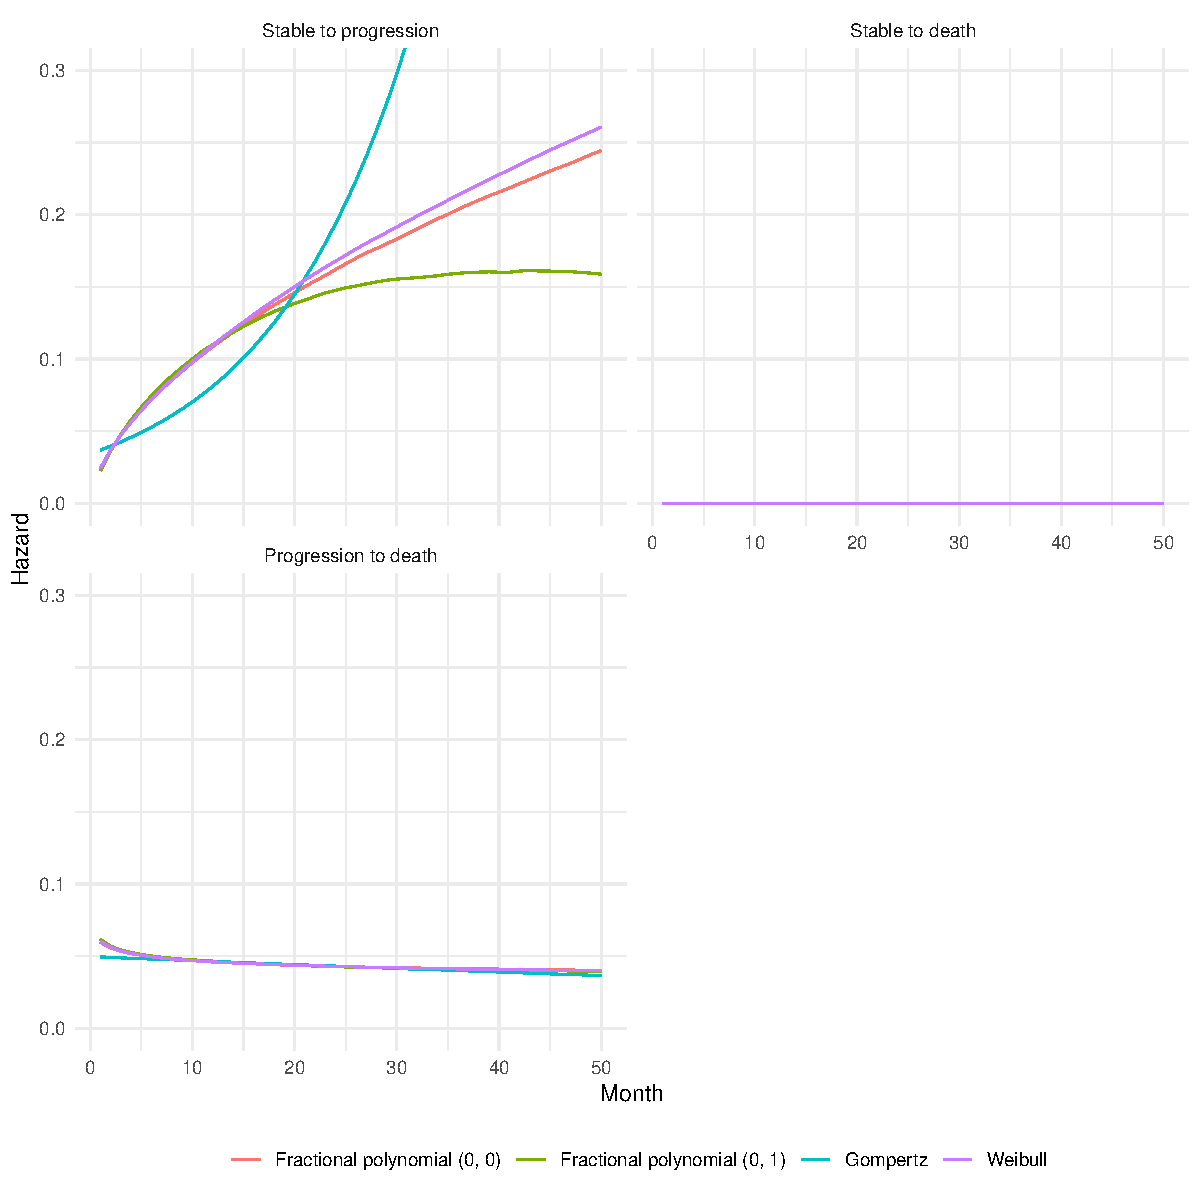
\includegraphics[max size={\textwidth}{\textheight}]{figs/hazard-1L-gef.pdf} 
\caption{First line estimates of hazard rates over time for transitions between S, P and D with gefitinib from the multi-state meta-analysis}\label{fig:hazard-gef-1L}
\end{figure}


\begin{figure}[h]
\centering
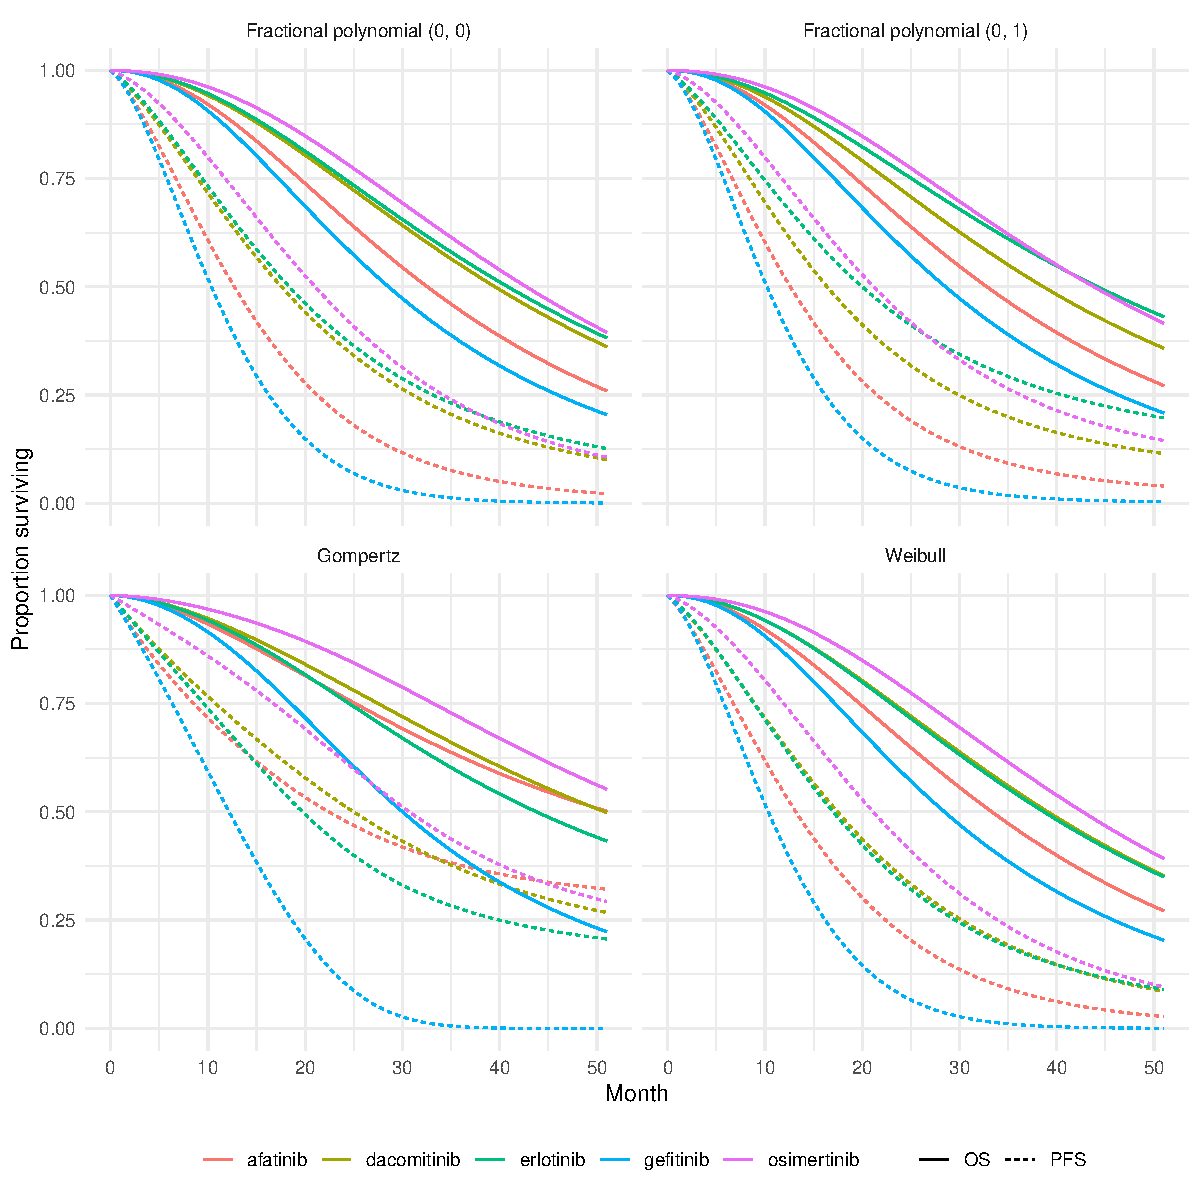
\includegraphics[max size={\textwidth}{\textheight}]{figs/surv-1L.pdf} 
\caption{First line estimates of progression-free survival and overall survival for the competing interventions obtained with the multi-state (network) meta-analysis}\label{fig:surv-1L}
\begin{minipage}{\linewidth}
\footnotesize
Notes: The simulated posterior distribution of the parameters of the Bayesian multi-state NMA was used to simulate a distribution of progression-free survival and overall survival curves. The curves in the figure are posterior means. Curves with credible intervals are shown in the appendix.
\end{minipage}
\end{figure}

\FloatBarrier


\subsubsection{Absolute effects with 2L therapy}
For the 2L treatment options, the available number of RCTs among patients who progressed on 1L TKI were limited. For T790M positive patients, the transition rates with osimertinib were estimated based on data from two RCTs according to \autoref{eqn:multistate-ma} and with a prior distribution according to \autoref{eqn:multistate-ma-priors-gef}. Regarding other possible treatments, there was only data available for PBDC from three RCTs, which were used to estimate transition rates according to \autoref{eqn:multistate-ma} and \autoref{eqn:multistate-ma-priors-gef} as well. In the absence of RCT evidence, these estimates were assumed to be representative of the other 2L treatment regimens presented in \autoref{fig:treatment-strategies} for both an all-comer population and a T790M mutation negative population. \autoref{fig:hazards-2L} and \autoref{fig:hazard-2L-weibull} -  \autoref{fig:hazard-2L-gompertz} show the hazard functions for the transitions between stable, progression, and death for each fitted model and \autoref{fig:surv-2L} show the corresponding PFS and OS curves.

\FloatBarrier



\begin{figure}
\centering
\begin{subfigure}{\textwidth}
\centering
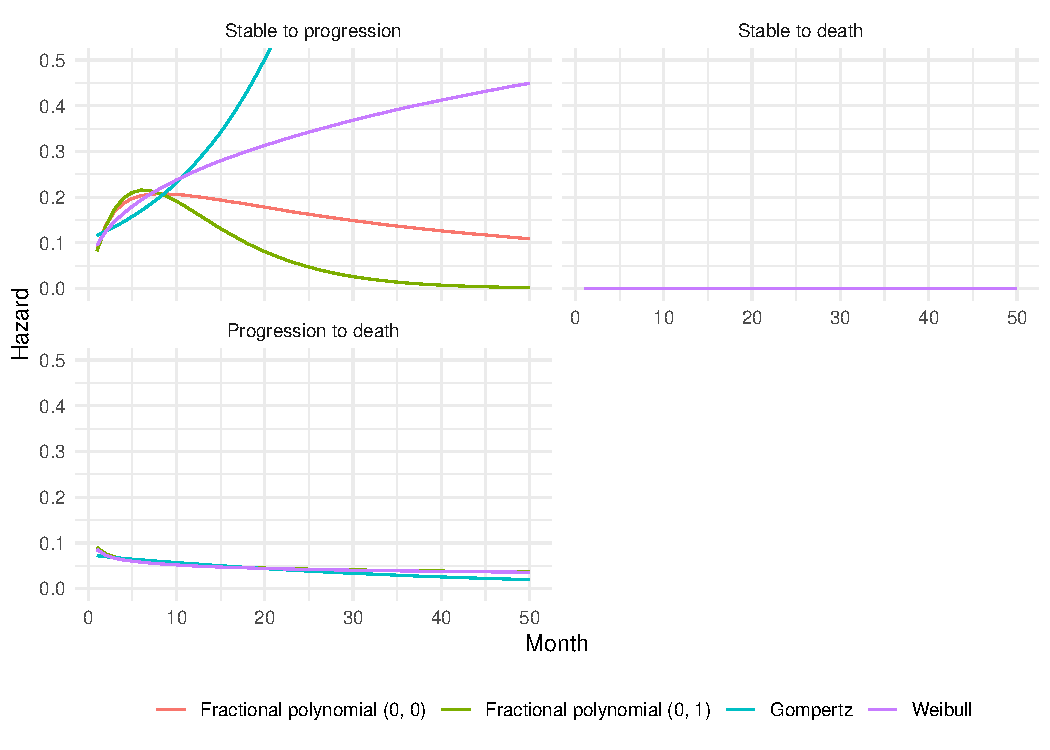
\includegraphics[max size={.8\textwidth}{.8\textheight}]{figs/hazard-2L-pbdc.pdf}
\caption{Platinum based doublet chemotherapy} \label{subfig:hazard-2L-pbdc}
\end{subfigure}
\begin{subfigure}{\textwidth}
\centering
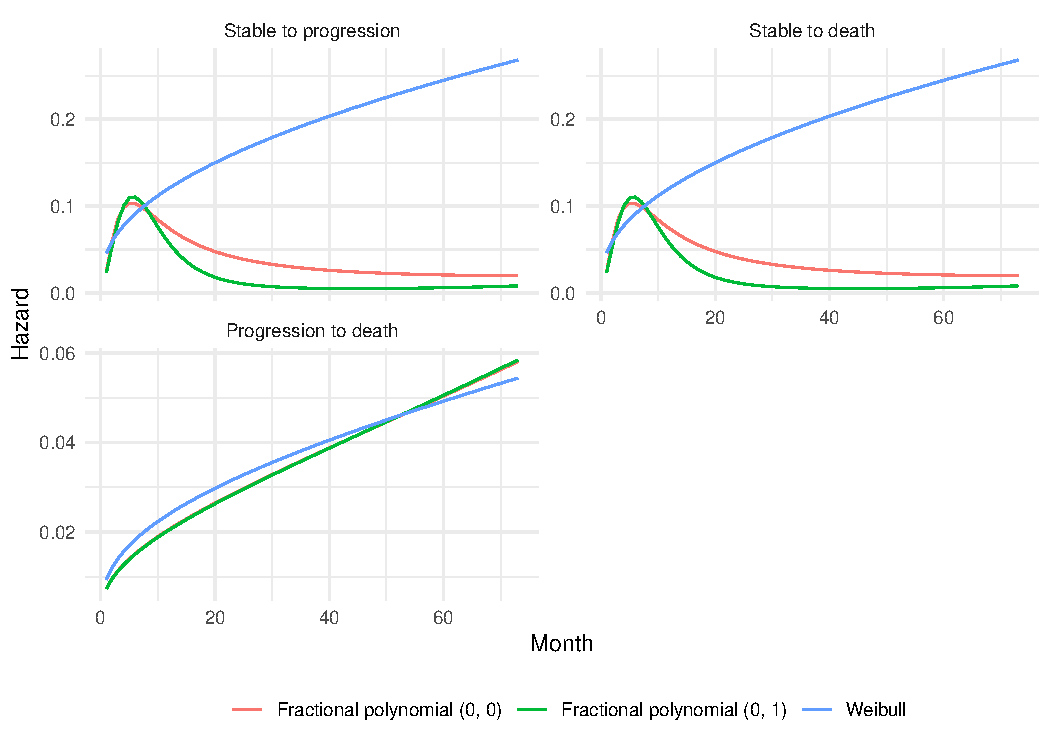
\includegraphics[max size={.8\textwidth}{.8\textheight}]{figs/hazard-2L-t790m-osi.pdf}
\caption{Osimertinib among T790M positive patients} \label{subfig:hazard-2L-t790m-osi}
\end{subfigure}
\caption{Second line estimates of hazard rates over time for transitions between S, P and D from the multi-state meta-analysis}\label{fig:hazards-2L}
\end{figure}




\begin{figure}
\centering
\begin{subfigure}{\textwidth}
\centering
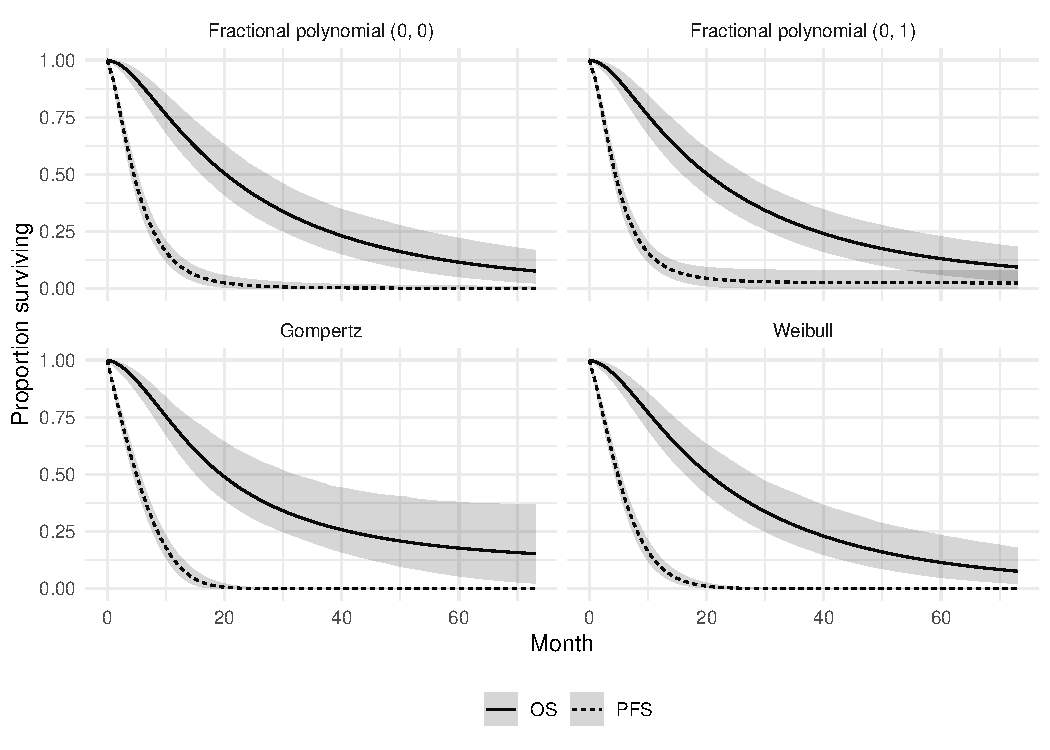
\includegraphics[max size={.8\textwidth}{.8\textheight}]{figs/surv-2L-pbdc.pdf}
\caption{Platinum based doublet chemotherapy} \label{subfig:surv-2L-pbdc}
\end{subfigure}
\begin{subfigure}{\textwidth}
\centering
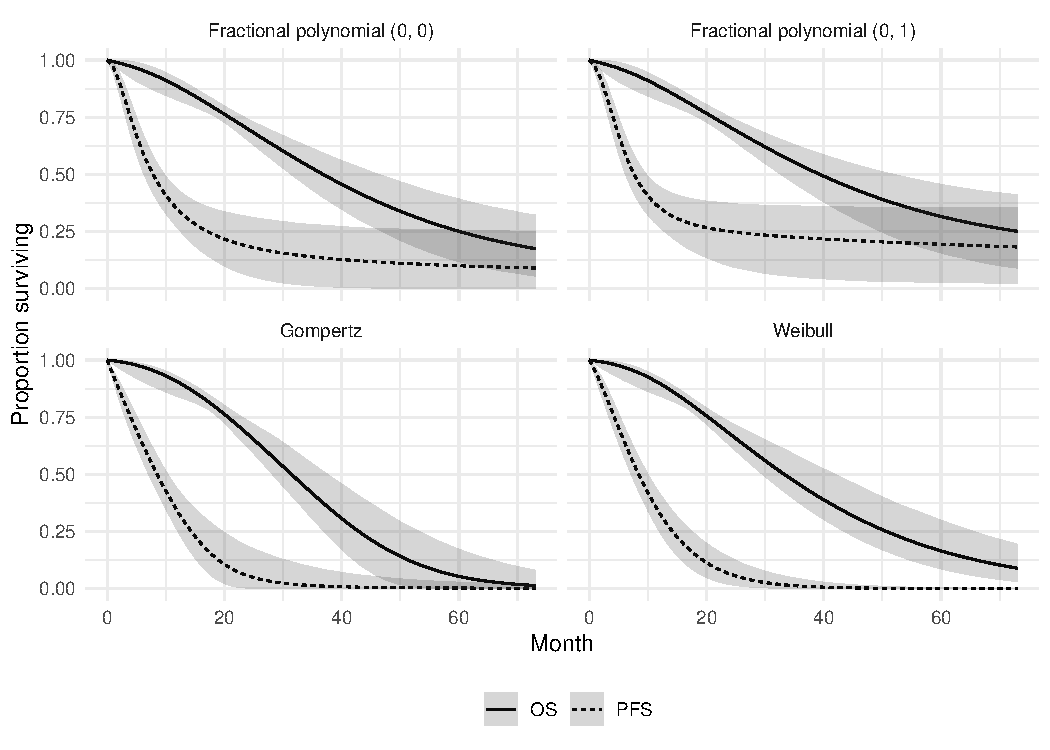
\includegraphics[max size={.8\textwidth}{.8\textheight}]{figs/surv-2L-t790m-osi.pdf}
\caption{Osimertinib among T790M positive patients} \label{subfig:surv-2L_t790m-osi}
\end{subfigure}
\caption{Second line estimates of progression-free survival and overall survival from the multi-state meta-analysis}\label{fig:surv-2L}
\begin{minipage}{\linewidth}
\footnotesize
Notes: The simulated posterior distribution of the parameters of the Bayesian multi-state NMA was used to simulate a distribution of progression-free survival and overall survival curves. The solid lines are posterior means and the shaded region denotes the 95 percent credible interval.
\end{minipage}
\end{figure}

\subsubsection{Software}
The parameters of the different models were estimated using a Markov Chain Monte Carlo (MCMC) method implemented in the JAGS software package. All JAGS analyses were run using \R{} statistical software \citep{team2014r}. See \autoref{sec:1l-nma-jags}, \autoref{sec:1l-ma-jags}, and \autoref{sec:2l-jags} for the JAGS code of the models used to estimate treatment effects.

\subsubsection{Model selection}\label{subsubsec:DIC}
The residual deviance and the deviance information criterion (DIC) were used to compare the goodness-of-fit of the competing NMA models, i.e. fixed and random effects Weibull, Gompertz, and fractional polynomial models (See \autoref{app:DIC-nma-1l}, \autoref{app:DIC-1l}, \autoref{app:DIC-2l}) \citep{dias2018network}. The DIC provides a measure of model fit that penalizes model complexity. In general, a more complex model results in a better fit to the data, demonstrating a smaller residual deviance. The model with the better trade-off between fit and parsimony has a lower DIC. A difference in the DIC of about 10 points is considered meaningful. 

Informed by model fit criteria and stability of the estimates, we used treatment effect estimates obtained with the fixed effects Weibull and fractional polynomial models without a treatment effect for progression to death for the economic model. 


\subsection{Adverse events}\label{subsec:data-aes}
The identified RCTs also provided the evidence base to estimate treatment specific adverse event probabilities. Since adverse events in nearly all RCTs were reported as the number of patients experiencing the event, the NMA was performed on the proportion of patients experiencing the event of interest with a binomial likelihood and logit link \citep[Chapter~2]{dias2018network}. Given the presence of studies with zero-cell counts, we used a model where treatment specific relative treatment effects were assumed exchangeable among the TKI class such that unstable estimates were shrunken towards the average effect of the class. See \autoref{sec:nma-ae-jags} for the JAGS code of the NMA models used.

\subsection{Utilities}\label{subsec:data-utility}
Health state utilities based on public literature are reported in \autoref{tbl:state-utility}. We assume that utilities do not vary across treatment strategies. We use estimates from \citet{nafees2017health}, a global study of patients with metastatic NSCLC that used health states representative of 1L treatment to derive utility values. Estimates are based on the "global" analysis that pooled estimates across 6 countries (Australia, China, France, Korea, Taiwan, and the UK) for patients with stable disease and no side effects. Utilities for patients with progressed disease are based on \citet{nafees2008health}, a study representative of metastatic NSCLC patients on 2L treatment. Estimates are from predictions using the mixed model among patients with no adverse events. Utility in the P1/S2 state is estimated using patients that have not yet progressed while on 2L, while estimates in the P2 state are among the progressed 2L patients. 

\begin{table}[!ht]
\begin{center}
\begin{threeparttable}
\caption{Utility by health state} \label{tbl:state-utility}
\begin{tabularx}{\textwidth}{@{\extracolsep{\fill}}lrrl}
\hline
\multicolumn{1}{l}{Health state} & \multicolumn{1}{l}{Mean} & \multicolumn{1}{l}{Standard error} & \multicolumn{1}{l}{Reference} \\
\hline
\ExpandableInput{tables/state-utility.txt}
\hline
\end{tabularx}
\scriptsize
\end{threeparttable}
\end{center}
\end{table}

Adverse event disutilities are displayed in \autoref{tbl:ae-disutility}. When we cannot identify a disutility for an adverse event, we assume that the disutility is equivalent to the disutility from the "most similar" adverse event. Elevated alanine transaminase and elevated aspartate transaminase are assumed to have no effect on utility since they are based on test results rather than symptoms.      

\begin{table}[!ht]
\begin{center}
\begin{threeparttable}
\caption{Disutility due to adverse events} \label{tbl:ae-disutility}
\begin{tabularx}{\textwidth}{@{\extracolsep{\fill}}lrrl}
\hline
\multicolumn{1}{l}{Adverse event} & \multicolumn{1}{l}{Mean} & \multicolumn{1}{l}{Standard error} & \multicolumn{1}{l}{Reference} \\
\hline
\ExpandableInput{tables/ae-disutility.txt}
\hline
\end{tabularx}
\scriptsize
\end{threeparttable}
\end{center}
\end{table}

\subsection{Health care sector costs}\label{subsec:data-costs}
\subsubsection{Treatment costs}
Treatment costs are a function of drug acquisition and drug administration costs. Dosage for each drug based on Federal Drug Administration (FDA) labels is presented in \autoref{tbl:dosage}. Patients using PBDC are, by default, assumed to use a combination of cisplatin and pemetrexed, although this can be adjusted in the \R{} package. At a given treatment line, patients continue to take a drug until disease progression or the end of a treatment cycle. For example, a patient using erlotinib at 1L would take a 150 mg tablet each day until disease progression, at which point they would begin to use the 2L drug. Conversely, a patient using PBDC at 2L would discontinue cisplatin and pemetrexed after completing 6 21-day cycles. 

\begin{table}[!ht]
\begin{center}
\begin{threeparttable}
\caption{Drug dosage} \label{tbl:dosage}
\begin{tabularx}{\textwidth}{@{\extracolsep{\fill}}lp{0.7\linewidth}}
\hline
\multicolumn{1}{l}{Drug} & \multicolumn{1}{l}{Dosage} \\
\hline
\ExpandableInput{tables/dosage.txt}
\hline
\end{tabularx}
\scriptsize
\end{threeparttable}
\end{center}
\end{table}

In some cases, patients might be required to use multiple dosage forms to obtain the recommended dosage. In these cases, we assume that patients use the cheapest possible combination of dosage forms. For instance, dosage for nivolumab is 240 mg every 2 weeks, so patients are assumed to use 2 100mg vials and 1 40mg vials. 

Dosing with cisplatin depends on body weight. The mean body surface area (BSA) in the United States is $1.6m^2$ for women and $1.9m^2$ for men, which implies a dose of of 120 mg for women of and 142.5 mg for men. The model assumes that there is no vial sharing, so patients use 1 100mg vial and 1 50 mg vial of cisplatin.  

Wholesale acquisition costs (WACs) are shown in \autoref{tbl:acq-costs}. Drug acquisition costs in the model are equal to the WACs adjusted for discounts and rebates. These discounts can be applied to uniquely to each drug in the \R{} package, but are, by default, assumed to range from 20\% to 30\%. When historical data was available, we used the most recently available WAC from either ProspectoRx or AnalySource. There was no historical data for dacomitinib, so we used the publicly announced WAC of \$12,400 per month.  

\begin{table}[!ht]
\begin{center}

\begin{threeparttable}
\caption{Wholesale acquisition costs} \label{tbl:acq-costs}
\begin{tabularx}{\textwidth}{@{\extracolsep{\fill}}llr}
\hline
\multicolumn{1}{l}{Drug} & \multicolumn{1}{l}{Strength} & \multicolumn{1}{l}{Acquisition cost} \\
\hline
\ExpandableInput{tables/acq_costs.txt}
\hline
\end{tabularx}
\scriptsize
\end{threeparttable}
\end{center}
\end{table}

\autoref{tbl:admin-costs} reports drug administration costs. Drug administration costs are based on US Current Procedures Terminology (CPT) codes and accrued each time a patient takes a drug. 

\begin{table}[!ht]
\begin{center}
\begin{threeparttable}
\caption{Drug administration costs} \label{tbl:admin-costs}
\begin{tabularx}{\textwidth}{@{\extracolsep{\fill}}lrl}
\hline
\multicolumn{1}{l}{Drug} & \multicolumn{1}{l}{Administration cost} & \multicolumn{1}{l}{Source} \\
\hline
\ExpandableInput{tables/admin_costs.txt}
\hline
\end{tabularx}
\scriptsize
\end{threeparttable}
\end{center}
\end{table}

\FloatBarrier

\subsubsection{Inpatient costs}
Inpatient costs with stable disease are based on the commercial cost estimates from \citet{graham2018budget}, who separate costs due to adverse events from costs due to adverse events. Monthly costs include those that accrue due to unscheduled hospital stays, intensive care unit visits, and emergency department visits. Inpatient costs with progressed disease are from the estimates reported in \citet{skinner2018healthcare}. Costs on 1L treatment are equal to the hospitalization costs during the post-progression period for patients being treated with systemic anti-cancer therapy. Costs on 2L treatment are based on "overall" hospitalization costs during the post-progression period, which are a mixture of costs for those treated with systemic anti-cancer therapy and those untreated.    

\begin{table}[!ht]
\begin{center}
\begin{threeparttable}
\caption{Monthly inpatient medical costs} \label{tbl:inpt-costs}
\begin{tabularx}{\textwidth}{@{\extracolsep{\fill}}lrrl}
\hline
\multicolumn{1}{c}{Health state} & \multicolumn{1}{l}{Mean} & \multicolumn{1}{l}{Standard error} & \multicolumn{1}{l}{Reference}  \\
\hline
\ExpandableInput{tables/inpt_costs.txt}
\hline
\end{tabularx}
\scriptsize
\end{threeparttable}
\end{center}
\end{table}


\subsubsection{Outpatient costs}
As with inpatient costs, outpatient costs with stable disease are based on \citet{graham2018budget} and costs following progression are from \citet{skinner2018healthcare}. Outpatient costs estimated by \citet{graham2018budget} consist of costs from outpatient visits (e.g., a visit to the general practicioner) and outpatient interventions (e.g. a computed tomography scan). Costs during the post-progression period with 2L treatment are the sum of costs from procedures and physician office visits for those treated with systemic anti-cancer therapy. Costs during the post-progression period with 2L+ treatment are also the sum of costs from procedures and physician office visits, but include patients untreated with systemic anti-cancer therapy in addition to patients treated.

\begin{table}[!ht]
\begin{center}
\begin{threeparttable}
\caption{Monthly outpatient medical costs} \label{tbl:op-costs}
\begin{tabularx}{\textwidth}{@{\extracolsep{\fill}}lrrl}
\hline
\multicolumn{1}{c}{Health state} & \multicolumn{1}{l}{Mean} & \multicolumn{1}{l}{Standard error} & \multicolumn{1}{l}{Reference}  \\
\hline
\ExpandableInput{tables/op_costs.txt}
\hline
\end{tabularx}
\scriptsize
\end{threeparttable}
\end{center}
\end{table}


\subsubsection{Adverse event costs}
Costs due to adverse events are taken from a variety of sources. First, we use results from \citet{wong2018assessment}, who estimated the incremental costs of severe (defined as requiring an inpatient stay) adverse events among patients from cancers of the breast, digestive organs and peritoneum, genitourinary organs, lung, lymphatic and hematopoietic tissue, and skin. The analysis used the Truven Health Analytics Market Scan database to estimate the difference in costs between treatment espidoes involving adverse events and matched treatment episodes without adverse events. Second, \citet{bilir2016economic} is used to estimate costs due to test results for elevated alanine transaminase or elevated aspartate transaminase. To remain consistent with our other estimates we only use inpatient costs that accrued during the hospitalization associated with the adverse event, which were based on an analysis of Optum claims data among patients with metastatic melanoma. Finally, Medicare-Severity Diagnosis Related Group (MS-DRG) was used for paronychia, which was not reported in the other studies. 

\begin{table}[!ht]
\begin{center}
\begin{threeparttable}
\caption{Costs of adverse events} \label{tbl:ae-costs}
\begin{tabularx}{\textwidth}{@{\extracolsep{\fill}}lrrrl}
\hline
\multicolumn{1}{c}{Adverse event} & \multicolumn{1}{l}{Mean} & \multicolumn{1}{l}{Lower} &  \multicolumn{1}{l}{Upper} & \multicolumn{1}{l}{Reference}  \\
\hline
\ExpandableInput{tables/ae_costs.txt}
\hline
\end{tabularx}
\scriptsize
\end{threeparttable}
\end{center}
\end{table}


\subsection{Productivity}\label{subsec:data-productivity}
Temporary disability is measured using the mean duration of absence from work due to sick leave. A central estimate from the literature of the number of missed work days due to cancer is $\MissedDaysEst$ \citep{mehnert2011employment}, which we, by default, vary by 20\% in either direction in the uncertainty analysis. Permanent disability is measured as the average reduction in work hours among cancer survivors. \citet{short2008long} estimate an average reduction of $\HoursReductionLower$ to $\HoursReductionUpper$ hours per week, which is inclusive of survivors who stopped working completely and similar across males and females.

Wages stratified by gender and employment status are reported in \autoref{tbl:wages}. Estimates of both the weekly wage and the proportion of individuals by employment status are from the U.S. Bureau of Labor Statistics.

\begin{table}[!ht]
\begin{center}
\begin{threeparttable}
\caption{Weekly wages by gender and employment status} \label{tbl:wages}
\begin{tabularx}{\textwidth}{@{\extracolsep{\fill}}lrr}
\hline
 \multicolumn{1}{l}{Employment status} & \multicolumn{1}{l}{Percentage} &  \multicolumn{1}{l}{Weekly wage} \\
\hline
 \multicolumn{3}{c}{\textit{Women}}\\
\ExpandableInput{tables/wages_female.txt} \\
 \multicolumn{3}{c}{\textit{Men}}\\
\ExpandableInput{tables/wages_male.txt}
\hline
\end{tabularx}
\scriptsize
\end{threeparttable}
\end{center}
\end{table}


\subsection{Value of hope}\label{subsec:data-voh}
As described in more detail in \autoref{app:value-of-hope}}, the value of hope depends on the form of the utility function and the estimate of relative risk aversion. Following \citet{shafrin2017patient}, we use the constant relative risk aversion utility function $u(x) = x^\eta$ where $\eta = 1.39$, which was estimated among patients with NSCLC. 

\section{Simulation and uncertainty analysis}\label{sec:uncertainty-analysis}
The individual-level CTSTM is simulated using the general purpose \R{} package \href{https://innovationvalueinitiative.github.io/hesim/}{\pkg{hesim}}, which can simulate "clock reset", "clock forward", and mixtures of "clock reset" and "clock forward" models. All economic models in \pkg{hesim} are inherently Bayesian, as uncertainty in the parameters from the statistical models are propagated throughout the economic model with probabilistic sensitivity analysis (PSA).   Furthermore, since the economic models developed in \pkg{hesim} are integrated with the statistical models for parameter estimation, structural uncertainty analysis can be peformed in a straightforward manner by fitting models with different parametric distributions or model structures. 

\subsection{Individual-level simulation}\label{subsec:indivsim}
The individual-level CTSTM simulates trajectories through multiple health states for individual patients. The simulation starts at time $0$ in stable disease ($S_1$). Times to health states that can be transitioned to (e.g., $P_1 \rightarrow S_2$ and $D$ from $S_1$ in the 4-state model) are then sampled and a patient transitions to the state with the shortest sampled time. The process repeats itself as patients progress though the mutli-state model until the time horizon is reached or death. The simulation generates a vector of $G$ simulated health states $h_1,\ldots,h_G$ and the times that they were entered $0, \ldots, u_G$ for each patient.  

In a "clock forward" model, time does not reset each time a patient enters a new health state. Times to the competing events are consequently sampled from truncated distributions with lower bound equal to the current time $u$ in the simulation. State $S_1$ at time $0$ is an exception, however, as times-to-event are sampled from non-truncated distributions for computational efficiency. 

In the mixture of "clock forward" and "clock reset" models, time only resets at certain health states dictated by the multi-state NMA. For example, in the 4-state model, time resets once patients enter state $S_1 \rightarrow P_2$. In other words, times-to-event are drawn from non-truncated distributions from state $S_1$ at time $0$ and when time resets in state $S_1 \rightarrow P_2$, but from truncated distributions while in state $P_2$. The lower bound of the truncated distribution used from state $P_2$ is equal to the elapsed time from $S_1 \rightarrow P_2$ to $P_2$.  

Times-to-event from parametric distributions with known density functions (e.g., Weibull) are fast using standard random number generation algorithms. However, different random number generation approaches are needed for flexibly parametric distributions with density functions that must be computed numerically. For example, the log hazard rate and the cumulative density function (CDF) are computed from the cumulative hazard with numerical integration in the fractional polynomial models. There are a number of ways to sample from an arbitrary CDF including the inverse CDF method, sampling from a disrete grid, rejection sampling, and the Metropolis-Hastings algorithm. We current use the discrete grid approach---which we have found to be numerically stable---by sampling time-to-event based on probabilities computed from the CDF.

\subsection{Parameter uncertainty} \label{subsec:psa}
Parameter uncertainty is quantified using probabilistic sensitivity analysis (PSA), which propagates uncertainty in the model input parameters throughout the model by randomly sampling the input parameters from suitable probability distributions \citep{baio2015probabilistic, claxton2005probabilistic}. Probability distributions are determined according to the distributional properties of the statistical estimates, which, in turn, depend on the statistical techniques used, and the distributions of the underlying data. \autoref{tbl:psa-distributions} displays the probability distribution that we used for the model parameters. When conducting a CEA, the results of the PSA are summarized using standard measures from the literature including cost-effectiveness planes \citep{black1990plane, barton2008optimal}, cost-effectiveness acceptability curves (CEACs) \citep{van1994costs, briggs1999bayesian, fenwick2001representing, barton2008optimal}, the cost-effectiveness acceptability frontier (CEAF) \citep{barton2008optimal}, and estimates of the expected value of perfect information (EVPI) \citep{fenwick2001representing, barton2008optimal}. Furthermore, all point estimates from a CEA or MCDA are reported along with 95 percent credible intervals. 

\begin{table}[!ht]
\begin{center}
\begin{threeparttable}
\caption{Probability distributions for probabilistic sensitivity analysis} \label{tbl:psa-distributions}
\begin{tabular}{p{0.5\linewidth}p{0.5\linewidth}}
\hline
\multicolumn{1}{l}{Parameter(s)} & \multicolumn{1}{l}{Distribution}\\
\hline
\multicolumn{2}{@{}l}{\textbf{Health state transitions}} \\
Bayesian multi-state NMA & Simulated posterior distribution\\
&\\
\multicolumn{2}{@{}l}{\textbf{Adverse events}} \\
Bayesian NMA for adverse events & Simulated posterior distribution\\
&\\
\multicolumn{2}{@{}l}{\textbf{Utility}} \\
Health state utility & Normal\\
&\\

Adverse event disutilities & Normal\\
&\\
\multicolumn{2}{@{}l}{\textbf{Health care sector costs}} \\
Drug acquisition and administration cost & Fixed \\
&\\
Discounts and rebates applied to drug acquisition cost & Uniform \\
&\\
Inpatient costs & Gamma \\
&\\
Outpatient costs & Gamma \\
&\\
Adverse event costs & Normal\\
&\\
\multicolumn{2}{@{}l}{\textbf{Productivity costs}} \\
Missed work days & Uniform\\
&\\
Reduction in hours worked & Uniform\\


\hline
\end{tabular}
\scriptsize
\end{threeparttable}
\end{center}
\end{table}

\subsection{Structural uncertainty}
Structural uncertainty is assessed in two ways. First, as discussed in \autoref{subsec:data-trans-rates} different model specifications were used in the multi-state NMA. These included a Weibull model and two second order fractional polynomial models $\{(p_0, p_1) = (0, 0), (0,1)\}$. A Gompertz distribution was also considered but the model fit was considerably worse. 

Second, both  4-state (\autoref{fig:model-structure-4-states}) and 3-state (\autoref{fig:model-structure-3-states}) model structures can be used. The 3-state approach is the typical model structure in economic modeling in oncology and therefore included for consistency with the standard approach. That said, the 4-state model may be preferred because it is able to overcome some of the limitations of the 3-state model. For one, estimates of transition rates following progression are based on specific 2L treatments rather than an "average" of 2L treatments (as in the $P_1$ to $D$ transition in the 3-state model). Similarly, treatment costs after progression are based on explicit treatment sequences (i.e., 2L treatment following by 2L+ treatment) whereas in the 3-state model assumptions must be made such as using a market basket of post 1L treatments or (as is commonly done, including by us) assuming that costs in the progressed state are based on 2L treatment.

\begin{appendices}
\setcounter{table}{0}
\renewcommand{\thetable}{A\arabic{table}}
\setcounter{figure}{0}
\renewcommand{\thefigure}{A\arabic{figure}}
\setcounter{equation}{0}
\renewcommand{\theequation}{A\arabic{equation}}

\section{Population}\label{app:pop}
\autoref{fig:age-distribution} assess the extent to which the age distribution can be approximated by a normal distribution. The histogram provides an approximation of the empirical age distribution as reported by SEER. The red line is a normally distributed age distribution using the mean and standard deviation from the SEER data. The normal curve tends to match the empirical data, which suggests that the distribution of patient ages in the simulation can be generated from a normal distribution.

\begin{figure}
\centering
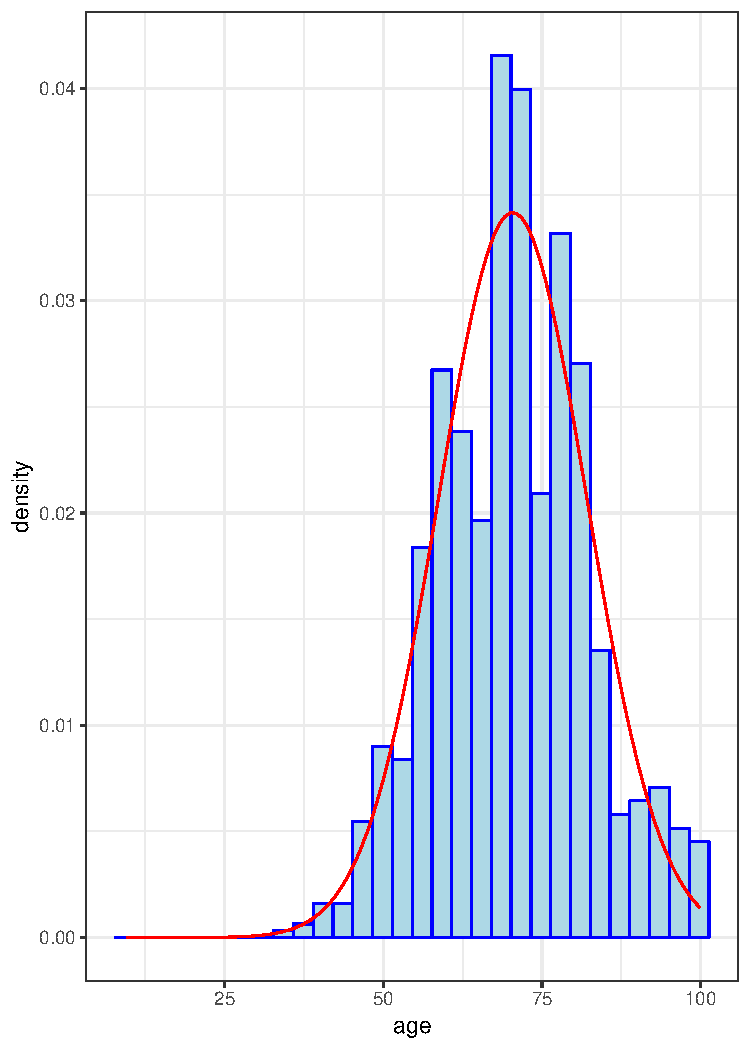
\includegraphics[scale = .8]{../../data-raw/figs/age-density.pdf}
\caption{Age distribution of patients with cancer of the lung and bronchus}\label{fig:age-distribution}
\end{figure}


\section{Systematic Literature Review}\label{app:slr}

\subsection{Treatment effects for transition rates}
Evidence to estimate treatment effects regarding efficacy and safety were obtained from RCTs identified with a systematic literature review. The scope of the review in terms of population, interventions, comparators, outcomes, and study design (PICOS) are outlined in \autoref{tbl:picos-tx-effects-1L}, \autoref{tbl:picos-tx-effects-2L}, and \autoref{tbl:picos-tx-effects-2LP}. 

\begin{table}[!ht]
\begin{center}
\begin{threeparttable}
\caption{PICOS criteria for review of treatment effects (metastatic 1L population)} \label{tbl:picos-tx-effects-1L}
\begin{tabular}{p{0.3\linewidth}p{0.7\linewidth}}
\hline
\multicolumn{1}{l}{PICOS} &  \multicolumn{1}{l}{Criteria}\\
\hline
Population & Adult patients with metastatic non-squamous NSCLC who are EGFR positive and without prior treatment for their disease.\\
&\\
Interventions & The following drugs as monotherapy or in combination with other drugs 
\begin{itemize}
\item erlotinib
\item afatinib
\item gefitinib
\item osimertinib
\item dacomitinib
\end{itemize} \\
Comparators & 
\begin{itemize}
\item placebo
\item best supportive care (BSC), defined as whichever therapy was judged to be appropriate by the treating physician.
\item any intervention of interest
\item any treatment that facilitates an indirect comparison
\end{itemize} \\
Outcomes & 
\begin{itemize}
\item OS
\item PFS
\item TTP
\end{itemize} \\
Study design & RCTs \\
&\\
Other & English language\\
\hline
\end{tabular}
\scriptsize Note: Trials where the overall study population is an all-comer population, but subgroup results are reported for the target population of interest are included. A trial or subgroup where the study population is a mixture of non-squamous and squamous patients is included if over 90\% is non-squamous. 
\end{threeparttable}
\end{center}
\end{table}


\begin{table}[!ht]
\begin{center}
\begin{threeparttable}
\caption{PICOS criteria for review of treatment effects (metastatic 2L population)} \label{tbl:picos-tx-effects-2L}
\begin{tabular}{p{0.3\linewidth}p{0.7\linewidth}}
\hline
\multicolumn{1}{l}{PICOS} &  \multicolumn{1}{l}{Criteria}\\
\hline
Population & Adult patients with metastatic non-squamous NSCLC who are EGFR+ positive and
who have experienced progression after one line of prior treatment.\\
&\\
Interventions & The following drugs as monotherapy or in combination with other drugs 
\begin{itemize}
\item erlotinib
\item afatinib
\item gefitinib
\item osimertinib
\item dacomitinib
\item nivolumab
\item pembrolizumab
\item atezolizumab
\item bevacizumab
\item platinum-based doublet therapy
\end{itemize} \\
Comparators & 
\begin{itemize}
\item placebo
\item best supportive care (BSC), defined as whichever therapy was judged to be appropriate by the treating physician.
\item any intervention of interest
\item any treatment that facilitates an indirect comparison
\end{itemize} \\
Outcomes & 
\begin{itemize}
\item OS
\item PFS
\item TTP
\end{itemize} \\
Study design & RCTs \\
&\\
Other & English language\\
\hline
\end{tabular}
\scriptsize Note: Trials where the overall study population is an all-comer population, but subgroup results are reported for the target population of interest are included. A trial or subgroup where the study population is a mixture of non-squamous and squamous patients is included if over 90\% is non-squamous.  
\end{threeparttable}
\end{center}
\end{table}

\begin{table}[!ht]
\begin{center}
\begin{threeparttable}
\caption{PICOS criteria for review of treatment effects (metastatic 2L+ population)} \label{tbl:picos-tx-effects-2LP}
\begin{tabular}{p{0.3\linewidth}p{0.7\linewidth}}
\hline
\multicolumn{1}{l}{PICOS} &  \multicolumn{1}{l}{Criteria}\\
\hline
Population & Adult patients with metastatic non-squamous NSCLC who are EGFR+ positive and
who have experienced progression after two or more prior prior treatments.\\
&\\
Interventions & The following drugs as monotherapy or in combination with other drugs 
\begin{itemize}
\item nivolumab
\item pembrolizumab
\item atezolizumab
\item bevacizumab
\item platinum-based doublet therapy
\end{itemize} \\
Comparators & 
\begin{itemize}
\item placebo
\item best supportive care (BSC), defined as whichever therapy was judged to be appropriate by the treating physician.
\item any intervention of interest
\item any treatment that facilitates an indirect comparison
\end{itemize} \\
Outcomes & 
\begin{itemize}
\item OS
\item PFS
\item TTP
\end{itemize} \\
Study design & RCTs \\
&\\
Other & English language\\
\hline
\end{tabular}
\scriptsize Note: Trials where the overall study population is an all-comer population, but subgroup results are reported for the target population of interest are included. A trial or subgroup where the study population is a mixture of non-squamous and squamous patients is included if over 90\% is non-squamous.  
\end{threeparttable}
\end{center}
\end{table}






\subsection{Utilities}
In order to identify utility values for the different (PFS and OS related) health states of the model, as well as disutility estimates associated with adverse events, a systematic search of the literature was performed to identify published (systematic) review studies. Available review studies were used to select the primary studies with estimates relevant for the model. In anticipation that there may not have been studies reporting utility estimates that could directly be used in the model, we also searched for published mapping algorithms that would allow a non-preference-based measure (generic or disease-specific measure) to be mapped onto a generic preference-based measure of interest, as well as mapping algorithms between different generic preference-based health state utility values. Details regarding eligibility criteria defining the scope of the literature review are outlined in \autoref{tbl:picos-utilities}. 


\begin{table}[!ht]
\begin{center}
\begin{threeparttable}
\caption{PICOS criteria for review of utility estimates} \label{tbl:picos-utilities}
\begin{tabular}{p{0.3\linewidth}p{0.7\linewidth}}
\hline
\multicolumn{1}{l}{PICOS} &  \multicolumn{1}{l}{Criteria}\\
\hline
Population & Adult patients with metastatic non-squamous NSCLC\\
&\\
Interventions & No restriction on inclusion of studies based on interventions or comparators\\
Outcomes & 
\begin{itemize}
\item Utility measures (e.g. EQ-5D, HUI-2, HUI-3, SF-6D) as a function of PFS, OS, TTP or adverse events
\item Mapping algorithms from a non-preference-based measure (generic or disease-specific measure) to a generic preference-based
\item Mapping algorithms between different generic preference-based health state utility values
\end{itemize} \\
Study design & 
\begin{itemize}
\item Reviews
\item Alternatively, primary studies
\end{itemize} \\
&\\
Other & 
English language\\
\hline
\end{tabular}
\end{threeparttable}
\end{center}
\end{table}




\subsection{Resource use, productivity, and cost}
Relevant evidence regarding resource use, productivity and cost estimates was identified by means of a review of published cost-of-illness studies, cost-effectiveness studies, and budget impact studies in NSCLC relevant for the US setting. Criteria defining studies considered relevant are outlined in \autoref{tbl:picos-cost}. The most recent studies reporting relevant estimates among EGFR+NSCLC patients treated with TKIs were used in the economic model.

\begin{table}[!ht]
\begin{center}
\begin{threeparttable}
\caption{PICOS criteria for studies providing information on resource use, productivity, and cost estimates} \label{tbl:picos-cost}
\begin{tabular}{p{0.3\linewidth}p{0.7\linewidth}}
\hline
\multicolumn{1}{l}{PICOS} &  \multicolumn{1}{l}{Criteria}\\
\hline
Population & Adult patients with metastatic non-squamous NSCLC\\
&\\
Interventions & No restriction on inclusion of studies based on interventions or comparators\\
Outcomes & 
\begin{itemize}
\item Resource use
\item Cost
\item Productivity
\end{itemize} \\
Study design &  
\begin{itemize}
\item Cost-of-illness studies
\item Cost-effectiveness studies
\item Budget impact studies
\end{itemize} \\
&\\
Other & 
English language\\
\hline
\end{tabular}
\end{threeparttable}
\end{center}
\end{table}

\subsection{Study identification}
Relevant clinical studies were identified by searching the following databases using predefined search strategies: Medical Literature Analysis and Retrieval System Online (MEDLINE), Excerpta Medica database (EMBASE), and Cochrane Central Register of Controlled Trials. The study design filters recommended by the Scottish Intercollegiate Guidelines Network (SIGN) for MEDLINE and EMBASE were used to identify clinical trials. The search included terms related to the generic and brand name of the interventions of interest. Search strategies are available in the MS Excel spreadsheet available on GitHub.

For utility studies and studies providing evidence on healthcare utilization and costs, the following databases were searched: MEDLINE, EMBASE, NHS Economic Evaluation Database (NHS EED), The Health Economics Research Centre (HERC)-maintained mapping algorithm database, and The University of Sheffield's ScHARRHUD database of health utilities' evidence.

Search strategies are available in the spreadsheets available on GitHub.

\subsection{Study selection}
For the review of clinical evidence, two reviewers, working independently, reviewed all abstracts identified with each of the searches according to the selection criteria, with the exception of outcome criteria in the efficacy and safety searches, which were only applied during the screening of full-text publications. All studies identified as eligible studies during abstract screening were then screened at a full-text stage by the same two reviewers. The full-text studies identified at this stage were included for data extraction. Following reconciliation between the two investigators, a third reviewer was included to reach consensus for any remaining discrepancies. The process of study identification and selection is summarized with a Preferred Reporting Items for Systematic Reviews and Meta-Analyses (PRISMA) flow diagram. 

For the review of utility studies and studies providing evidence on healthcare utilization and costs, this process was performed by a single reviewer and findings checked by a second-reviewer. 

\subsection{Data collection}
For the clinical studies, two reviewers, working independently, extracted data on study characteristics, interventions, patient characteristics, and outcomes for the final list of included studies. Following reconciliation between the two reviewers, a third reviewer was included to reach consensus on any remaining discrepancies. For all outcomes of interest, information regarding point estimates, variability and uncertainty was obtained. For PFS and OS, hazard ratios and associated information regarding uncertainty were extracted. If results were reported as forest plots, the point estimate and 95\$ percent\ confidence interval were extracted using DigitizeIt software version 2.1.4 (Bormisoft - Informer Technologies, Inc.). Kaplan Meier curves will also be digitzed using DigitizeIt and the proportion of patients free of the event over time will be extracted and the number of patients at risk over time. Adverse events were collected, if reported. 

For utility and cost-effectiveness studies, relevant information for the model was extracted from the source publications and checked by a second-reviewer. 

Spreadsheets with extracted data are available on GitHub.

\subsection{Limitations}
Despite the strengths of the systematic literature review to identify relevant evidence, some limitations should be acknowledged. First, the scope of the review was restricted to studies published in English. Second, the evidence base is continually growing and at some point the studies used for model input parameter estimates may no longer reflect the latest data. This may especially be the case for the efficacy of osimertinib and dacomitinib. Third, there is always a risk of publication or outcome reporting bias. Finally, the information obtained from the literature and used in the model may not be an accurate reflection of a local setting.

\section{Evidence base, clinical}
\subsection{Study identification and selection} \label{app:study-selection}
The identification and selection of relevant studies used to estimate treatment effects is summarized with \autoref{fig:slr-flow}.Detailed results regarding the screening and selection process are available in the spreadsheet available on GitHub.


\begin{figure}
\centering
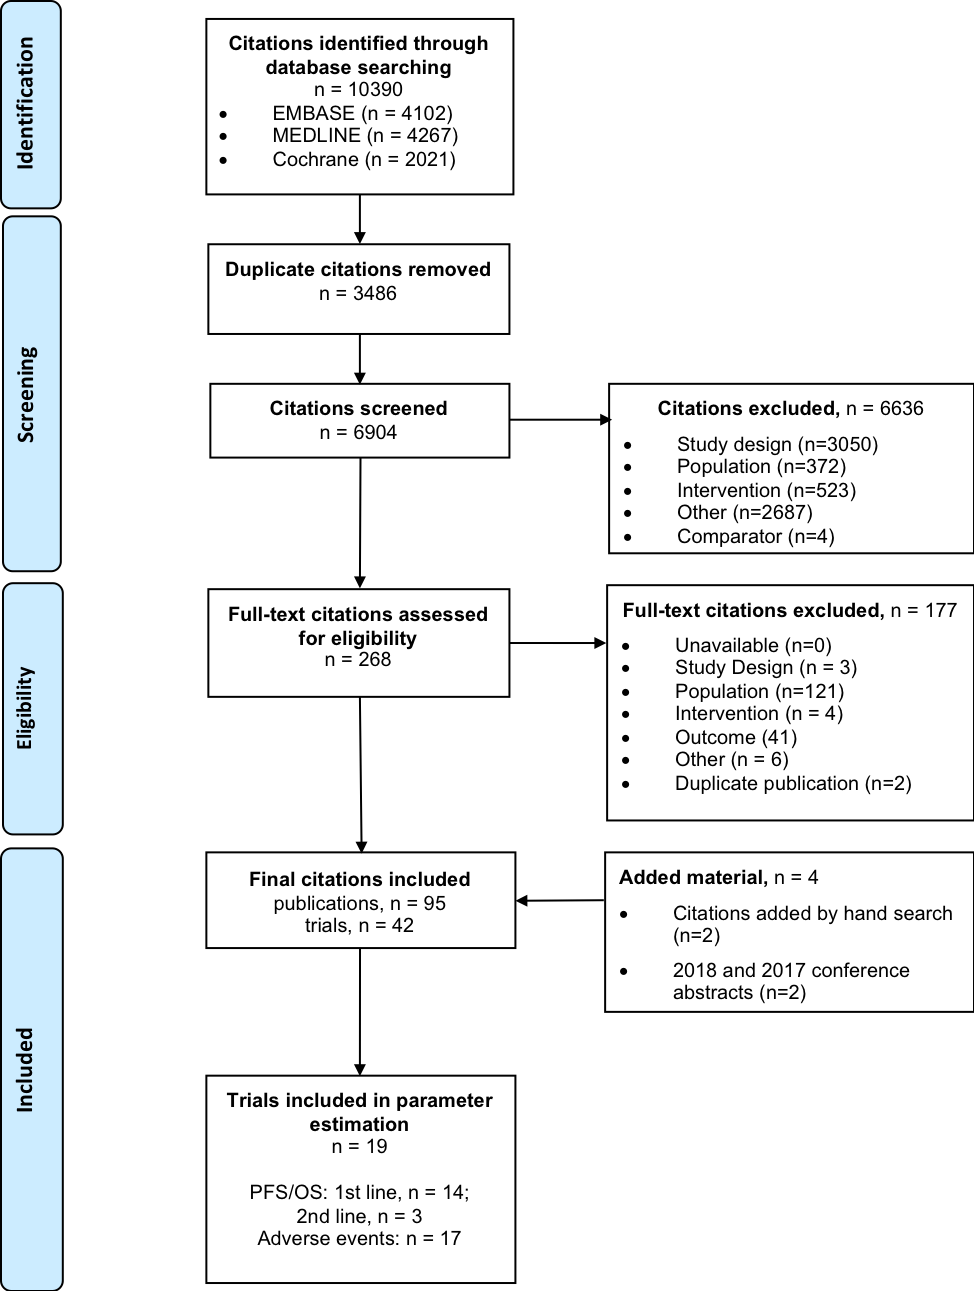
\includegraphics[max size={\textwidth}{\textheight}]{figs/flow diagram SLR.png}
\caption{Study identification and selection}\label{fig:slr-flow}
\end{figure}


\subsection{Study characteristics} \label{app:study-characteristics}
In .... information regarding study design characteristics is provided for the studies used to estimate PFS and OS. 

\subsection{Treatment characteristics} \label{app:treatment-characteristics}
In .... information regarding characteristics of the interventions evaluated in the studies used to estimate PFS and OS is provided.


\subsection{Patient characteristics} \label{app:patient-characteristics}

... provides information on the study populations of the different studies used to estimate PFS and OS. \autoref{fig:female-1l}-\autoref{fig:currentformermoker-1l} shows the distribution of key characteristics across the studies. 

\begin{figure}
\centering
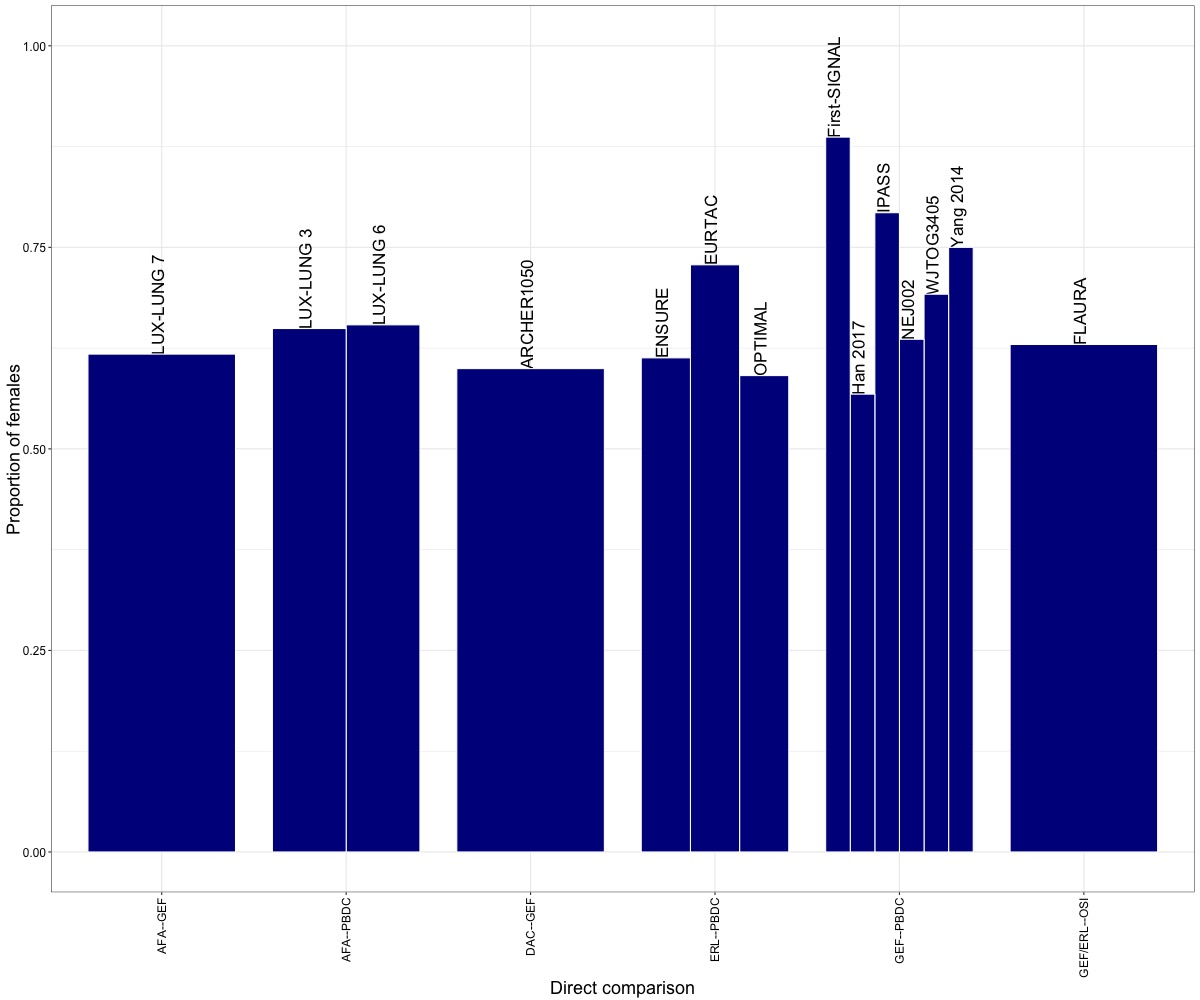
\includegraphics[max size={\textwidth}{\textheight}]{figs/dist-patchar-plots/female 1L.jpg}
\caption{Proportion of women in 1L studies}\label{fig:female-1l}
\end{figure}

\begin{figure}
\centering
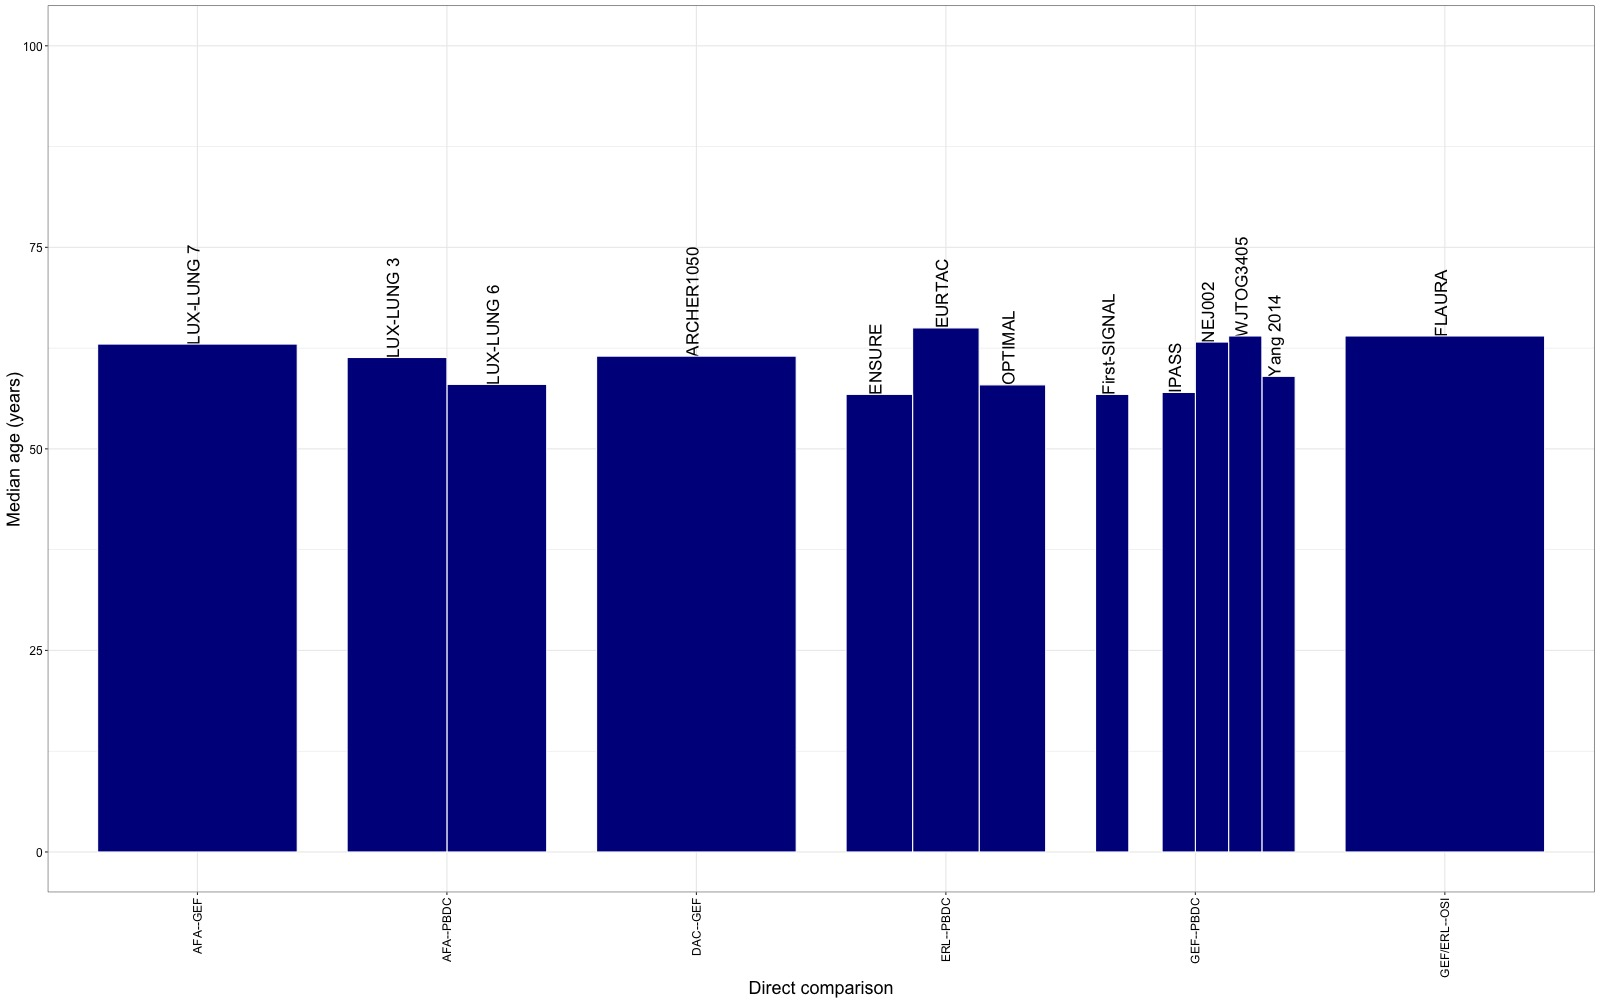
\includegraphics[max size={\textwidth}{\textheight}]{figs/dist-patchar-plots/age 1L.jpg}
\caption{Median age in 1L studies}\label{fig:age-1l}
\end{figure}

\begin{figure}
\centering
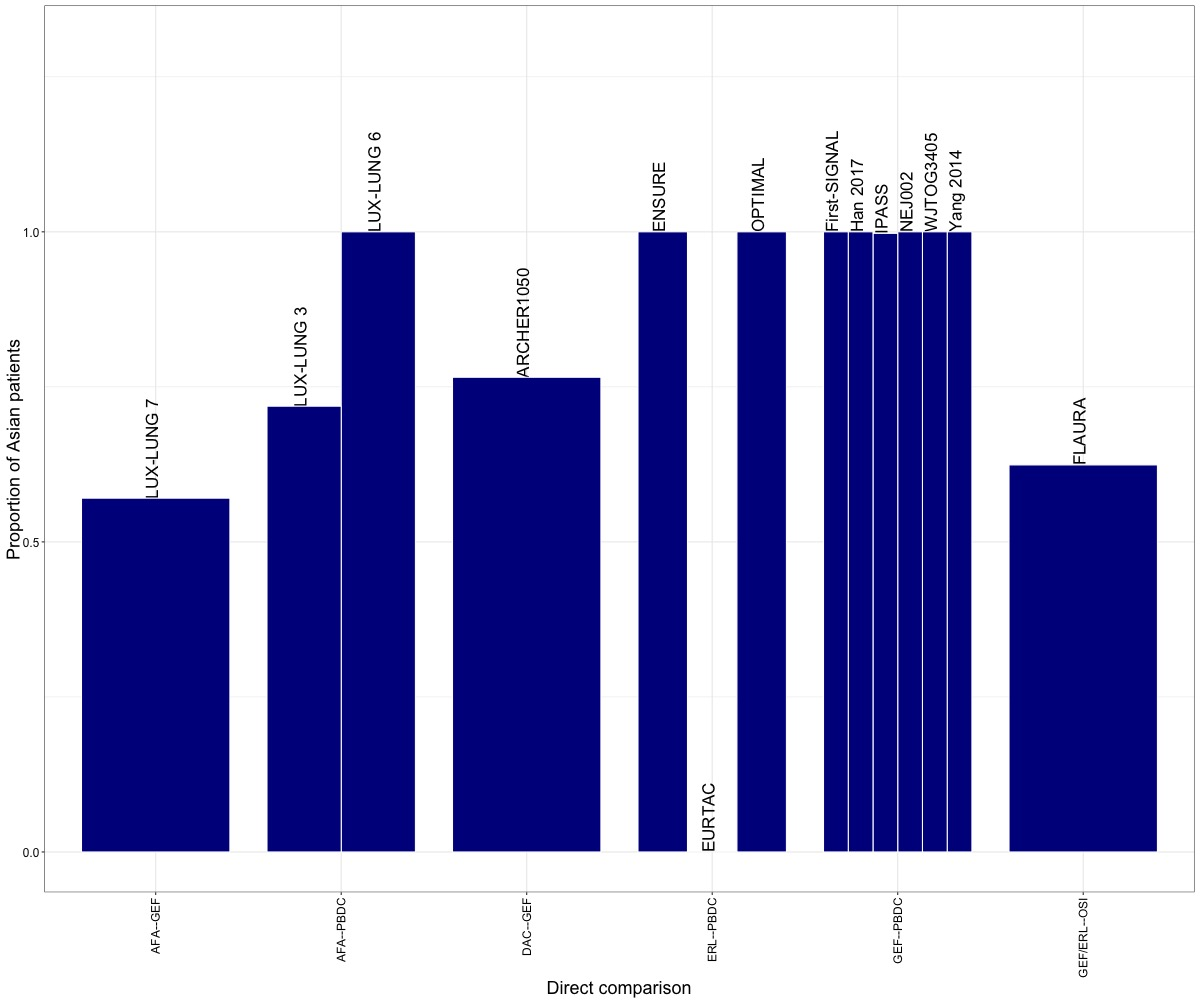
\includegraphics[max size={\textwidth}{\textheight}]{figs/dist-patchar-plots/prop asian 1L.jpg}
\caption{Proportion of Asian patients in 1L studies}\label{fig:asian-1l}
\end{figure}

\begin{figure}
\centering
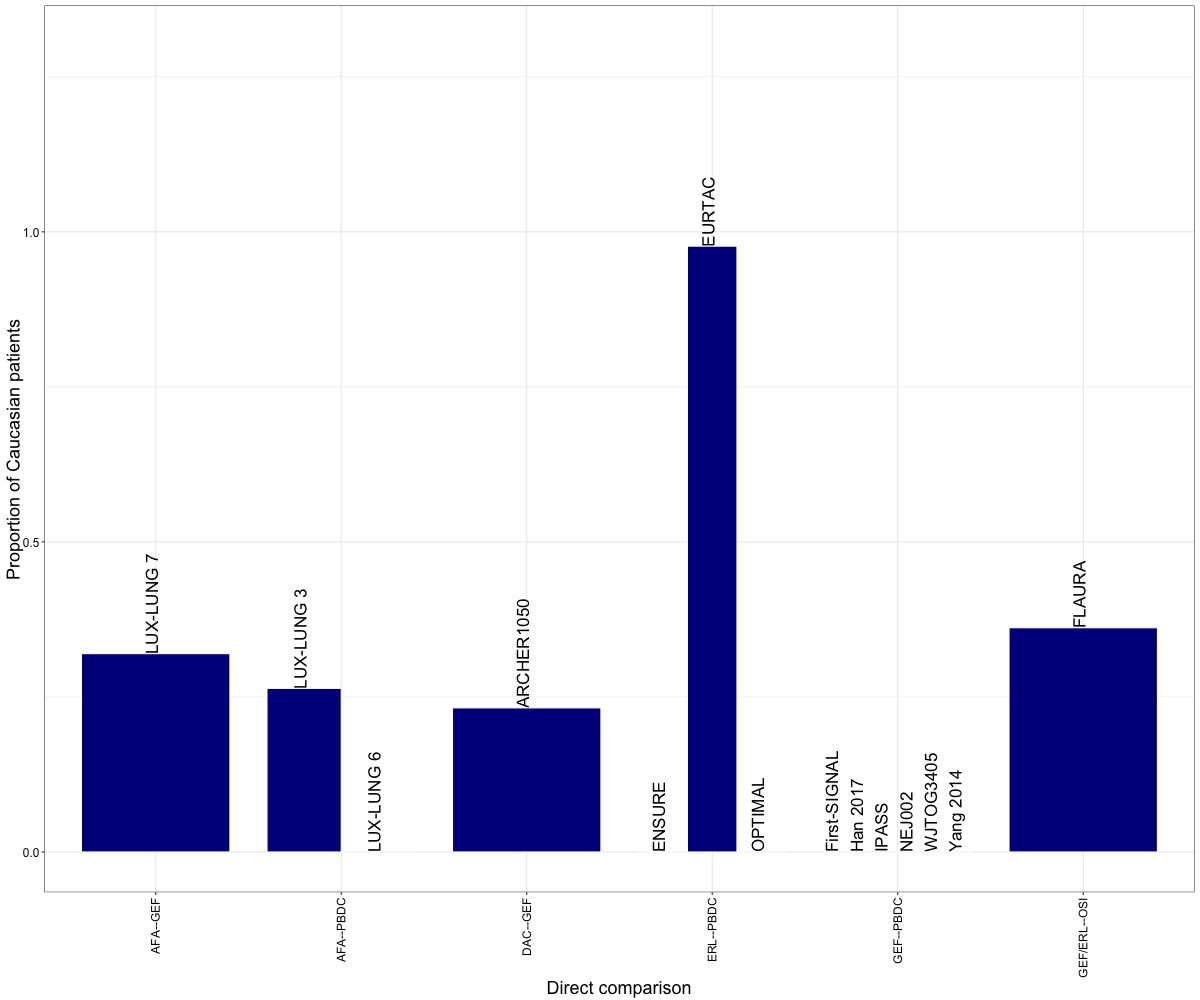
\includegraphics[max size={\textwidth}{\textheight}]{figs/dist-patchar-plots/prop white 1L.jpg}
\caption{Proportion of Caucasian patients in 1L studies}\label{fig:white-1l}
\end{figure}

\begin{figure}
\centering
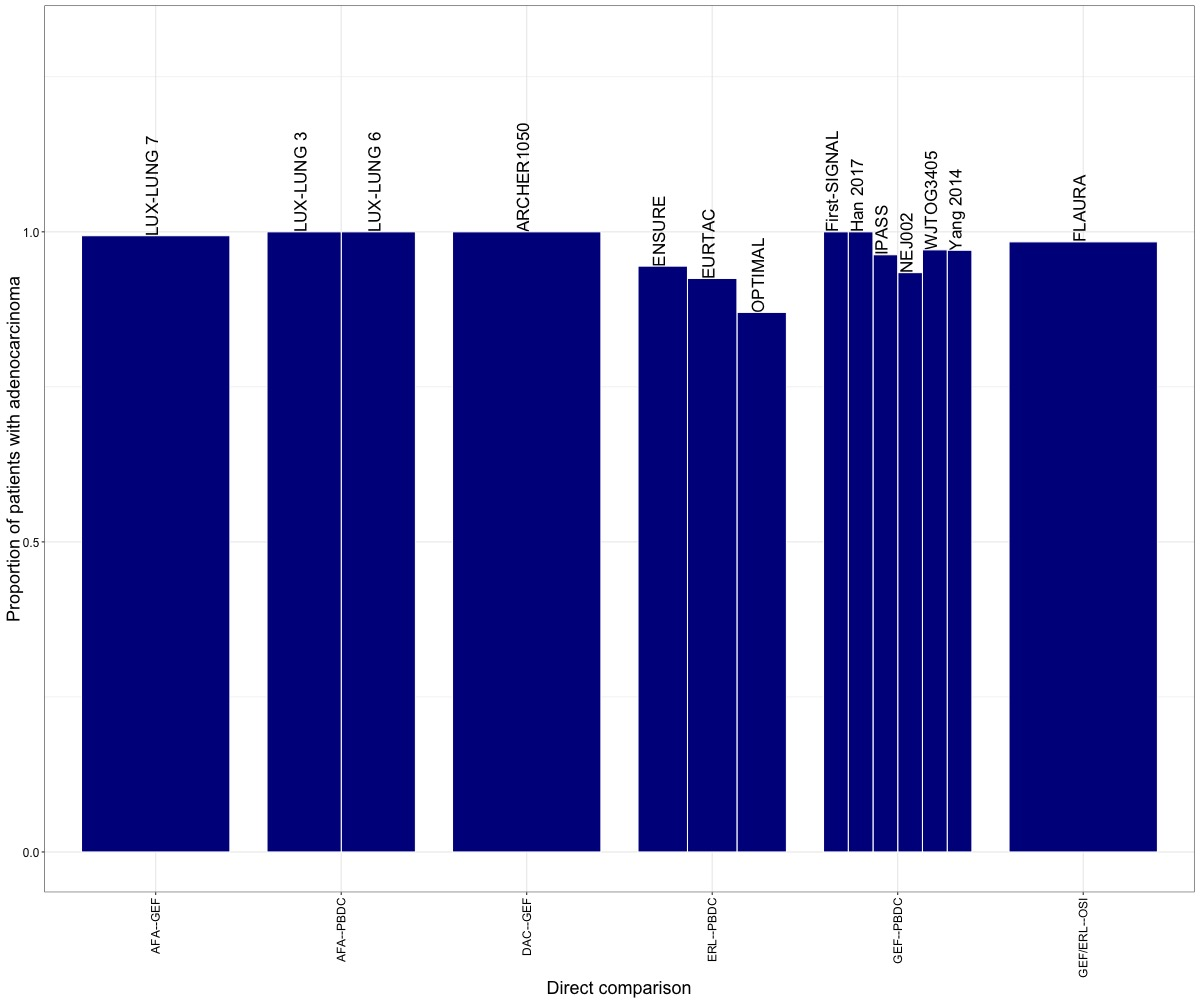
\includegraphics[max size={\textwidth}{\textheight}]{figs/dist-patchar-plots/prop adenocarcinoma 1L.jpg}
\caption{Proportion of patient with adenocarcinoma in 1L studies}\label{fig:adeno-1l}
\end{figure}

\begin{figure}
\centering
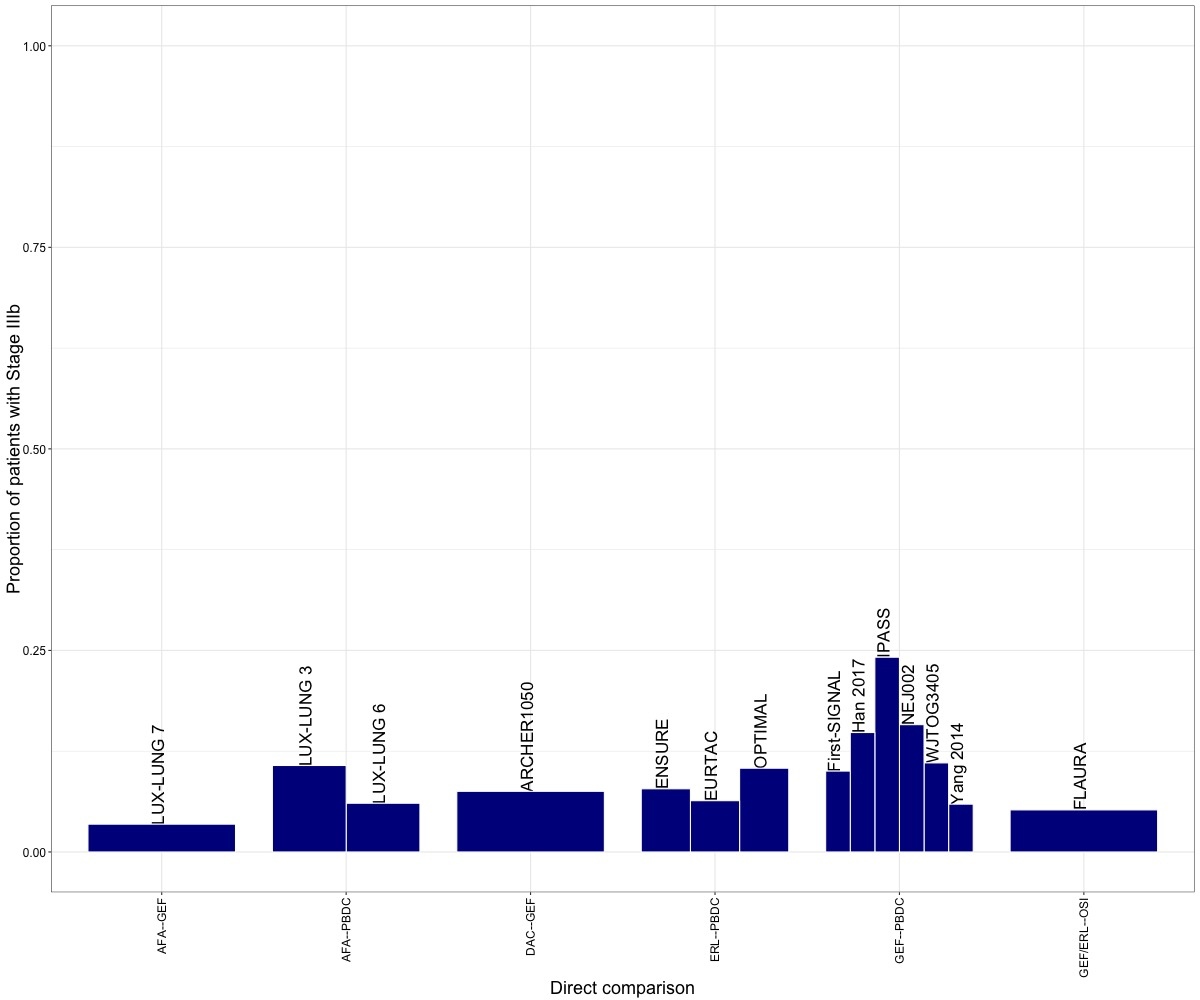
\includegraphics[max size={\textwidth}{\textheight}]{figs/dist-patchar-plots/prop stage IIIb 1L.jpg}
\caption{Proportion of patients with stage 3b disease in 1L studies}\label{fig:stageiiib-1l}
\end{figure}

\begin{figure}
\centering
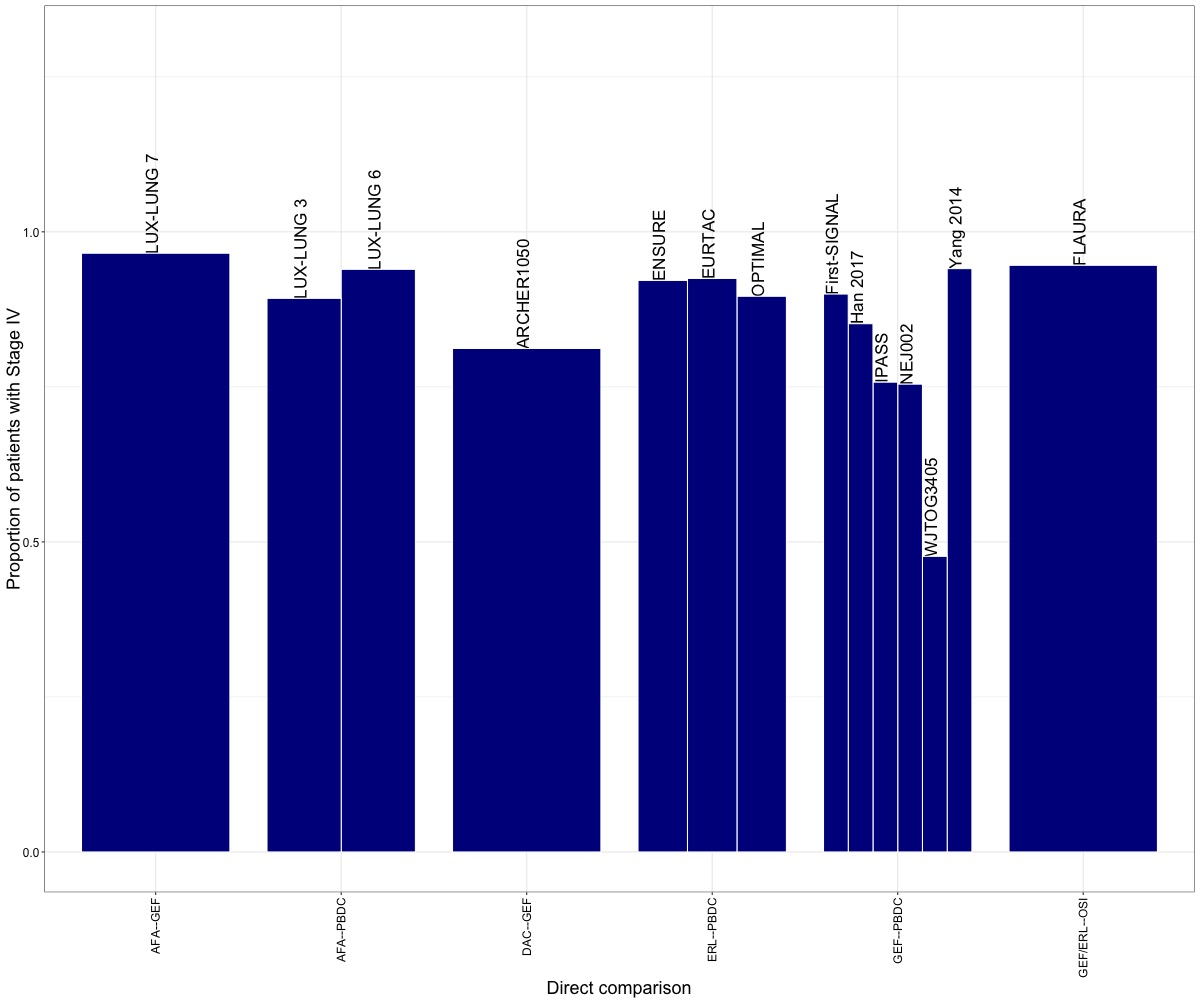
\includegraphics[max size={\textwidth}{\textheight}]{figs/dist-patchar-plots/prop stage IV 1L.jpg}
\caption{Proportion of patients with stage 4 disease in 1L studies}\label{fig:stageiv-1l}
\end{figure}

\begin{figure}
\centering
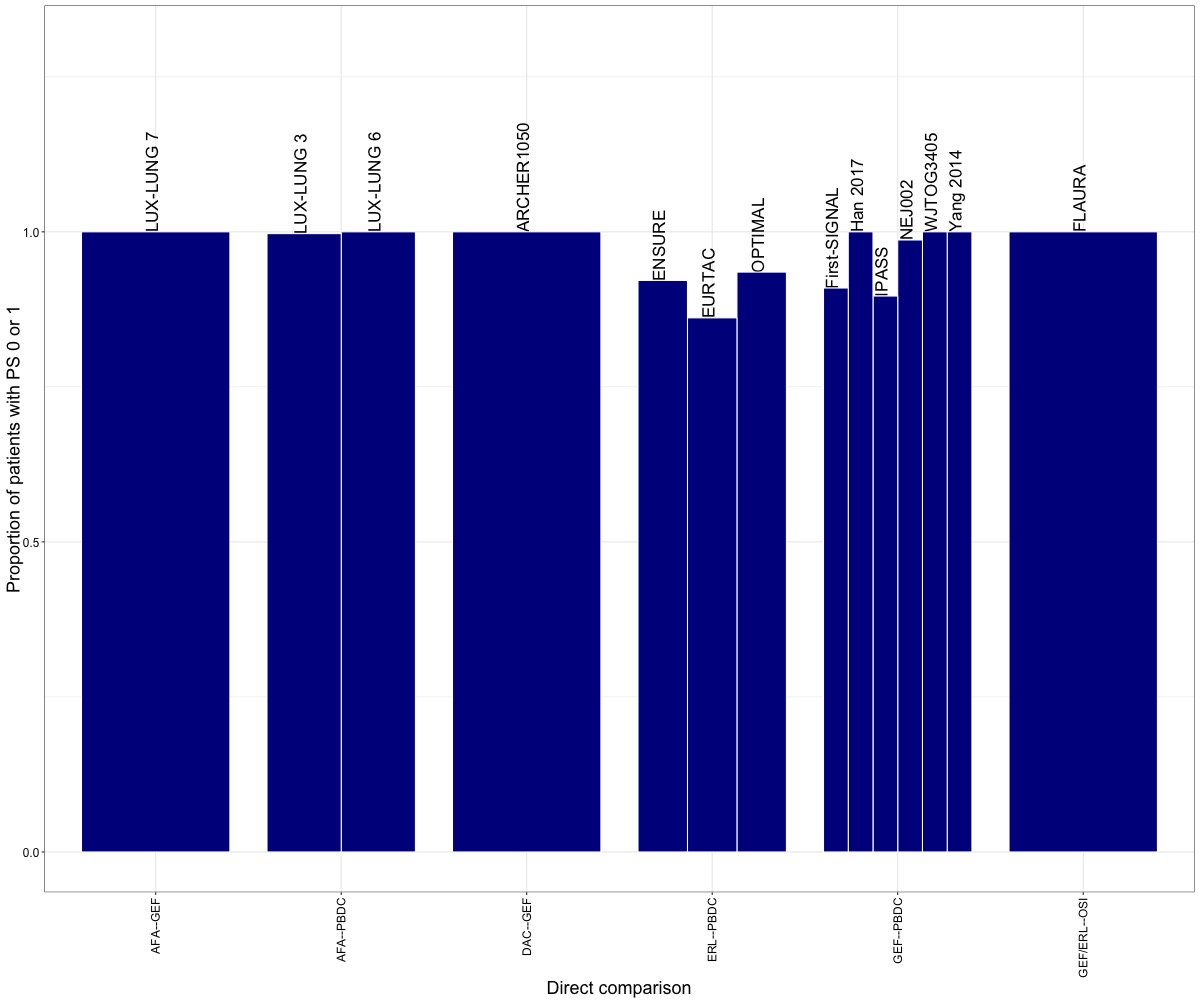
\includegraphics[max size={\textwidth}{\textheight}]{figs/dist-patchar-plots/prop PS 0 or 1 1L.jpg}
\caption{Proportion of patients with performance status 0 or 1 in 1L studies}\label{fig:ps01-1l}
\end{figure}

\begin{figure}
\centering
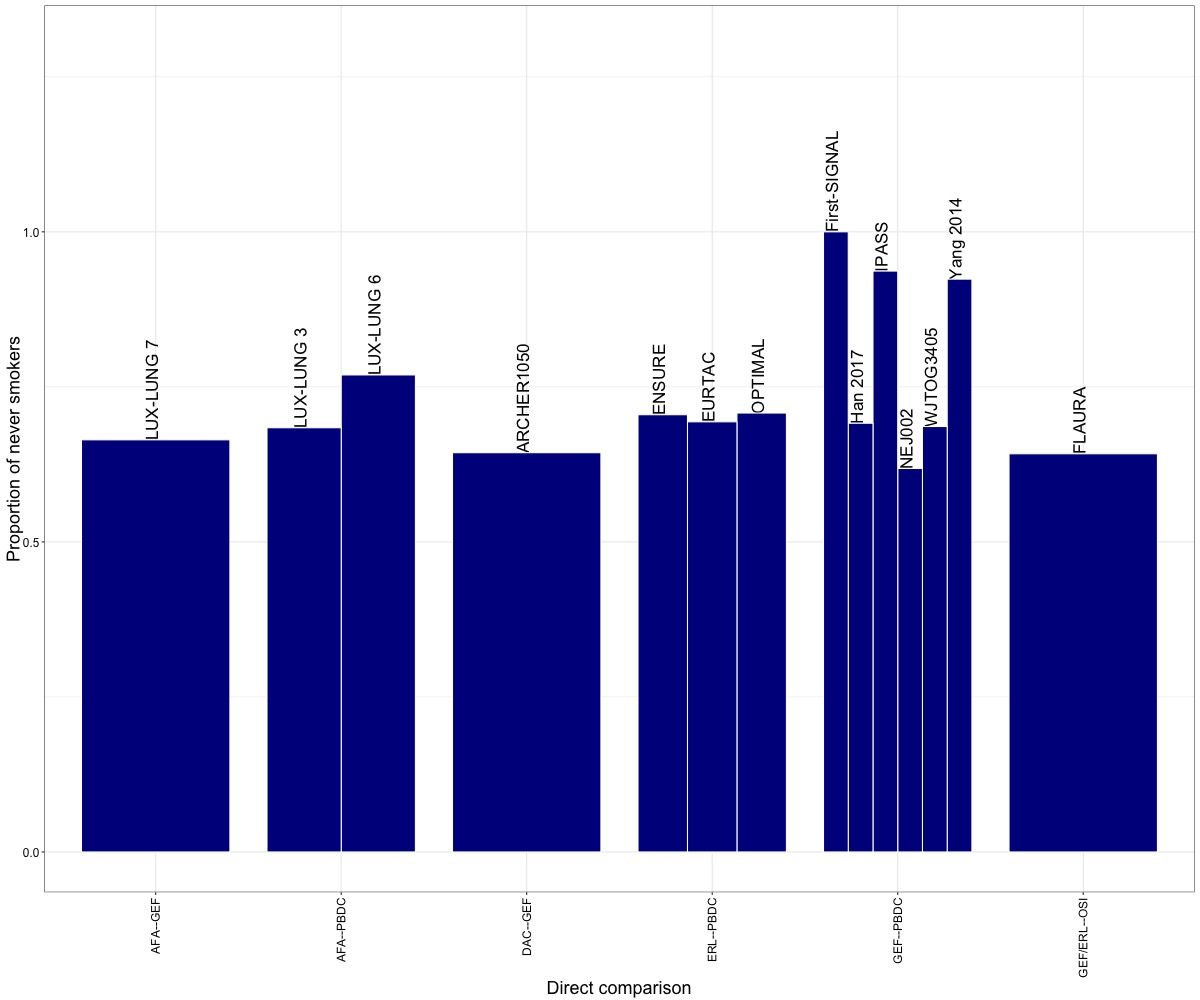
\includegraphics[max size={\textwidth}{\textheight}]{figs/dist-patchar-plots/never smoker 1L.jpg}
\caption{Proportion of never smokers in 1L studies}\label{fig:neversmoker-1l}
\end{figure}

\begin{figure}
\centering
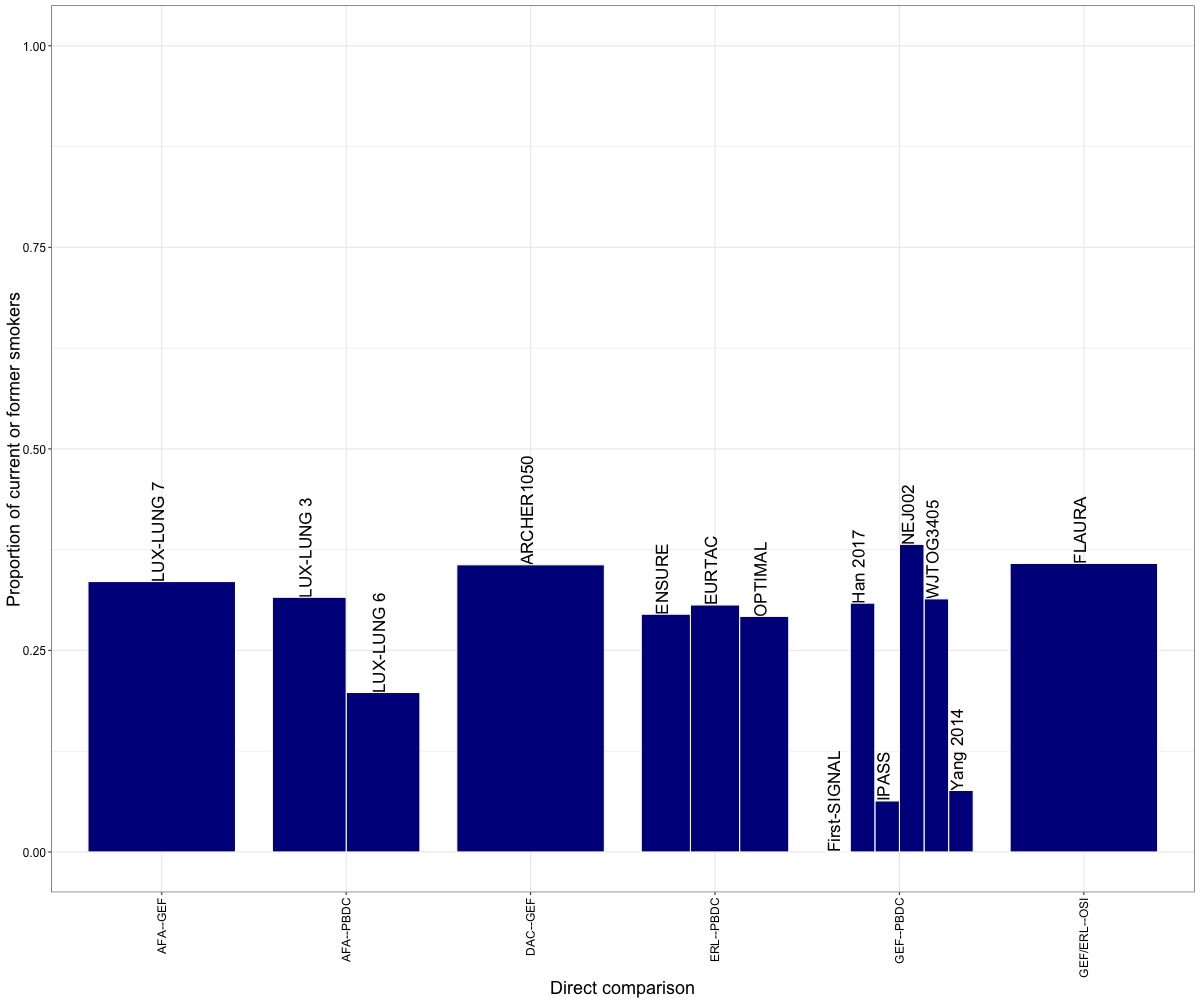
\includegraphics[max size={\textwidth}{\textheight}]{figs/dist-patchar-plots/current former smoker 1L.jpg}
\caption{Proportion of current or former smokers in 1L studies}\label{fig:currentformermoker-1l}
\end{figure}

\begin{sidewaystable}[h]
\begin{center}
\begin{threeparttable}
\caption{Patient characteristics in 1L studies, demographics and health behavior} \label{tbl:patchar-1-1L}
\tiny
\begin{tabularx}{\textwidth}{@{\extracolsep{\fill}}llp{0.20\linewidth}rrrrrrrrrr}
\hline
\multicolumn{3}{c}{} & \multicolumn{3}{c}{Age} & \multicolumn{1}{c}{} & \multicolumn{2}{c}{Race/ethnicity (\%)} & \multicolumn{4}{c}{Smoking status (\%)}\\
\cmidrule(r){4-6} \cmidrule(r){8-9} \cmidrule(r){10-13}
\multicolumn{11}{c}{} & \multicolumn{1}{r}{Current or} & \multicolumn{1}{r}{}\\
\multicolumn{1}{l}{Trial} & \multicolumn{1}{l}{Population} & \multicolumn{1}{l}{Treatment} &
\multicolumn{1}{r}{Median} & \multicolumn{1}{r}{Min} & \multicolumn{1}{r}{Max} & \multicolumn{1}{r}{Female} & \multicolumn{1}{r}{Caucasian} & \multicolumn{1}{r}{Asian} & \multicolumn{1}{r}{Former} & \multicolumn{1}{r}{Current} & \multicolumn{1}{r}{former} & \multicolumn{1}{r}{Never}\\
\hline
\ExpandableInput{tables/patchar-1-1L.txt}
\hline
\end{tabularx}
\end{threeparttable}
\end{center}
\end{sidewaystable}

\begin{sidewaystable}[h]
\begin{center}
\begin{threeparttable}
\caption{Patient characteristics in 2L studies, demographics and health behavior} \label{tbl:patchar-1-2L}
\tiny
\begin{tabularx}{\textwidth}{@{\extracolsep{\fill}}llp{0.20\linewidth}rrrrrrrrrr}
\hline
\multicolumn{3}{c}{} & \multicolumn{3}{c}{Age} & \multicolumn{1}{c}{} & \multicolumn{2}{c}{Race/ethnicity (\%)} & \multicolumn{4}{c}{Smoking status (\%)}\\
\cmidrule(r){4-6} \cmidrule(r){8-9} \cmidrule(r){10-13}
\multicolumn{11}{c}{} & \multicolumn{1}{r}{Current or} & \multicolumn{1}{r}{}\\
\multicolumn{1}{l}{Trial} & \multicolumn{1}{l}{Population} & \multicolumn{1}{l}{Treatment} &
\multicolumn{1}{r}{Median} & \multicolumn{1}{r}{Min} & \multicolumn{1}{r}{Max} & \multicolumn{1}{r}{Female} & \multicolumn{1}{r}{Caucasian} & \multicolumn{1}{r}{Asian} & \multicolumn{1}{r}{Former} & \multicolumn{1}{r}{Current} & \multicolumn{1}{r}{former} & \multicolumn{1}{r}{Never}\\
\hline
\ExpandableInput{tables/patchar-1-2L.txt}
\hline
\end{tabularx}
\end{threeparttable}
\end{center}
\end{sidewaystable}


\subsection{Kaplan-Meier curves} \label{app:km-curves}
\subsubsection{1L treatment}
%\iffalse

\begin{figure}
\centering
\begin{subfigure}{\textwidth}
\centering
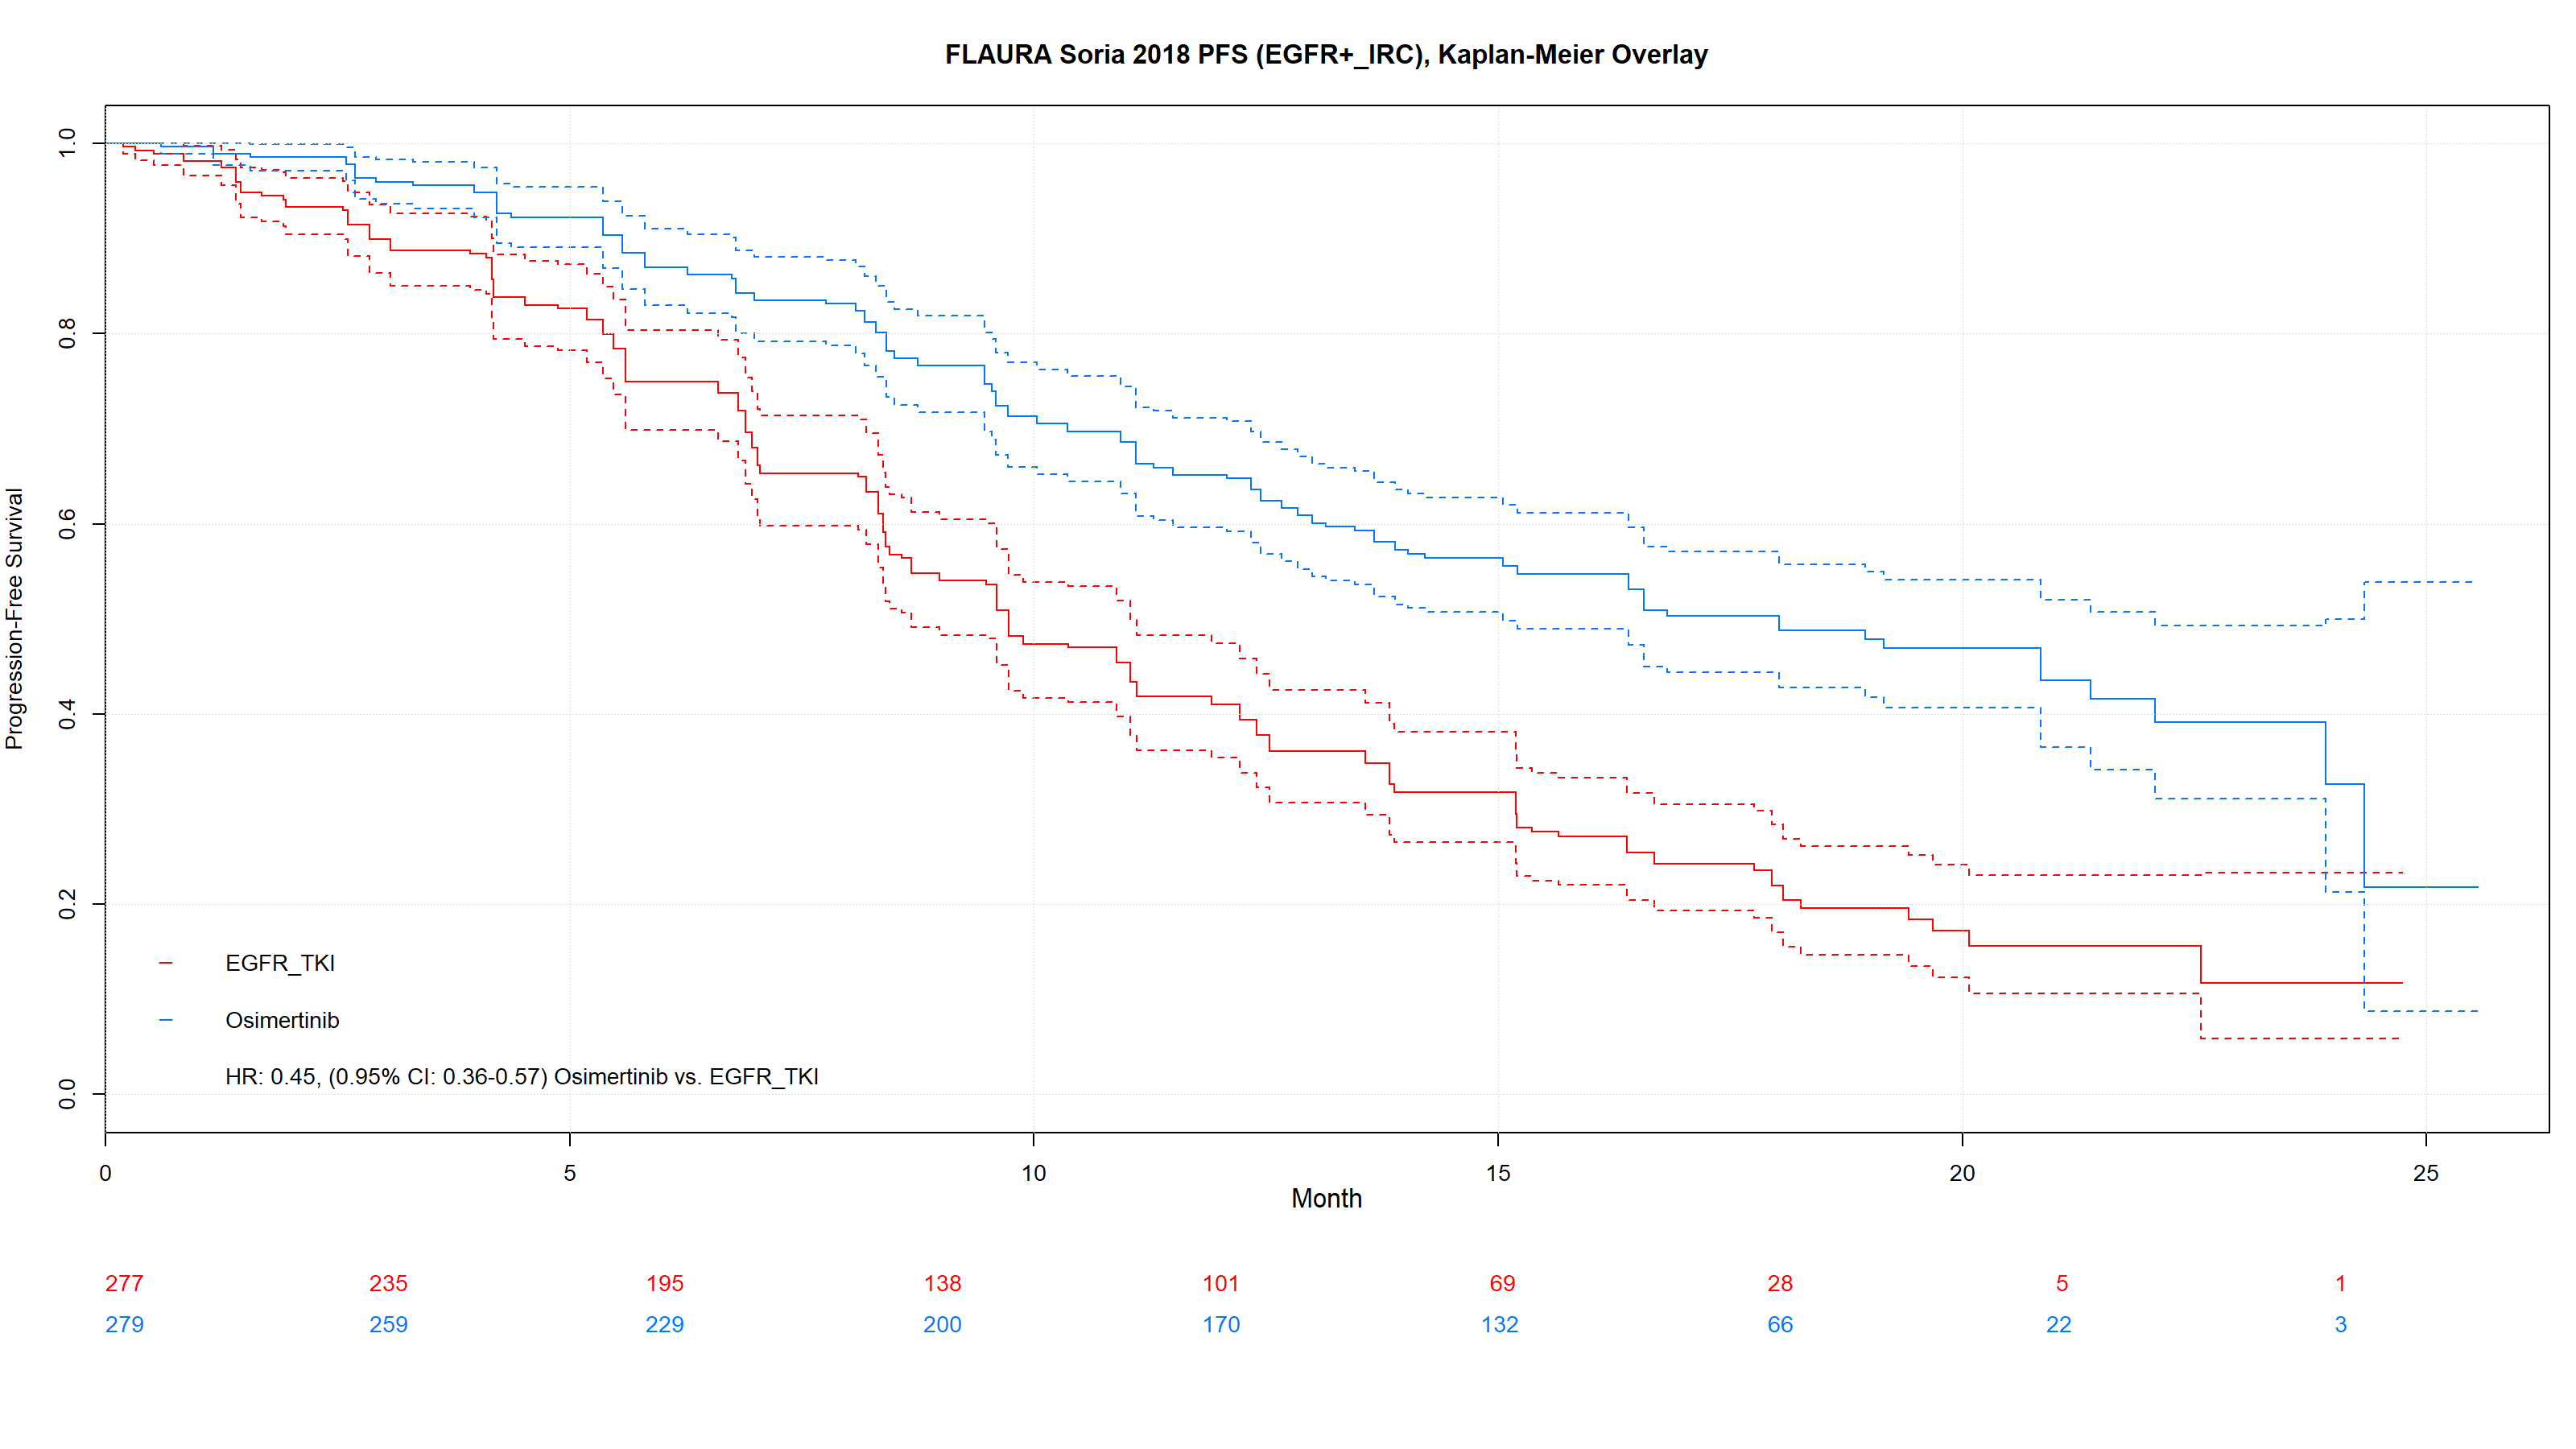
\includegraphics[max size={\textwidth}{\textheight}]{figs/km-plots/FLAURA Soria 2018 PFS (EGFR+_IRC) Kaplan Meier.png}
\end{subfigure}
\begin{subfigure}{\textwidth}
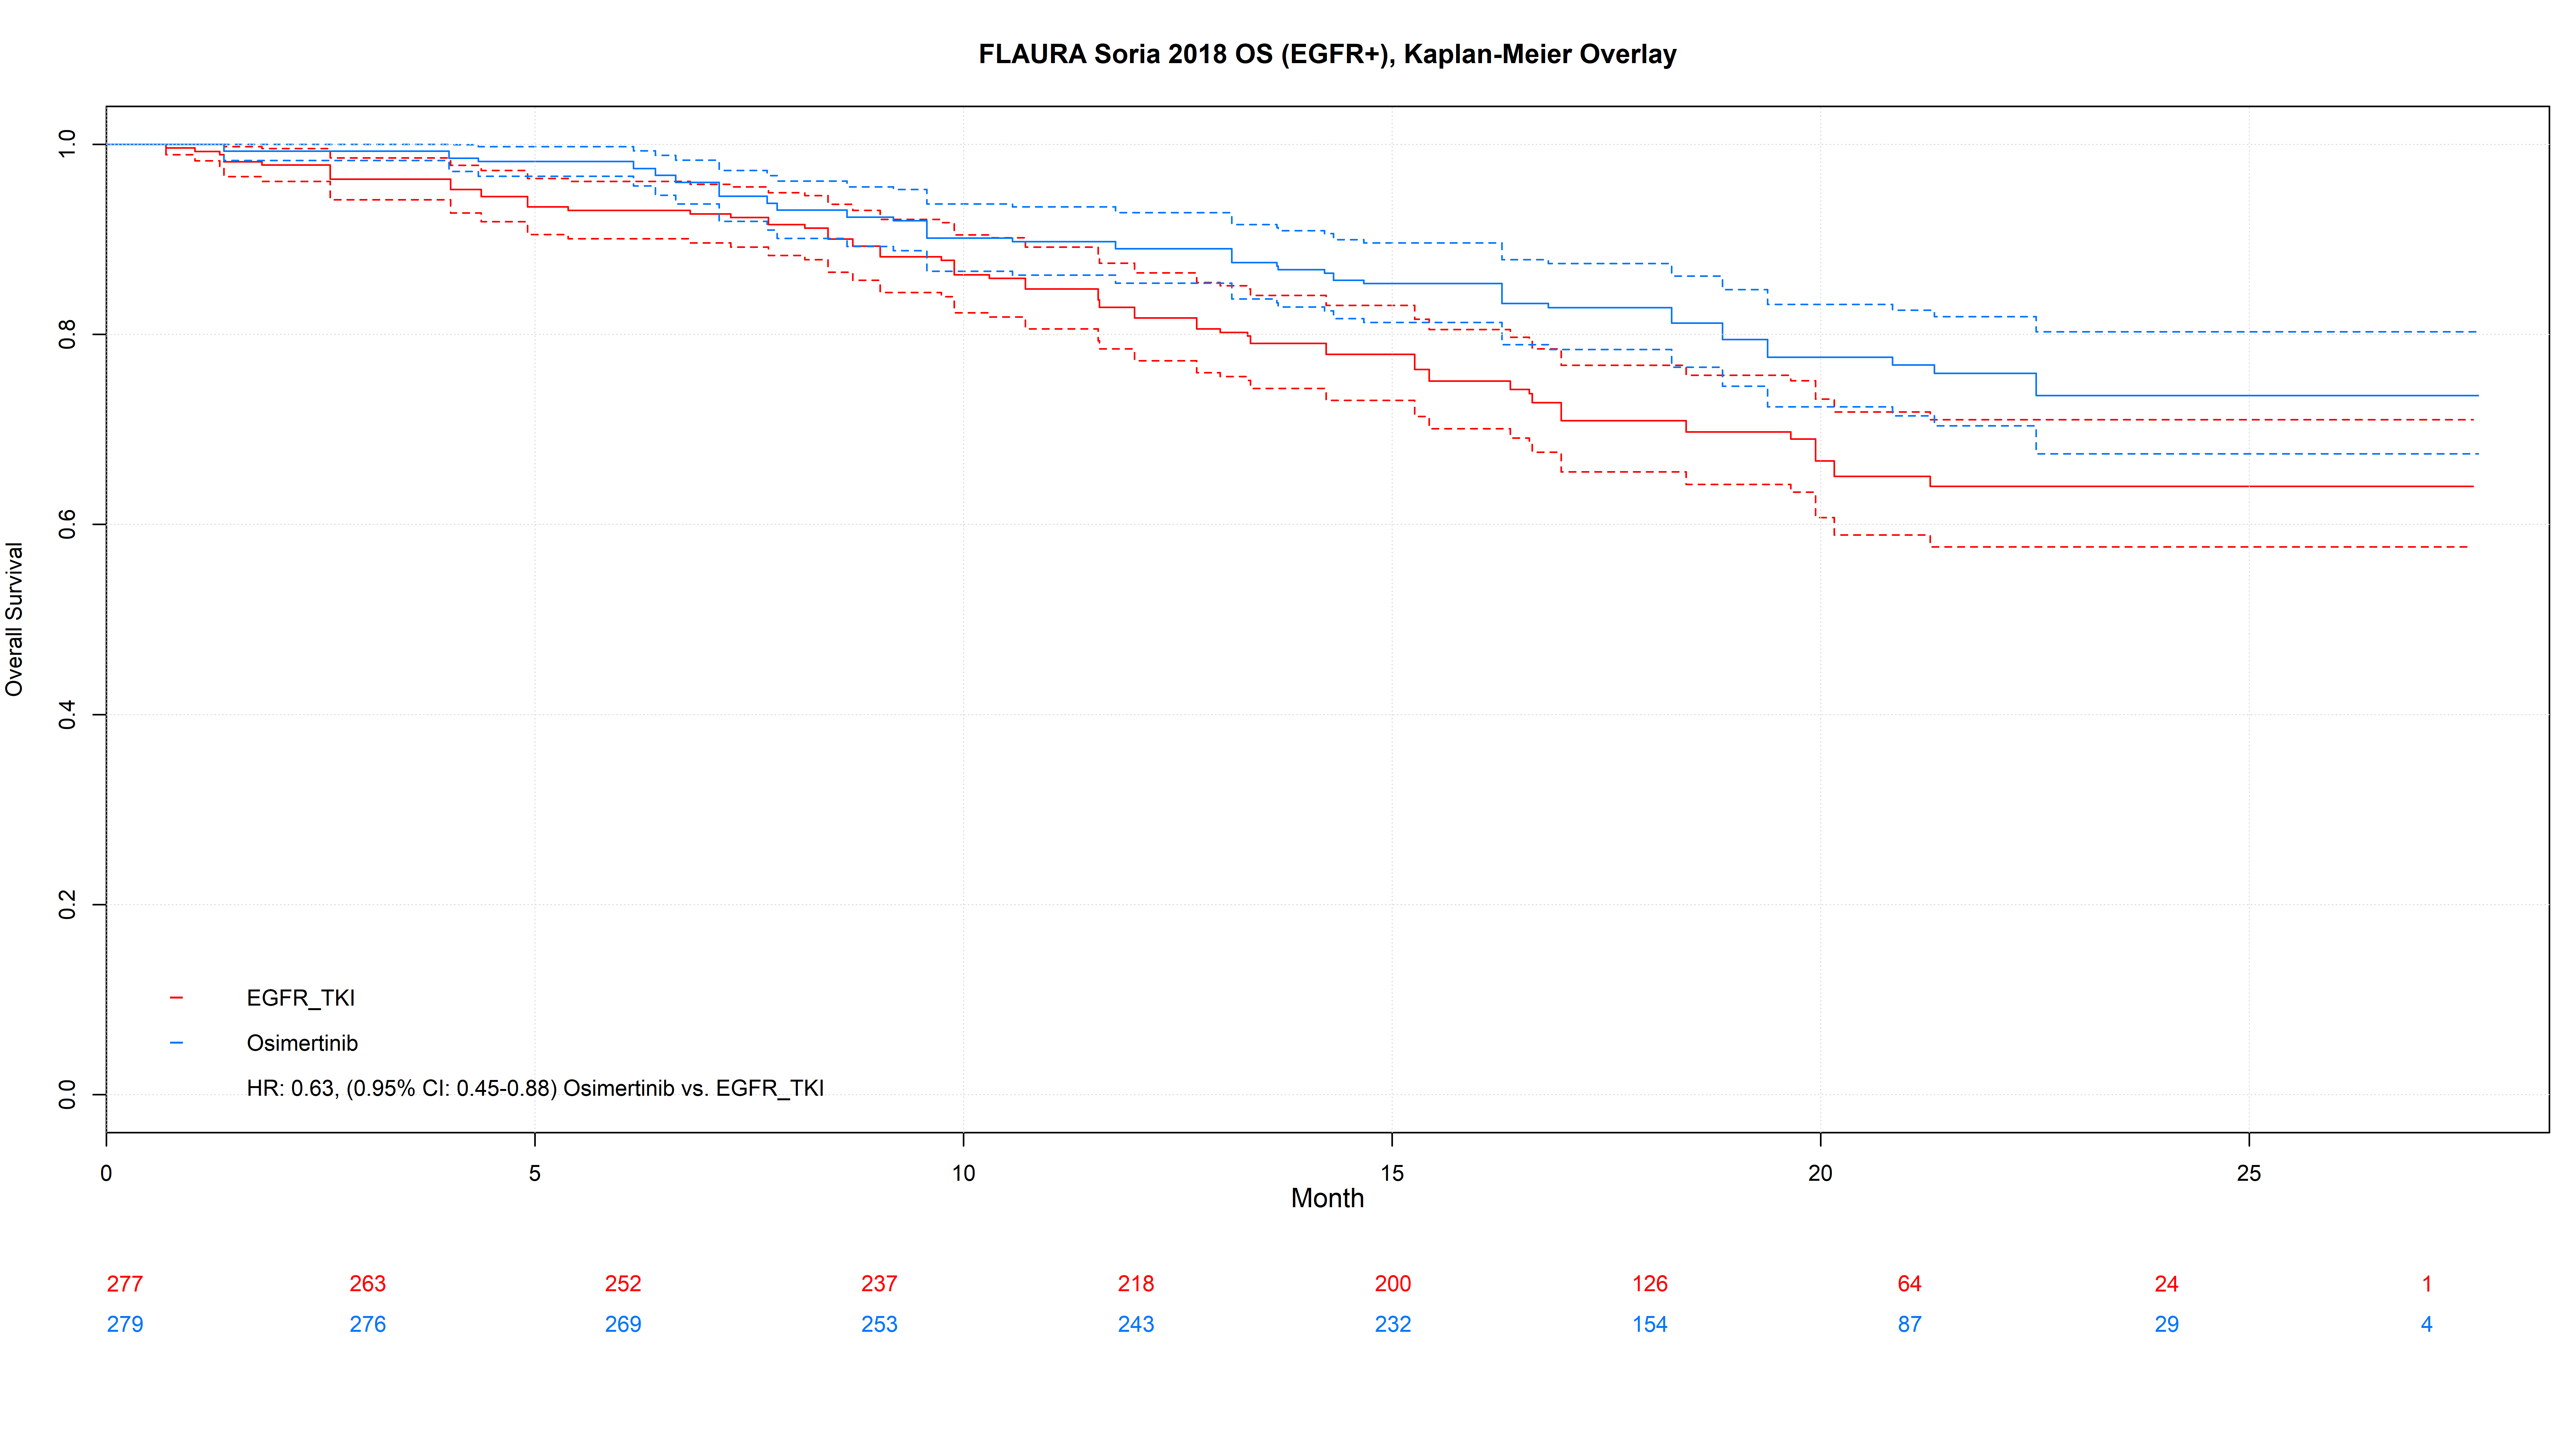
\includegraphics[max size={\textwidth}{\textheight}]{figs/km-plots/FLAURA Soria 2018 OS (EGFR+) Kaplan Meier.png}
\end{subfigure}
\centering
\caption{FLAURA, progression-free survival and overall survival}\label{fig:FLAURA}
\end{figure}


\begin{figure}
\centering
\begin{subfigure}{\textwidth}
\centering
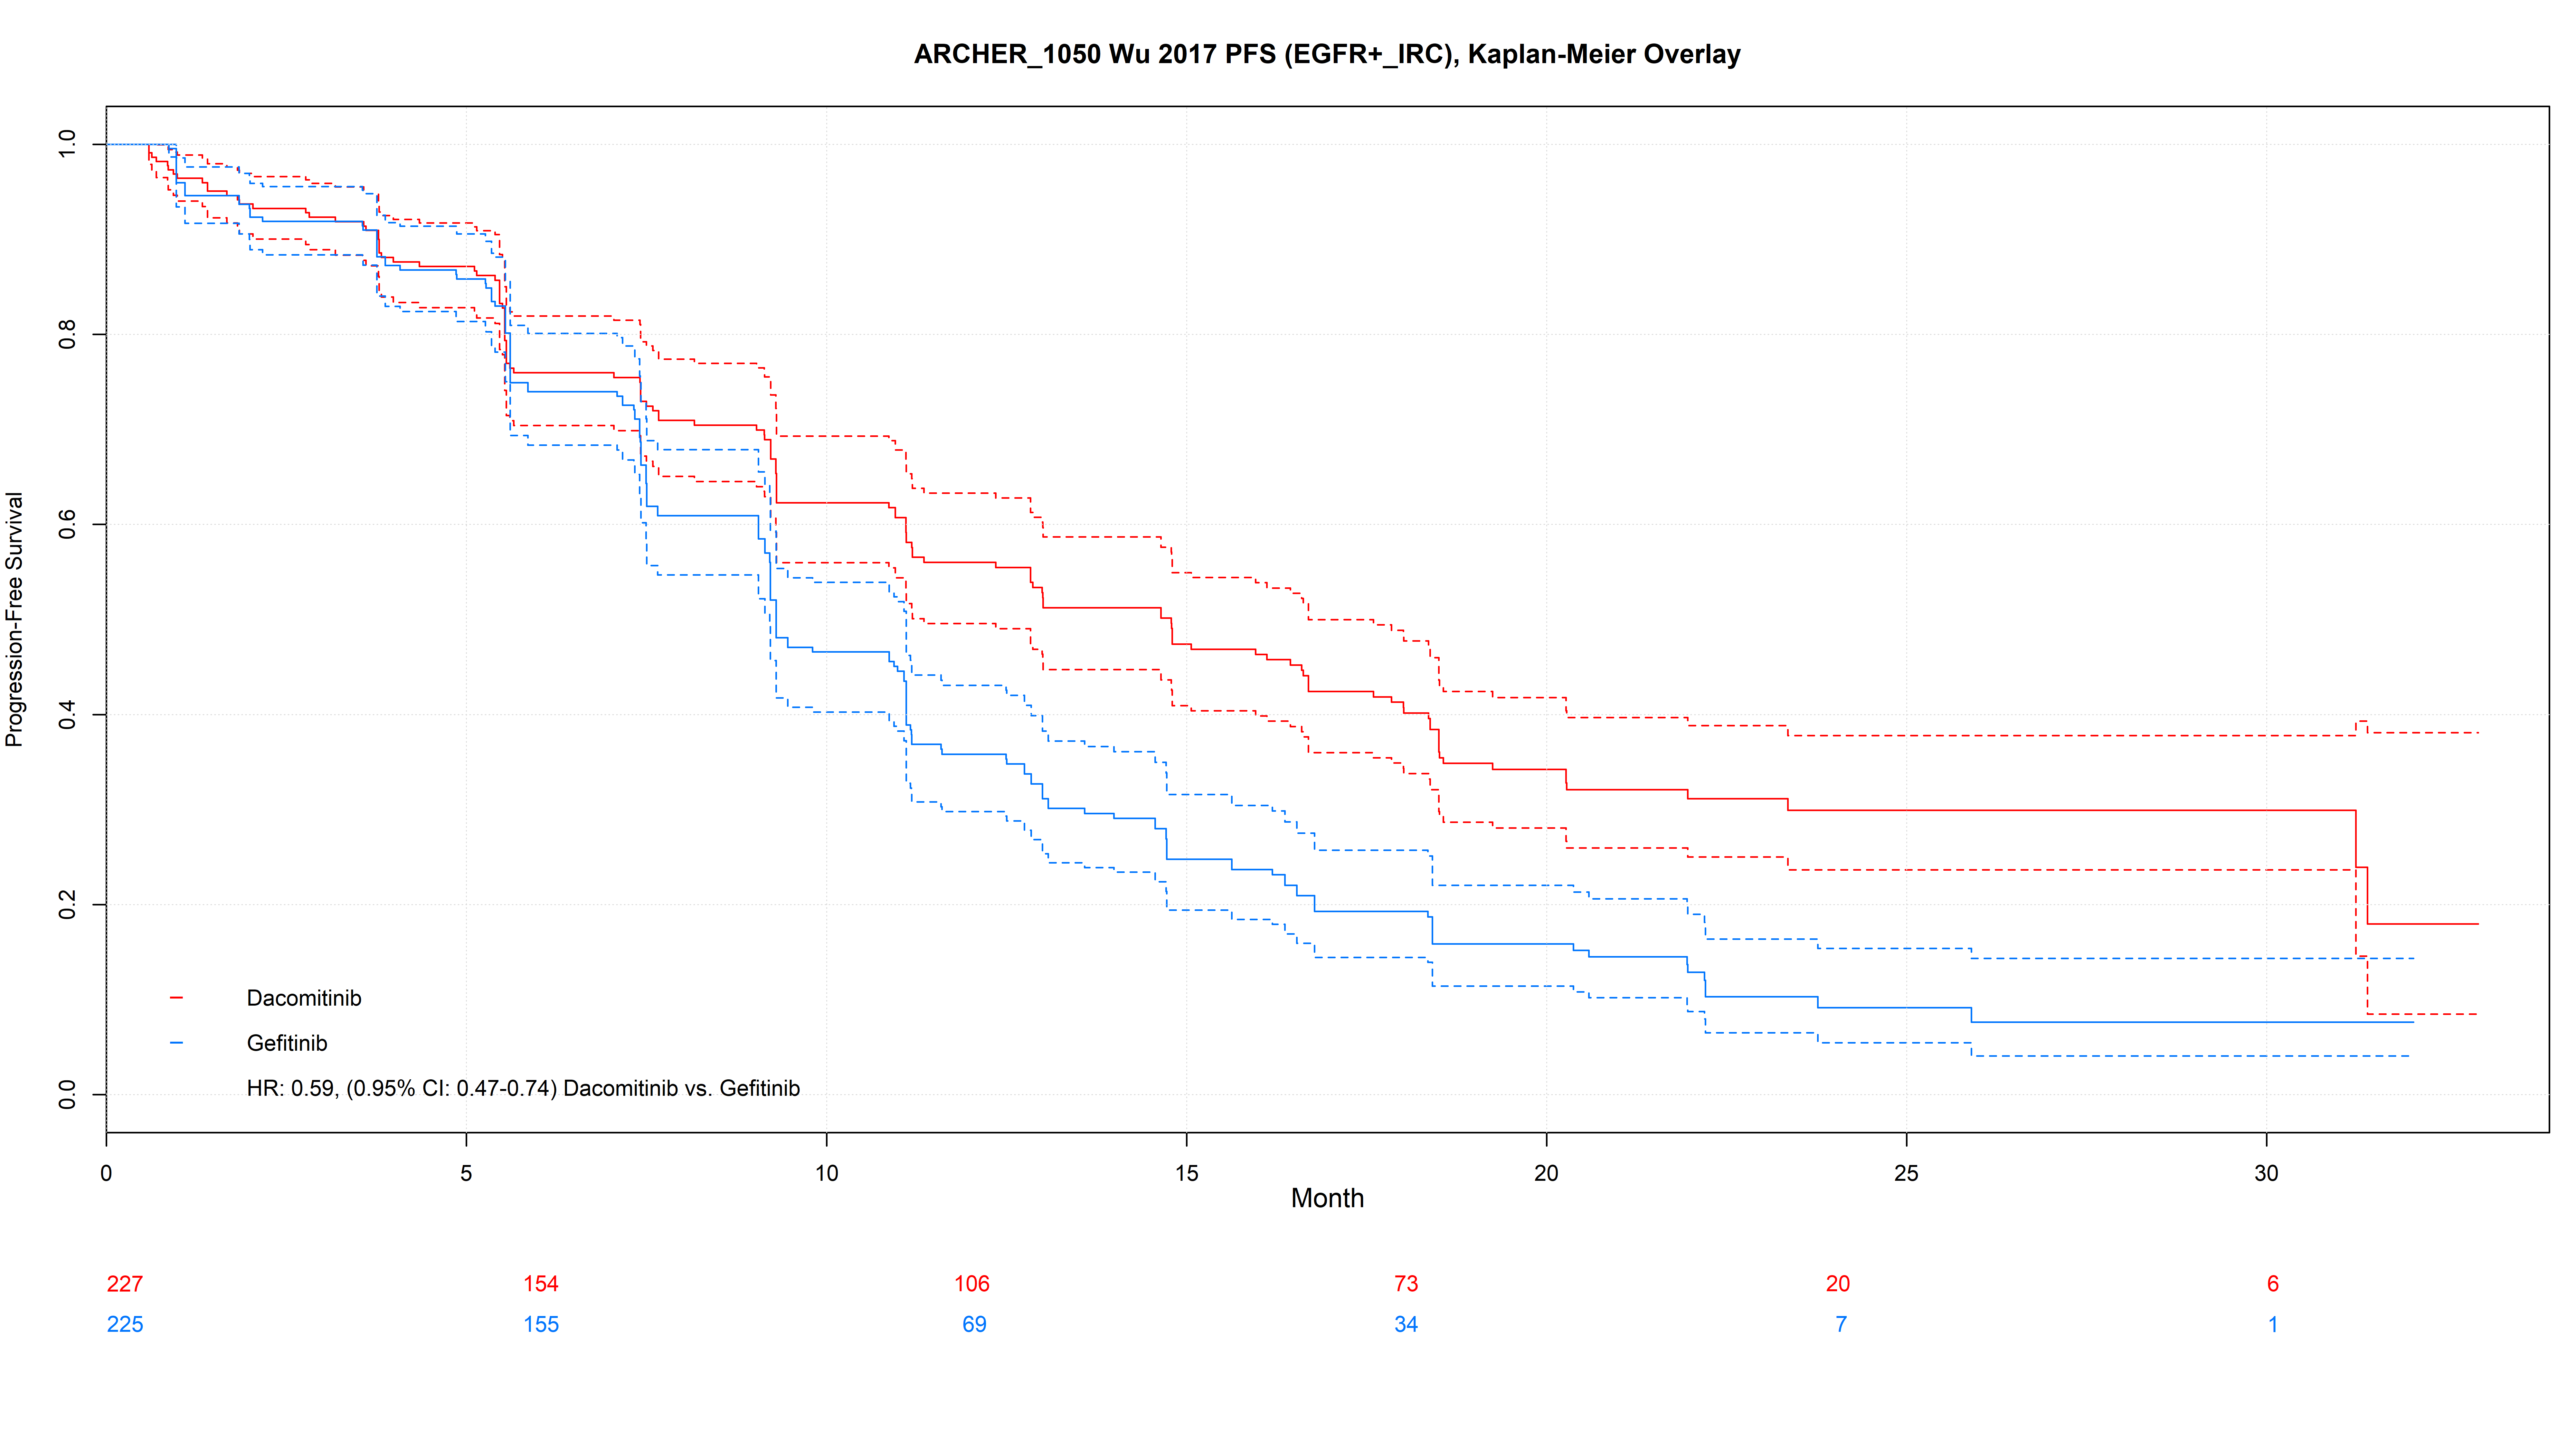
\includegraphics[max size={\textwidth}{\textheight}]{figs/km-plots/ARCHER_1050 Wu 2017 PFS (EGFR+_IRC) Kaplan Meier.png}
\end{subfigure}
\begin{subfigure}{\textwidth}
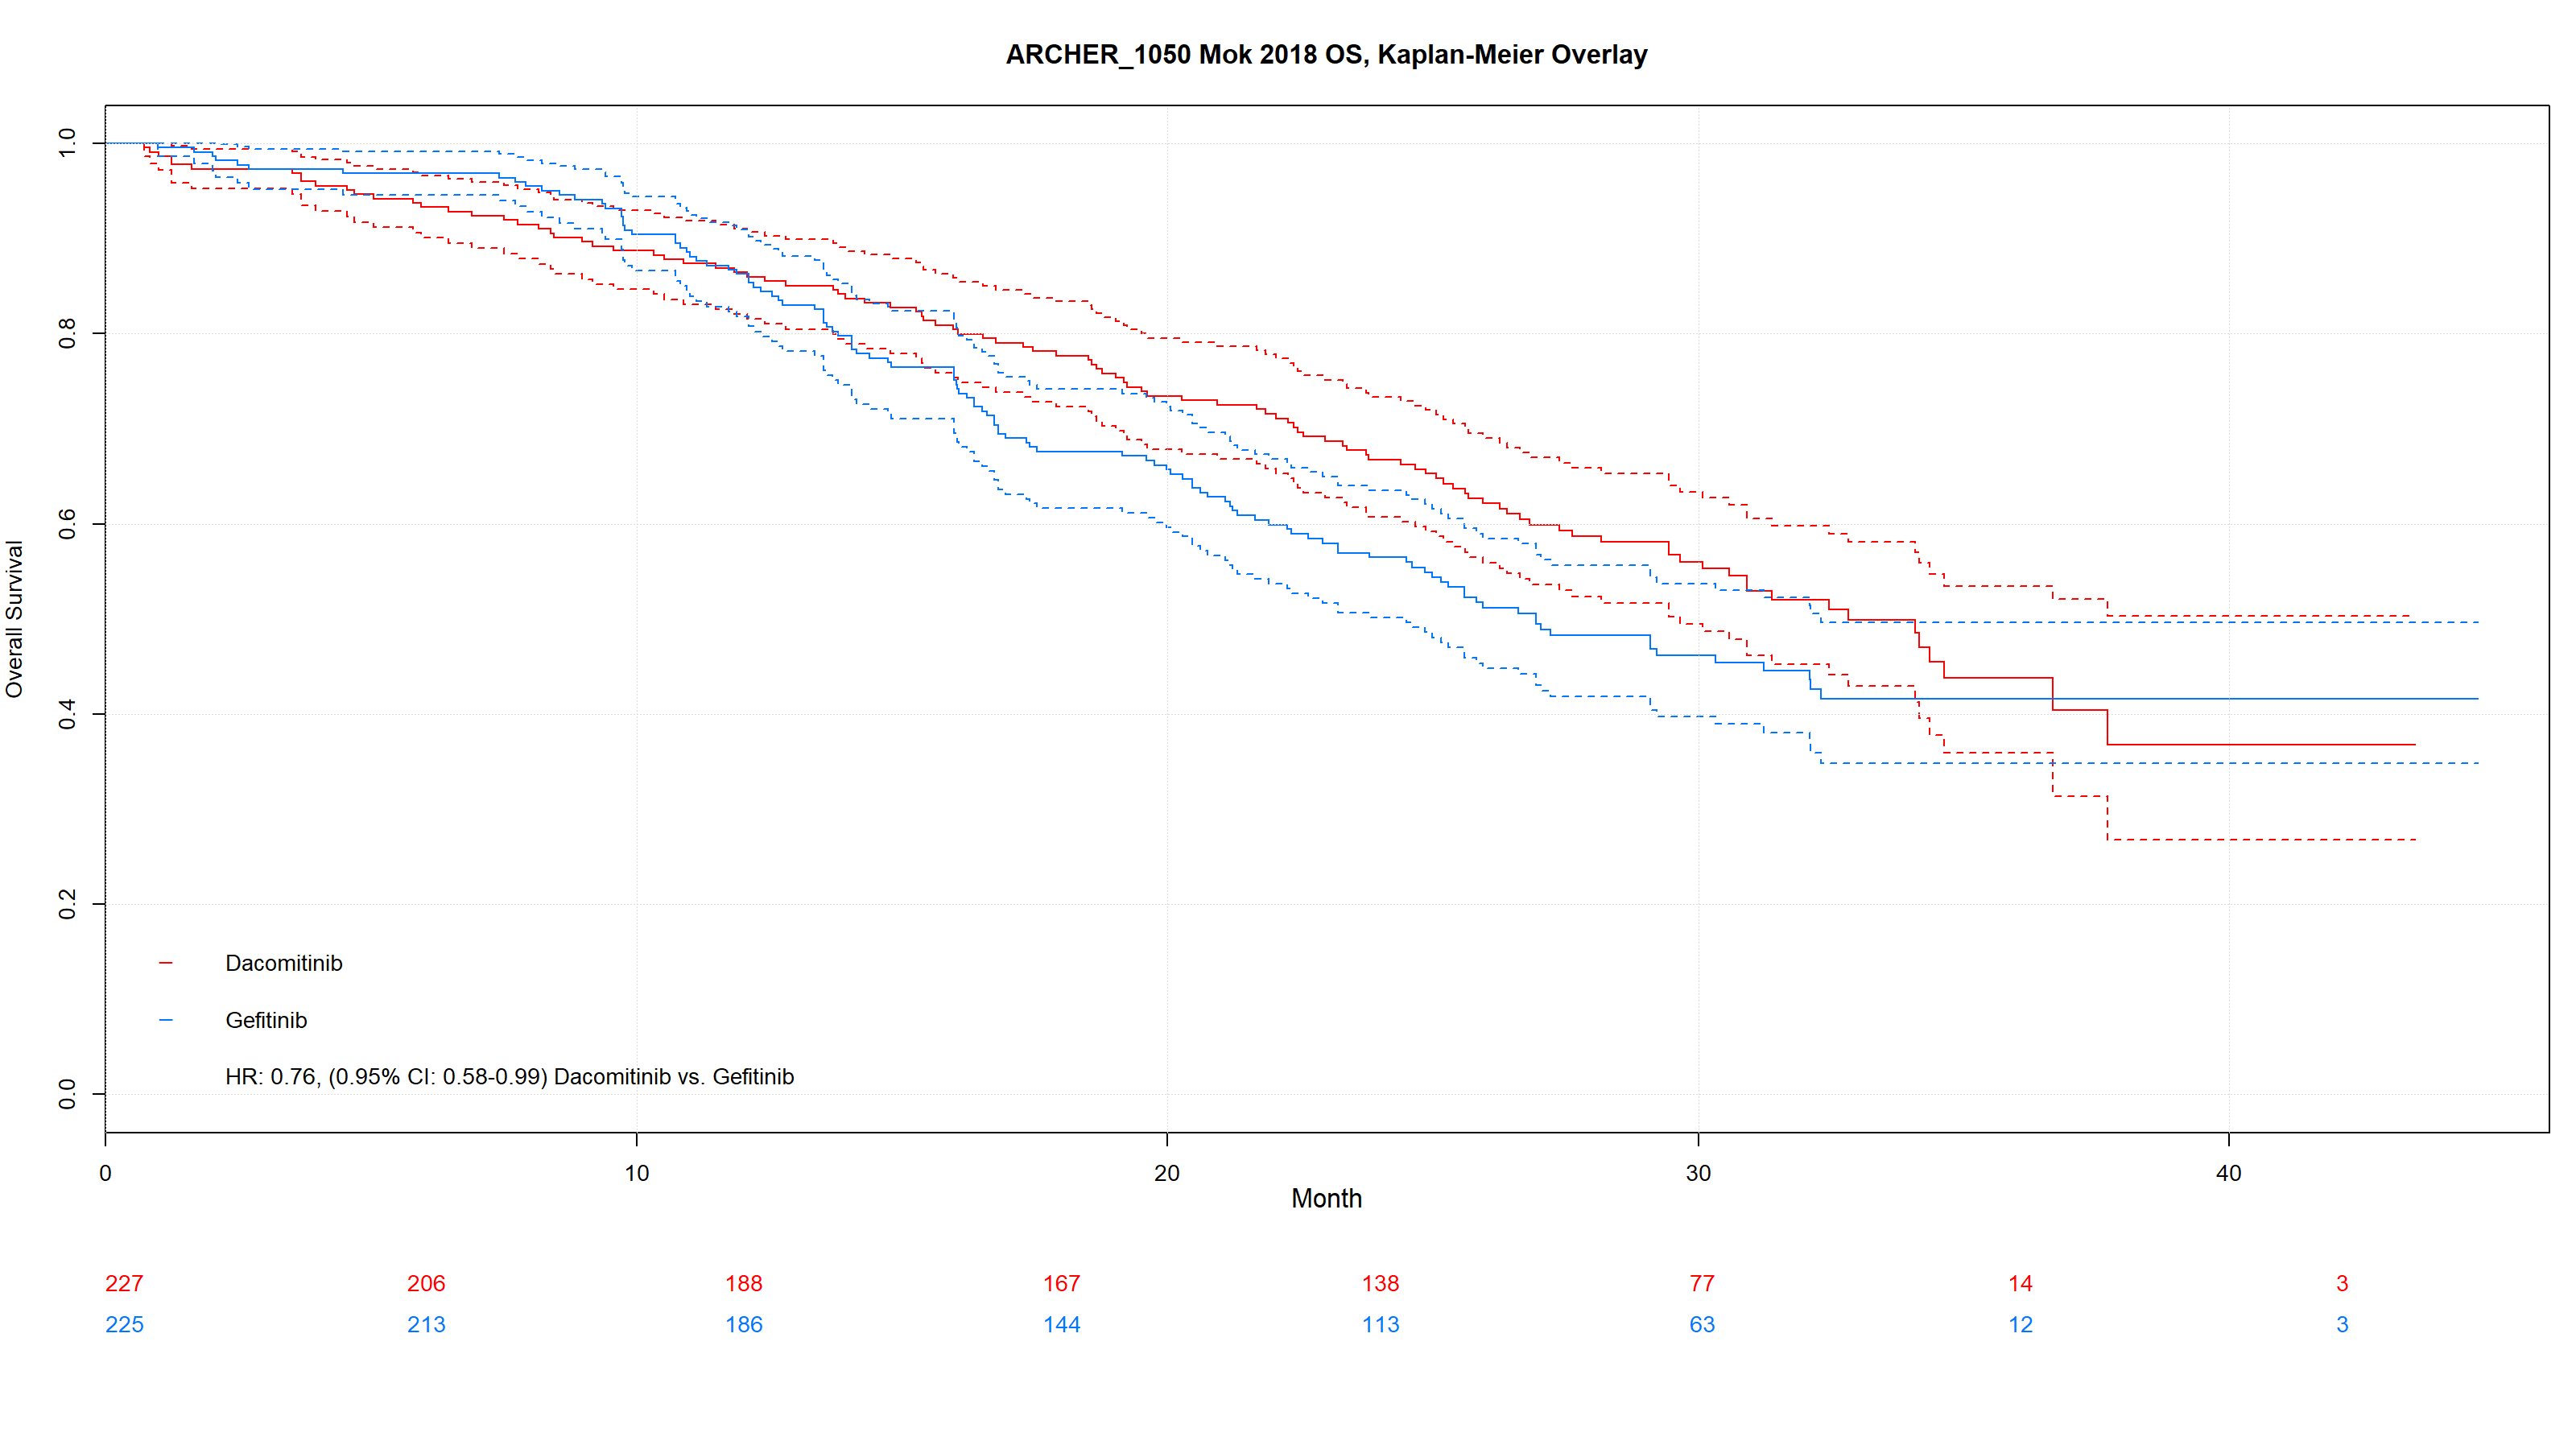
\includegraphics[max size={\textwidth}{\textheight}]{figs/km-plots/ARCHER_1050 Mok 2018 OS Kaplan Meier.png}
\end{subfigure}
\centering
\caption{ARCHER-1050, progression-free survival and overall survival}\label{fig:ARCHER-1050}
\end{figure}



\begin{figure}
\centering
\begin{subfigure}{\textwidth}
\centering
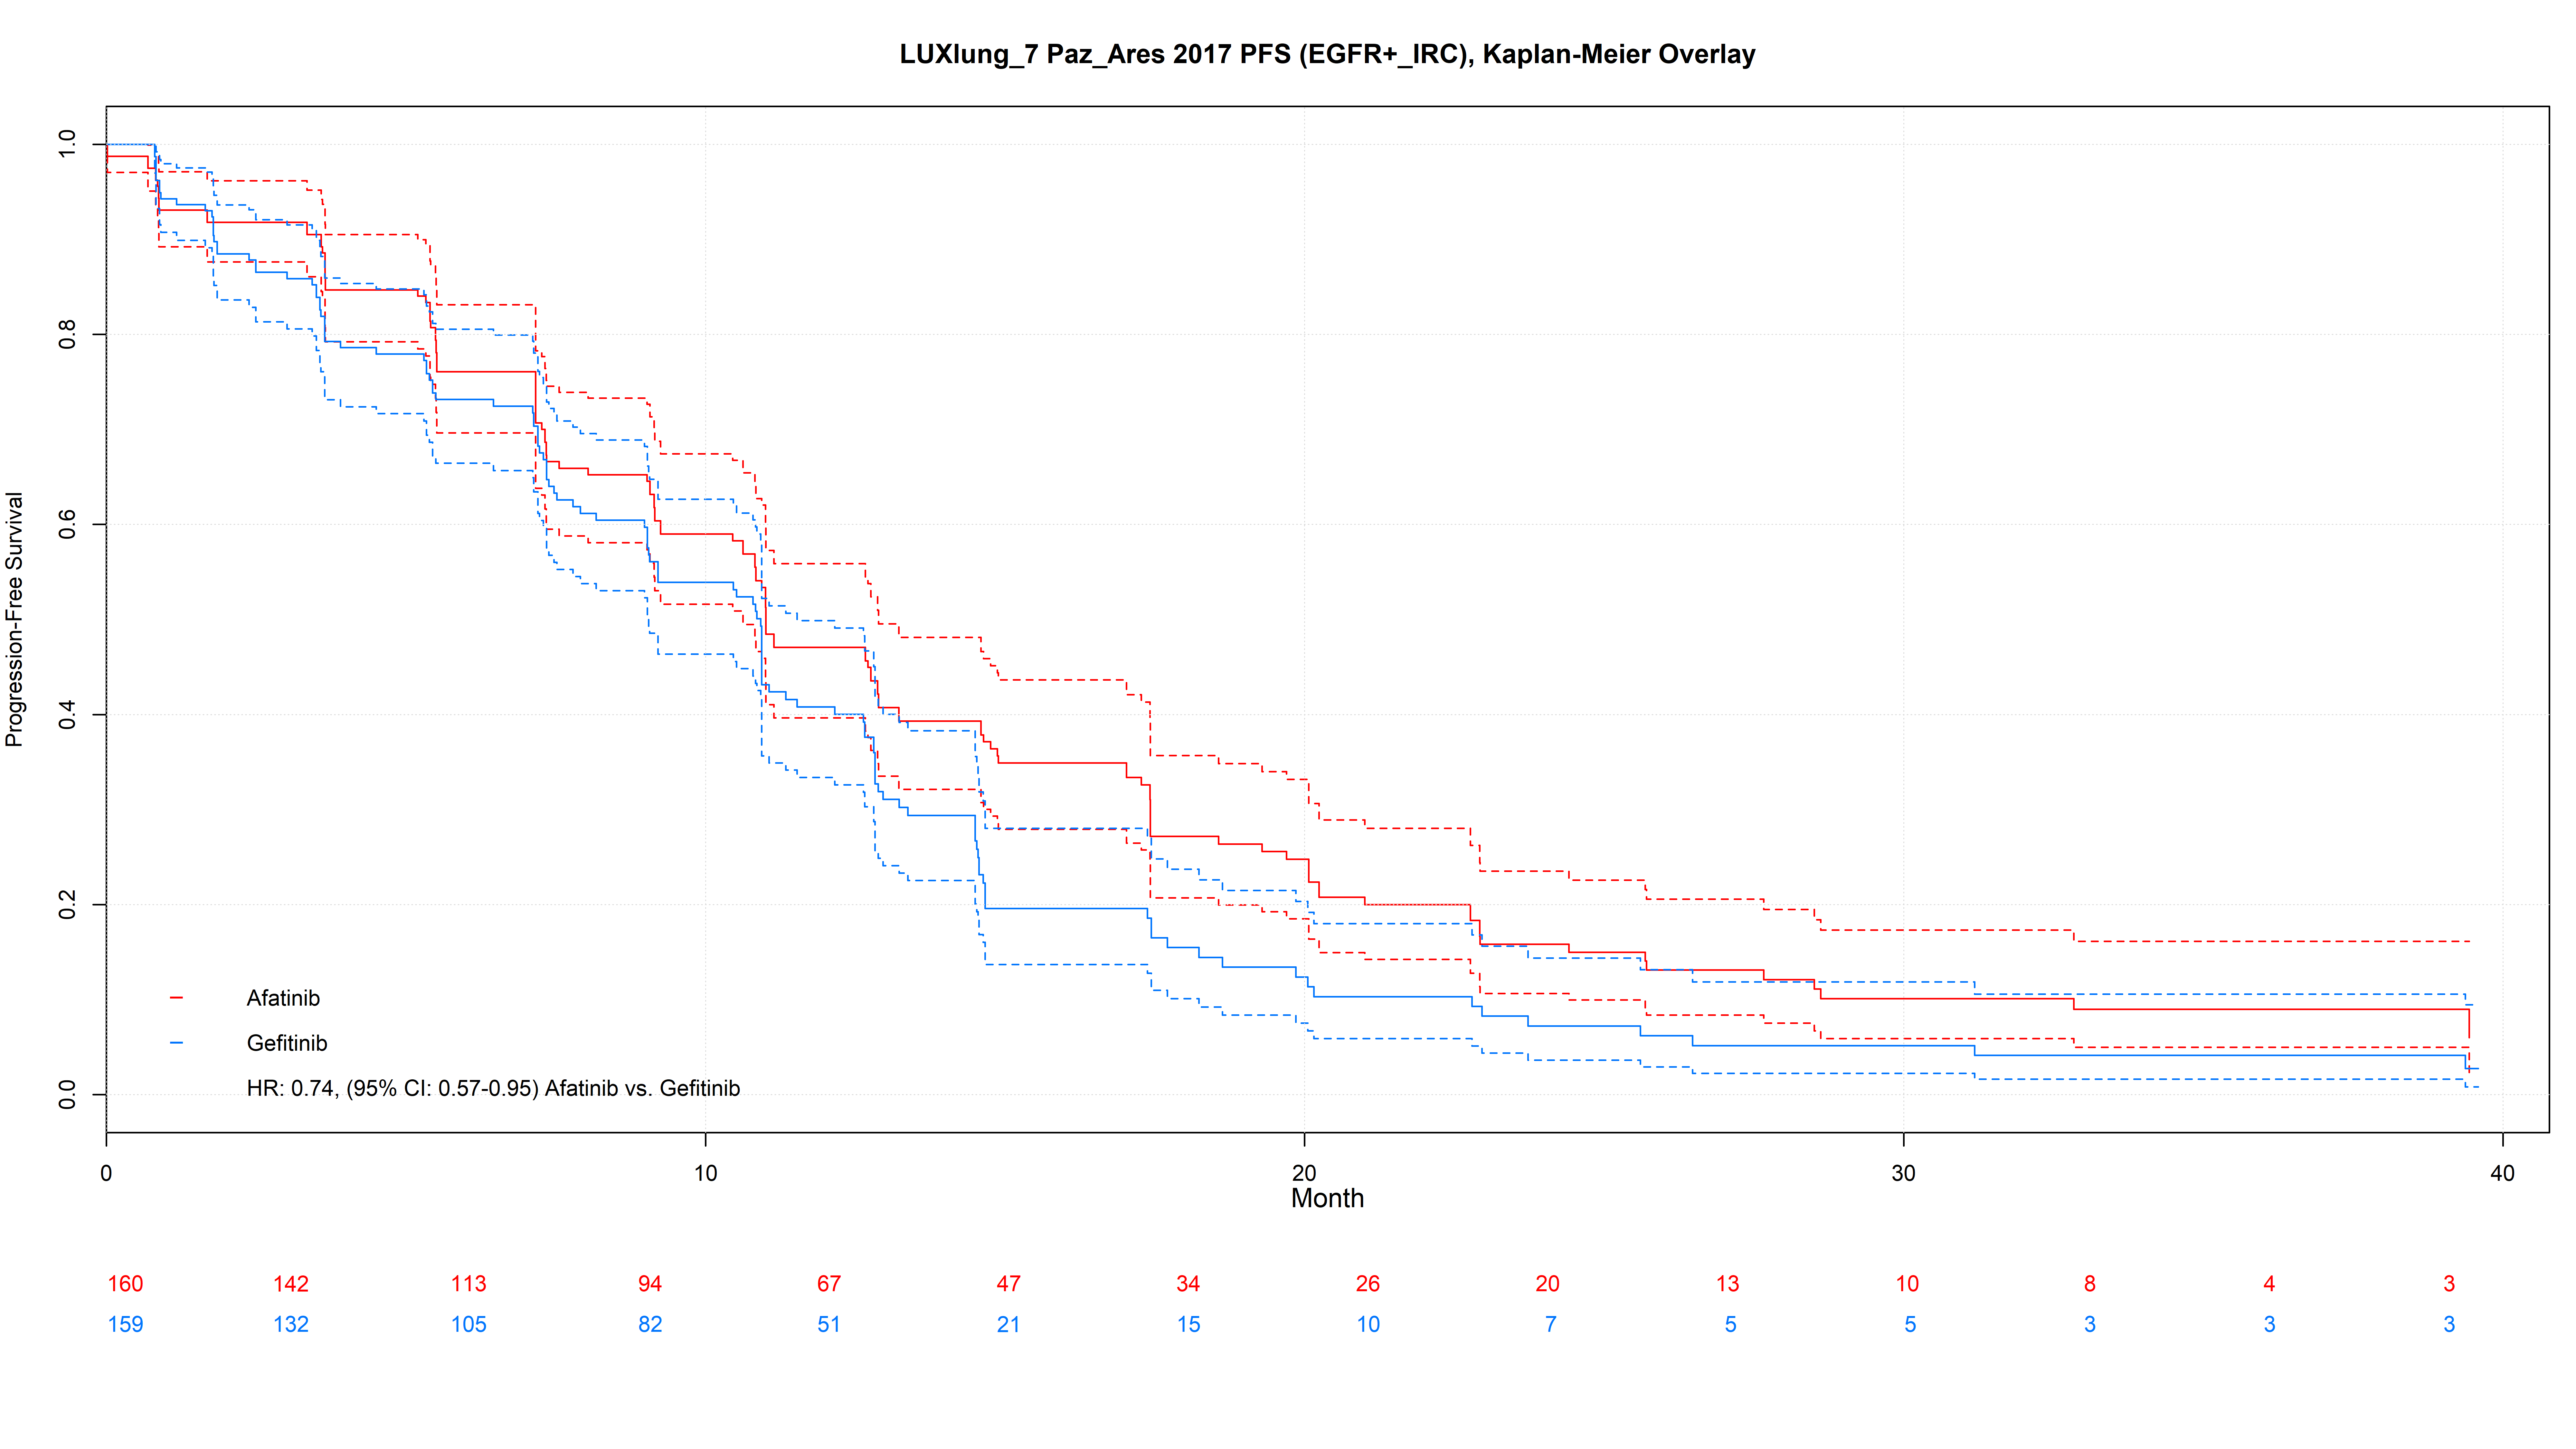
\includegraphics[max size={\textwidth}{\textheight}]{figs/km-plots/LUXlung_7 Paz_Ares 2017 PFS (EGFR+_IRC) Kaplan Meier.png}
\end{subfigure}
\begin{subfigure}{\textwidth}
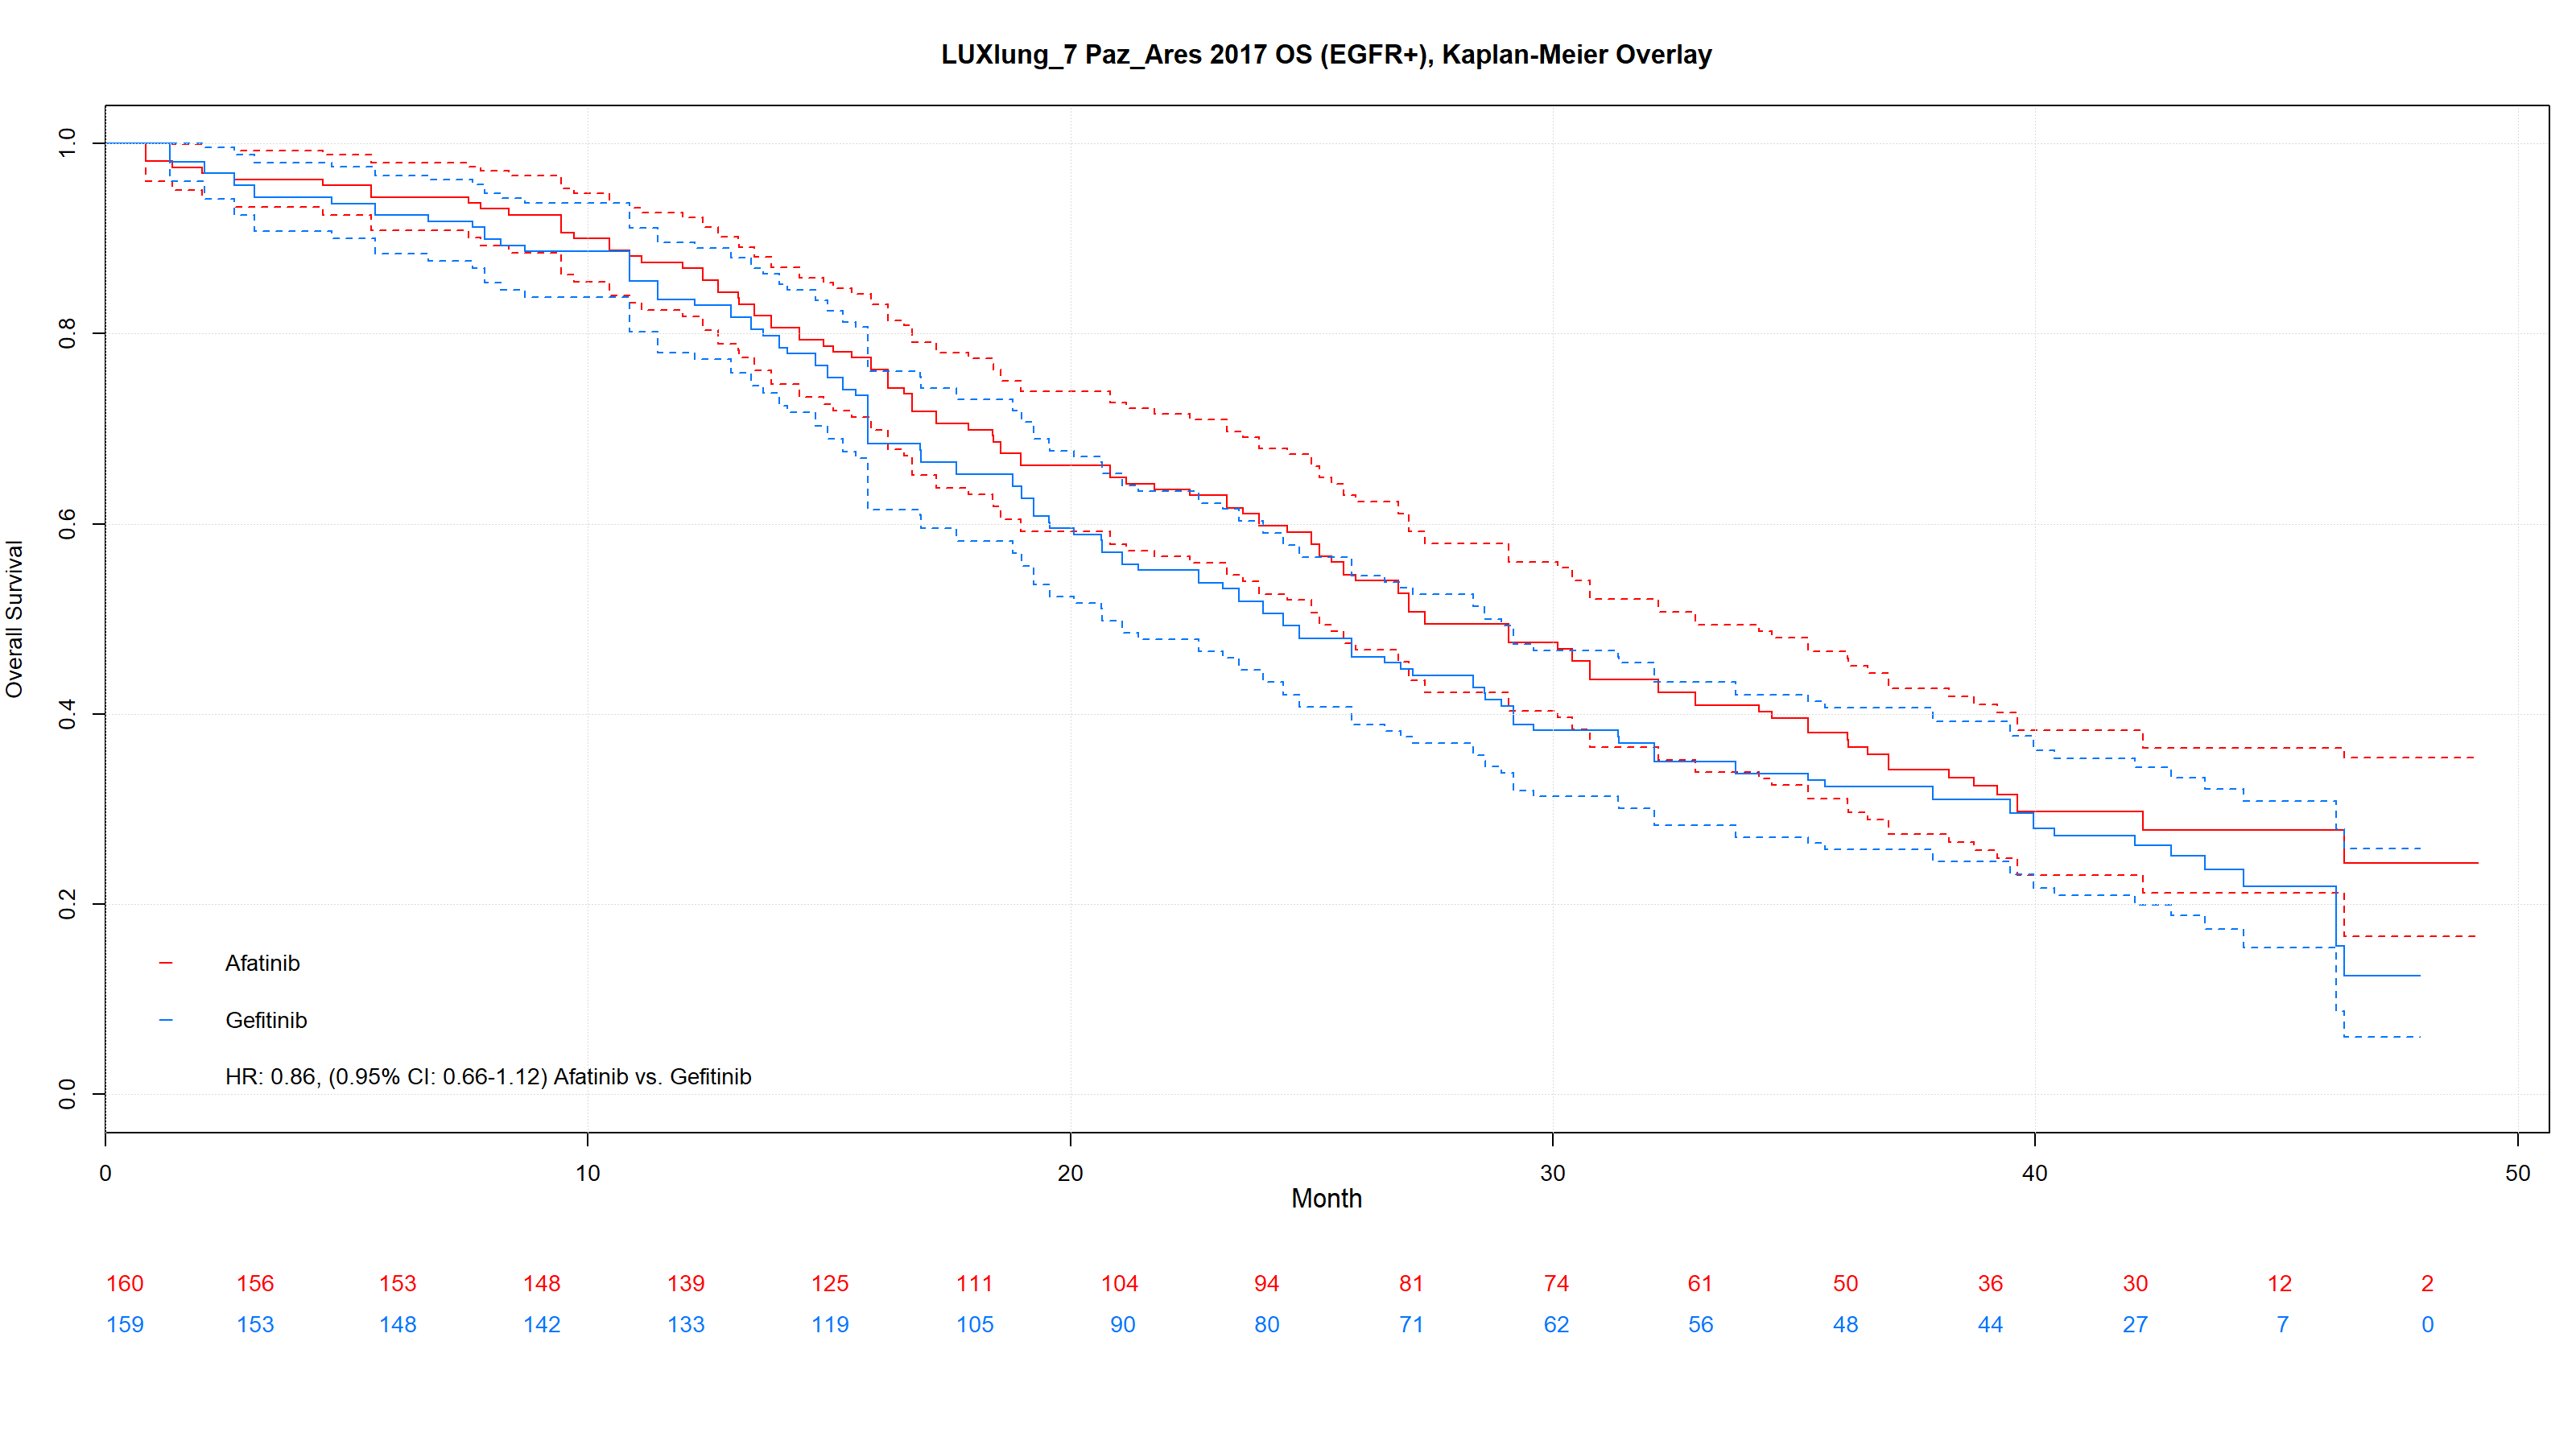
\includegraphics[max size={\textwidth}{\textheight}]{figs/km-plots/LUXlung_7 Paz_Ares 2017 OS (EGFR+) Kaplan Meier.png}
\end{subfigure}
\centering
\caption{LUX-LUNG 7, progression-free survival and overall survival}\label{fig:LUX-LUNG 7}
\end{figure}


\begin{figure}
\centering
\begin{subfigure}{\textwidth}
\centering
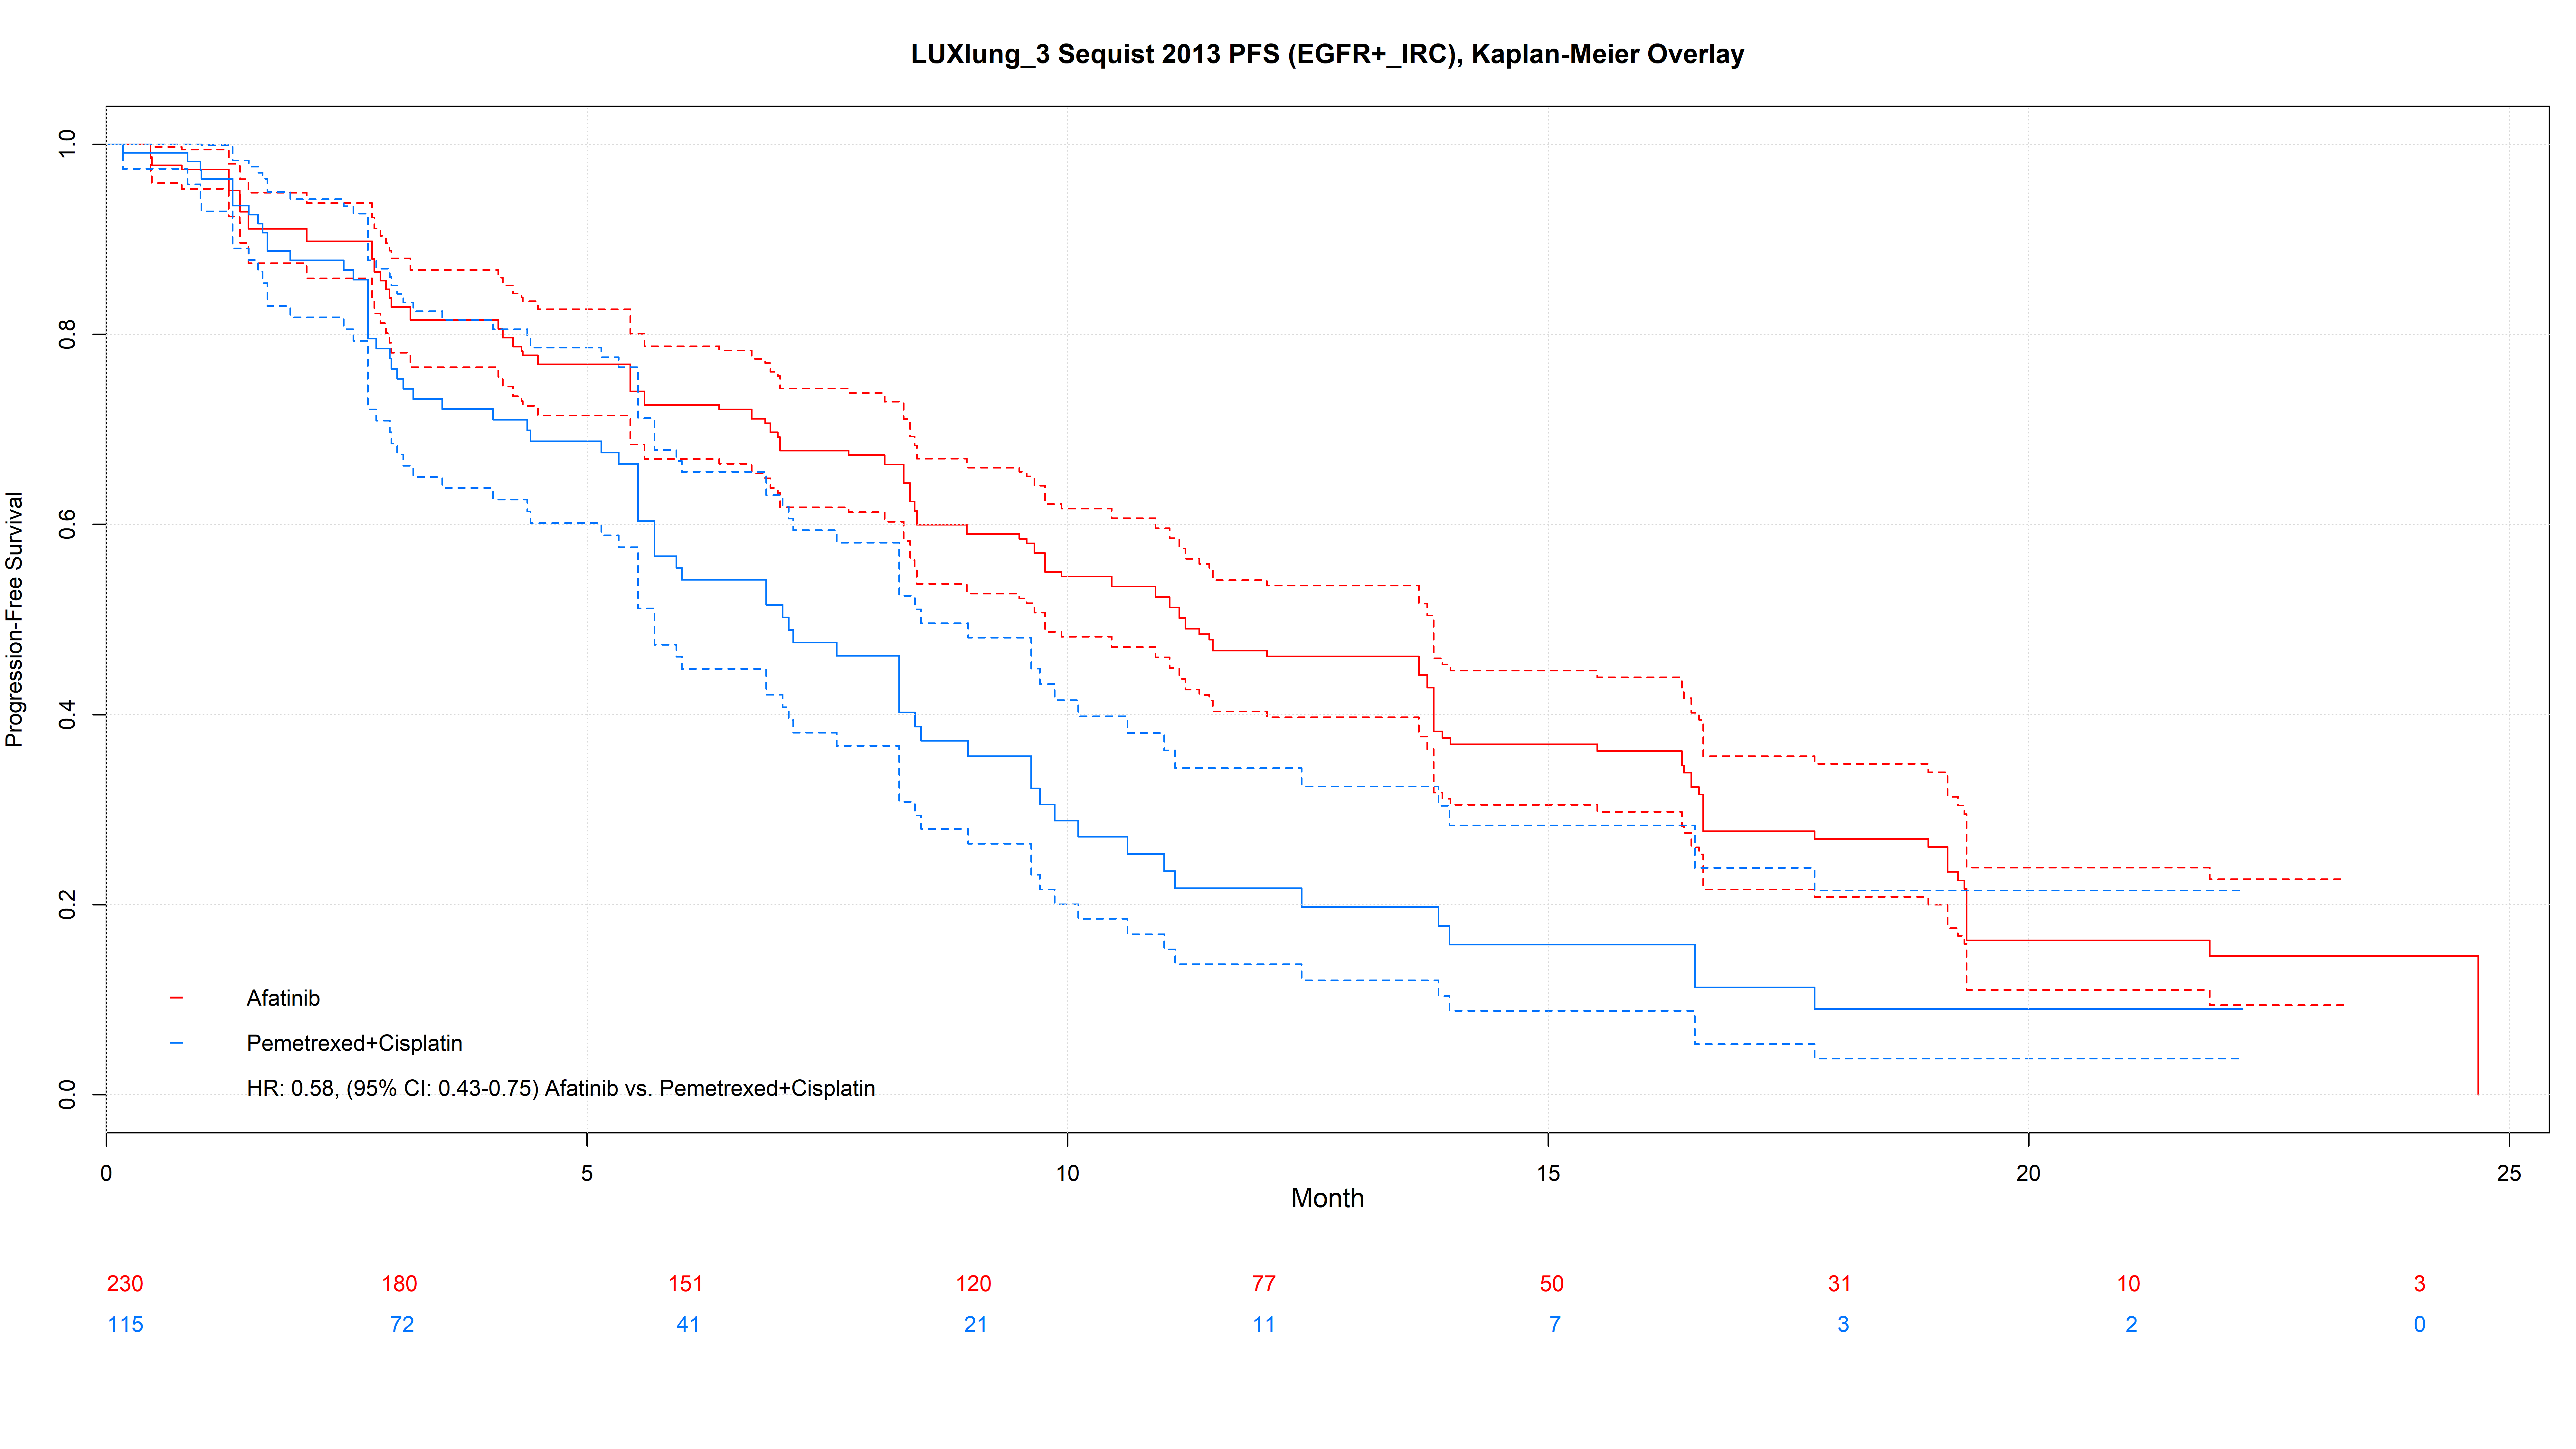
\includegraphics[max size={\textwidth}{\textheight}]{figs/km-plots/LUXlung_3 Sequist 2013 PFS (EGFR+_IRC) Kaplan Meier.png}
\end{subfigure}
\begin{subfigure}{\textwidth}
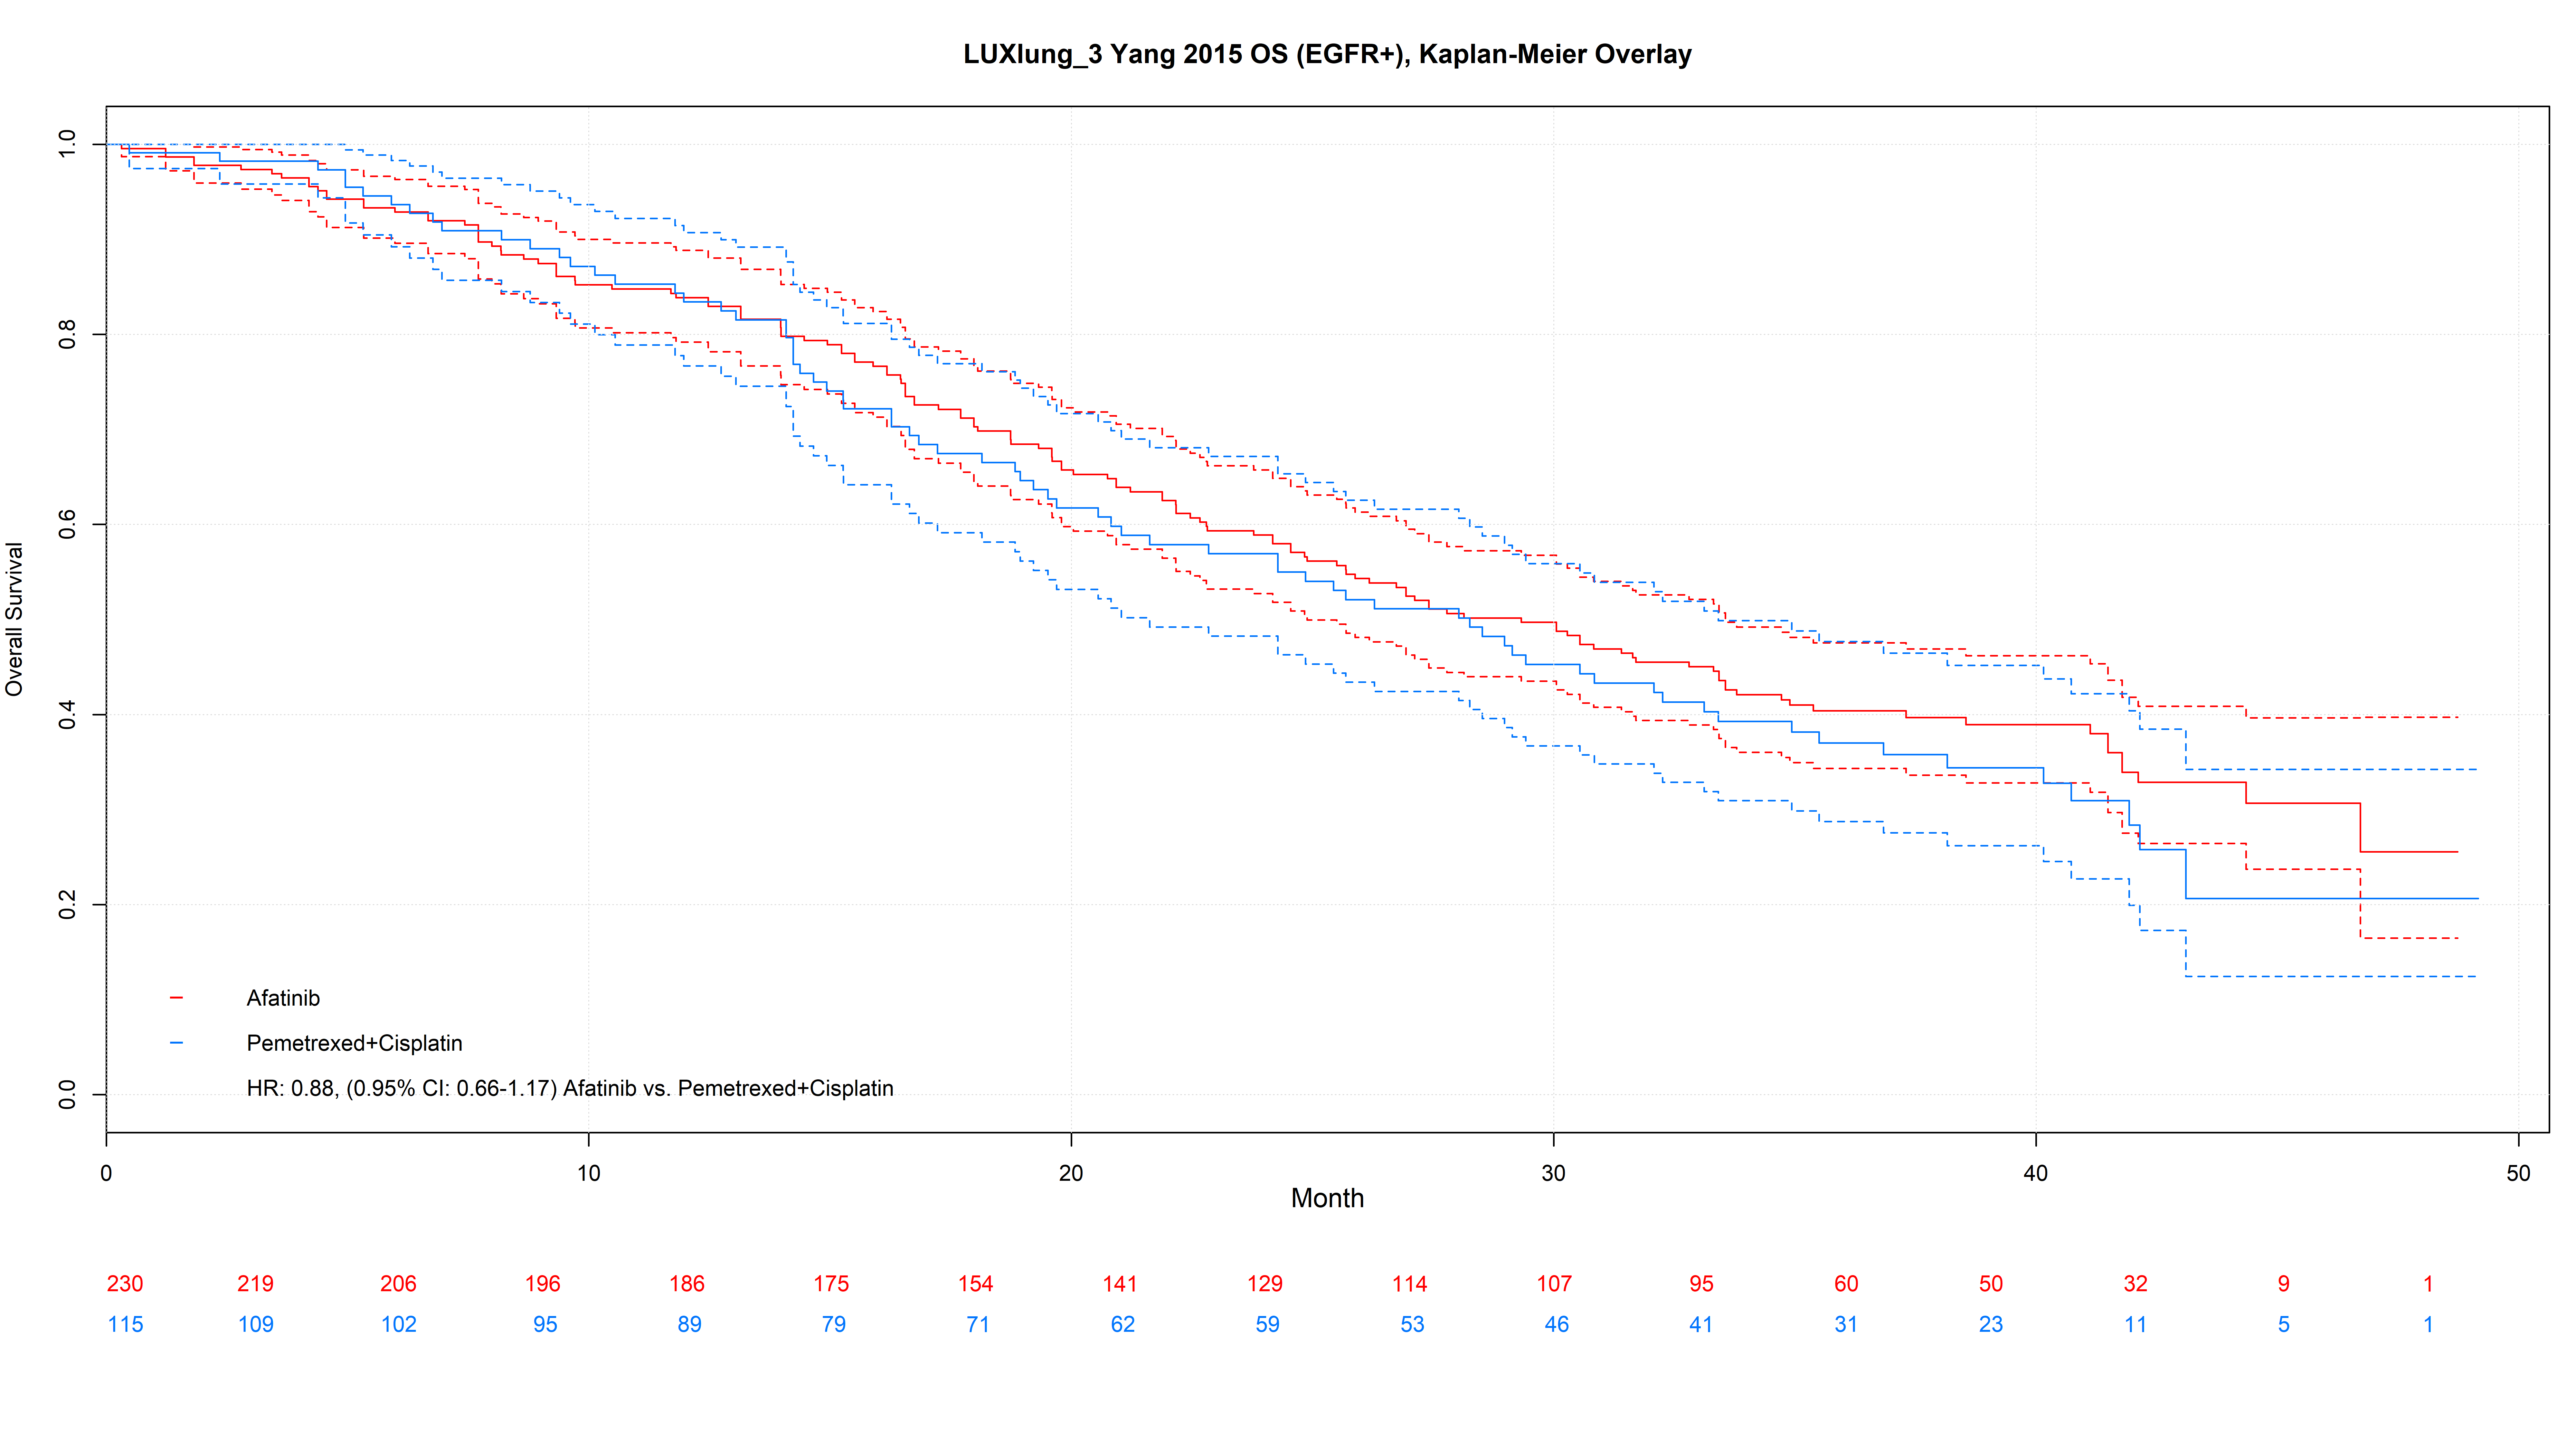
\includegraphics[max size={\textwidth}{\textheight}]{figs/km-plots/LUXlung_3 Yang 2015 OS (EGFR+) Kaplan Meier.png}
\end{subfigure}
\centering
\caption{LUX-LUNG 3, progression-free survival and overall survival}\label{fig:LUX-LUNG 3}
\end{figure}


\begin{figure}
\centering
\begin{subfigure}{\textwidth}
\centering
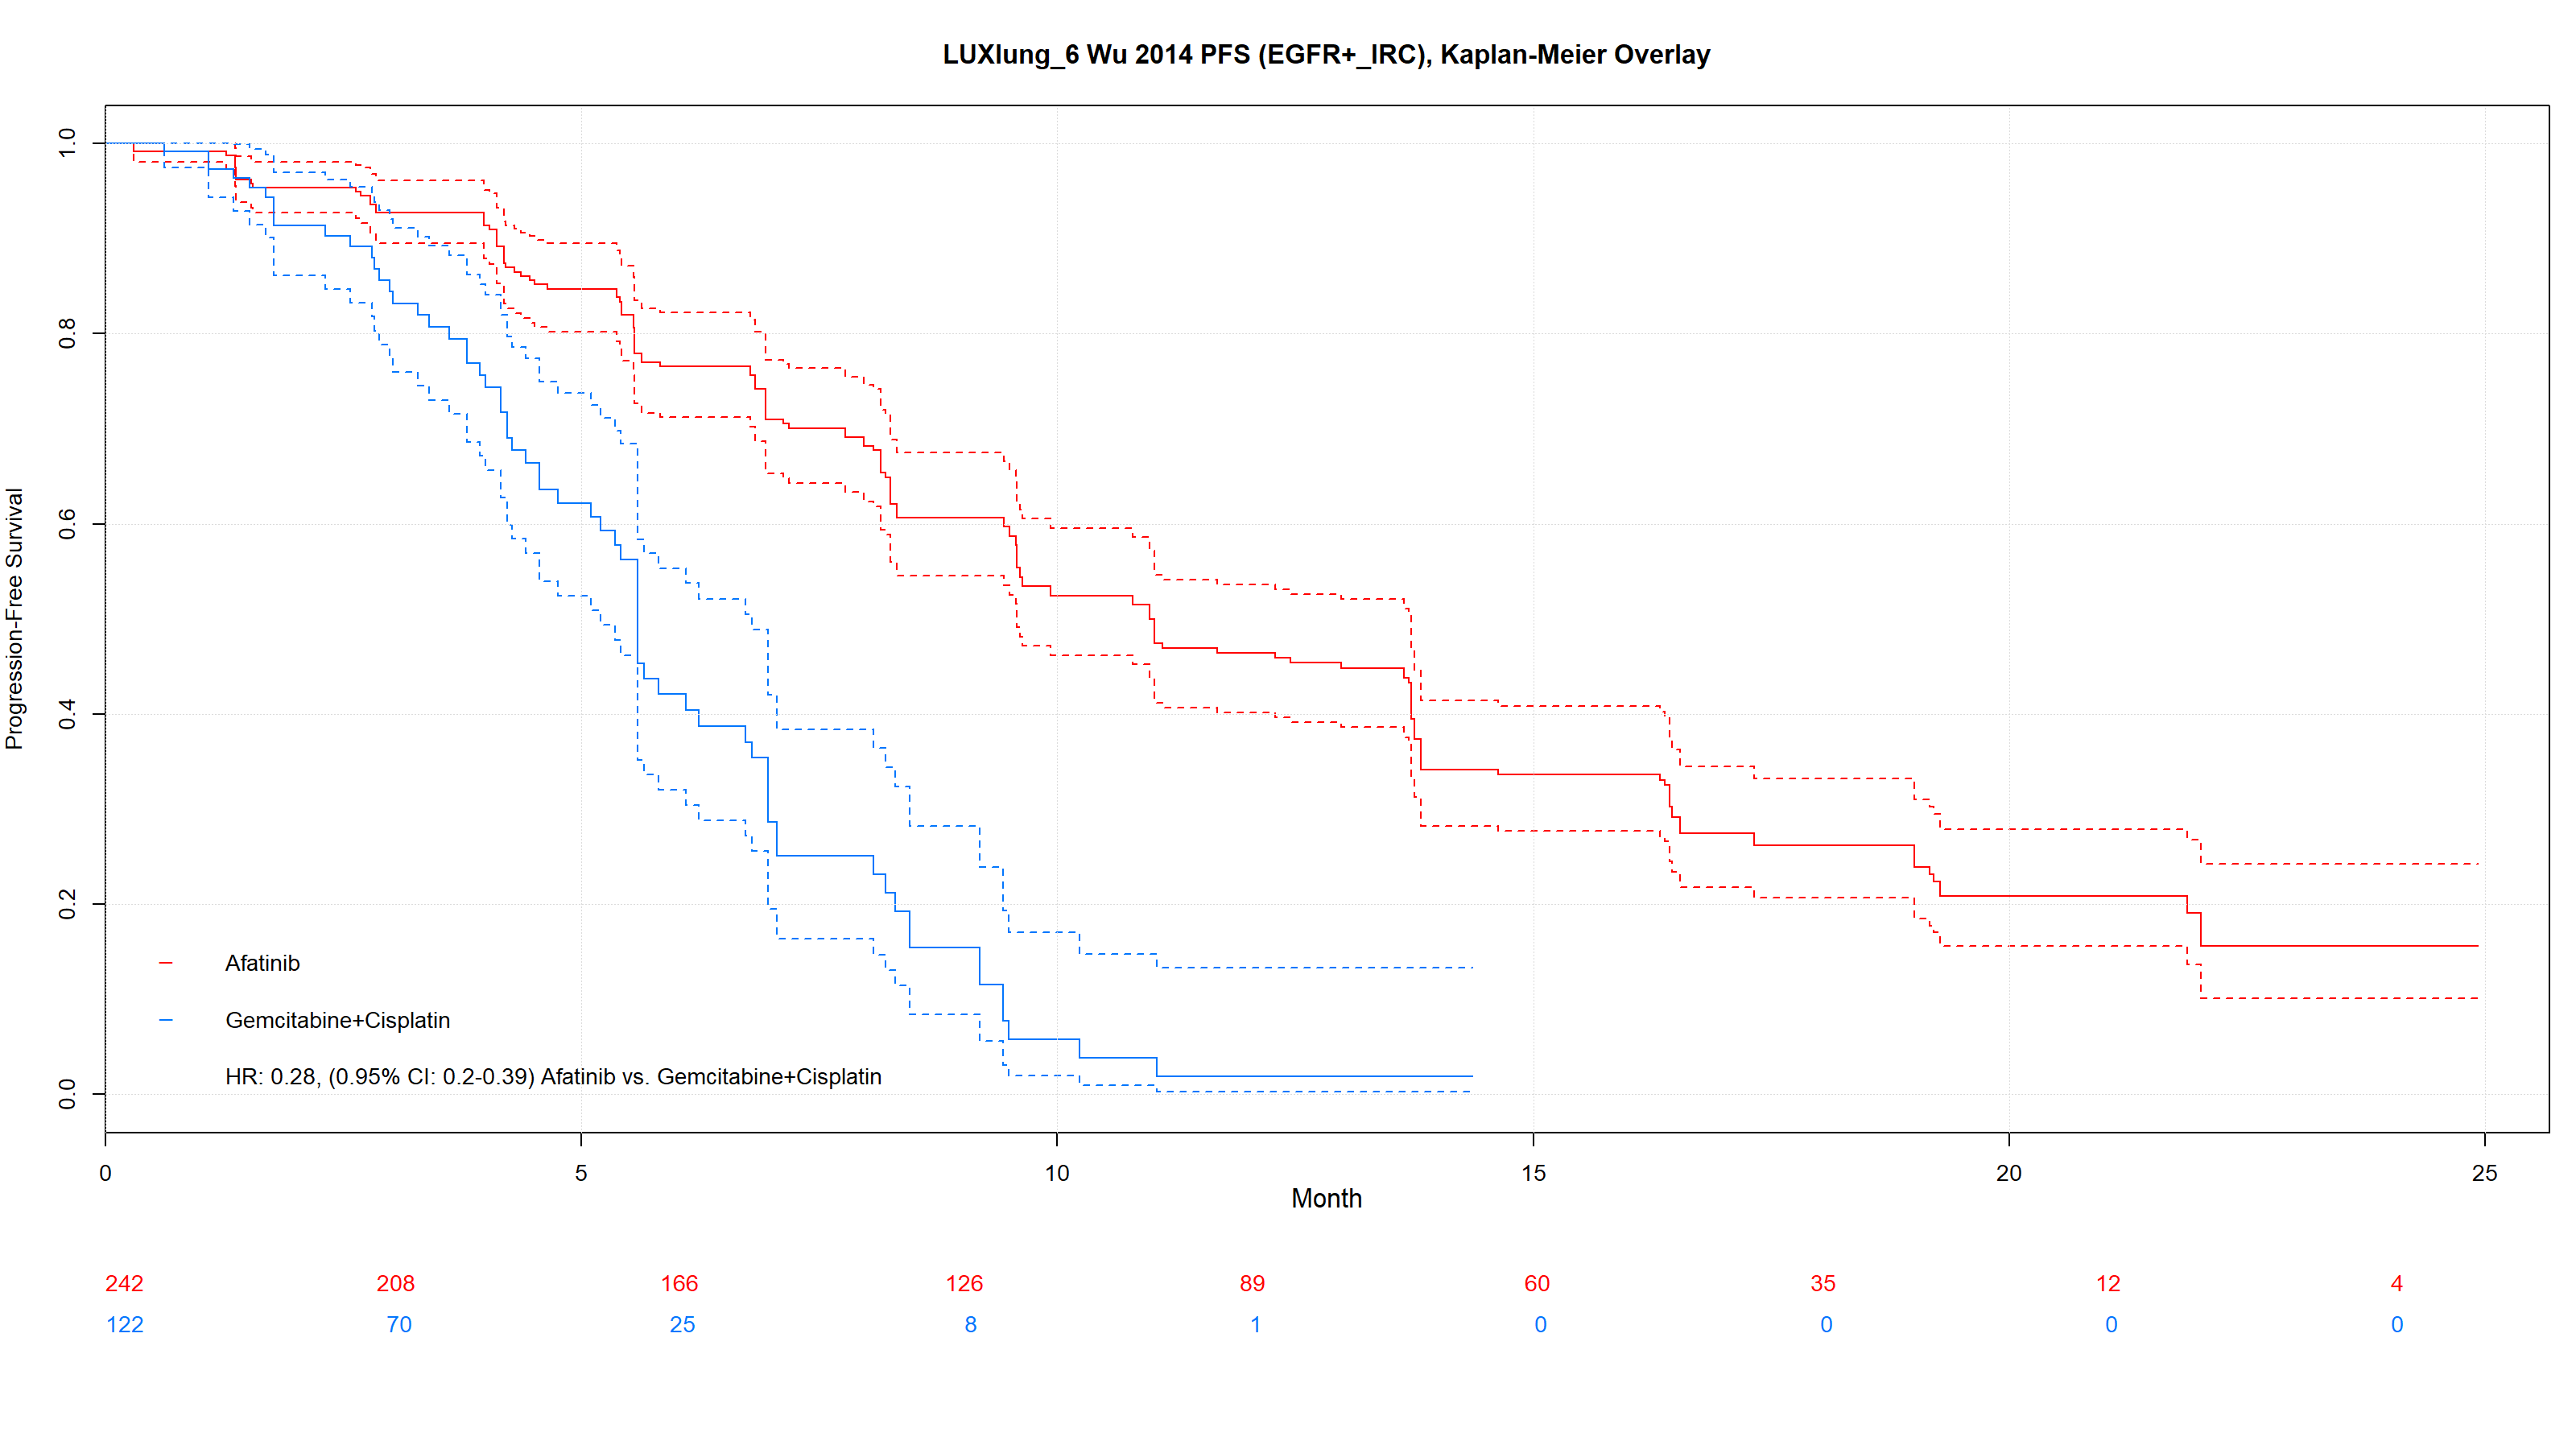
\includegraphics[max size={\textwidth}{\textheight}]{figs/km-plots/LUXlung_6 Wu 2014 PFS (EGFR+_IRC) Kaplan Meier.png}
\end{subfigure}
\begin{subfigure}{\textwidth}
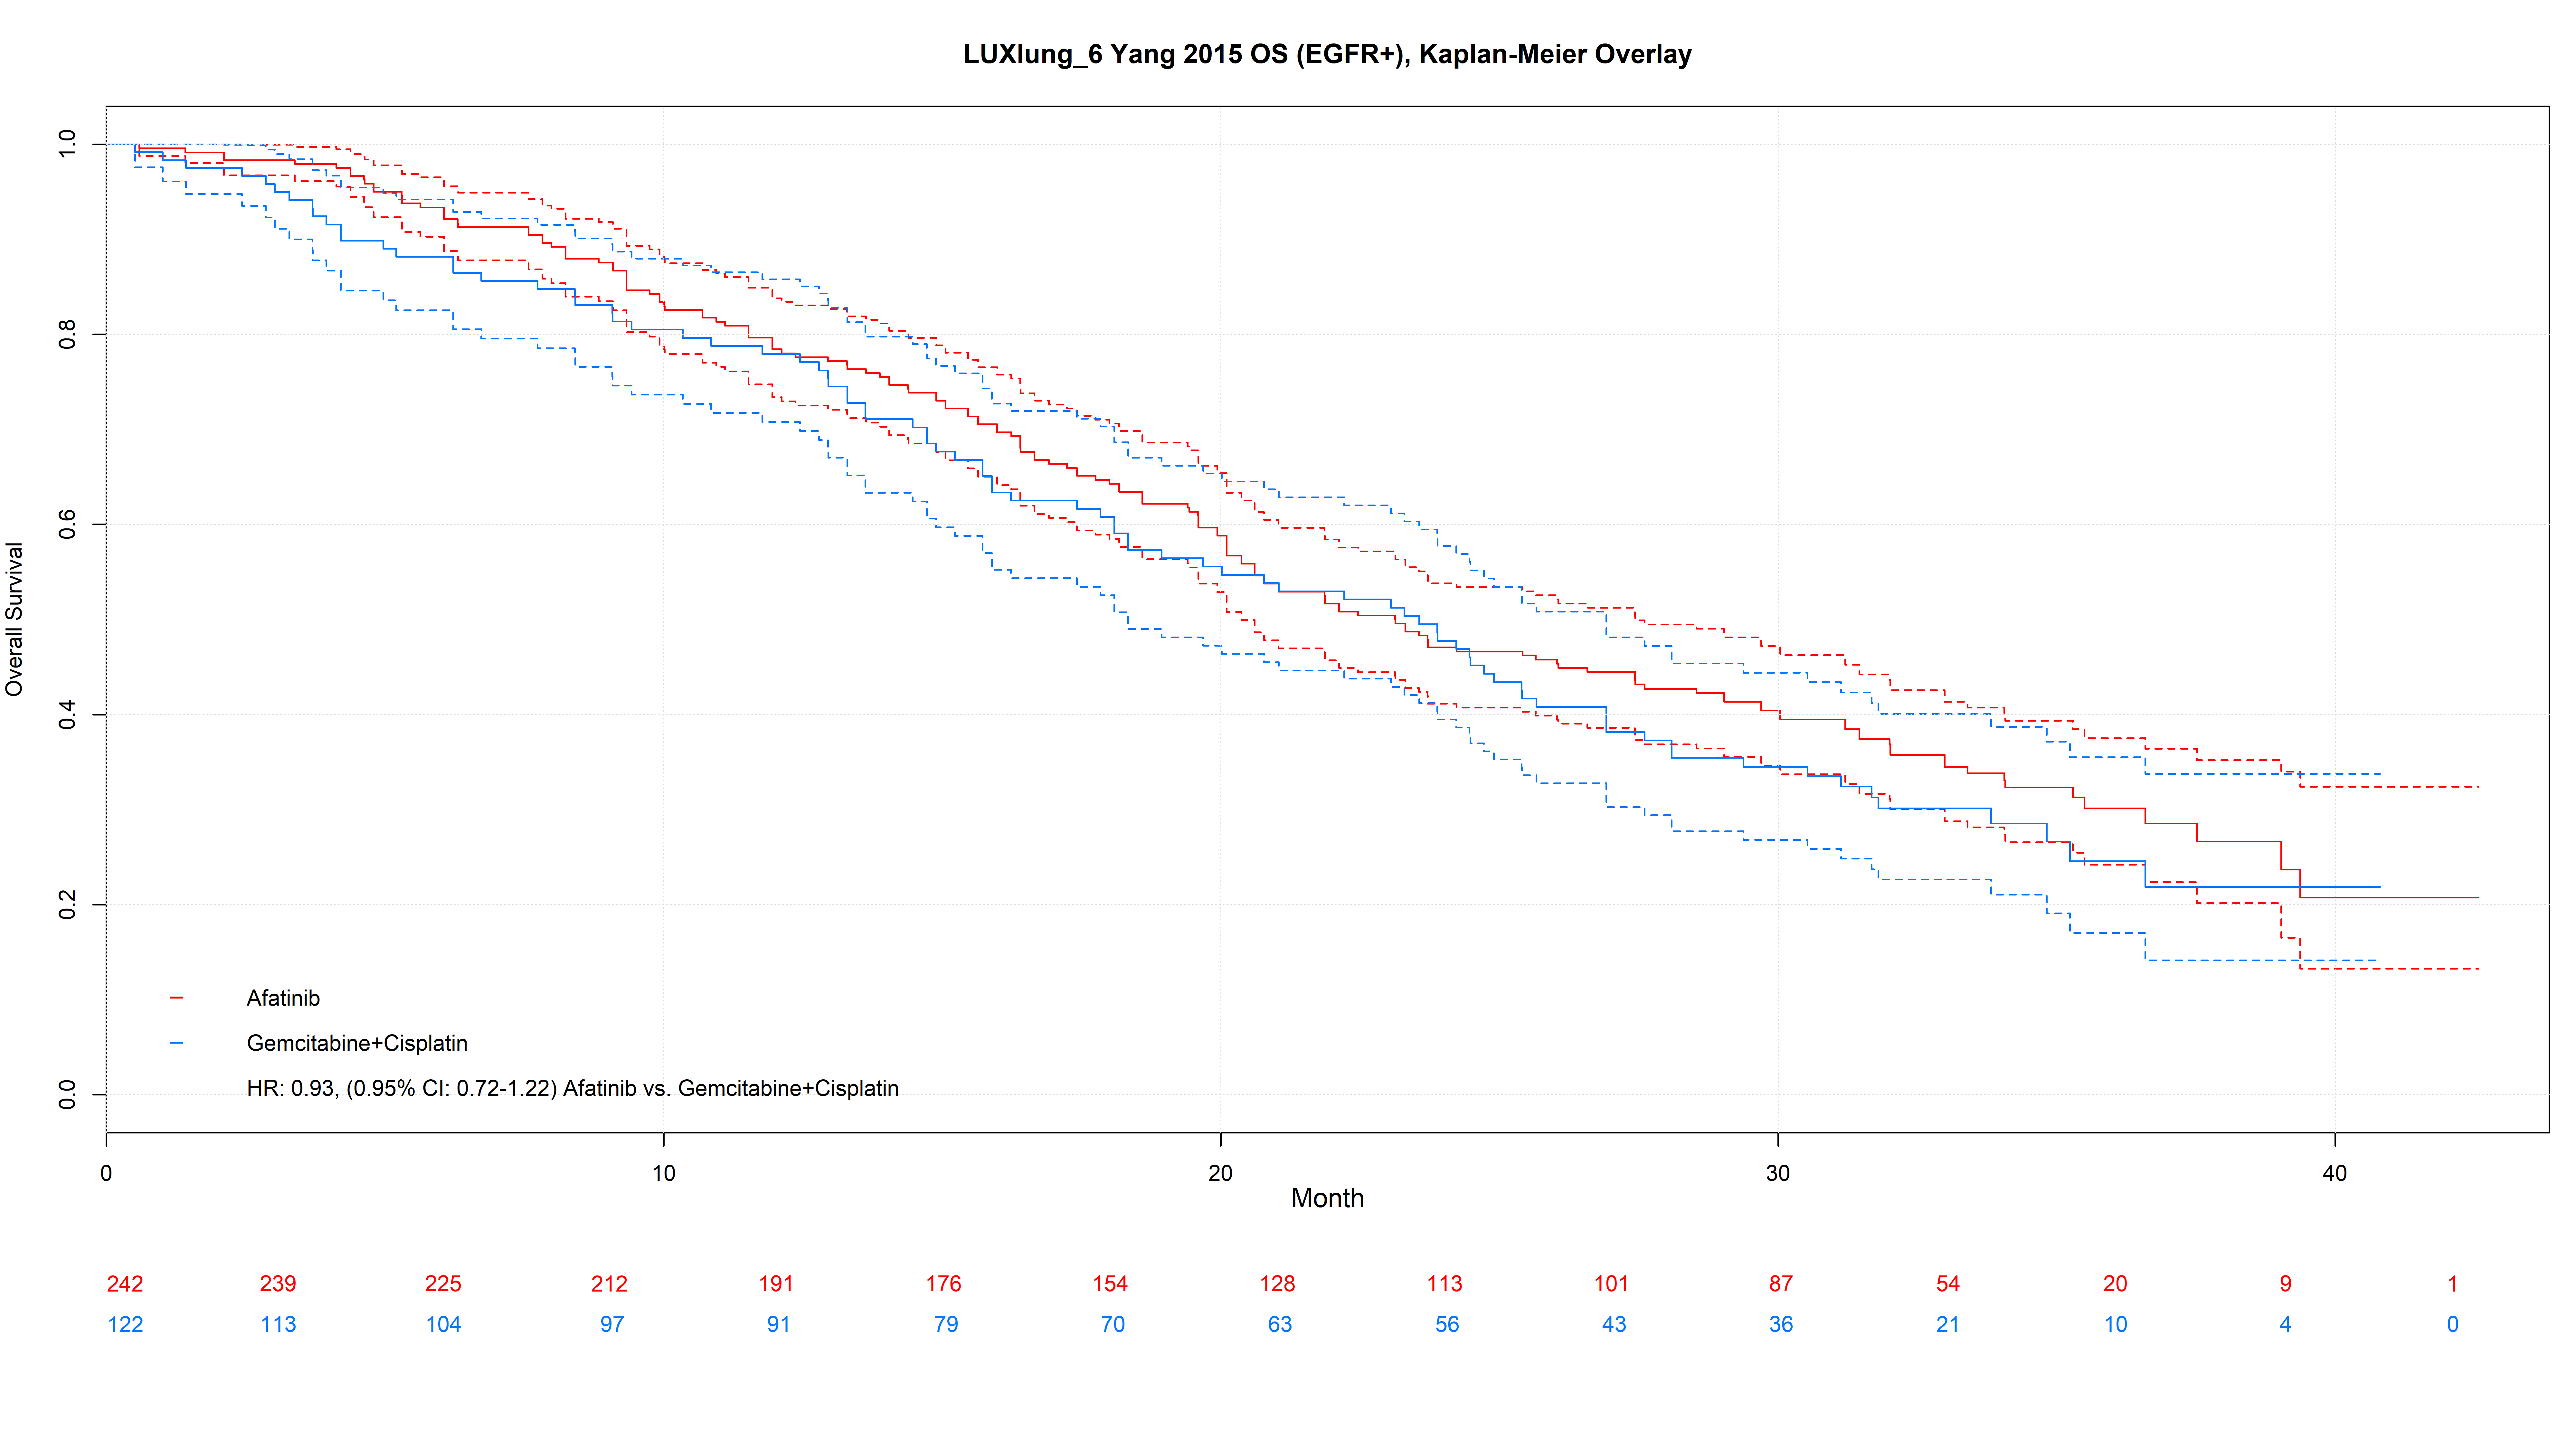
\includegraphics[max size={\textwidth}{\textheight}]{figs/km-plots/LUXlung_6 Yang 2015 OS (EGFR+) Kaplan Meier.png}
\end{subfigure}
\centering
\caption{LUX-LUNG 6, progression-free survival and overall survival}\label{fig:LUX-LUNG 6}
\end{figure}

\begin{figure}
\centering
\begin{subfigure}{\textwidth}
\centering
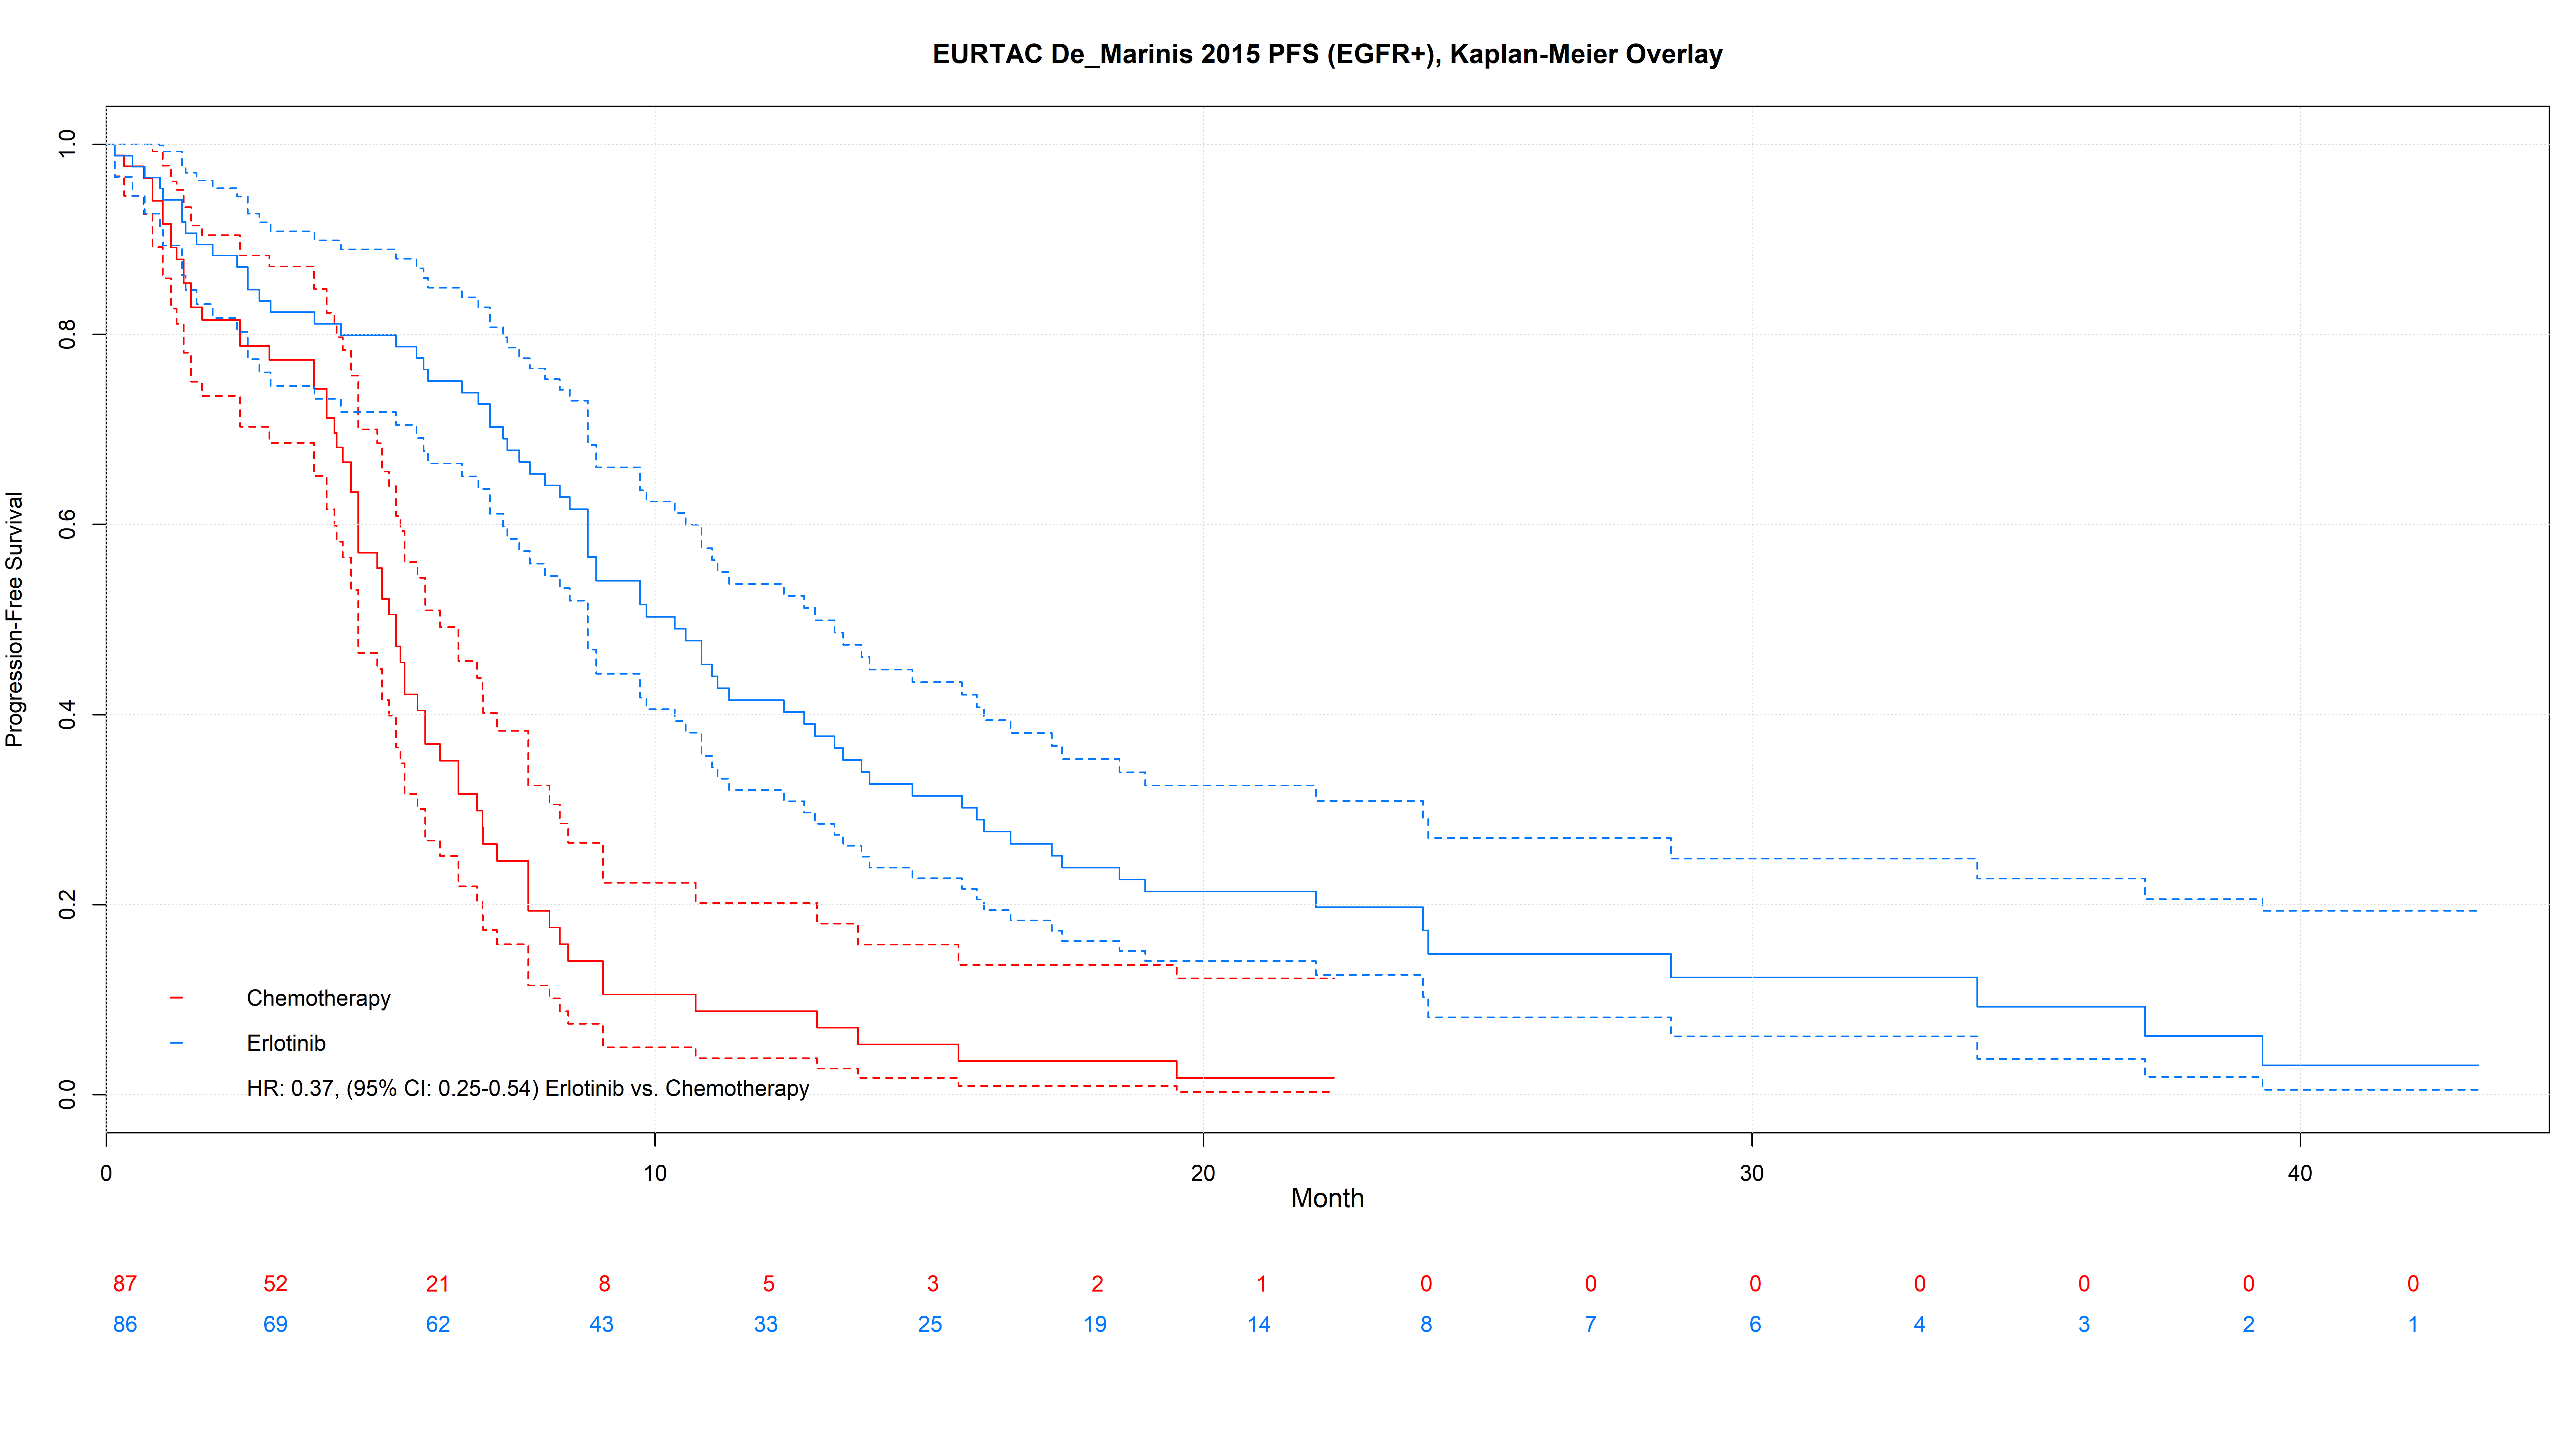
\includegraphics[max size={\textwidth}{\textheight}]{figs/km-plots/EURTAC De_Marinis 2015 PFS (EGFR+) Kaplan Meier.png}
\end{subfigure}
\begin{subfigure}{\textwidth}
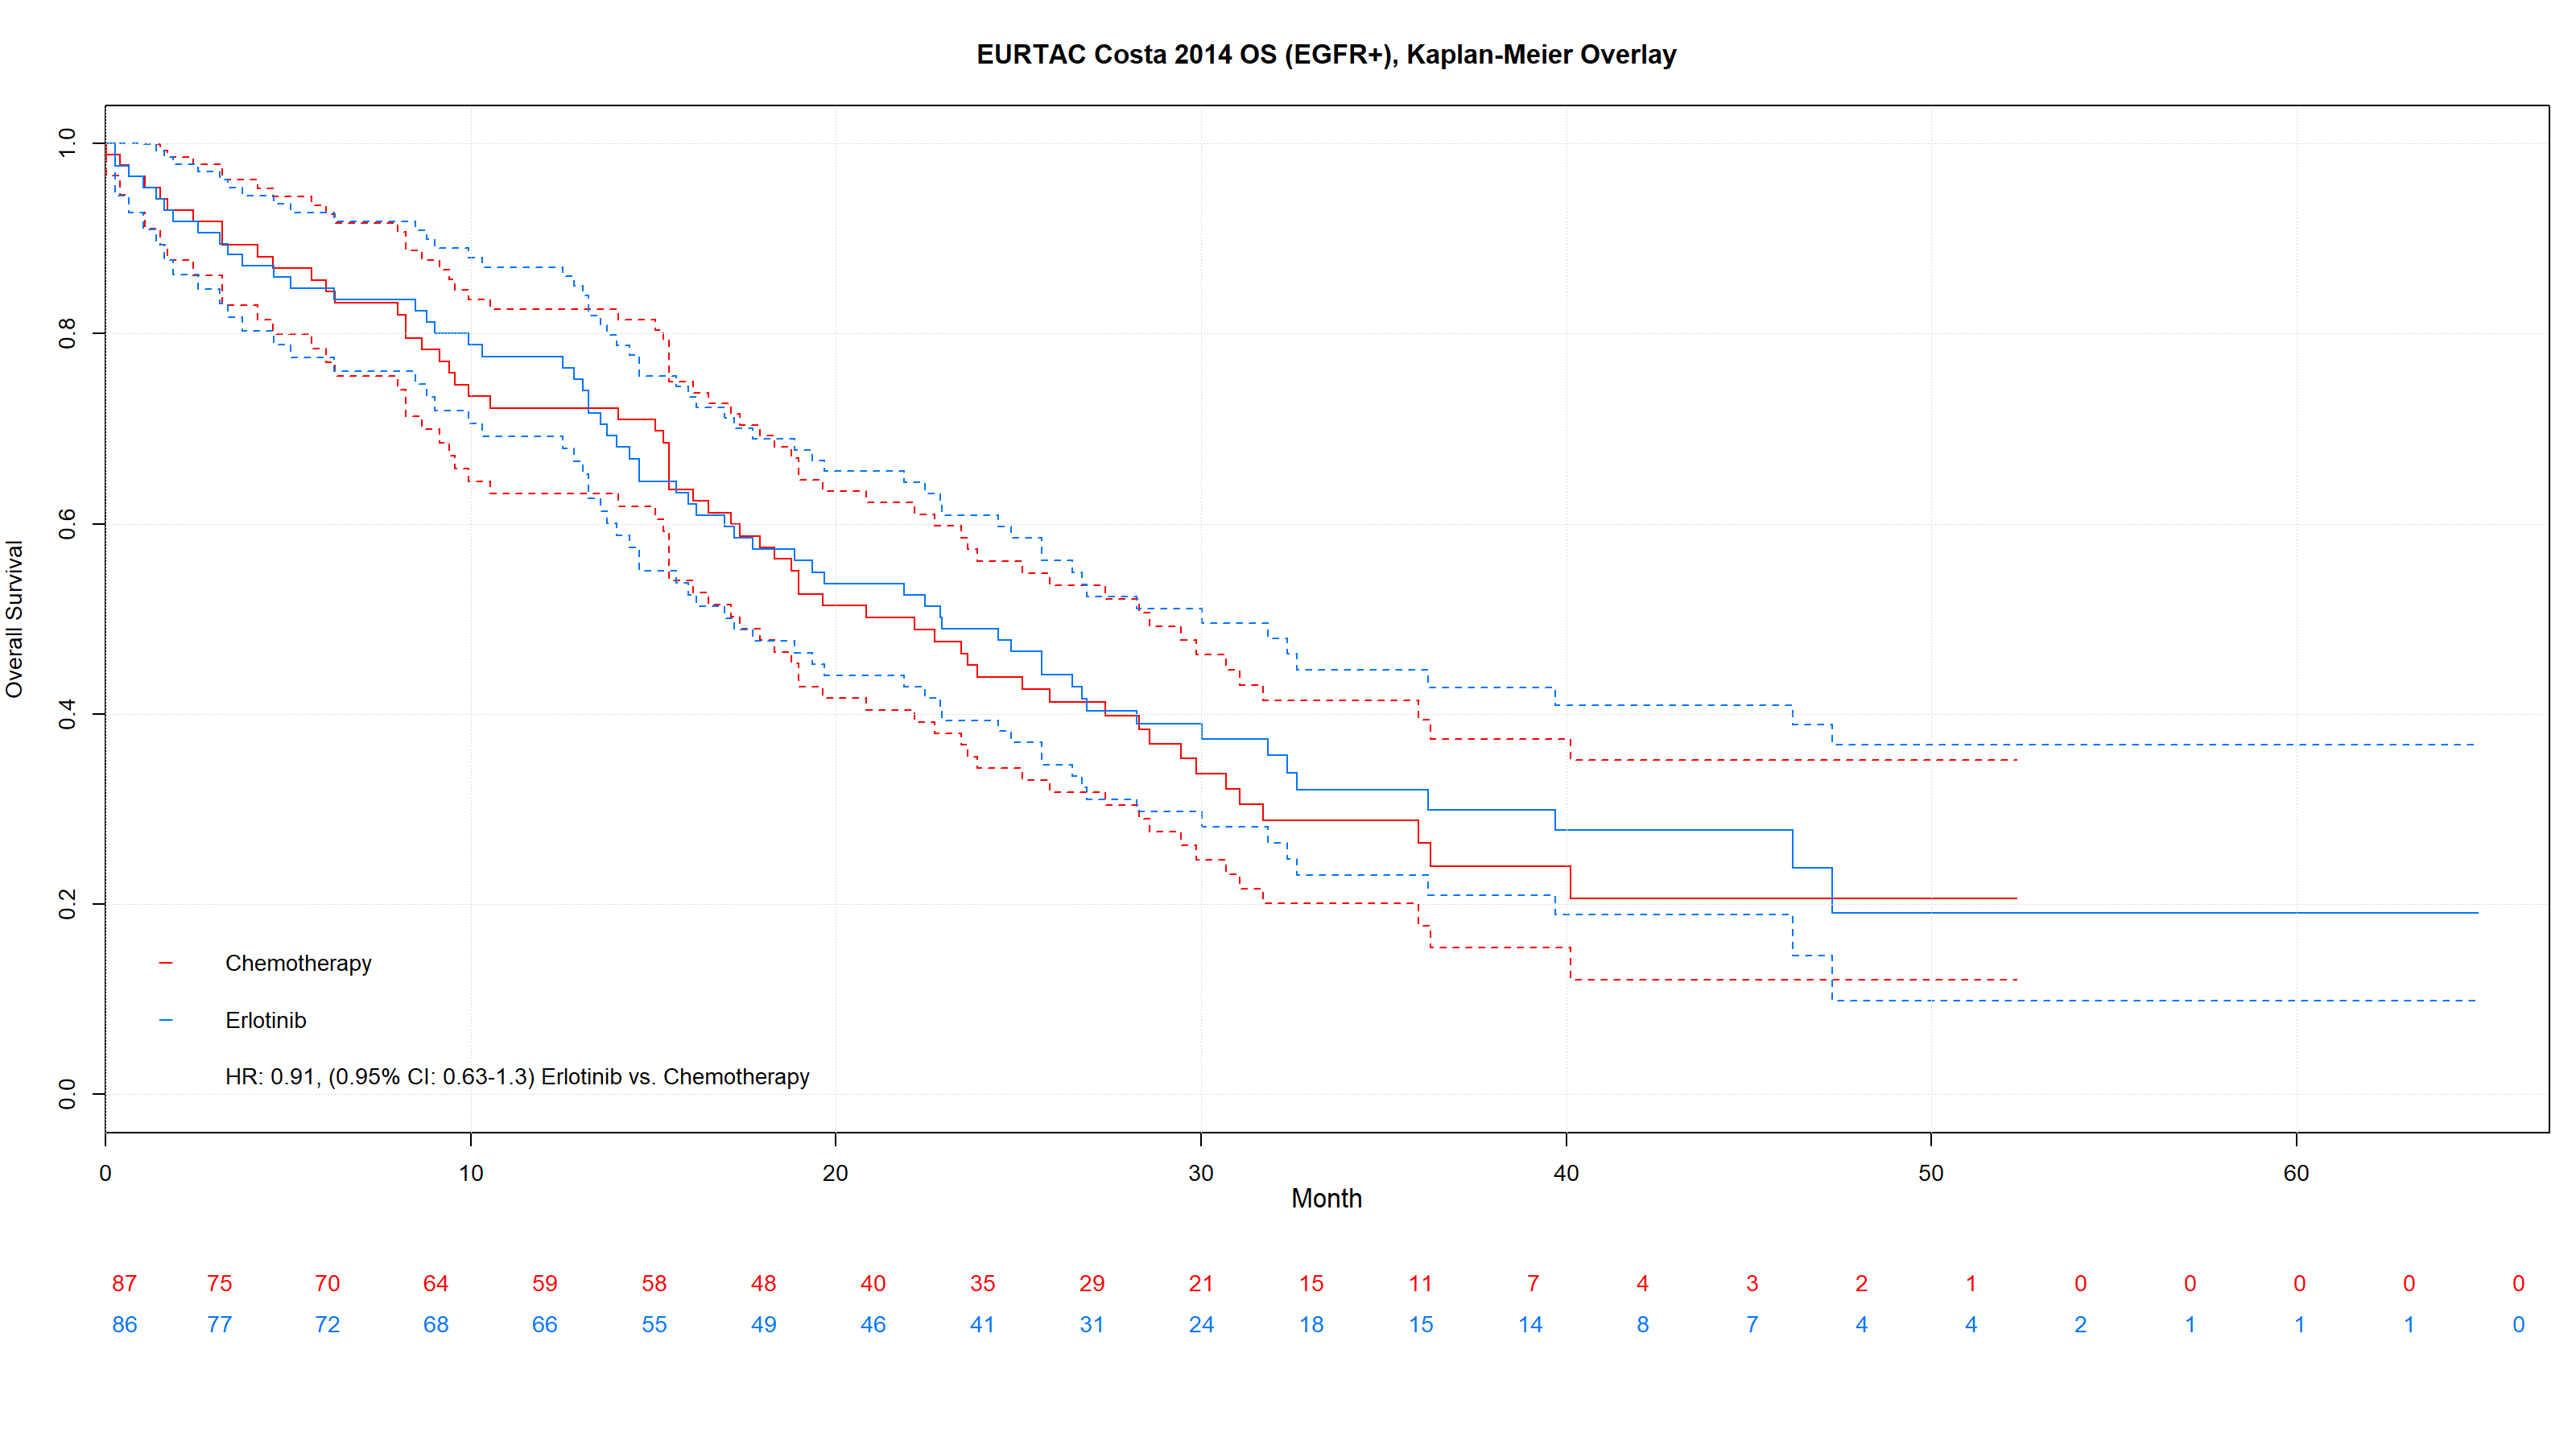
\includegraphics[max size={\textwidth}{\textheight}]{figs/km-plots/EURTAC Costa 2014 OS (EGFR+) Kaplan Meier.png}
\end{subfigure}
\centering
\caption{EURTAC, progression-free survival and overall survival}\label{fig:EURTAC}
\end{figure}


\begin{figure}
\centering
\begin{subfigure}{\textwidth}
\centering
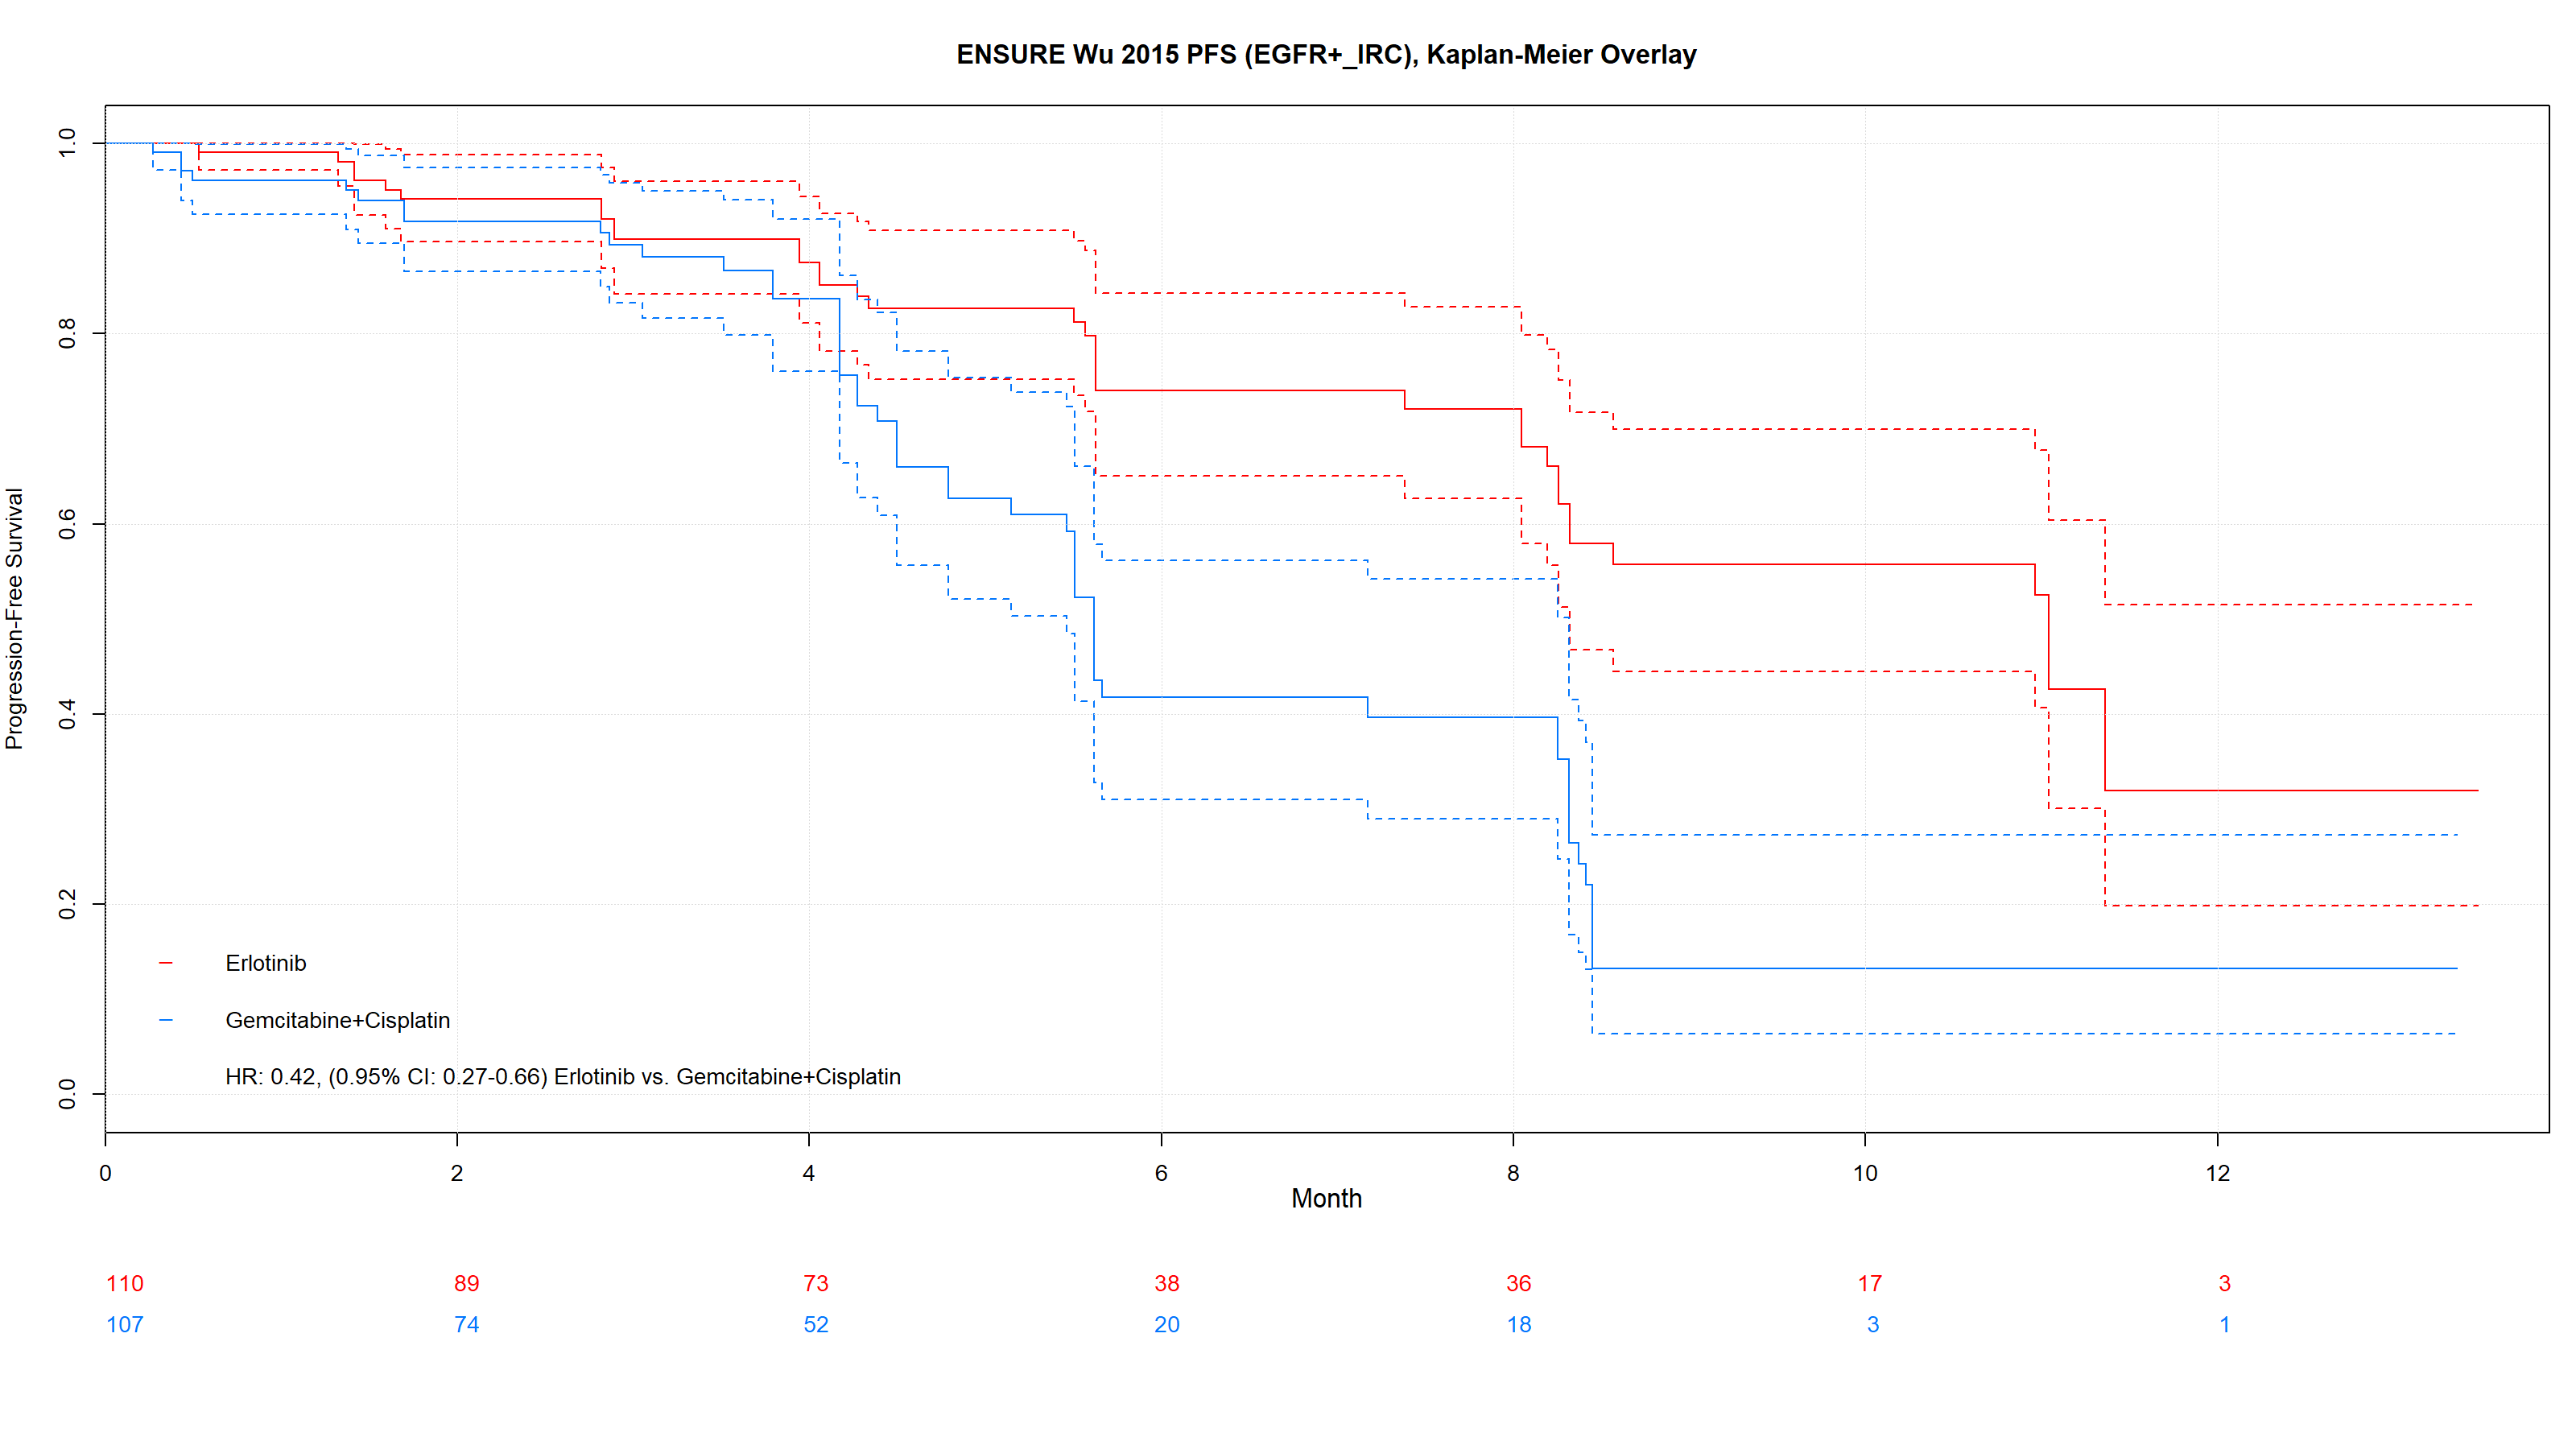
\includegraphics[max size={\textwidth}{\textheight}]{figs/km-plots/ENSURE Wu 2015 PFS (EGFR+_IRC) Kaplan Meier.png}
\end{subfigure}
\begin{subfigure}{\textwidth}
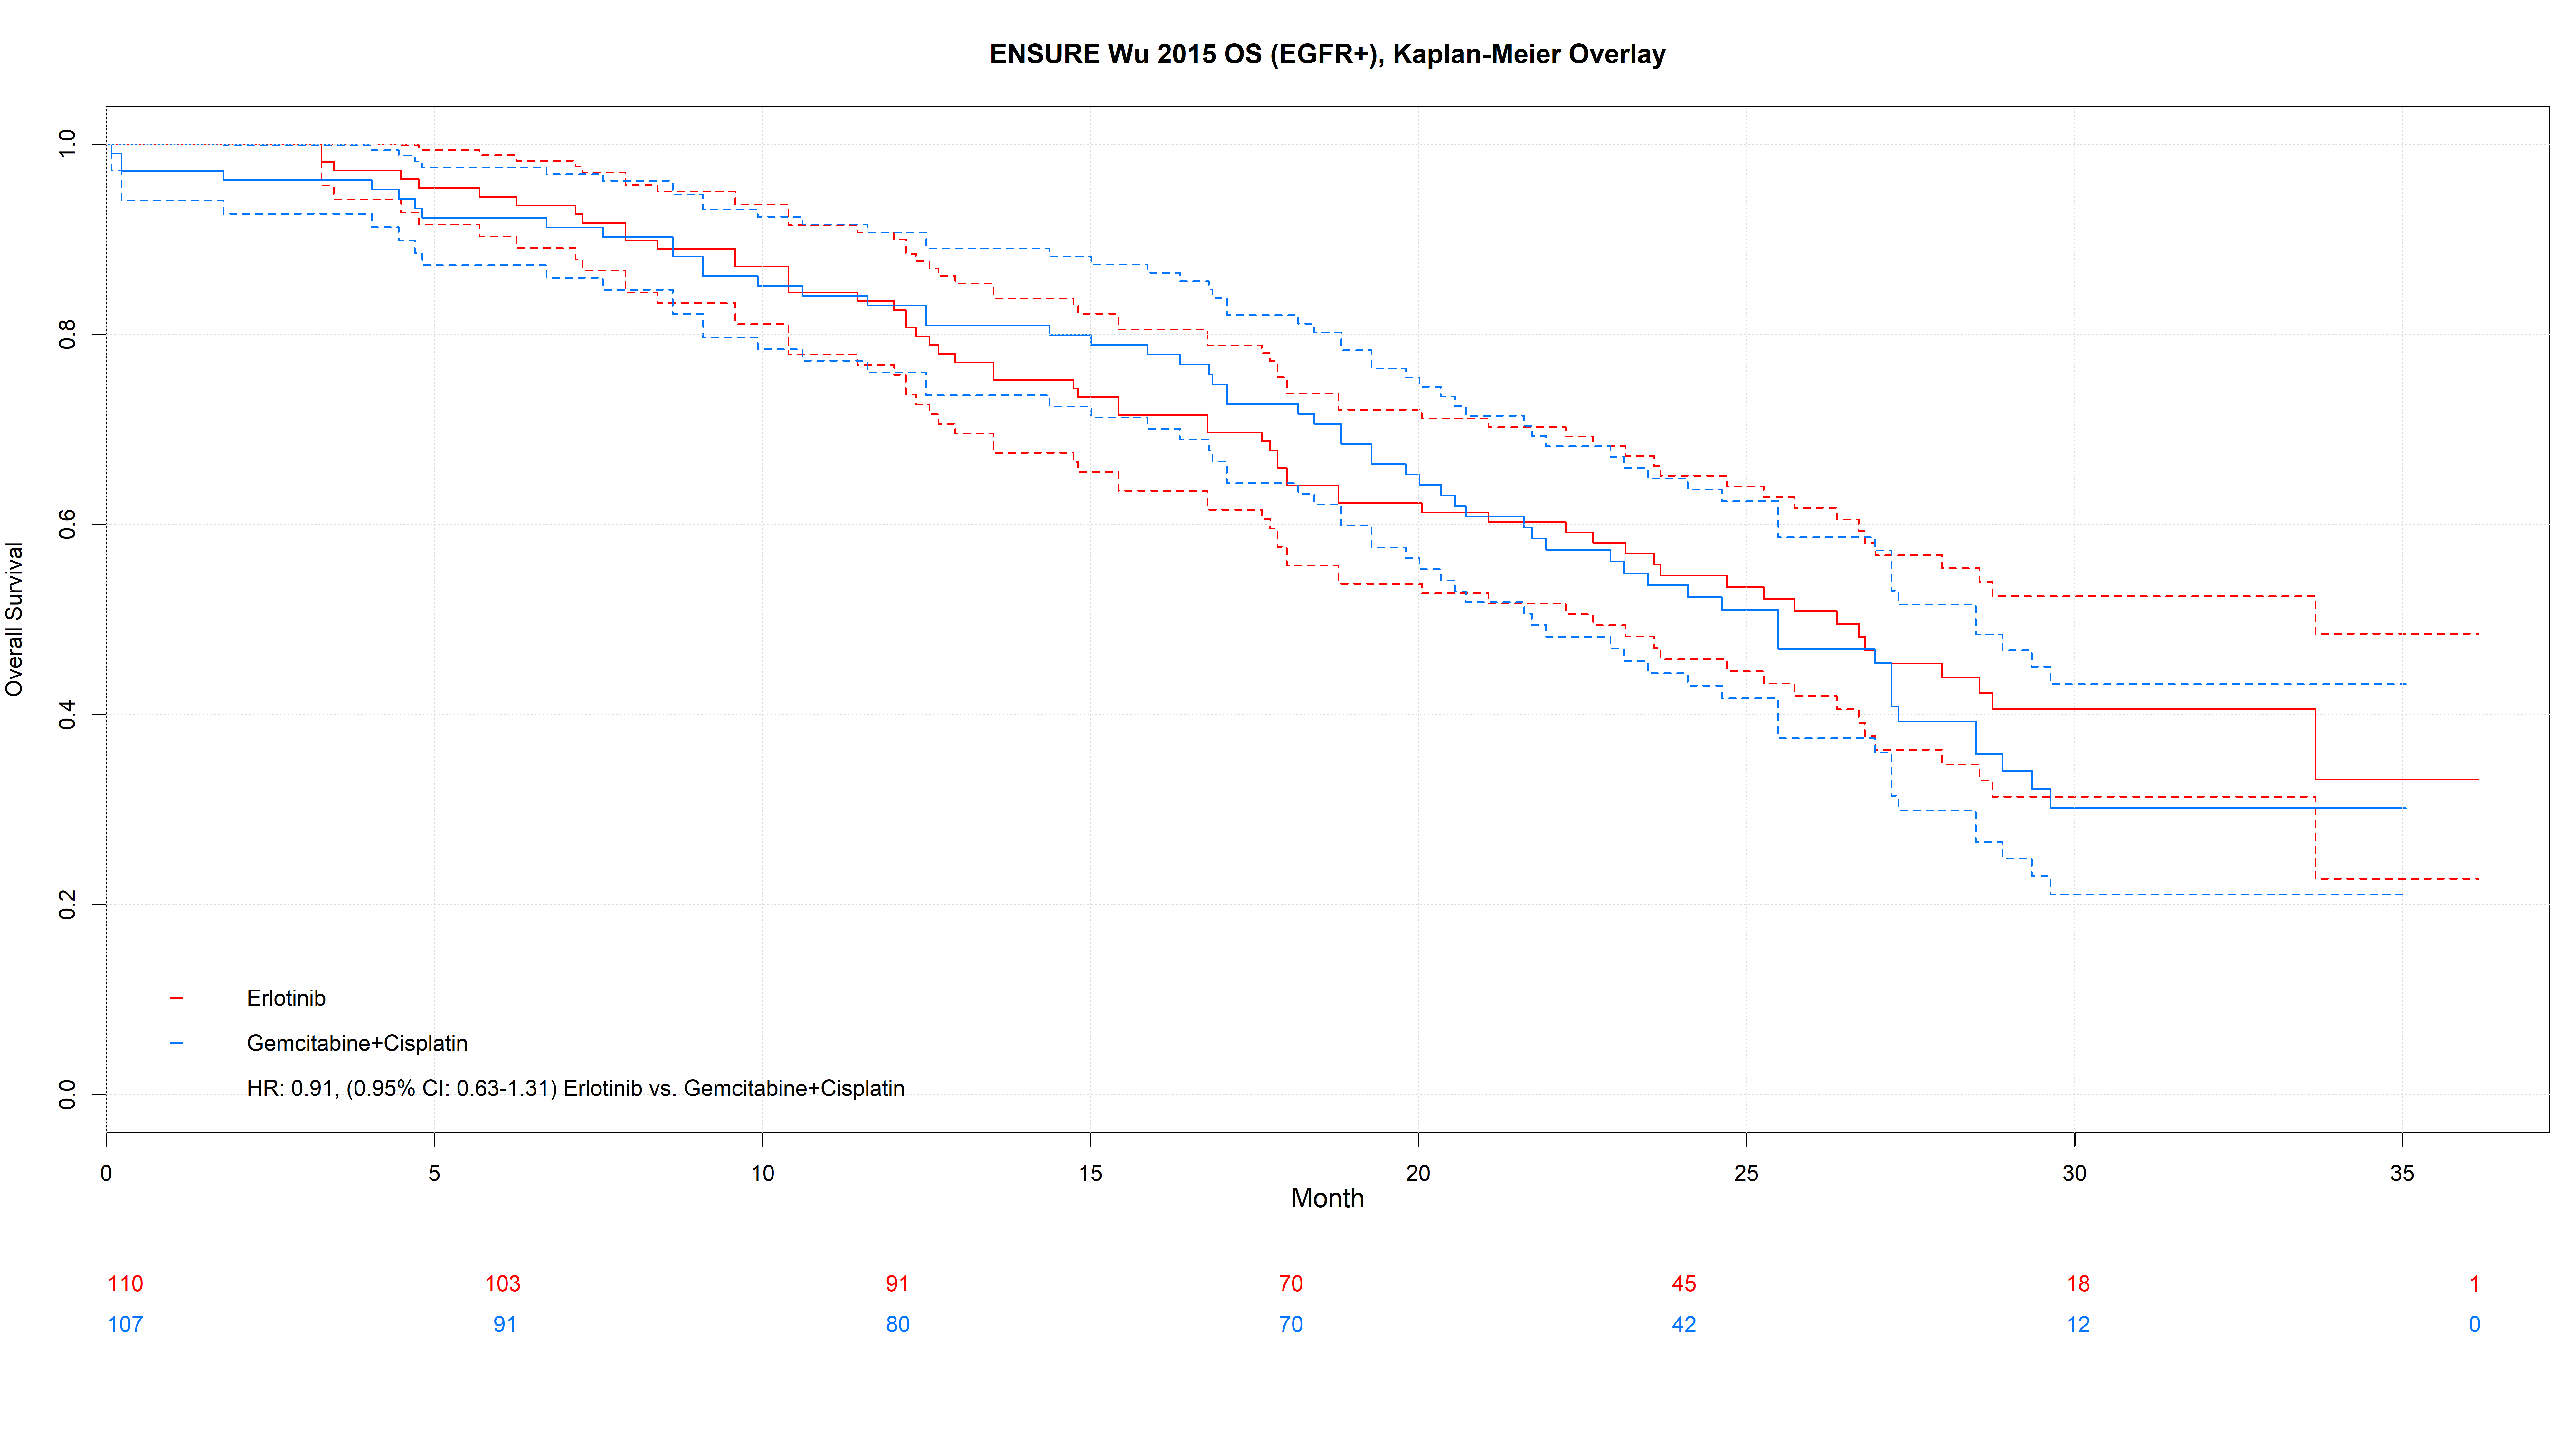
\includegraphics[max size={\textwidth}{\textheight}]{figs/km-plots/ENSURE Wu 2015 OS (EGFR+) Kaplan Meier.png}
\end{subfigure}
\centering
\caption{ENSURE, progression-free survival and overall survival}\label{fig:ENSURE}
\end{figure}



\begin{figure}
\centering
\begin{subfigure}{\textwidth}
\centering
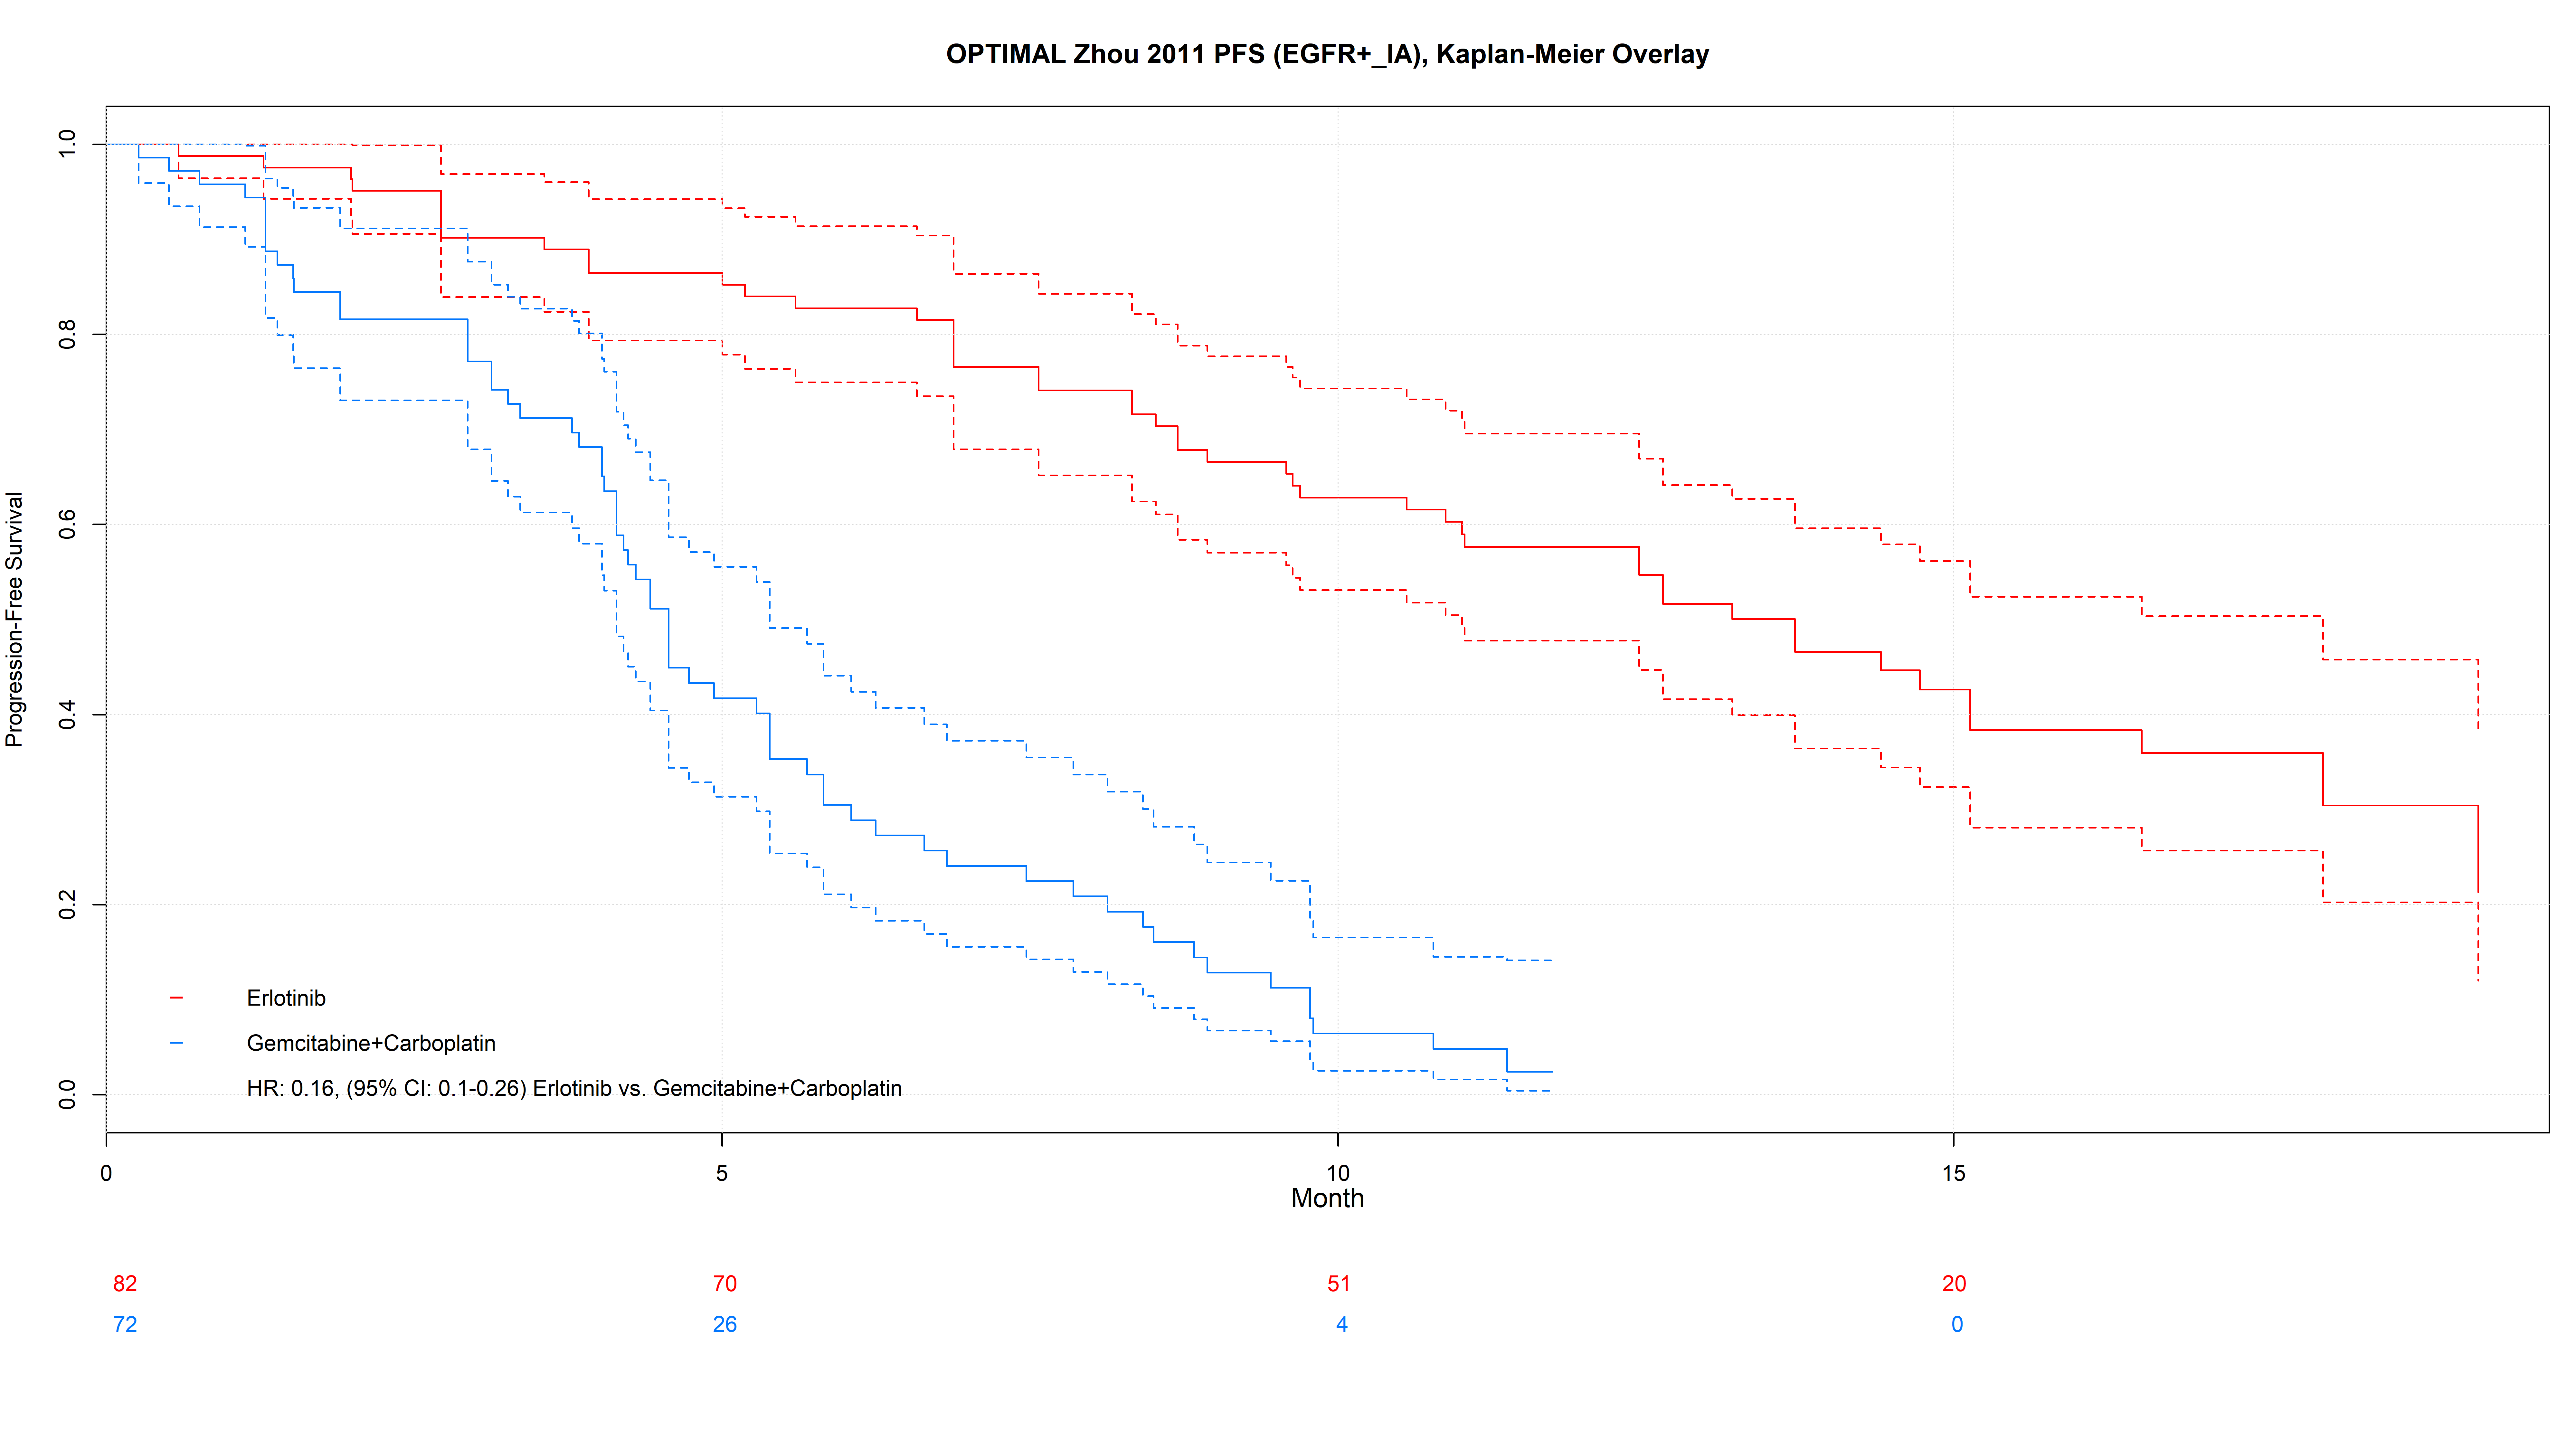
\includegraphics[max size={\textwidth}{\textheight}]{figs/km-plots/OPTIMAL Zhou 2011 PFS (EGFR+_IA) Kaplan Meier.png}
\end{subfigure}
\begin{subfigure}{\textwidth}
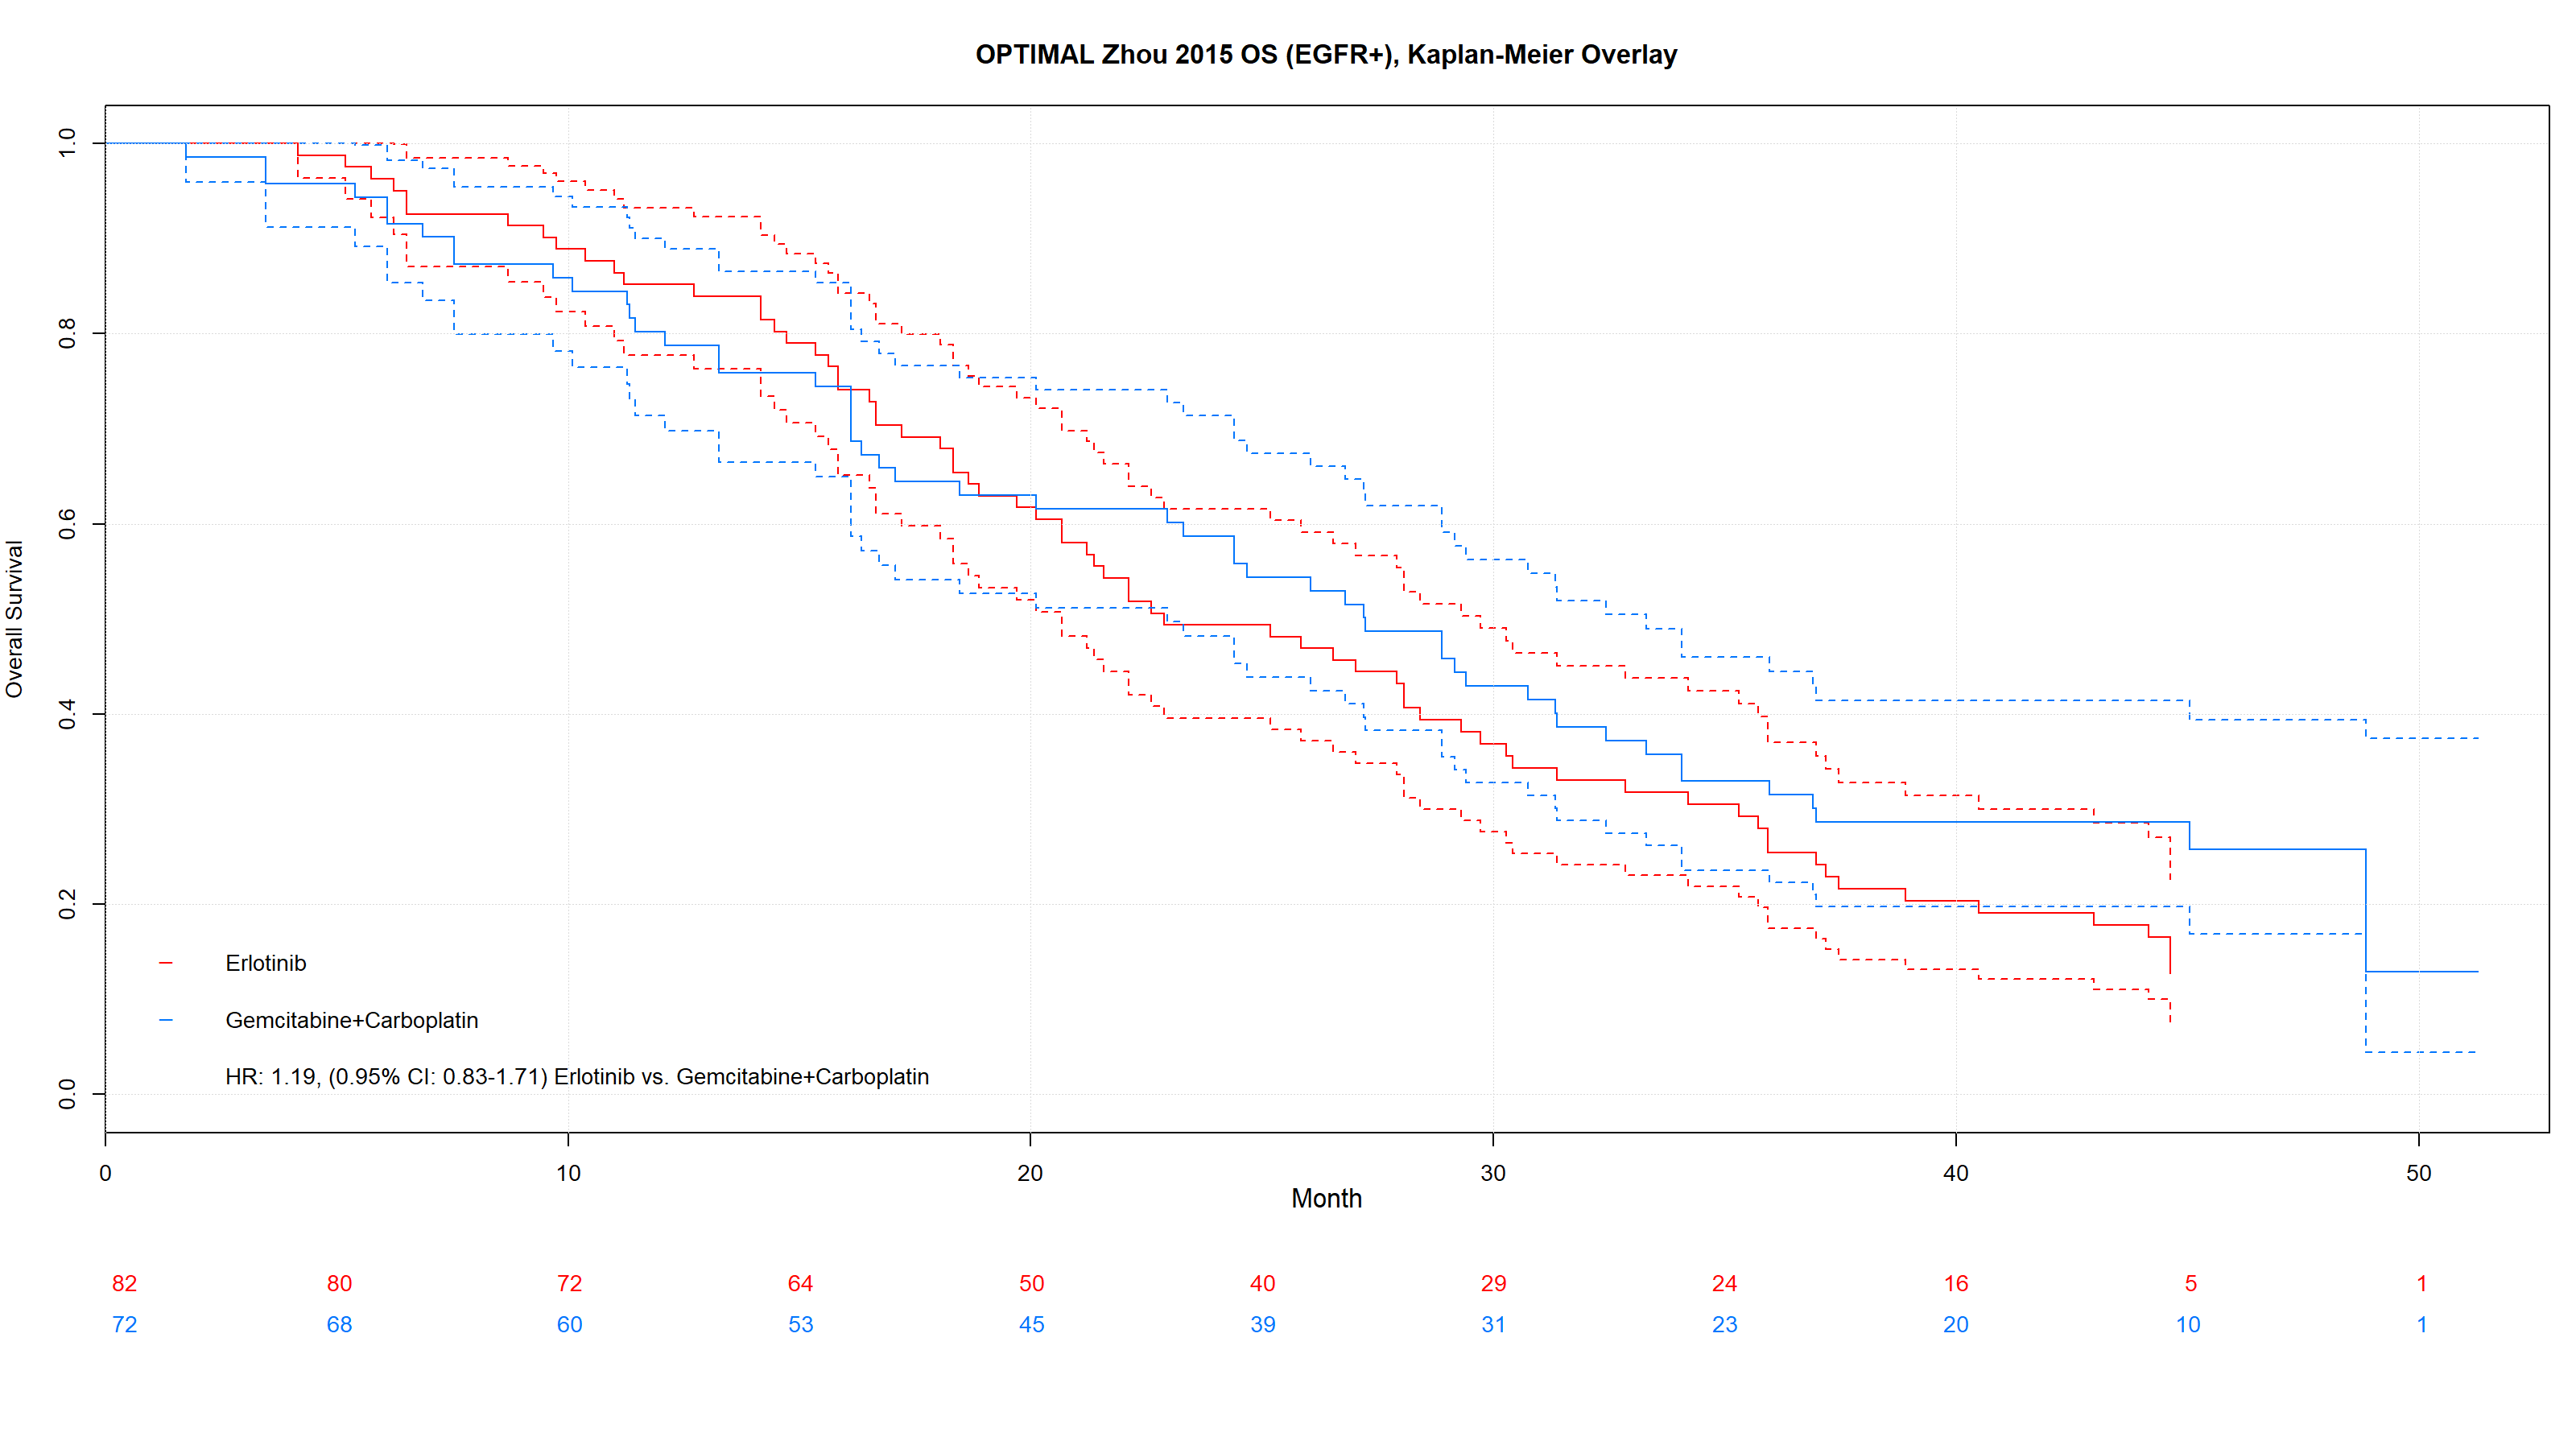
\includegraphics[max size={\textwidth}{\textheight}]{figs/km-plots/OPTIMAL Zhou 2015 OS (EGFR+) Kaplan Meier.png}
\end{subfigure}
\centering
\caption{OPTIMAL, progression-free survival and overall survival}\label{fig:OPTIMAL}
\end{figure}


\begin{figure}
\centering
\begin{subfigure}{\textwidth}
\centering
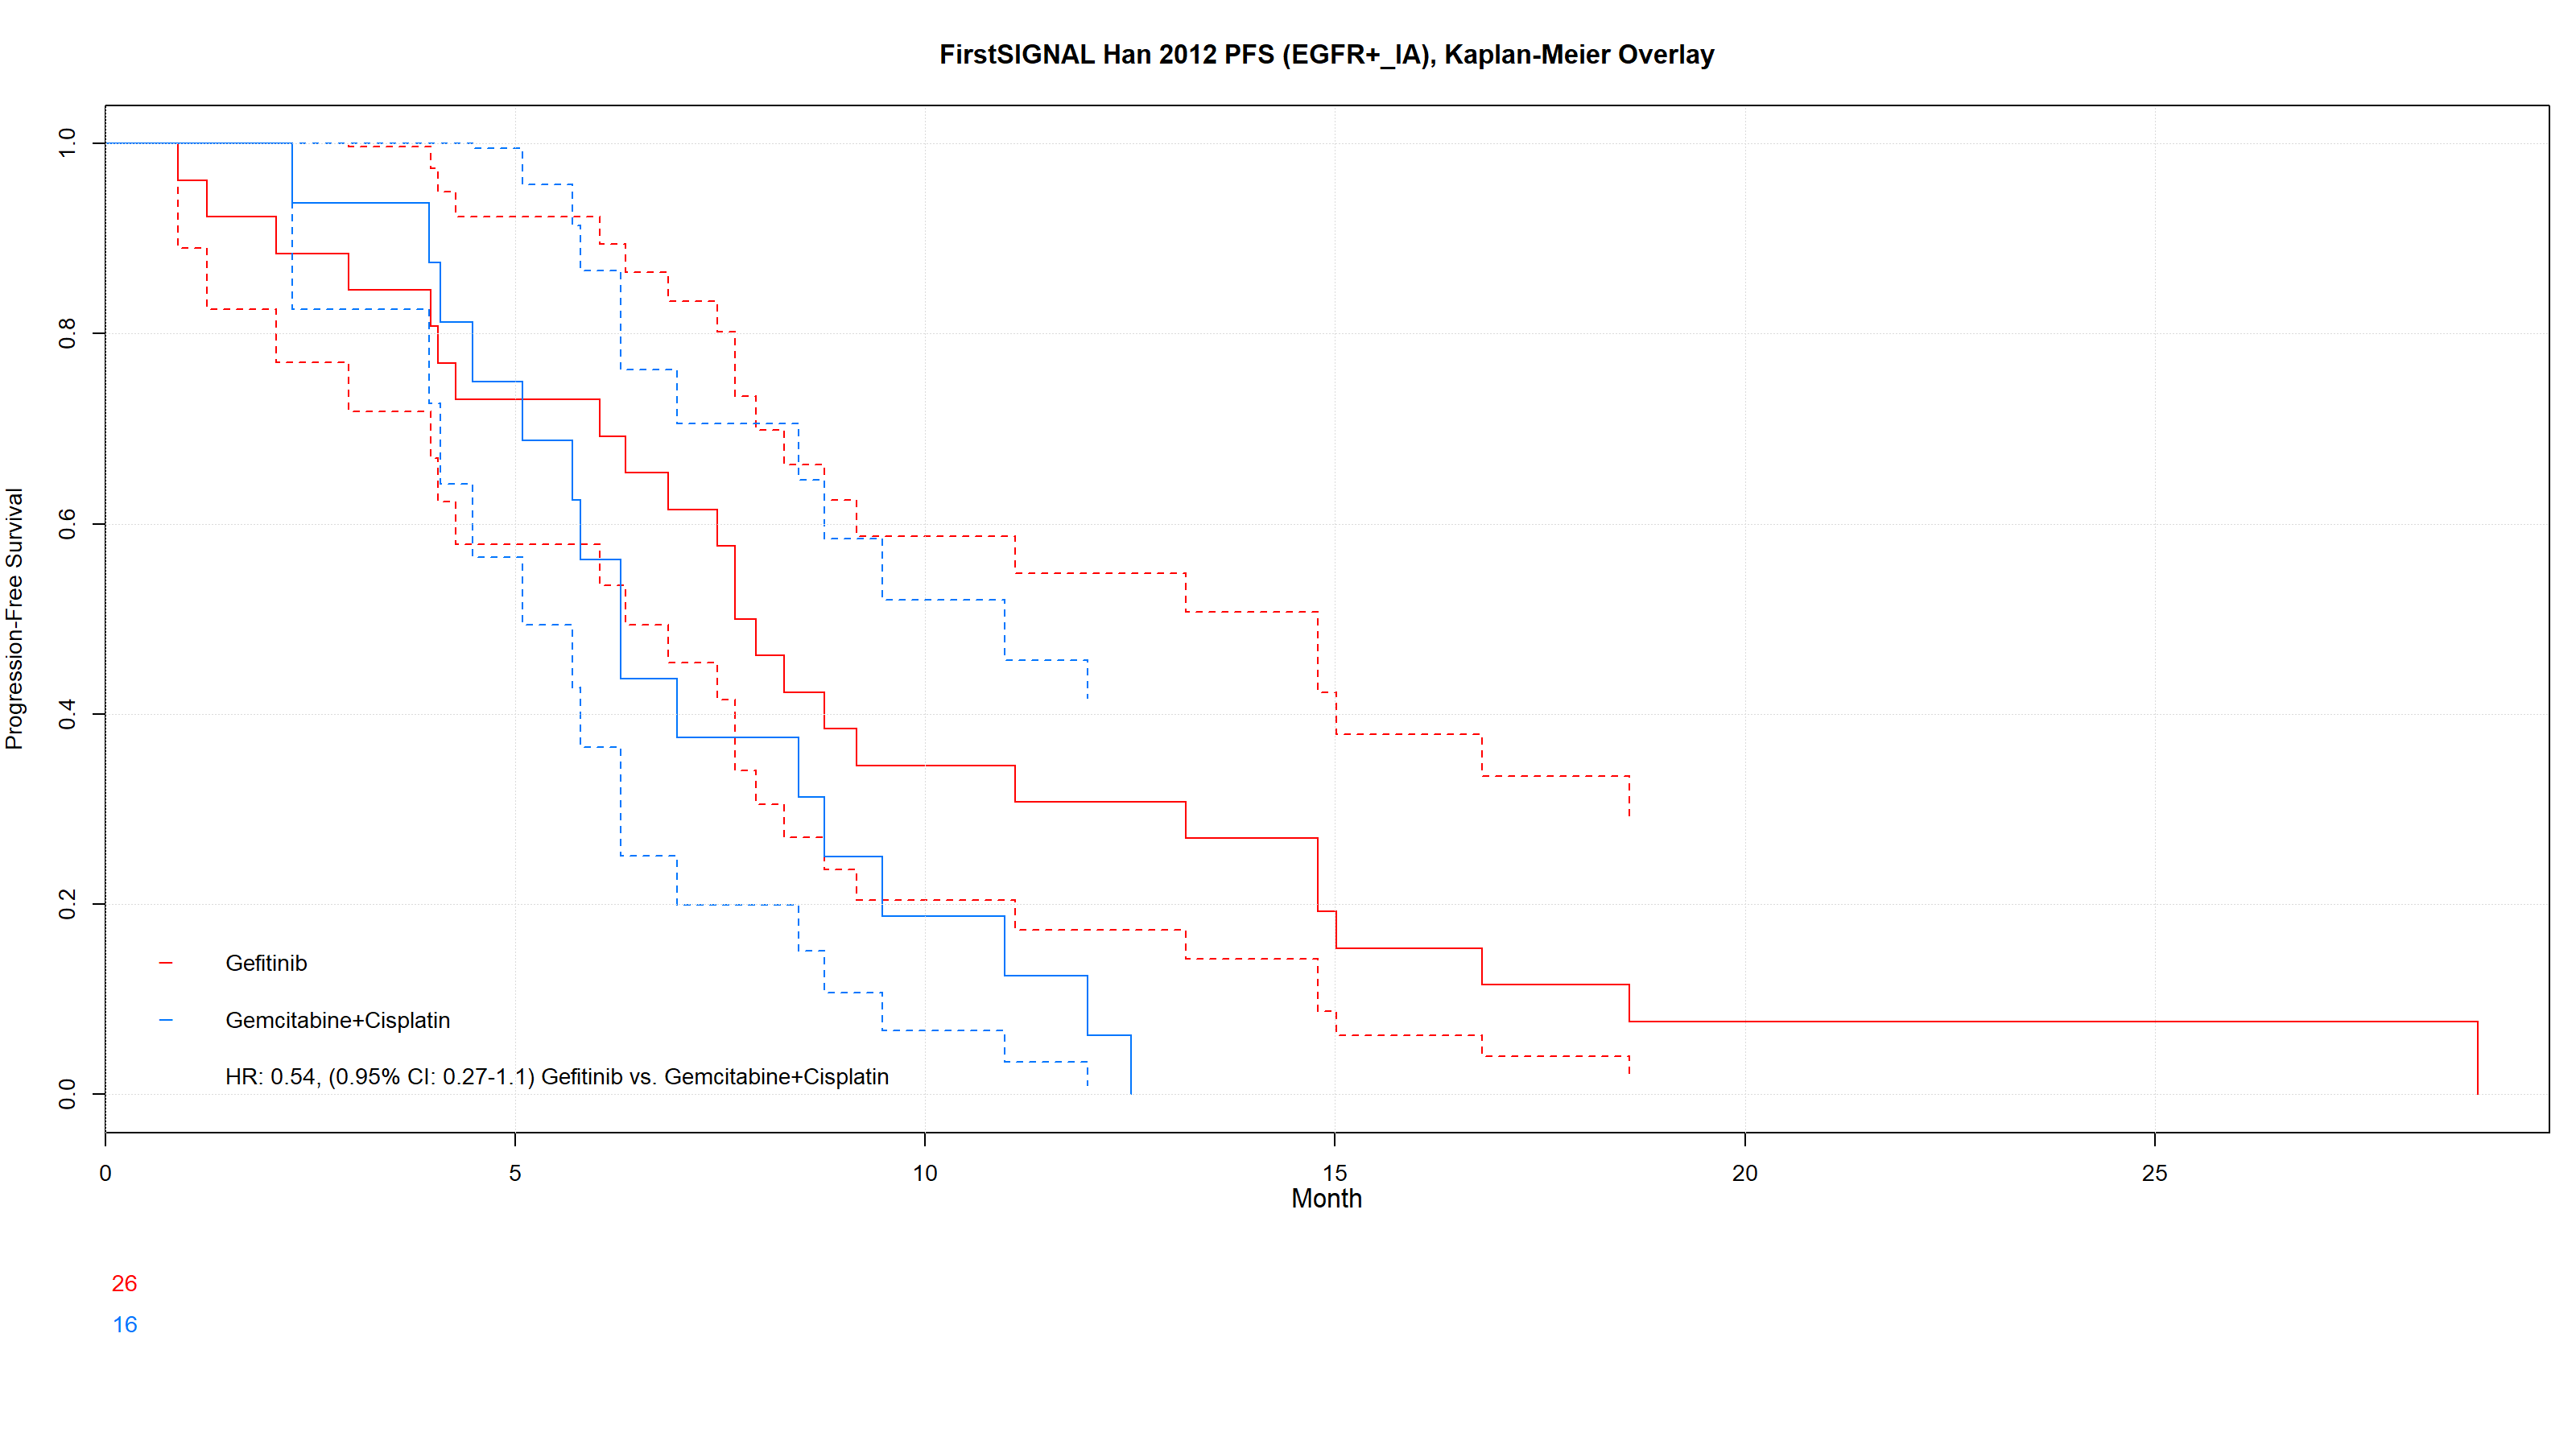
\includegraphics[max size={\textwidth}{\textheight}]{figs/km-plots/FirstSIGNAL Han 2012 PFS (EGFR+_IA) Kaplan Meier.png}
\end{subfigure}
\begin{subfigure}{\textwidth}
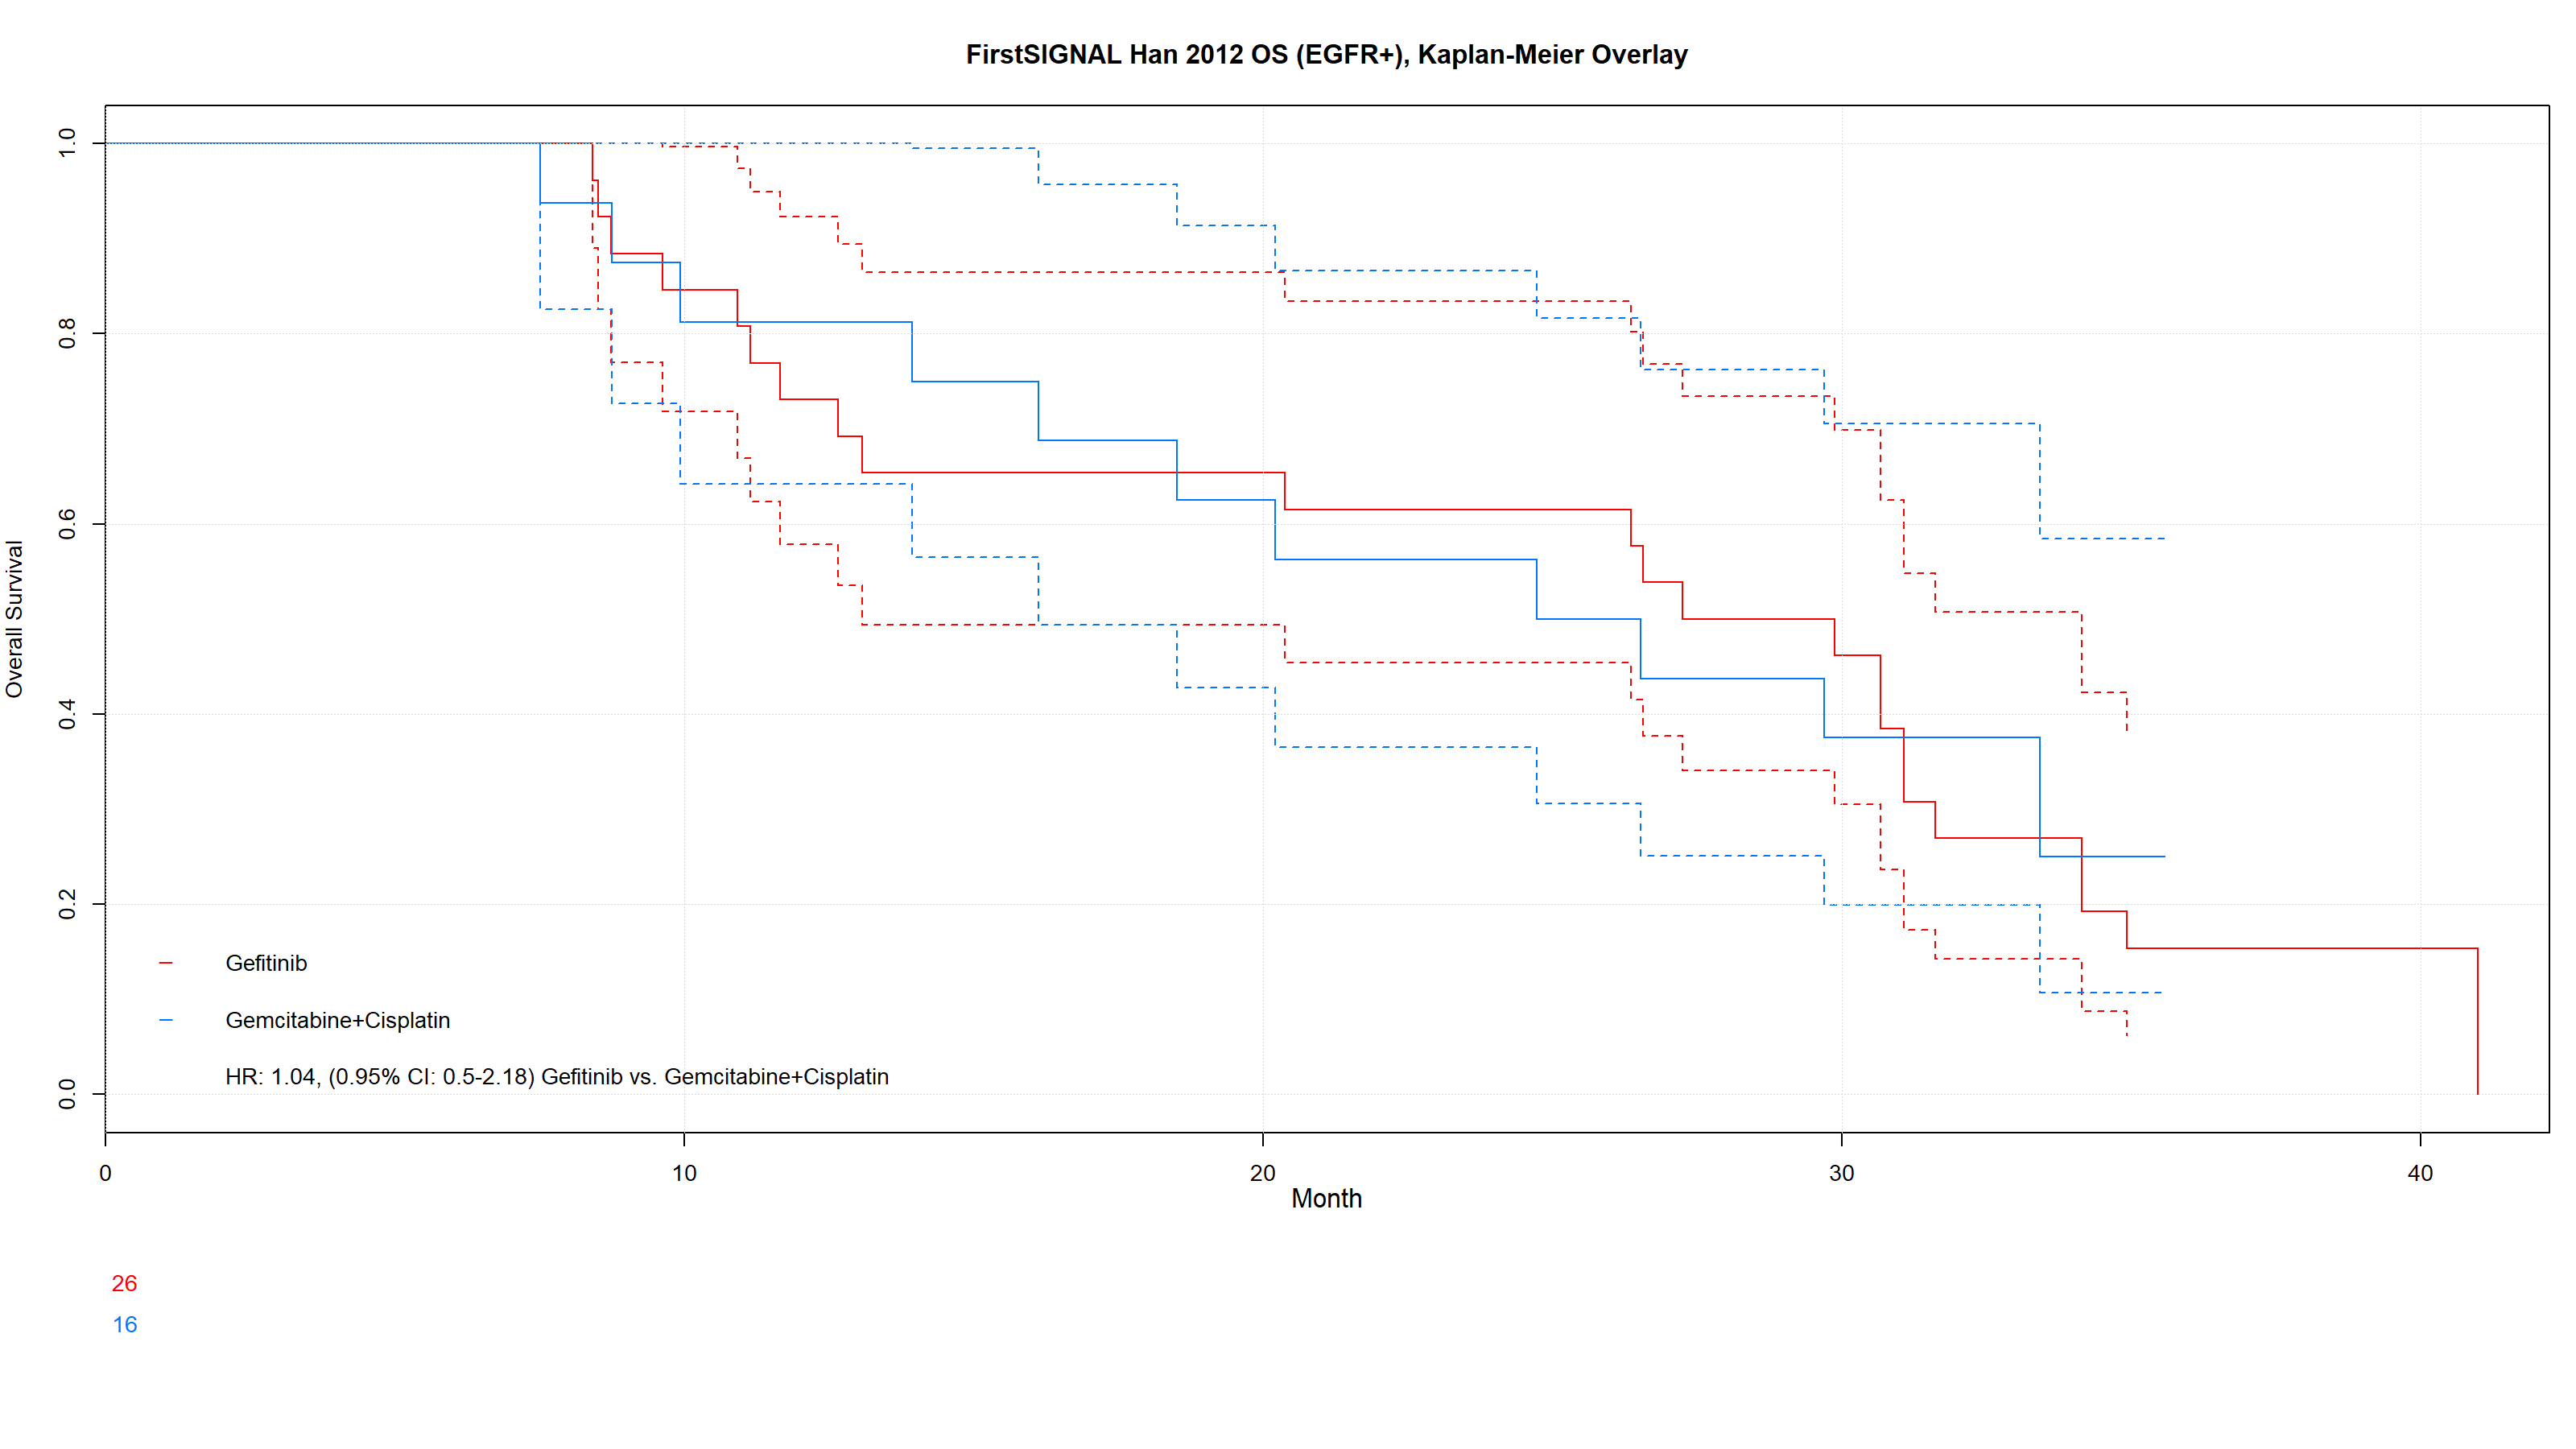
\includegraphics[max size={\textwidth}{\textheight}]{figs/km-plots/FirstSIGNAL Han 2012 OS (EGFR+) Kaplan Meier.png}
\end{subfigure}
\centering
\caption{FirstSIGNAL, progression-free survival and overall survival}\label{fig:firstSIGNAL}
\end{figure}


\begin{figure}
\centering
\begin{subfigure}{\textwidth}
\centering
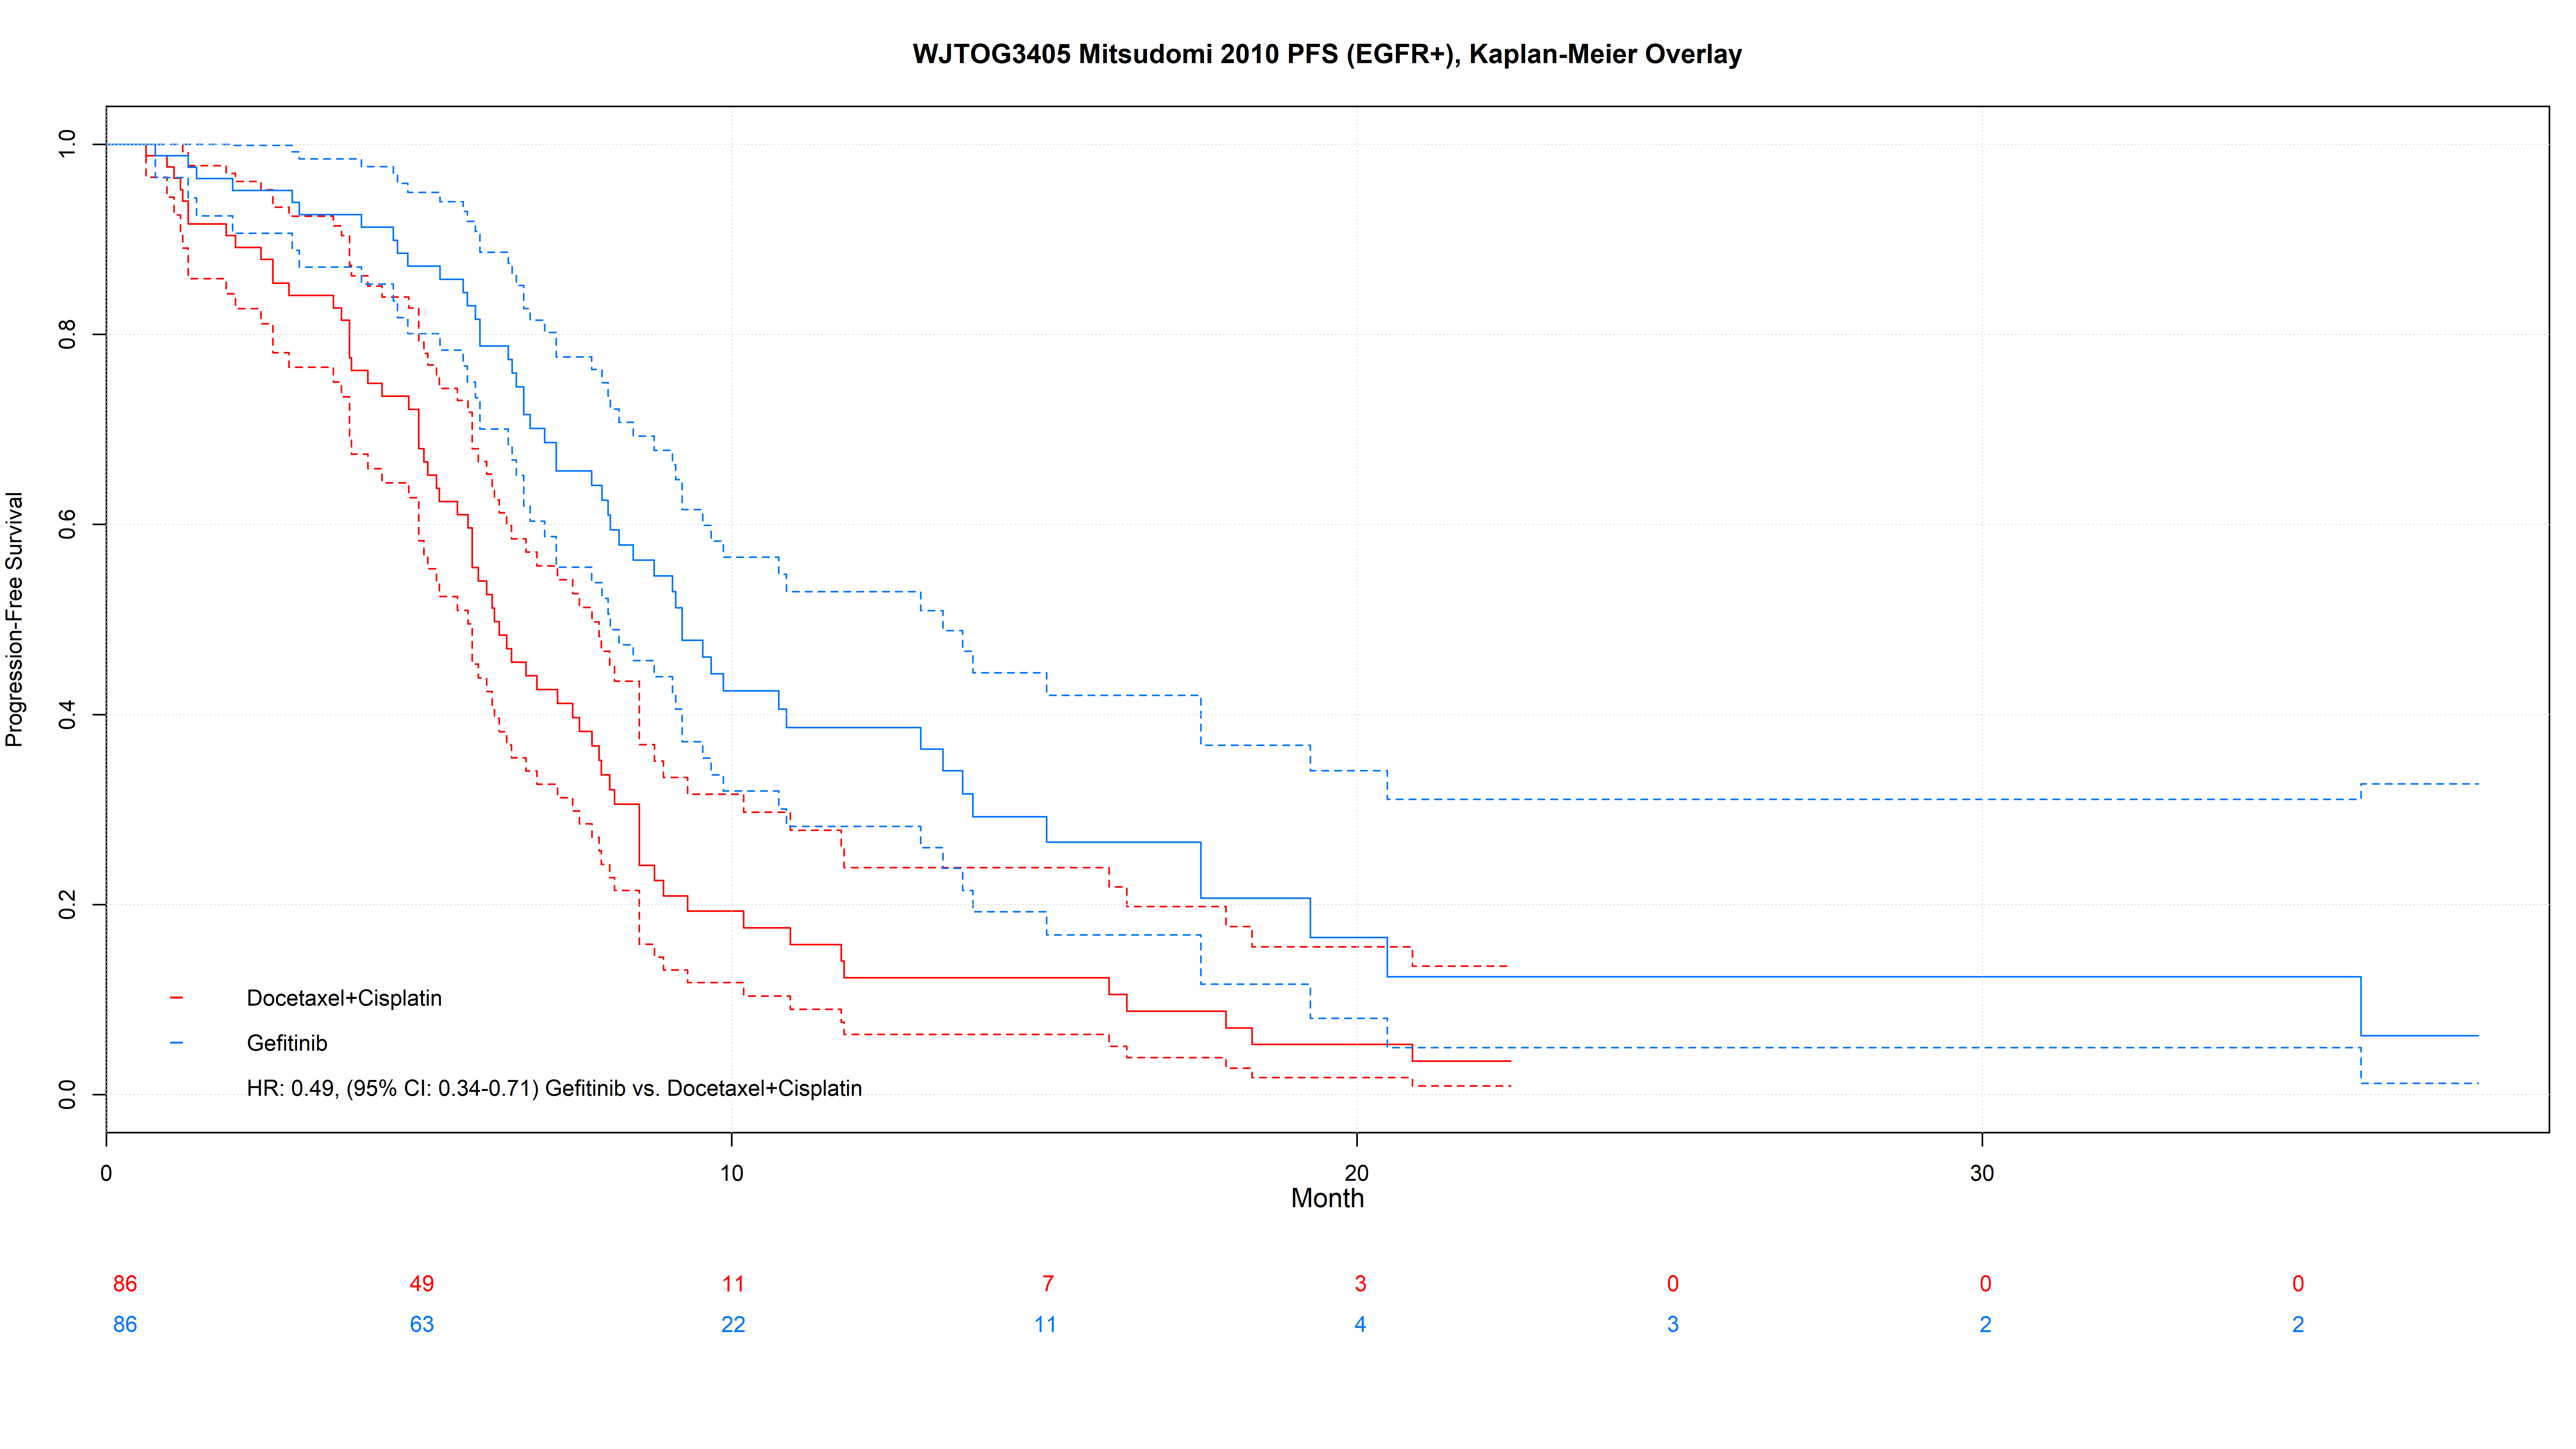
\includegraphics[max size={\textwidth}{\textheight}]{figs/km-plots/WJTOG3405 Mitsudomi 2010 PFS (EGFR+) Kaplan Meier.png}
\end{subfigure}
\begin{subfigure}{\textwidth}
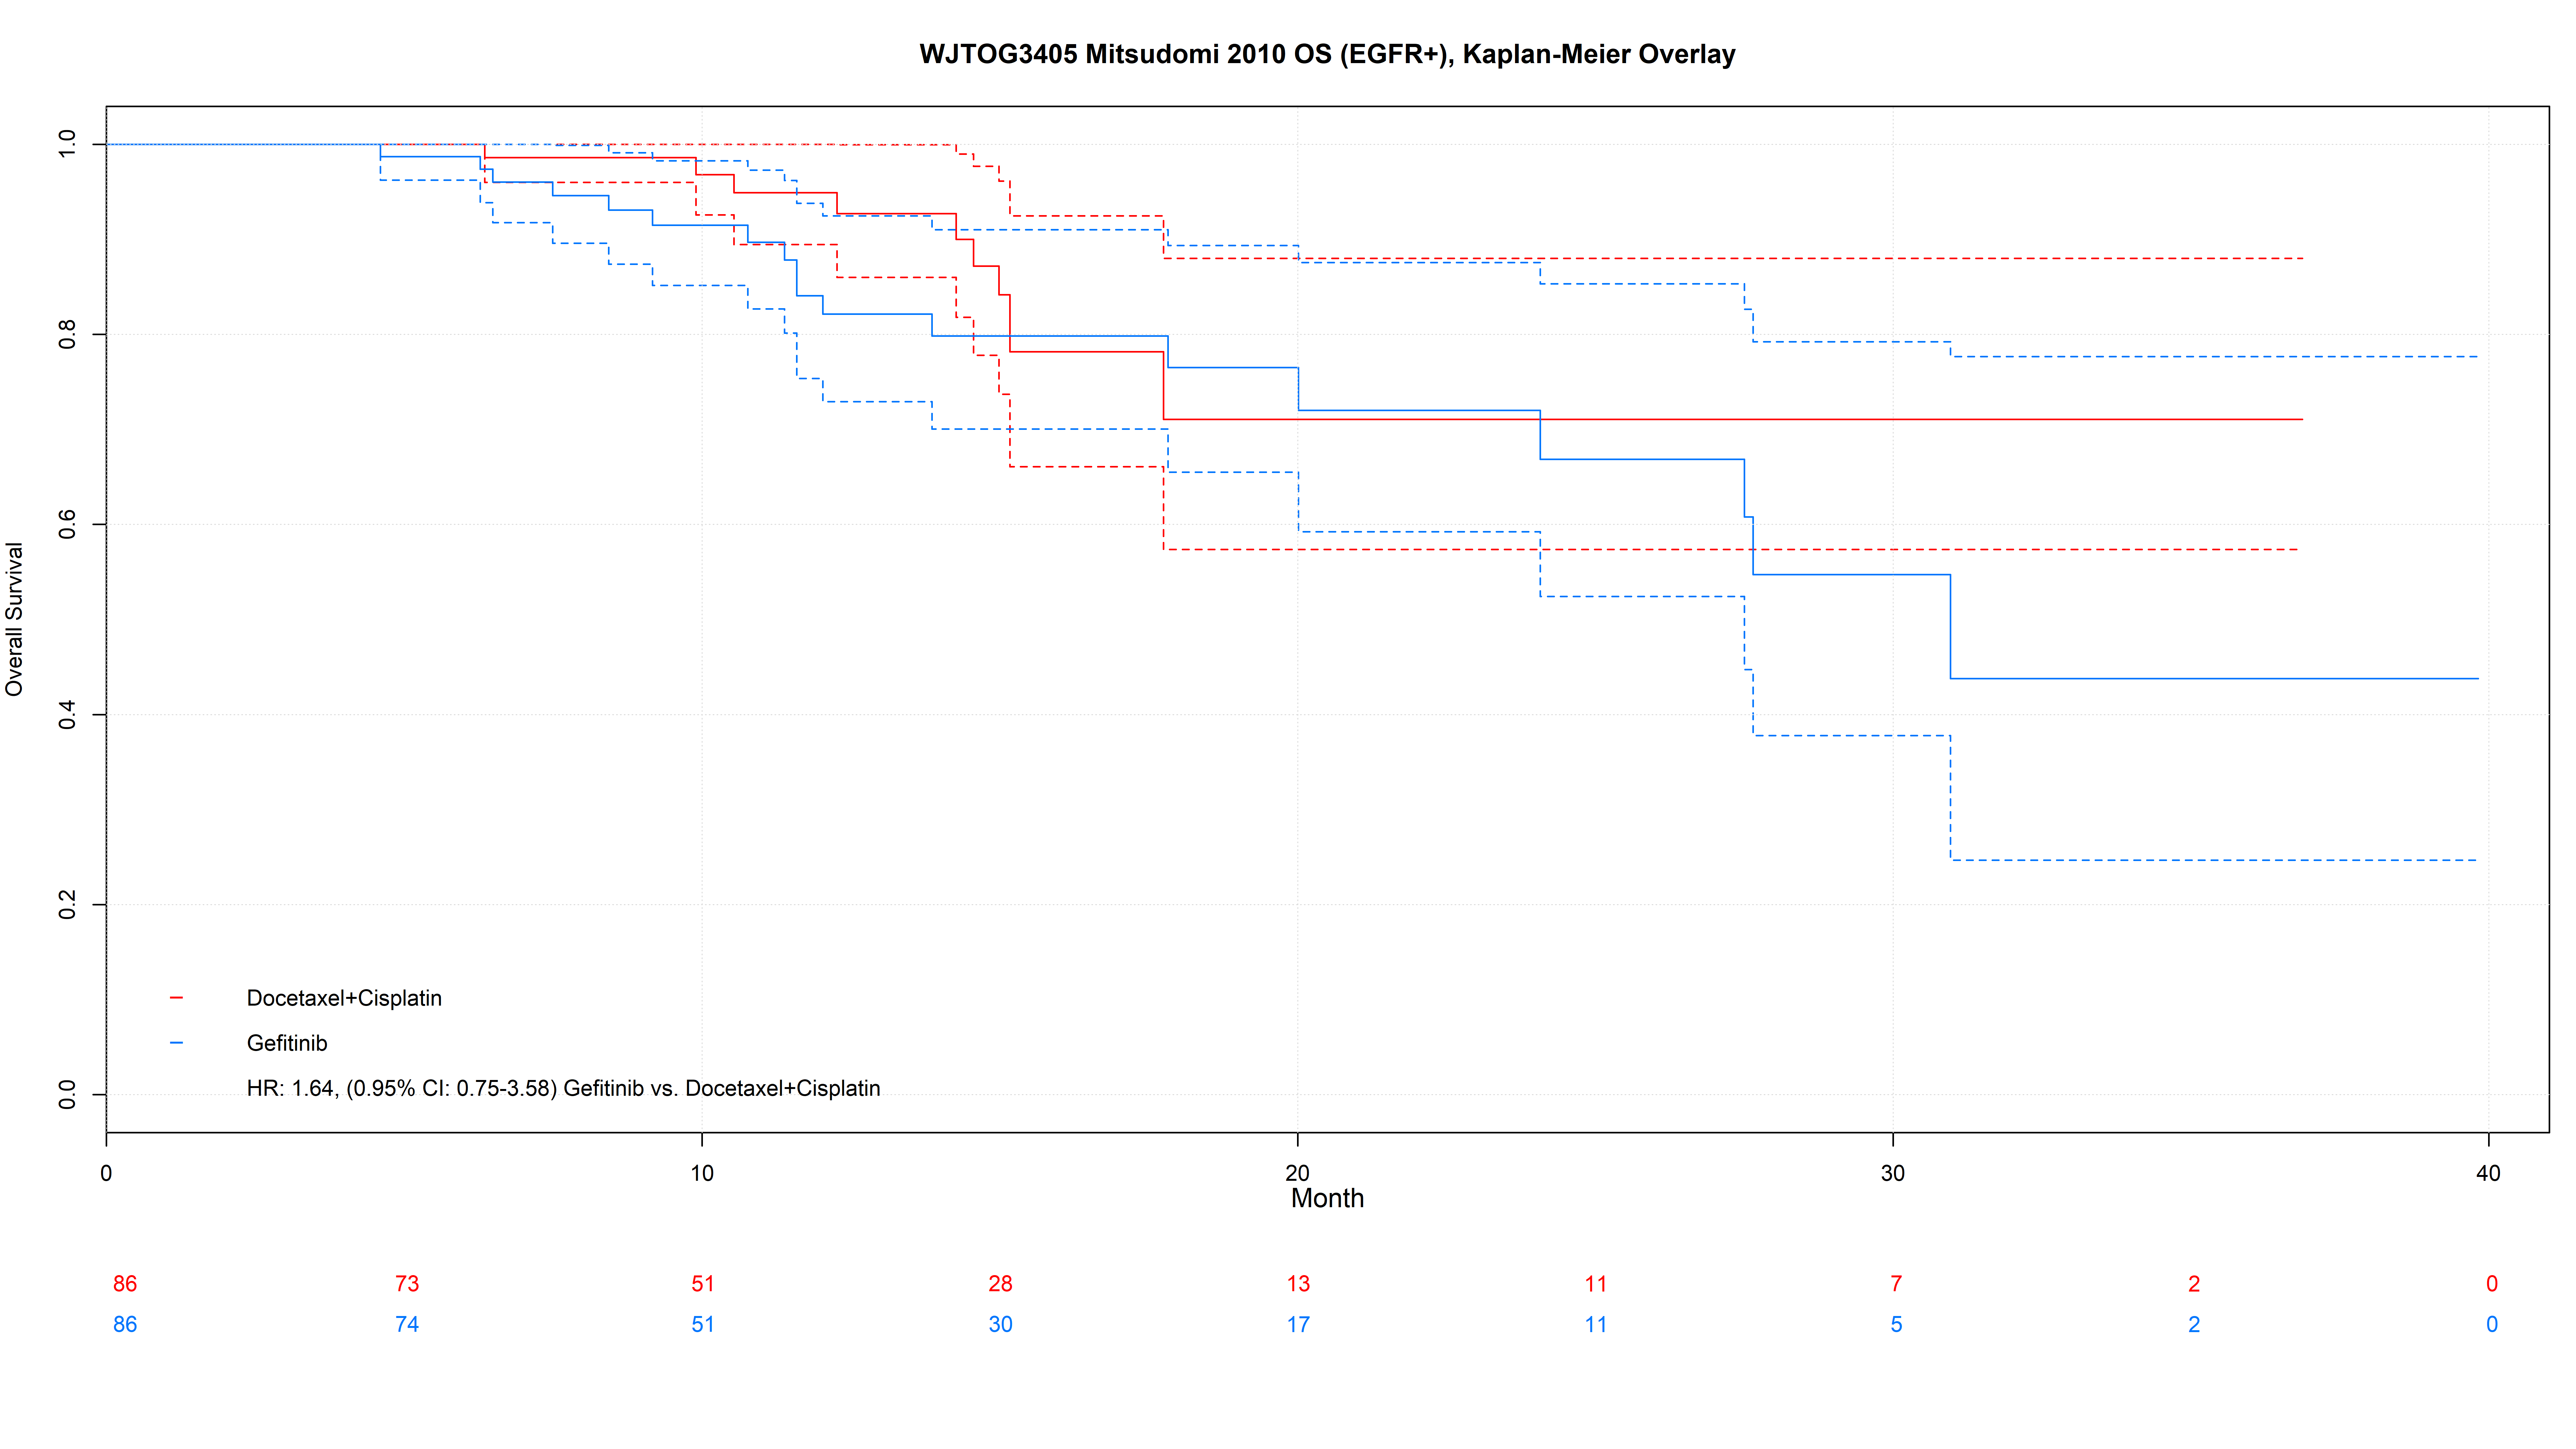
\includegraphics[max size={\textwidth}{\textheight}]{figs/km-plots/WJTOG3405 Mitsudomi 2010 OS (EGFR+) Kaplan Meier.png}
\end{subfigure}
\centering
\caption{WJTOG3405, progression-free survival and overall survival}\label{fig:WJTOG3405}
\end{figure}



\begin{figure}
\centering
\begin{subfigure}{\textwidth}
\centering
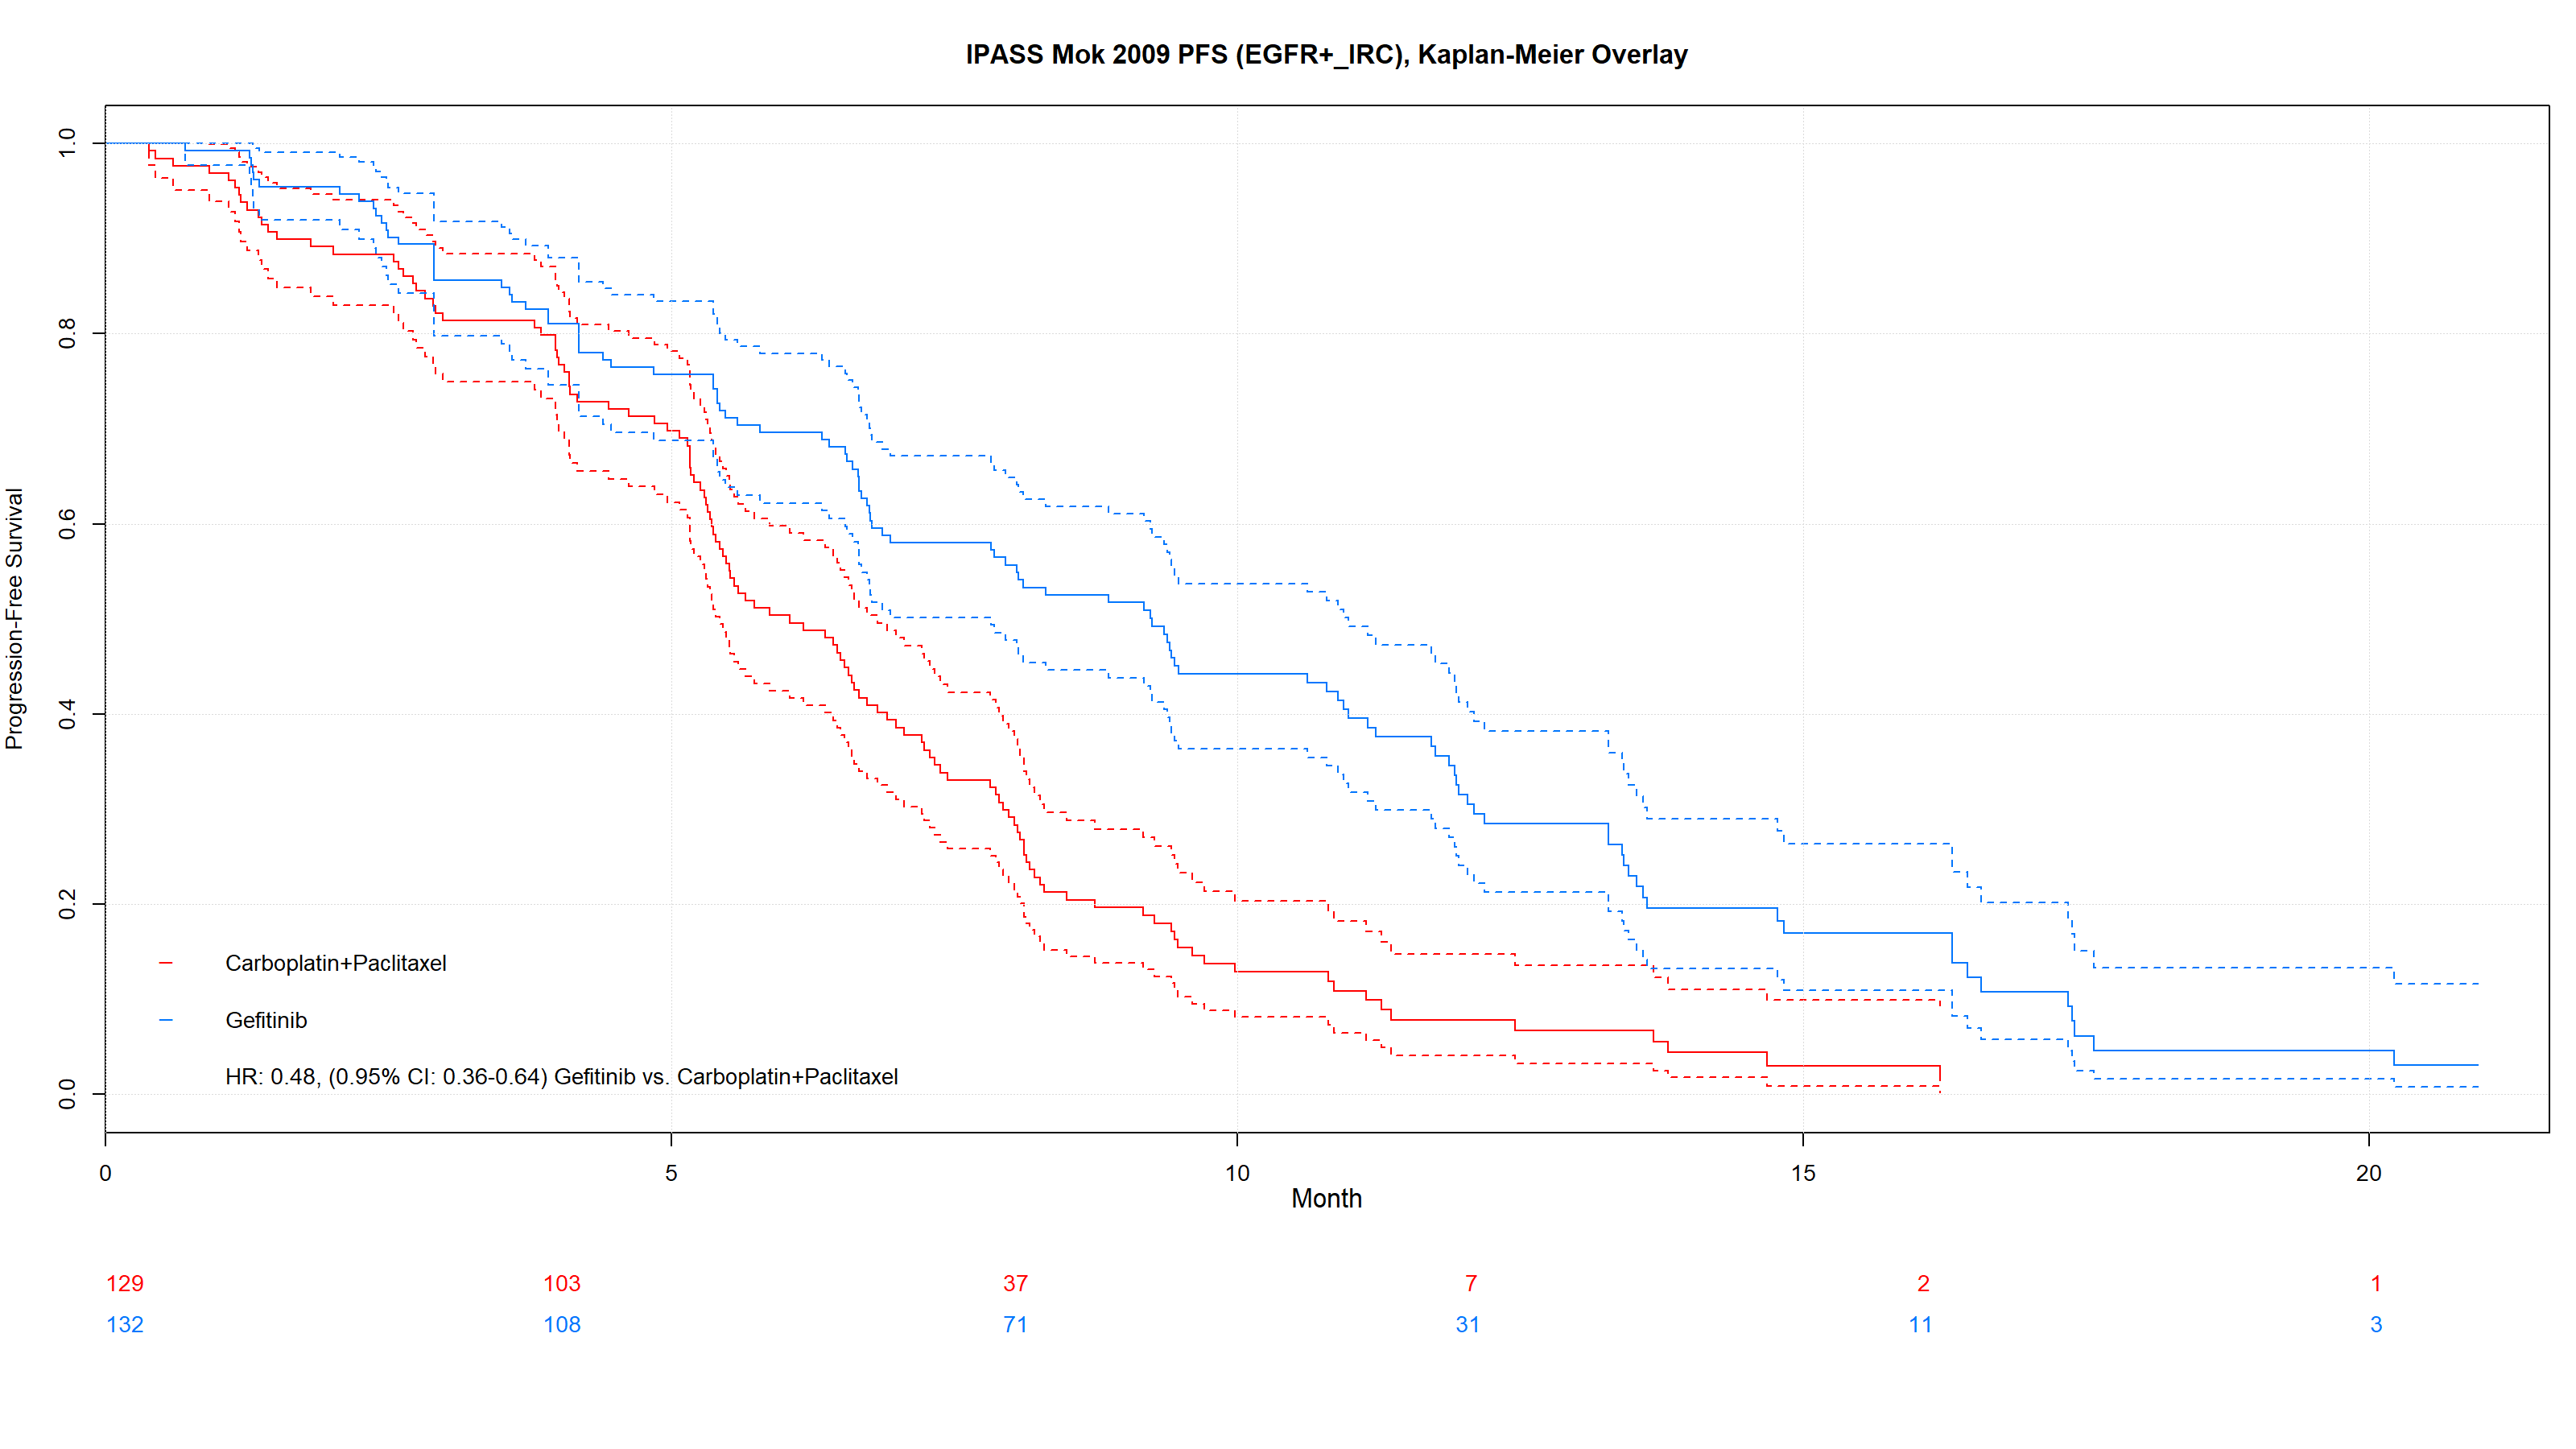
\includegraphics[max size={\textwidth}{\textheight}]{figs/km-plots/IPASS Mok 2009 PFS (EGFR+_IRC) Kaplan Meier.png}
\end{subfigure}
\begin{subfigure}{\textwidth}
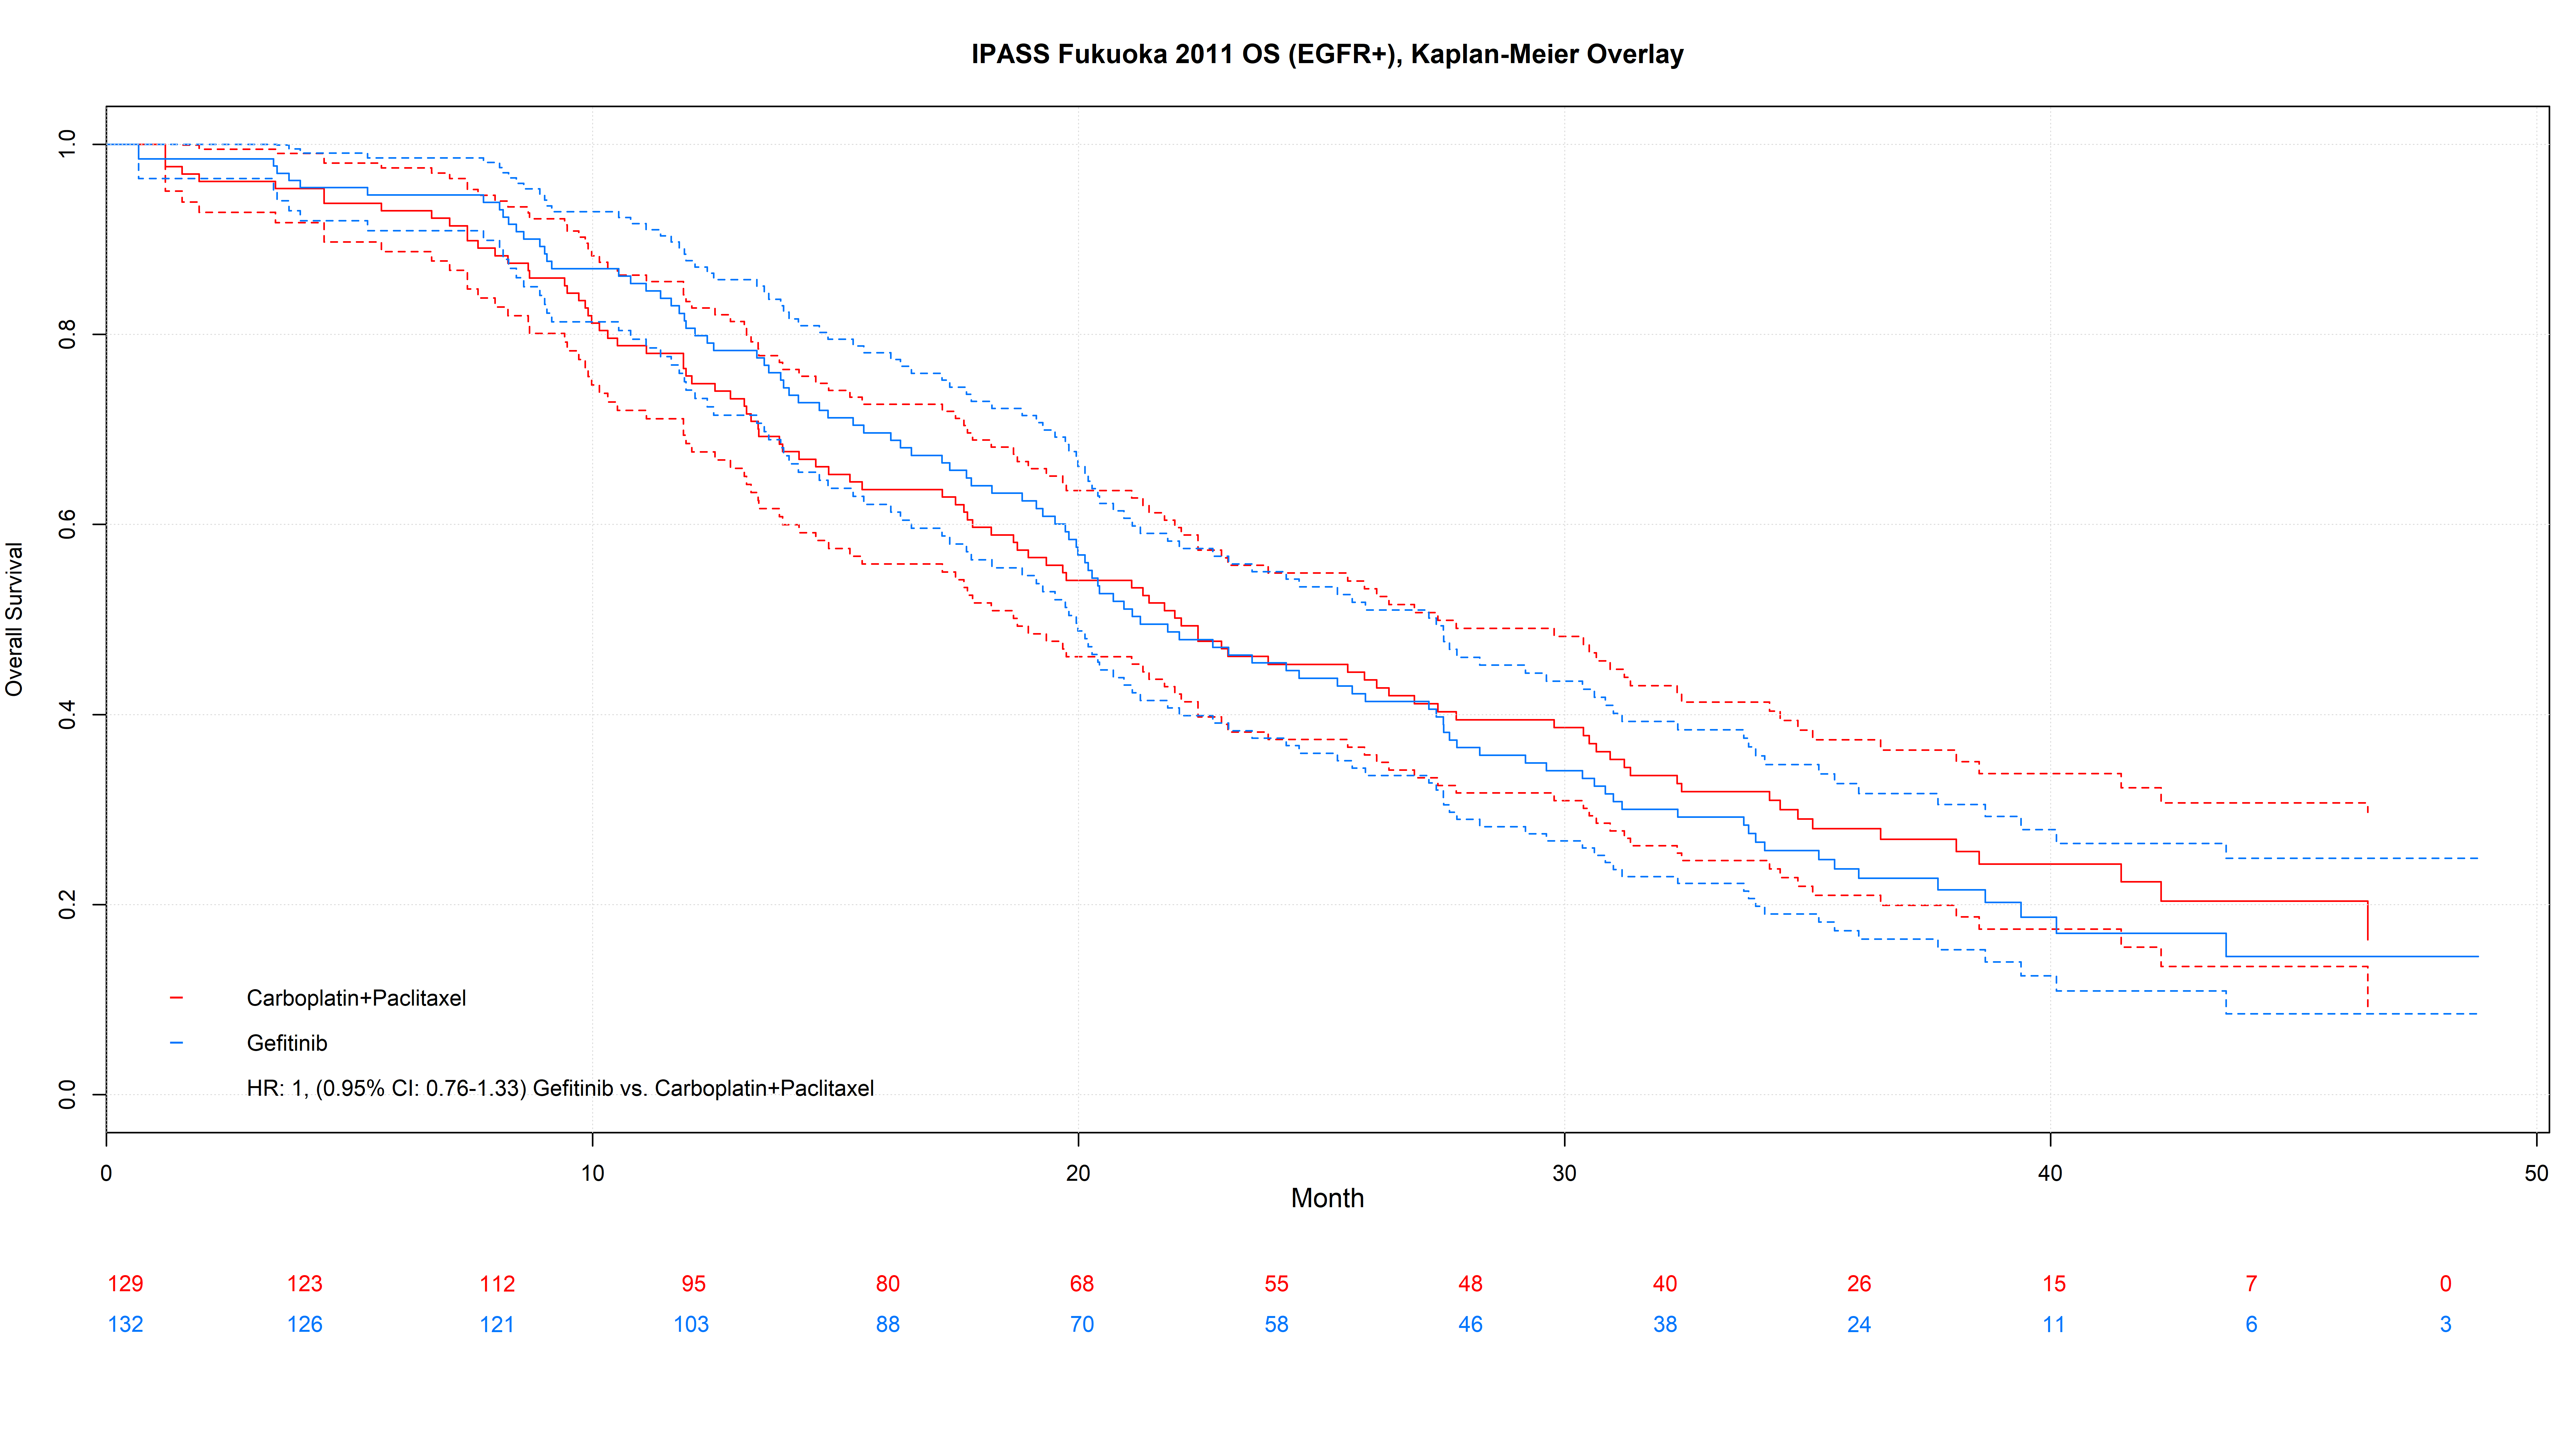
\includegraphics[max size={\textwidth}{\textheight}]{figs/km-plots/IPASS Fukuoka 2011 OS (EGFR+) Kaplan Meier.png}
\end{subfigure}
\centering
\caption{IPASS, progression-free survival and overall survival}\label{fig:IPASS}
\end{figure}


\begin{figure}
\centering
\begin{subfigure}{\textwidth}
\centering
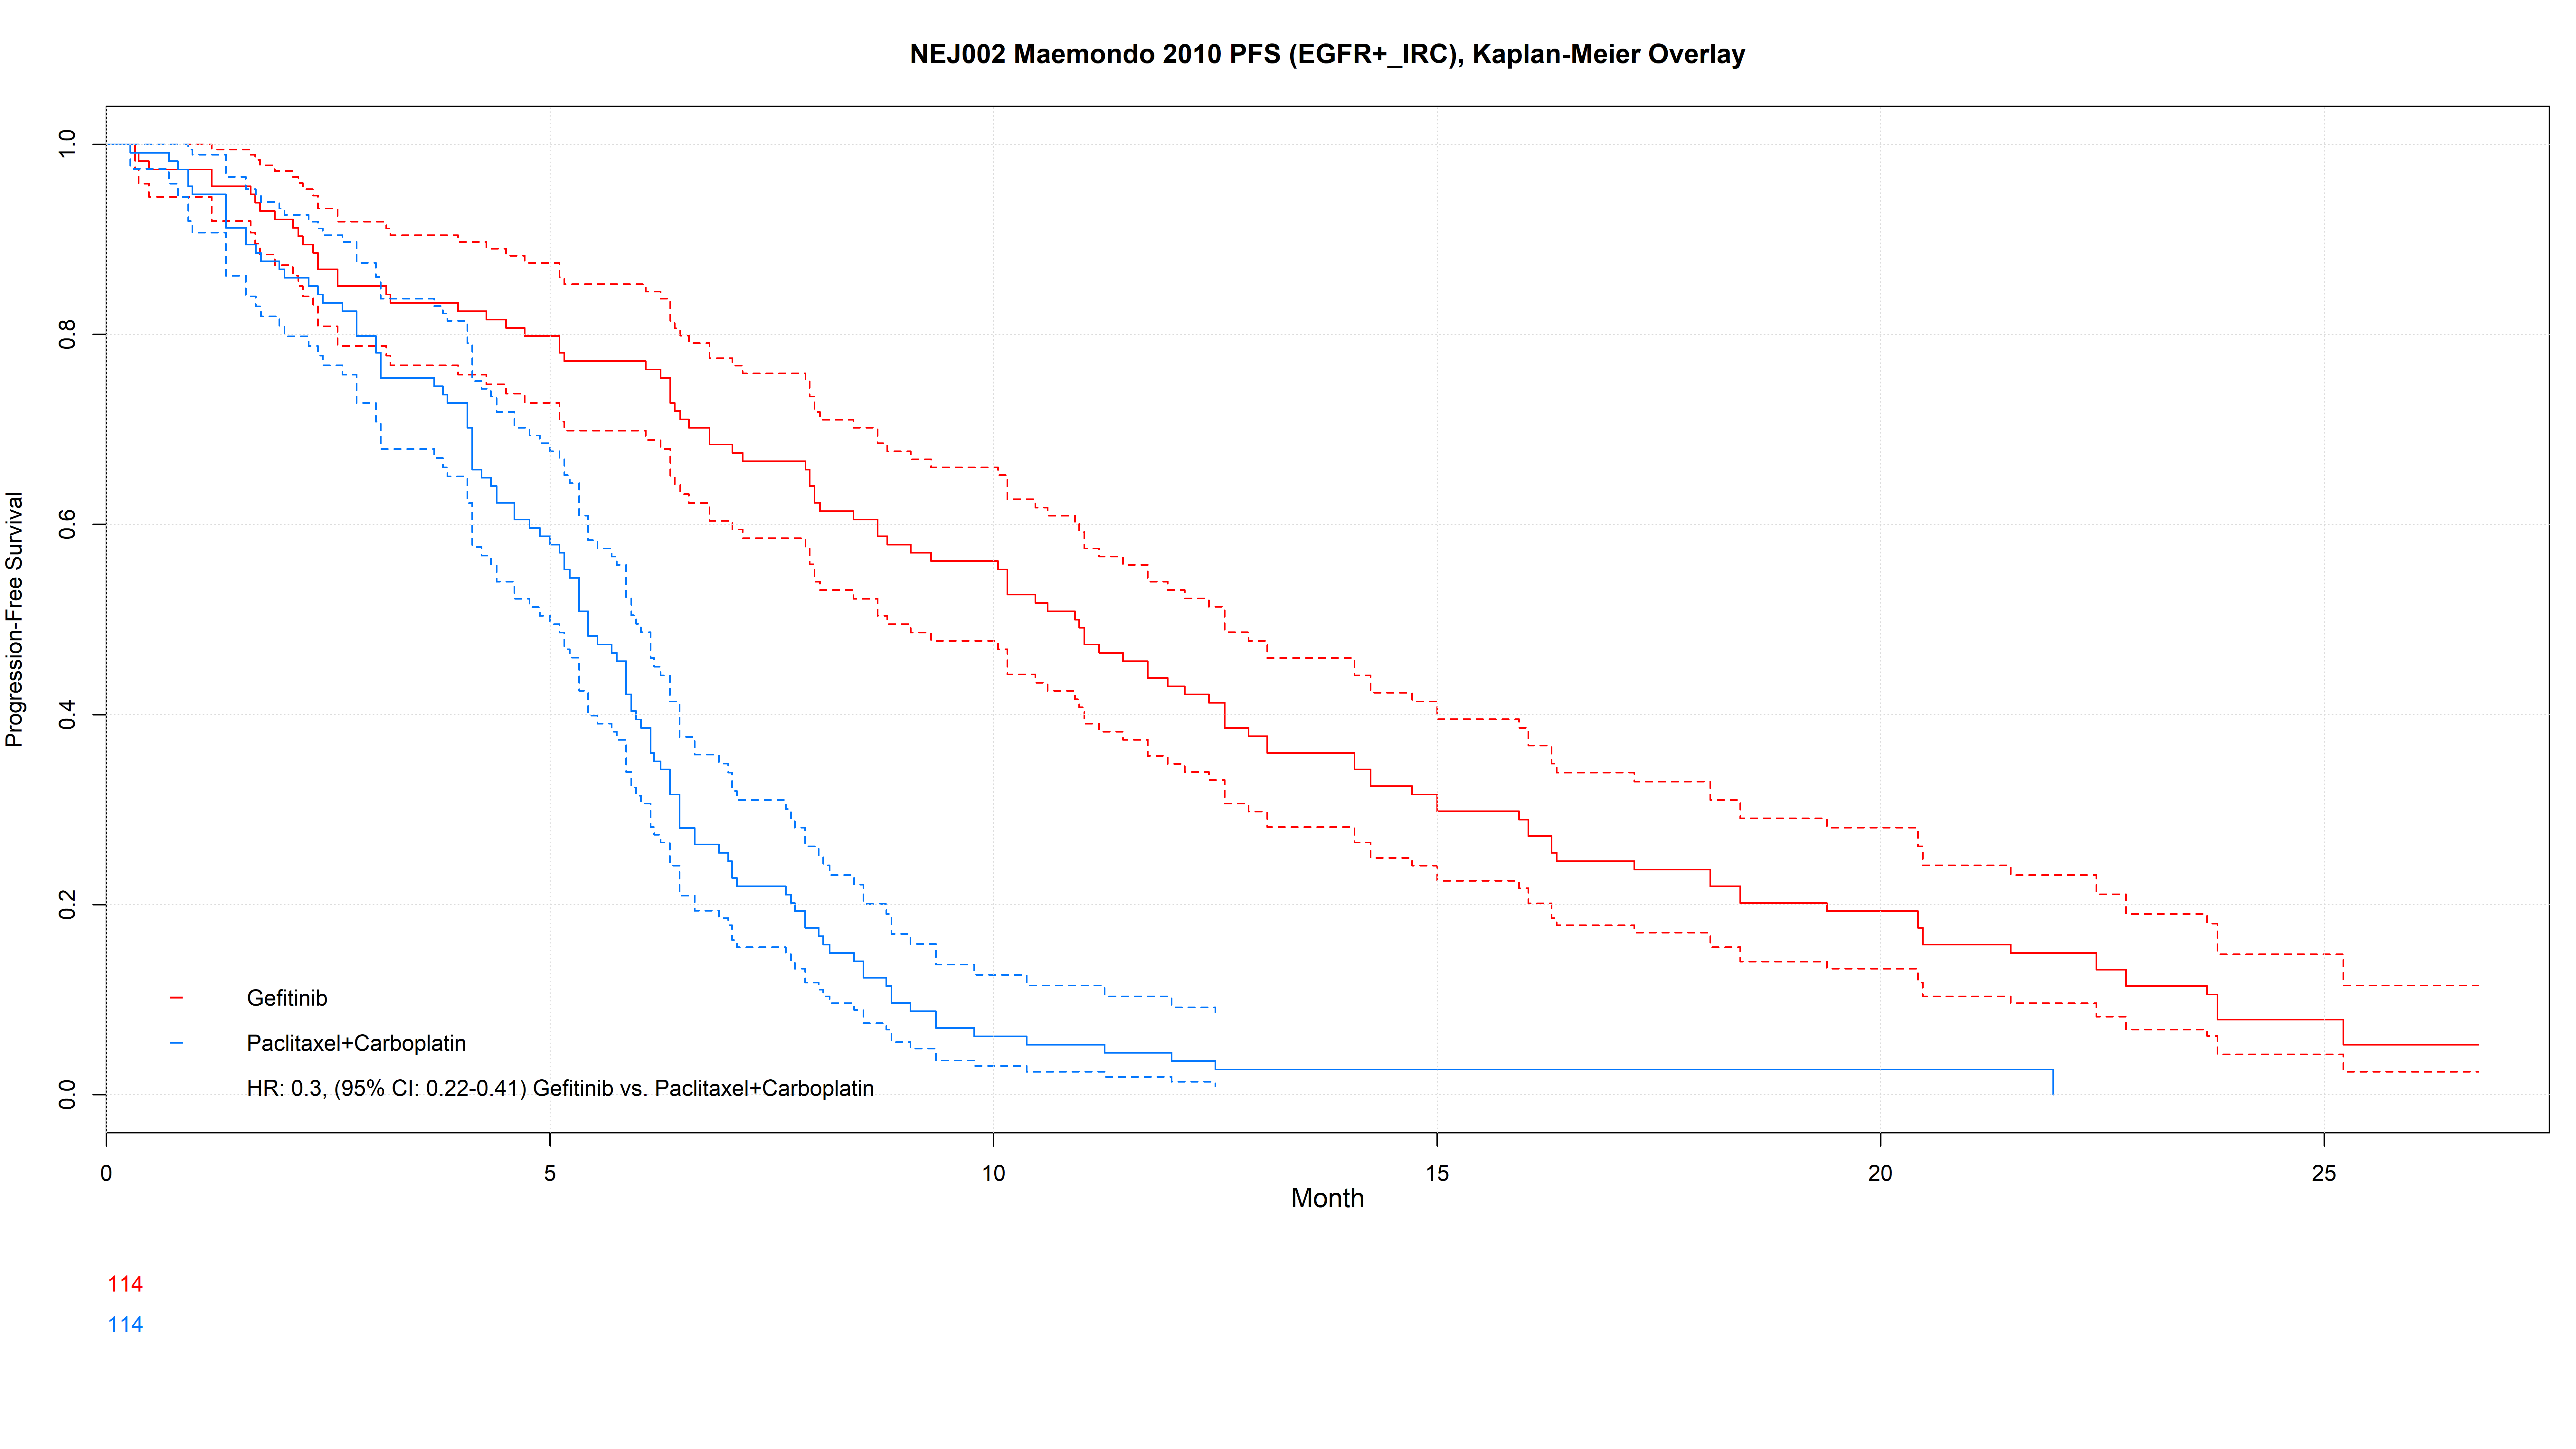
\includegraphics[max size={\textwidth}{\textheight}]{figs/km-plots/NEJ002 Maemondo 2010 PFS (EGFR+_IRC) Kaplan Meier.png}
\end{subfigure}
\begin{subfigure}{\textwidth}
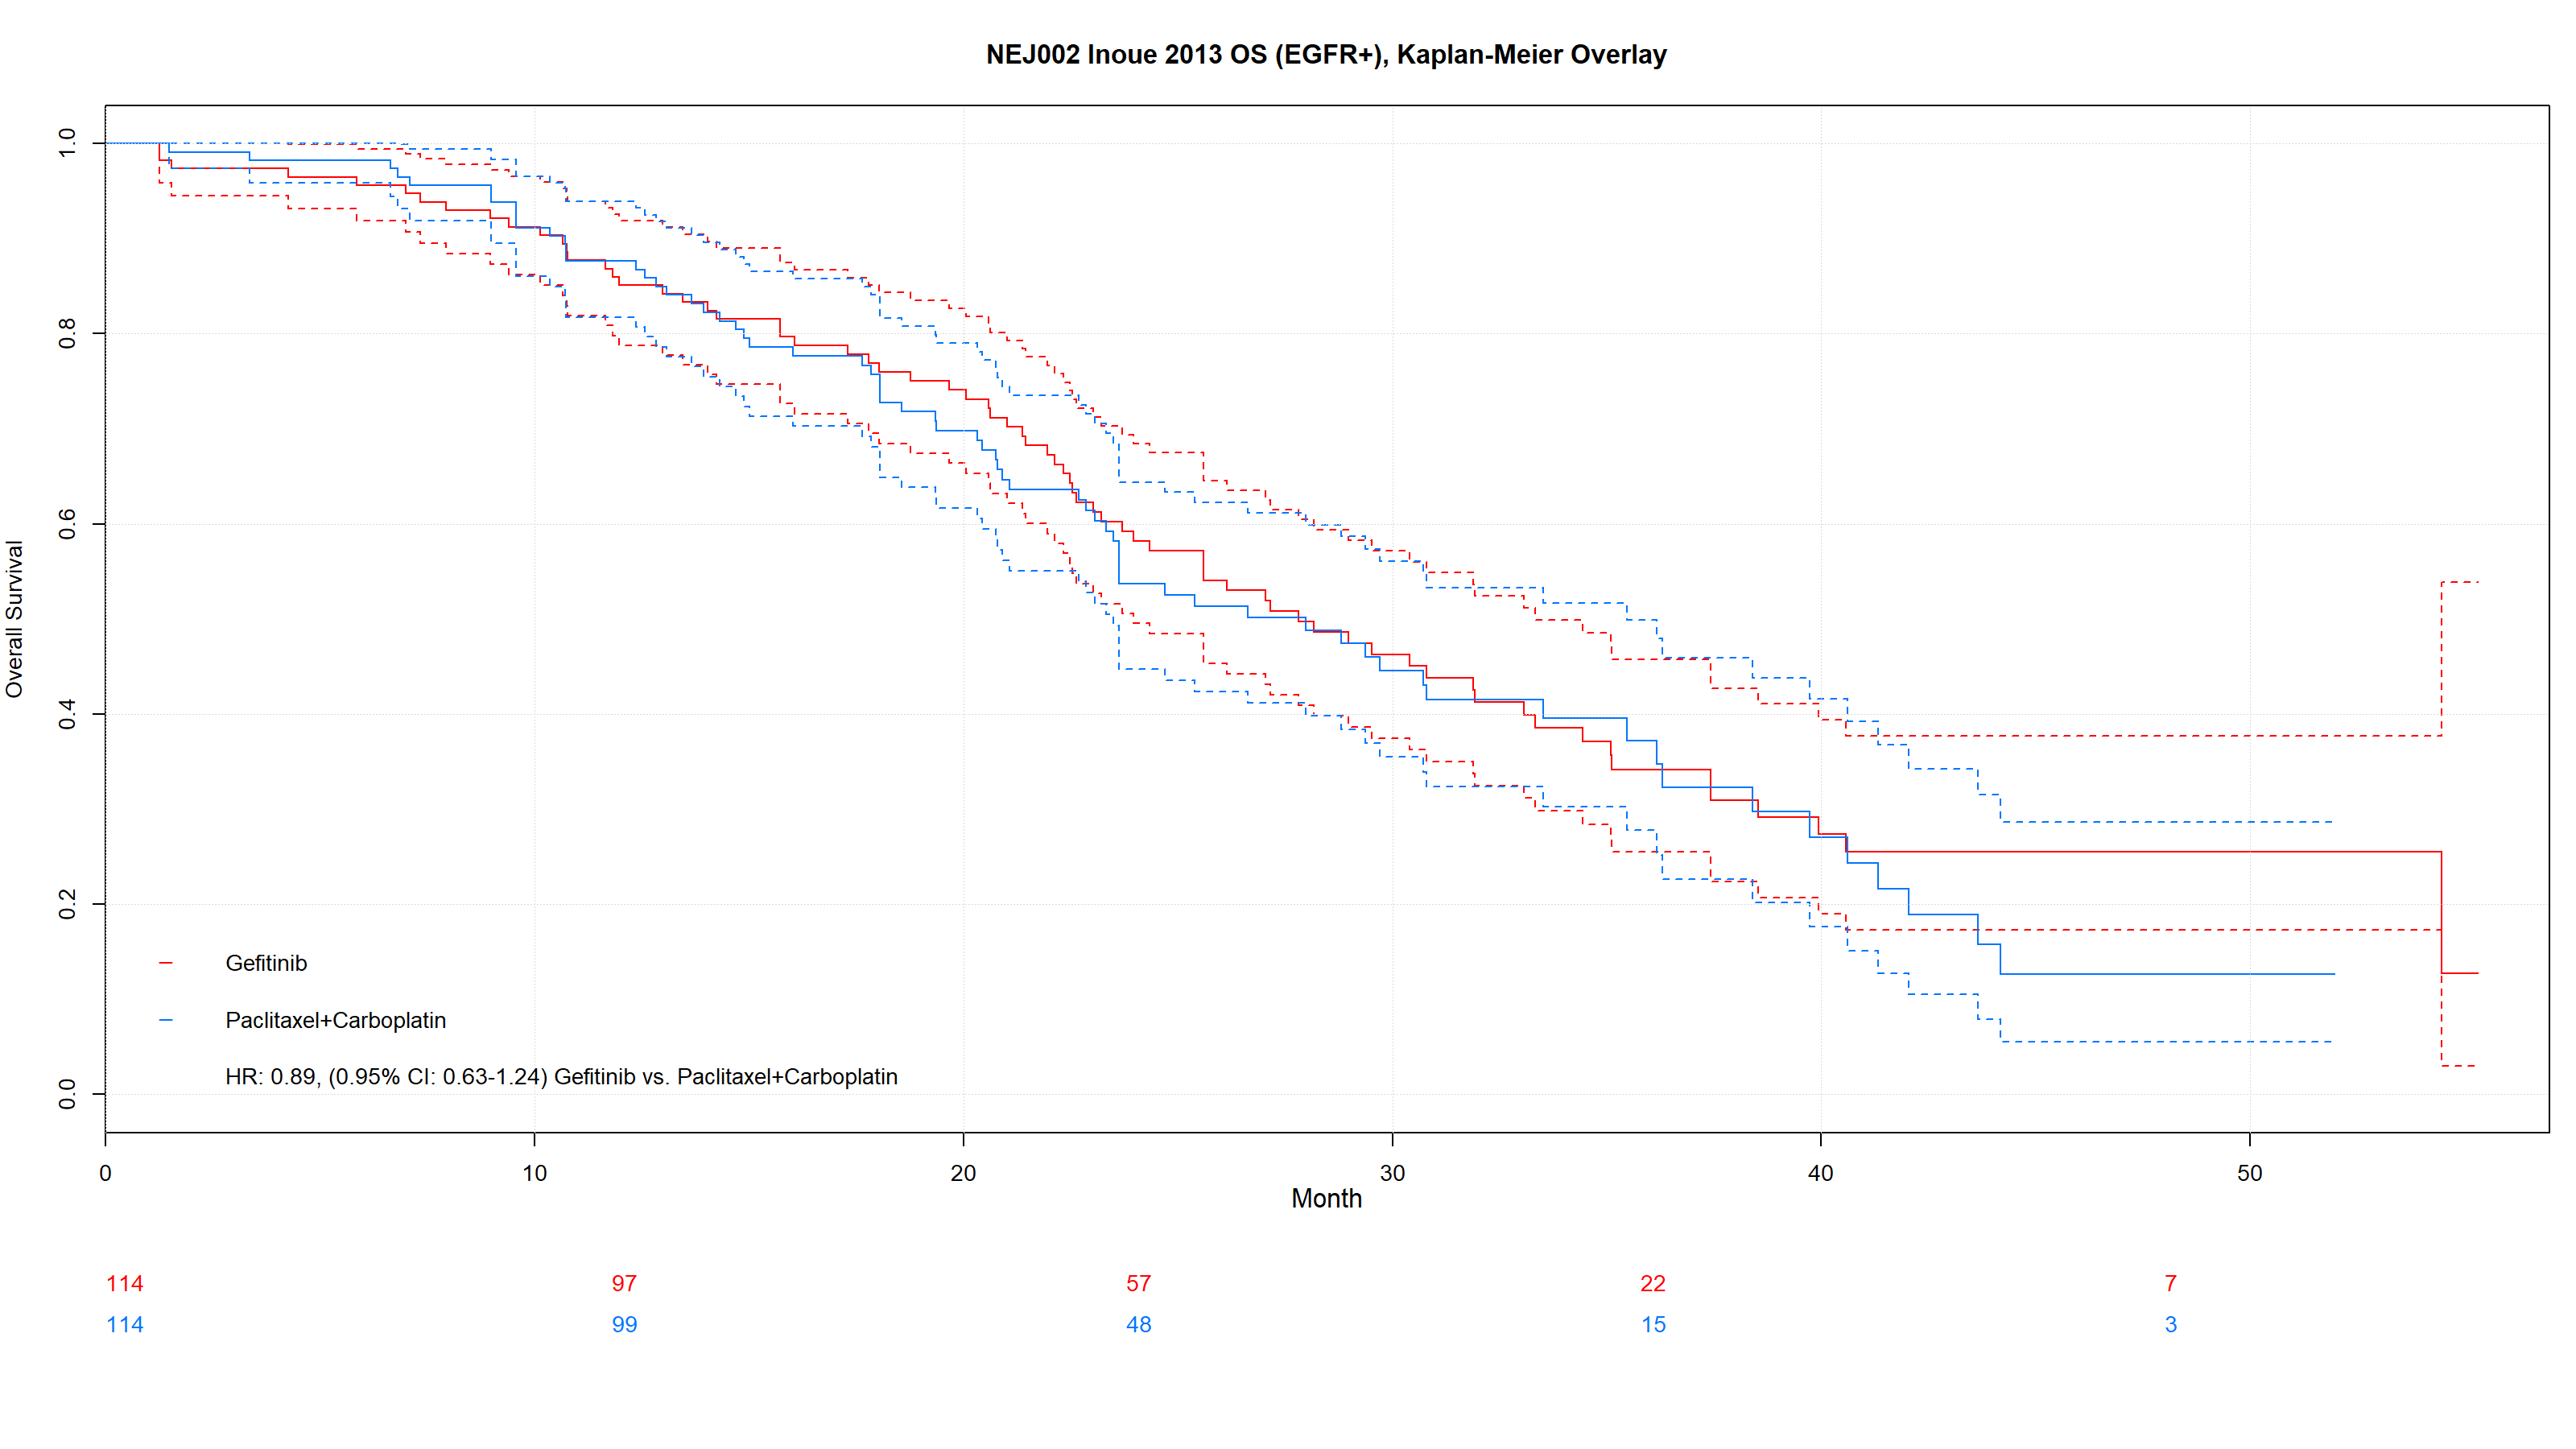
\includegraphics[max size={\textwidth}{\textheight}]{figs/km-plots/NEJ002 Inoue 2013 OS (EGFR+) Kaplan Meier.png}
\end{subfigure}
\centering
\caption{NEJ002, progression-free survival and overall survival}\label{fig:NEJ002}
\end{figure}



\begin{figure}
\centering
\begin{subfigure}{\textwidth}
\centering
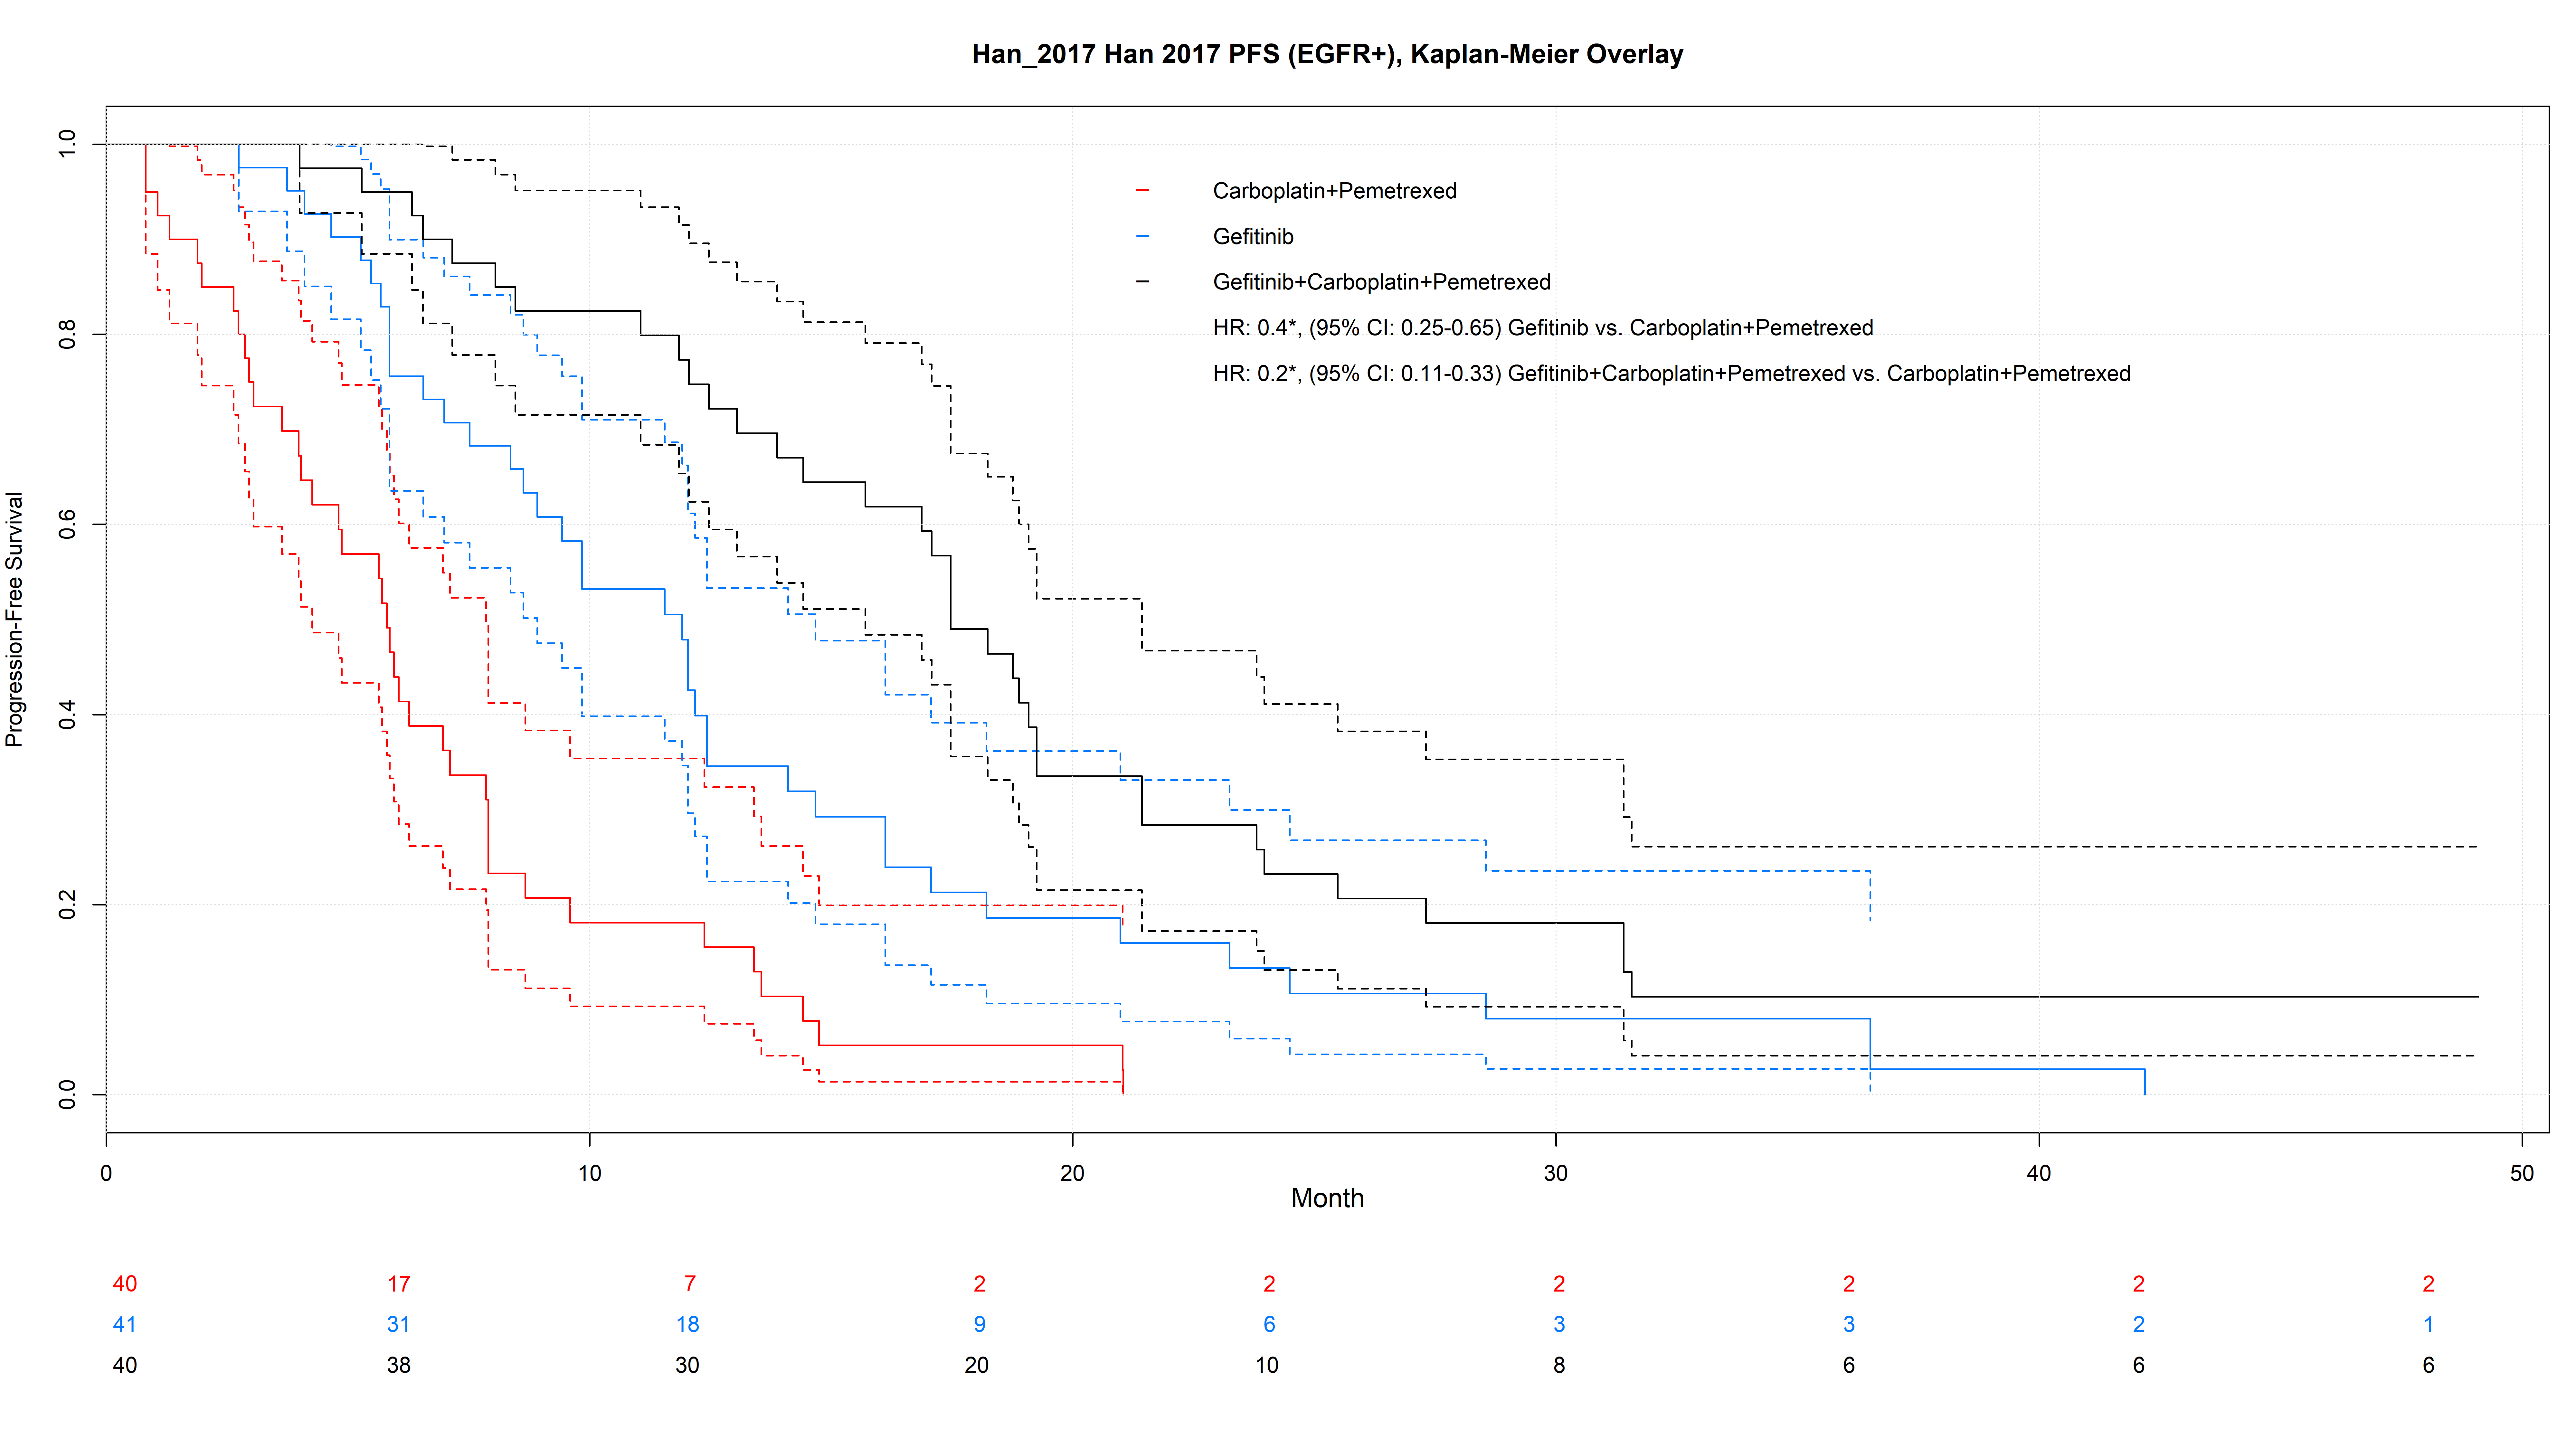
\includegraphics[max size={\textwidth}{\textheight}]{figs/km-plots/Han_2017 Han 2017 PFS (EGFR+) Kaplan Meier.png}
\end{subfigure}
\begin{subfigure}{\textwidth}
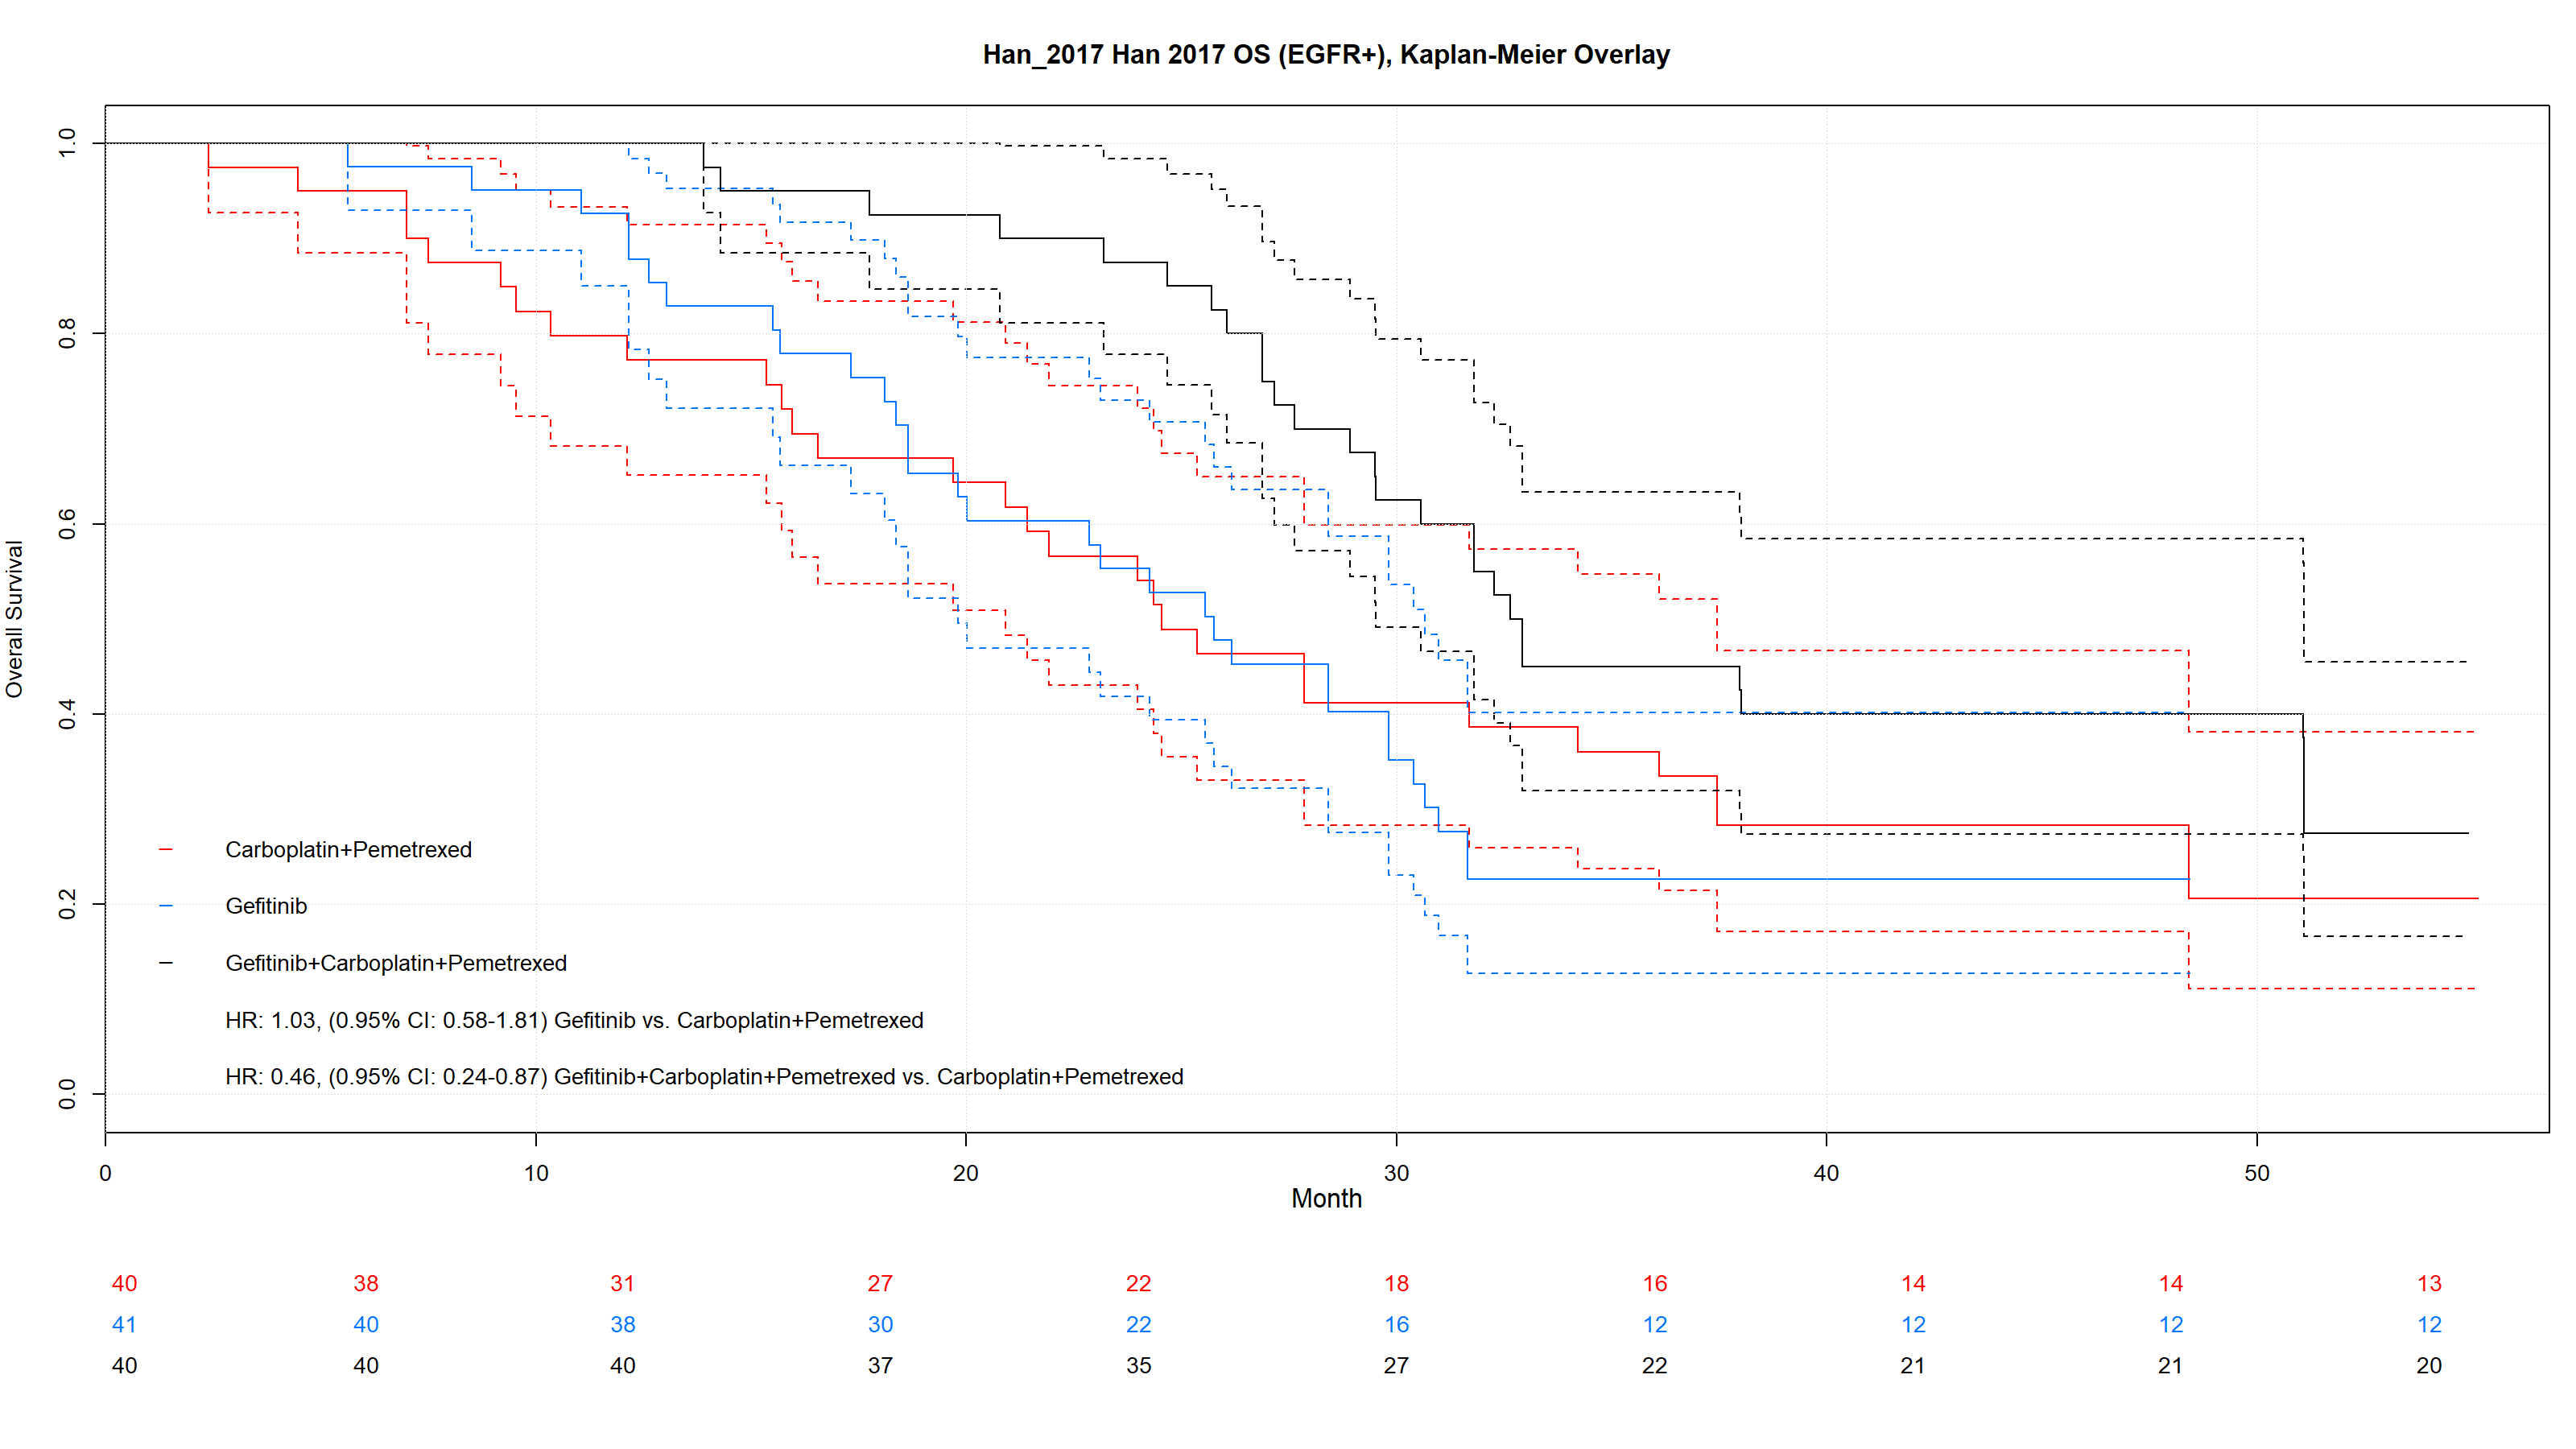
\includegraphics[max size={\textwidth}{\textheight}]{figs/km-plots/Han_2017 Han 2017 OS (EGFR+) Kaplan Meier.png}
\end{subfigure}
\centering
\caption{Han 2017, progression-free survival and overall survival}\label{fig:Han-2017}
\end{figure}



\begin{figure}
\centering
\begin{subfigure}{\textwidth}
\centering
\includegraphics[max size={\textwidth}{\textheight}]{figs/km-plots/Yang_2014 Yang 2014 PFS (EGFR+) Kaplan Meier.png}
\end{subfigure}
\begin{subfigure}{\textwidth}
\includegraphics[max size={\textwidth}{\textheight}]{figs/km-plots/Yang_2014 Yang 2016 OS (EGFR+) Kaplan Meier.png}
\end{subfigure}
\centering
\caption{Yang 2014 and Yang 2016, progression-free survival and overall survival}\label{fig:Yang 2014}
\end{figure}


\subsubsection{2L treatment}

\begin{figure}
\centering
\includegraphics[max size={\textwidth}{\textheight}]{figs/km-plots/AURA3 Mok 2017 PFS (EGFR+_T790M+) Kaplan Meier.png}
\centering
\caption{AURA-3, progression-free survival with osimertinib (T790+)}\label{fig:osimertinib-2l-pfs}
\end{figure}

\begin{figure}
\centering
\begin{subfigure}{\textwidth}
\includegraphics[max size={\textwidth}{\textheight}]{figs/km-plots/AURA2 Mitsudomi 2017 OS (EGFR+_T790+) Kaplan Meier.png}
\end{subfigure}
\begin{subfigure}{\textwidth}
\includegraphics[max size={\textwidth}{\textheight}]{figs/km-plots/AURA_EXT Mitsudomi 2017 OS (EGFR+_T790+) Kaplan Meier.png}
\end{subfigure}
\centering
\caption{AURA-2 and AURA-ext, overall survival with osimertinib (T790+)}\label{fig:osimertinib-2l-os}
\end{figure}


\begin{figure}
\centering
\begin{subfigure}{\textwidth}
\centering
\includegraphics[max size={\textwidth}{\textheight}]{figs/km-plots/IMPRESS Soria 2015 PFS (EGFR+_IA) Kaplan Meier.png}
\end{subfigure}
\begin{subfigure}{\textwidth}
\includegraphics[max size={\textwidth}{\textheight}]{figs/km-plots/IMPRESS Mok 2017 OS (EGFR+) Kaplan Meier.png}
\end{subfigure}
\centering
\caption{IMPRESS, progression-free survival and overall survival with PBDC}\label{fig:Impress}
\end{figure}

\begin{figure}
\centering
\includegraphics[max size={\textwidth}{\textheight}]{figs/km-plots/AURA3 Mok 2017 PFS (EGFR+_IRC) Kaplan Meier.png}
\centering
\caption{AURA-3, progression-free survival with PBDC}\label{fig:Impress}
\end{figure}

\%fi




\section{Network meta-analysis for relative treatment effects with 1L therapy}
\subsection{JAGS code}\label{sec:1l-nma-jags}

\subsubsection{Fixed effects multistate Weibull and Gompertz network meta-analysis model for estimation of relative treatment effects with each treatment versus gefitinib} 

\begin{verbatim} 

model{
  #timepoints for which PFS and OS data is available
  for (i in 1:(Nd-207)){
    # likelihood
    r[i,1:3]~dmulti(p[i,1:3], z[i,1]) 
    r[i,4:6]~dmulti(p[i,4:6], z[i,2]) 
    r[i,7:9]~dmulti(p[i,7:9], z[i,3]) 
    
    p[i,1:3]~ddirch(alpha[])
    
    p[i,4]<-p[i,1]*exp(-(h.sd[i]+h.sp[i])*dt[i,1])
    p[i,5]<-p[i,2]*exp(-h.pd[i]*dt[i,1])+p[i,1]*h.sp[i]*(exp(-(h.sd[i]+h.sp[i])*dt[i,1])
    		-exp(-h.pd[i]*dt[i,1]))/(h.pd[i]-h.sp[i]-h.sd[i])
    p[i,6]<-1-(p[i,4]+p[i,5])
    
    p[i,7]<-p[i,1]*exp(-(h.sd[i]+h.sp[i])*dt[i,2])
    p[i,8]<-p[i,2]*exp(-h.pd[i]*dt[i,2])+p[i,1]*h.sp[i]*(exp(-(h.sd[i]+h.sp[i])*dt[i,2])
    		-exp(-h.pd[i]*dt[i,2]))/(h.pd[i]-h.sp[i]-h.sd[i])
    p[i,9]<-1-(p[i,7]+p[i,8])
    
    log(h.sp[i])<- Beta[s[i],a[i],1]+Beta[s[i],a[i],2]*timetrans1[i] 
    log(h.sd[i])<- Beta[s[i],a[i],3] 
    log(h.pd[i])<- Beta[s[i],a[i],4]+Beta[s[i],a[i],5]*timetrans1[i]
  }
  
 #timepoints for which only OS data is available (from studies with both PFS and OS)
   for (i in (Nd-206):Nd){
   # likelihood
    r_cond_surv[i]~dbinom(p_cond_surv[i], z_cond_surv[i]) 
    
    p_cond_surv[i]<-exp(-h.OS[i]*dt[i,2])
    h.OS[i]<-h.sd[i]+h.pd[i]
    
    log(h.sd[i])<- Beta[s[i],a[i],3] 
    log(h.pd[i])<- Beta[s[i],a[i],4]+Beta[s[i],a[i],5]*timetrans1[i]
  }
    
 
  #Fixed effects model
  for (l in 1:9){
    for (ll in 1:na[l]){
      Beta[l,ll,1]<-mu[l,1]+d[t[l,ll],1]-d[t[l,1],1]
      Beta[l,ll,2]<-mu[l,2]+d[t[l,ll],2]-d[t[l,1],2]
      Beta[l,ll,3]<-mu[l,3]
      Beta[l,ll,4]<-mu[l,4]+d[t[l,ll],3]-d[t[l,1],3]
      Beta[l,ll,5]<-mu[l,5]
    }
  }
  #FLAURA (Study 10 has a mixed control group, 66% GEF, 34% ERL)
  Beta[10,1,1]<-mu[10,1]
  Beta[10,1,2]<-mu[10,2]
  Beta[10,1,3]<-mu[10,3]
  Beta[10,1,4]<-mu[10,4]
  Beta[10,1,5]<-mu[10,5]
  
  Beta[10,2,1]<-mu[10,1]+d[5,1]-(0.66*d[1,1]+0.34*d[2,1])
  Beta[10,2,2]<-mu[10,2]+d[5,2]-(0.66*d[1,2]+0.34*d[2,2])
  Beta[10,2,3]<-mu[10,3]
  Beta[10,2,4]<-mu[10,4]+d[5,3]-(0.66*d[1,3]+0.34*d[2,3])
  Beta[10,2,5]<-mu[10,5]
  
  for (l in 11:Ns){
    for (ll in 1:na[l]){
      Beta[l,ll,1]<-mu[l,1]+d[t[l,ll],1]-d[t[l,1],1]
      Beta[l,ll,2]<-mu[l,2]+d[t[l,ll],2]-d[t[l,1],2]
      Beta[l,ll,3]<-mu[l,3]
      Beta[l,ll,4]<-mu[l,4]+d[t[l,ll],3]-d[t[l,1],3]
      Beta[l,ll,5]<-mu[l,5]
    }
  }
  
  #priors
  for (j in 1:Ns){
    mu[j,1:5] ~ dmnorm(prior_mean_mu[1:5],prior_varcov_mu[,]) 
  }
  
  d[1,1]<-0
  d[1,2]<-0
  d[1,3]<-0

  for (k in 2:Nt){
    d[k,1:3] ~ dmnorm(prior_mean_d[1:3],prior_varcov_d[,]) 
  }

}

\end{verbatim}

\subsubsection{Fixed effects multistate second order fractional polynomial network meta-analysis model for estimation of relative treatment effects of each treatment versus gefitinib}
\begin{verbatim} 

model{
  #timepoints for which PFS and OS data is available
  for (i in 1:(Nd-207)){
    # likelihood
    r[i,1:3]~dmulti(p[i,1:3], z[i,1]) 
    r[i,4:6]~dmulti(p[i,4:6], z[i,2]) 
    r[i,7:9]~dmulti(p[i,7:9], z[i,3]) 
    
    p[i,1:3]~ddirch(alpha[])
    
    p[i,4]<-p[i,1]*exp(-(h.sd[i]+h.sp[i])*dt[i,1])
    p[i,5]<-p[i,2]*exp(-h.pd[i]*dt[i,1])+p[i,1]*h.sp[i]*(exp(-(h.sd[i]+h.sp[i])*dt[i,1])
    		-exp(-h.pd[i]*dt[i,1]))/(h.pd[i]-h.sp[i]-h.sd[i])
    p[i,6]<-1-(p[i,4]+p[i,5])
    
    p[i,7]<-p[i,1]*exp(-(h.sd[i]+h.sp[i])*dt[i,2])
    p[i,8]<-p[i,2]*exp(-h.pd[i]*dt[i,2])+p[i,1]*h.sp[i]*(exp(-(h.sd[i]+h.sp[i])*dt[i,2])
    		-exp(-h.pd[i]*dt[i,2]))/(h.pd[i]-h.sp[i]-h.sd[i])
    p[i,9]<-1-(p[i,7]+p[i,8])
    
    log(h.sp[i])<- Beta[s[i],a[i],1]+Beta[s[i],a[i],2]*timetrans1[i]
    		+Beta[s[i],a[i],3]*timetrans2[i]
    log(h.sd[i])<- Beta[s[i],a[i],4] 
    log(h.pd[i])<- Beta[s[i],a[i],5]+Beta[s[i],a[i],6]*timetrans1[i]
  }
  
 #timepoints for which only OS data is available (from studies with both PFS and OS)
   for (i in (Nd-206):Nd){
   # likelihood
    r_cond_surv[i]~dbinom(p_cond_surv[i], z_cond_surv[i]) 
    
    p_cond_surv[i]<-exp(-h.OS[i]*dt[i,2])
    h.OS[i]<-h.sd[i]+h.pd[i]
    
    log(h.sd[i])<- Beta[s[i],a[i],4] 
    log(h.pd[i])<- Beta[s[i],a[i],5]+Beta[s[i],a[i],6]*timetrans1[i]
  }
    
 
  #Fixed effects model
  for (l in 1:9){
    for (ll in 1:na[l]){
      Beta[l,ll,1]<-mu[l,1]+d[t[l,ll],1]-d[t[l,1],1]
      Beta[l,ll,2]<-mu[l,2]+d[t[l,ll],2]-d[t[l,1],2]
      Beta[l,ll,3]<-mu[l,3]
      Beta[l,ll,4]<-mu[l,4]
      Beta[l,ll,5]<-mu[l,5]+d[t[l,ll],3]-d[t[l,1],3]
      Beta[l,ll,6]<-mu[l,6]
    }
  }
  #FLAURA (Study 10 has a mixed control group, 66% GEF, 34% ERL)
  Beta[10,1,1]<-mu[10,1]
  Beta[10,1,2]<-mu[10,2]
  Beta[10,1,3]<-mu[10,3]
  Beta[10,1,4]<-mu[10,4]
  Beta[10,1,5]<-mu[10,5]
  Beta[10,1,6]<-mu[10,6]
  
  Beta[10,2,1]<-mu[10,1]+d[5,1]-(0.66*d[1,1]+0.34*d[2,1])
  Beta[10,2,2]<-mu[10,2]+d[5,2]-(0.66*d[1,2]+0.34*d[2,2])
  Beta[10,2,3]<-mu[10,3]
  Beta[10,2,4]<-mu[10,4]
  Beta[10,2,5]<-mu[10,5]+d[5,3]-(0.66*d[1,3]+0.34*d[2,3])
  Beta[10,2,6]<-mu[10,6]
  
  for (l in 11:Ns){
    for (ll in 1:na[l]){
      Beta[l,ll,1]<-mu[l,1]+d[t[l,ll],1]-d[t[l,1],1]
      Beta[l,ll,2]<-mu[l,2]+d[t[l,ll],2]-d[t[l,1],2]
      Beta[l,ll,3]<-mu[l,3]
      Beta[l,ll,4]<-mu[l,4]
      Beta[l,ll,5]<-mu[l,5]+d[t[l,ll],3]-d[t[l,1],3]
      Beta[l,ll,6]<-mu[l,6]
    }
  }
  
  
  #priors
  for (j in 1:Ns){
    mu[j,1:6] ~ dmnorm(prior_mean_mu[1:6],prior_varcov_mu[,]) 
  }
  
  d[1,1]<-0
  d[1,2]<-0
  d[1,3]<-0

  for (k in 2:Nt){
    d[k,1:3] ~ dmnorm(prior_mean_d[1:3],prior_varcov_d[,]) 
  }
  
}

\end{verbatim}


\subsubsection{Random effects multistate Weibull and Gompertz network meta-analysis model for estimation of relative treatment effects of each treatment versus gefitinib}
\begin{verbatim} 

model{
  #timepoints for which PFS and OS data is available
  for (i in 1:(Nd-207)){
    # likelihood
    r[i,1:3]~dmulti(p[i,1:3], z[i,1]) 
    r[i,4:6]~dmulti(p[i,4:6], z[i,2]) 
    r[i,7:9]~dmulti(p[i,7:9], z[i,3]) 
    
    p[i,1:3]~ddirch(alpha[])
    
    p[i,4]<-p[i,1]*exp(-(h.sd[i]+h.sp[i])*dt[i,1])
    p[i,5]<-p[i,2]*exp(-h.pd[i]*dt[i,1])+p[i,1]*h.sp[i]*(exp(-(h.sd[i]+h.sp[i])*dt[i,1])
    		-exp(-h.pd[i]*dt[i,1]))/(h.pd[i]-h.sp[i]-h.sd[i])
    p[i,6]<-1-(p[i,4]+p[i,5])
    
    p[i,7]<-p[i,1]*exp(-(h.sd[i]+h.sp[i])*dt[i,2])
    p[i,8]<-p[i,2]*exp(-h.pd[i]*dt[i,2])+p[i,1]*h.sp[i]*(exp(-(h.sd[i]+h.sp[i])*dt[i,2])
    		-exp(-h.pd[i]*dt[i,2]))/(h.pd[i]-h.sp[i]-h.sd[i])
    p[i,9]<-1-(p[i,7]+p[i,8])
    
    log(h.sp[i])<- Beta[s[i],a[i],1]+Beta[s[i],a[i],2]*timetrans1[i] 
    log(h.sd[i])<- Beta[s[i],a[i],3] 
    log(h.pd[i])<- Beta[s[i],a[i],4]+Beta[s[i],a[i],5]*timetrans1[i]
  }
  
 #timepoints for which only OS data is available (from studies with both PFS and OS)
   for (i in (Nd-206):Nd){
   # likelihood
    r_cond_surv[i]~dbinom(p_cond_surv[i], z_cond_surv[i]) 
    
    p_cond_surv[i]<-exp(-h.OS[i]*dt[i,2])
    h.OS[i]<-h.sd[i]+h.pd[i]
    
    log(h.sd[i])<- Beta[s[i],a[i],3] 
    log(h.pd[i])<- Beta[s[i],a[i],4]+Beta[s[i],a[i],5]*timetrans1[i]
  }
    
 
  #Random effects model
  for (l in 1:Ns){
    w[l,1]<-0
    delta[l,1]<-0
  }
  
  for (l in 1:9){
    for (ll in 1:na[l]){
      Beta[l,ll,1]<-mu[l,1]+delta[l,ll]
      Beta[l,ll,2]<-mu[l,2]+d[t[l,ll],2]-d[t[l,1],2]
      Beta[l,ll,3]<-mu[l,3]
      Beta[l,ll,4]<-mu[l,4]+d[t[l,ll],3]-d[t[l,1],3]
      Beta[l,ll,5]<-mu[l,5]
    }
  }
  
  #FLAURA (Study 10 has a mixed control group, 66% GEF, 34% ERL)
  Beta[10,1,1]<-mu[10,1]
  Beta[10,1,2]<-mu[10,2]
  Beta[10,1,3]<-mu[10,3]
  Beta[10,1,4]<-mu[10,4]
  Beta[10,1,5]<-mu[10,5]
  
  Beta[10,2,1]<-mu[10,1]+delta[10,2]
  Beta[10,2,2]<-mu[10,2]+d[5,2]-(0.66*d[1,2]+0.34*d[2,2])
  Beta[10,2,3]<-mu[10,3]
  Beta[10,2,4]<-mu[10,4]+d[5,3]-(0.66*d[1,3]+0.34*d[2,3])
  Beta[10,2,5]<-mu[10,5]
  
  
  for (l in 11:Ns){
    for (ll in 1:na[l]){
      Beta[l,ll,1]<-mu[l,1]+delta[l,ll]
      Beta[l,ll,2]<-mu[l,2]+d[t[l,ll],2]-d[t[l,1],2]
      Beta[l,ll,3]<-mu[l,3]
      Beta[l,ll,4]<-mu[l,4]+d[t[l,ll],3]-d[t[l,1],3]
      Beta[l,ll,5]<-mu[l,5]
    }
  }

  

  for (l in 1:9){
    for (ll in 2:na[l]){
      delta[l,ll]~dnorm(md[l,ll],taud[l,ll])
      md[l,ll]<-d[t[l,ll],1]-d[t[l,1],1] +sw[l,ll]
      w[l,ll] <- (delta[l,ll] - d[t[l,ll],1] + d[t[l,1],1])
      sw[l,ll] <- sum(w[l,1:(ll-1)])/(ll-1) 
      taud[l,ll] <- tau *2*(ll-1)/ll 
    }
  }
  
  delta[10,2]~dnorm(md[10,2],taud[10,2])
  md[10,2]<-d[5,1]-(0.66*d[1,1]+0.34*d[2,1]) +sw[10,2]
  w[10,2] <- (delta[10,2] - d[5,1] + (0.66*d[1,1]+0.34*d[2,1]))
  sw[10,2] <- sum(w[10,1:(2-1)])/(2-1) 
  taud[10,2] <- tau *2*(2-1)/2 
  
  for (l in 11:Ns){
    for (ll in 2:na[l]){
      delta[l,ll]~dnorm(md[l,ll],taud[l,ll])
      md[l,ll]<-d[t[l,ll],1]-d[t[l,1],1] +sw[l,ll]
      w[l,ll] <- (delta[l,ll] - d[t[l,ll],1] + d[t[l,1],1])
      sw[l,ll] <- sum(w[l,1:(ll-1)])/(ll-1) 
      taud[l,ll] <- tau *2*(ll-1)/ll 
    }
  }
  
  
  #priors
  for (j in 1:Ns){
    mu[j,1:5] ~ dmnorm(prior_mean_mu[1:5],prior_varcov_mu[,]) 
  }
  
  d[1,1]<-0
  d[1,2]<-0
  d[1,3]<-0

  for (k in 2:Nt){
    d[k,1:3] ~ dmnorm(prior_mean_d[1:3],prior_varcov_d[,]) 
  }
  
  sd~dunif(0,2)
  tau<-1/(sd*sd)
  
}

\end{verbatim}

\subsubsection{Random effects multistate second order fractional polynomial network meta-analysis model for estimation of relative treatment effects of each treatment versus gefitinib}
\begin{verbatim} 

model{
  #timepoints for which PFS and OS data is available
  for (i in 1:(Nd-207)){
    # likelihood
    r[i,1:3]~dmulti(p[i,1:3], z[i,1]) 
    r[i,4:6]~dmulti(p[i,4:6], z[i,2]) 
    r[i,7:9]~dmulti(p[i,7:9], z[i,3]) 
    
    p[i,1:3]~ddirch(alpha[])
    
    p[i,4]<-p[i,1]*exp(-(h.sd[i]+h.sp[i])*dt[i,1])
    p[i,5]<-p[i,2]*exp(-h.pd[i]*dt[i,1])+p[i,1]*h.sp[i]*(exp(-(h.sd[i]+h.sp[i])*dt[i,1])
    		-exp(-h.pd[i]*dt[i,1]))/(h.pd[i]-h.sp[i]-h.sd[i])
    p[i,6]<-1-(p[i,4]+p[i,5])
    
    p[i,7]<-p[i,1]*exp(-(h.sd[i]+h.sp[i])*dt[i,2])
    p[i,8]<-p[i,2]*exp(-h.pd[i]*dt[i,2])+p[i,1]*h.sp[i]*(exp(-(h.sd[i]+h.sp[i])*dt[i,2])
    		-exp(-h.pd[i]*dt[i,2]))/(h.pd[i]-h.sp[i]-h.sd[i])
    p[i,9]<-1-(p[i,7]+p[i,8])
    
    log(h.sp[i])<- Beta[s[i],a[i],1]+Beta[s[i],a[i],2]*timetrans1[i]
    		+Beta[s[i],a[i],3]*timetrans2[i]
    log(h.sd[i])<- Beta[s[i],a[i],4] 
    log(h.pd[i])<- Beta[s[i],a[i],5]+Beta[s[i],a[i],6]*timetrans1[i]
  }
  
 #timepoints for which only OS data is available (from studies with both PFS and OS)
   for (i in (Nd-206):Nd){
   # likelihood
    r_cond_surv[i]~dbinom(p_cond_surv[i], z_cond_surv[i]) 
    
    p_cond_surv[i]<-exp(-h.OS[i]*dt[i,2])
    h.OS[i]<-h.sd[i]+h.pd[i]
    
    log(h.sd[i])<- Beta[s[i],a[i],4] 
    log(h.pd[i])<- Beta[s[i],a[i],5]+Beta[s[i],a[i],6]*timetrans1[i]
  }
    
 
  #Random effects model
  for (l in 1:Ns){
    w[l,1]<-0
    delta[l,1]<-0
  }
  
  for (l in 1:9){
    for (ll in 1:na[l]){
      Beta[l,ll,1]<-mu[l,1]+delta[l,ll]
      Beta[l,ll,2]<-mu[l,2]+d[t[l,ll],2]-d[t[l,1],2]
      Beta[l,ll,3]<-mu[l,3]
      Beta[l,ll,4]<-mu[l,4]
      Beta[l,ll,5]<-mu[l,5]+d[t[l,ll],3]-d[t[l,1],3]
      Beta[l,ll,6]<-mu[l,6]
    }
  }
  
  #FLAURA (Study 10 has a mixed control group, 66% GEF, 34% ERL)
  Beta[10,1,1]<-mu[10,1]
  Beta[10,1,2]<-mu[10,2]
  Beta[10,1,3]<-mu[10,3]
  Beta[10,1,4]<-mu[10,4]
  Beta[10,1,5]<-mu[10,5]
  Beta[10,1,6]<-mu[10,6]
  
  Beta[10,2,1]<-mu[10,1]+delta[10,2]
  Beta[10,2,2]<-mu[10,2]+d[5,2]-(0.66*d[1,2]+0.34*d[2,2])
  Beta[10,2,3]<-mu[10,3]
  Beta[10,2,4]<-mu[10,4]
  Beta[10,2,5]<-mu[10,5]+d[5,3]-(0.66*d[1,3]+0.34*d[2,3])
  Beta[10,2,6]<-mu[10,6]
  
  
  for (l in 11:Ns){
    for (ll in 1:na[l]){
      Beta[l,ll,1]<-mu[l,1]+delta[l,ll]
      Beta[l,ll,2]<-mu[l,2]+d[t[l,ll],2]-d[t[l,1],2]
      Beta[l,ll,3]<-mu[l,3]
      Beta[l,ll,4]<-mu[l,4]
      Beta[l,ll,5]<-mu[l,5]+d[t[l,ll],3]-d[t[l,1],3]
      Beta[l,ll,6]<-mu[l,6]
    }
  }
  
  
  for (l in 1:9){
    for (ll in 2:na[l]){
      delta[l,ll]~dnorm(md[l,ll],taud[l,ll])
      md[l,ll]<-d[t[l,ll],1]-d[t[l,1],1] +sw[l,ll]
      w[l,ll] <- (delta[l,ll] - d[t[l,ll],1] + d[t[l,1],1])
      sw[l,ll] <- sum(w[l,1:(ll-1)])/(ll-1) 
      taud[l,ll] <- tau *2*(ll-1)/ll 
    }
  }
  
  delta[10,2]~dnorm(md[10,2],taud[10,2])
  md[10,2]<-d[5,1]-(0.66*d[1,1]+0.34*d[2,1]) +sw[10,2]
  w[10,2] <- (delta[10,2] - d[5,1] + (0.66*d[1,1]+0.34*d[2,1]))
  sw[10,2] <- sum(w[10,1:(2-1)])/(2-1) 
  taud[10,2] <- tau *2*(2-1)/2 
  
  for (l in 11:Ns){
    for (ll in 2:na[l]){
      delta[l,ll]~dnorm(md[l,ll],taud[l,ll])
      md[l,ll]<-d[t[l,ll],1]-d[t[l,1],1] +sw[l,ll]
      w[l,ll] <- (delta[l,ll] - d[t[l,ll],1] + d[t[l,1],1])
      sw[l,ll] <- sum(w[l,1:(ll-1)])/(ll-1) 
      taud[l,ll] <- tau *2*(ll-1)/ll 
    }
  }
  
  
  #priors
  for (j in 1:Ns){
    mu[j,1:6] ~ dmnorm(prior_mean_mu[1:6],prior_varcov_mu[,]) 
  }
  
  d[1,1]<-0
  d[1,2]<-0
  d[1,3]<-0

  for (k in 2:Nt){
    d[k,1:3] ~ dmnorm(prior_mean_d[1:3],prior_varcov_d[,]) 
  }
  
  sd~dunif(0,2)
  tau<-1/(sd*sd)
  
}

\end{verbatim}

\subsubsection{Fixed effects multistate Weibull and Gompertz network meta-analysis model for estimation of relative treatment effects of each treatment versus gefitinib; no treatment effect on PD transitions}
\begin{verbatim} 

model{
  #timepoints for which PFS and OS data is available
  for (i in 1:(Nd-207)){
    # likelihood
    r[i,1:3]~dmulti(p[i,1:3], z[i,1]) 
    r[i,4:6]~dmulti(p[i,4:6], z[i,2]) 
    r[i,7:9]~dmulti(p[i,7:9], z[i,3]) 
    
    p[i,1:3]~ddirch(alpha[])
    
    p[i,4]<-p[i,1]*exp(-(h.sd[i]+h.sp[i])*dt[i,1])
    p[i,5]<-p[i,2]*exp(-h.pd[i]*dt[i,1])+p[i,1]*h.sp[i]*(exp(-(h.sd[i]+h.sp[i])*dt[i,1])
    		-exp(-h.pd[i]*dt[i,1]))/(h.pd[i]-h.sp[i]-h.sd[i])
    p[i,6]<-1-(p[i,4]+p[i,5])
    
    p[i,7]<-p[i,1]*exp(-(h.sd[i]+h.sp[i])*dt[i,2])
    p[i,8]<-p[i,2]*exp(-h.pd[i]*dt[i,2])+p[i,1]*h.sp[i]*(exp(-(h.sd[i]+h.sp[i])*dt[i,2])
    		-exp(-h.pd[i]*dt[i,2]))/(h.pd[i]-h.sp[i]-h.sd[i])
    p[i,9]<-1-(p[i,7]+p[i,8])
    
    log(h.sp[i])<- Beta[s[i],a[i],1]+Beta[s[i],a[i],2]*timetrans1[i] 
    log(h.sd[i])<- Beta[s[i],a[i],3] 
    log(h.pd[i])<- Beta[s[i],a[i],4]+Beta[s[i],a[i],5]*timetrans1[i]
  }
  
 #timepoints for which only OS data is available (from studies with both PFS and OS)
   for (i in (Nd-206):Nd){
   # likelihood
    r_cond_surv[i]~dbinom(p_cond_surv[i], z_cond_surv[i]) 
    
    p_cond_surv[i]<-exp(-h.OS[i]*dt[i,2])
    h.OS[i]<-h.sd[i]+h.pd[i]
    
    log(h.sd[i])<- Beta[s[i],a[i],3] 
    log(h.pd[i])<- Beta[s[i],a[i],4]+Beta[s[i],a[i],5]*timetrans1[i]
  }
    
 
  #Fixed effects model
  for (l in 1:9){
    for (ll in 1:na[l]){
      Beta[l,ll,1]<-mu[l,1]+d[t[l,ll],1]-d[t[l,1],1]
      Beta[l,ll,2]<-mu[l,2]+d[t[l,ll],2]-d[t[l,1],2]
      Beta[l,ll,3]<-mu[l,3]
      Beta[l,ll,4]<-mu[l,4]
      Beta[l,ll,5]<-mu[l,5]
    }
  }
  #FLAURA (Study 10 has a mixed control group, 66% GEF, 34% ERL)
  Beta[10,1,1]<-mu[10,1]
  Beta[10,1,2]<-mu[10,2]
  Beta[10,1,3]<-mu[10,3]
  Beta[10,1,4]<-mu[10,4]
  Beta[10,1,5]<-mu[10,5]
  
  Beta[10,2,1]<-mu[10,1]+d[5,1]-(0.66*d[1,1]+0.34*d[2,1])
  Beta[10,2,2]<-mu[10,2]+d[5,2]-(0.66*d[1,2]+0.34*d[2,2])
  Beta[10,2,3]<-mu[10,3]
  Beta[10,2,4]<-mu[10,4]
  Beta[10,2,5]<-mu[10,5]
  
  for (l in 11:Ns){
    for (ll in 1:na[l]){
      Beta[l,ll,1]<-mu[l,1]+d[t[l,ll],1]-d[t[l,1],1]
      Beta[l,ll,2]<-mu[l,2]+d[t[l,ll],2]-d[t[l,1],2]
      Beta[l,ll,3]<-mu[l,3]
      Beta[l,ll,4]<-mu[l,4]
      Beta[l,ll,5]<-mu[l,5]
    }
  }
  
  #priors
  for (j in 1:Ns){
    mu[j,1:5] ~ dmnorm(prior_mean_mu[1:5],prior_varcov_mu[,]) 
  }
  
  d[1,1]<-0
  d[1,2]<-0

  for (k in 2:Nt){
    d[k,1:2] ~ dmnorm(prior_mean_d[1:2],prior_varcov_d[,]) 
  }
  
  \end{verbatim}


\subsubsection{Fixed effects multistate second order fractional polynomial network meta-analysis model for estimation of relative treatment effects of each treatment versus gefitinib; no treatment effect on PD transitions}
\begin{verbatim} 

model{
  #timepoints for which PFS and OS data is available
  for (i in 1:(Nd-207)){
    # likelihood
    r[i,1:3]~dmulti(p[i,1:3], z[i,1]) 
    r[i,4:6]~dmulti(p[i,4:6], z[i,2]) 
    r[i,7:9]~dmulti(p[i,7:9], z[i,3]) 
    
    p[i,1:3]~ddirch(alpha[])
    
    p[i,4]<-p[i,1]*exp(-(h.sd[i]+h.sp[i])*dt[i,1])
    p[i,5]<-p[i,2]*exp(-h.pd[i]*dt[i,1])+p[i,1]*h.sp[i]*(exp(-(h.sd[i]+h.sp[i])*dt[i,1])
    		-exp(-h.pd[i]*dt[i,1]))/(h.pd[i]-h.sp[i]-h.sd[i])
    p[i,6]<-1-(p[i,4]+p[i,5])
    
    p[i,7]<-p[i,1]*exp(-(h.sd[i]+h.sp[i])*dt[i,2])
    p[i,8]<-p[i,2]*exp(-h.pd[i]*dt[i,2])+p[i,1]*h.sp[i]*(exp(-(h.sd[i]+h.sp[i])*dt[i,2])
    		-exp(-h.pd[i]*dt[i,2]))/(h.pd[i]-h.sp[i]-h.sd[i])
    p[i,9]<-1-(p[i,7]+p[i,8])
    
    log(h.sp[i])<- Beta[s[i],a[i],1]+Beta[s[i],a[i],2]*timetrans1[i]
    		+Beta[s[i],a[i],3]*timetrans2[i]
    log(h.sd[i])<- Beta[s[i],a[i],4] 
    log(h.pd[i])<- Beta[s[i],a[i],5]+Beta[s[i],a[i],6]*timetrans1[i]
  }
  
 #timepoints for which only OS data is available (from studies with both PFS and OS)
   for (i in (Nd-206):Nd){
   # likelihood
    r_cond_surv[i]~dbinom(p_cond_surv[i], z_cond_surv[i]) 
    
    p_cond_surv[i]<-exp(-h.OS[i]*dt[i,2])
    h.OS[i]<-h.sd[i]+h.pd[i]
    
    log(h.sd[i])<- Beta[s[i],a[i],4] 
    log(h.pd[i])<- Beta[s[i],a[i],5]+Beta[s[i],a[i],6]*timetrans1[i]
  }
    
 
  #Fixed effects model
  for (l in 1:9){
    for (ll in 1:na[l]){
      Beta[l,ll,1]<-mu[l,1]+d[t[l,ll],1]-d[t[l,1],1]
      Beta[l,ll,2]<-mu[l,2]+d[t[l,ll],2]-d[t[l,1],2]
      Beta[l,ll,3]<-mu[l,3]
      Beta[l,ll,4]<-mu[l,4]
      Beta[l,ll,5]<-mu[l,5]
      Beta[l,ll,6]<-mu[l,6]
    }
  }
  #FLAURA (Study 10 has a mixed control group, 66% GEF, 34% ERL)
  Beta[10,1,1]<-mu[10,1]
  Beta[10,1,2]<-mu[10,2]
  Beta[10,1,3]<-mu[10,3]
  Beta[10,1,4]<-mu[10,4]
  Beta[10,1,5]<-mu[10,5]
  Beta[10,1,6]<-mu[10,6]
  
  Beta[10,2,1]<-mu[10,1]+d[5,1]-(0.66*d[1,1]+0.34*d[2,1])
  Beta[10,2,2]<-mu[10,2]+d[5,2]-(0.66*d[1,2]+0.34*d[2,2])
  Beta[10,2,3]<-mu[10,3]
  Beta[10,2,4]<-mu[10,4]
  Beta[10,2,5]<-mu[10,5]
  Beta[10,2,6]<-mu[10,6]
  
  for (l in 11:Ns){
    for (ll in 1:na[l]){
      Beta[l,ll,1]<-mu[l,1]+d[t[l,ll],1]-d[t[l,1],1]
      Beta[l,ll,2]<-mu[l,2]+d[t[l,ll],2]-d[t[l,1],2]
      Beta[l,ll,3]<-mu[l,3]
      Beta[l,ll,4]<-mu[l,4]
      Beta[l,ll,5]<-mu[l,5]
      Beta[l,ll,6]<-mu[l,6]
    }
  }
  
  
  #priors
  for (j in 1:Ns){
    mu[j,1:6] ~ dmnorm(prior_mean_mu[1:6],prior_varcov_mu[,]) 
  }
  
  d[1,1]<-0
  d[1,2]<-0
  

  for (k in 2:Nt){
    d[k,1:2] ~ dmnorm(prior_mean_d[1:2],prior_varcov_d[,]) 
  }
  
}

\end{verbatim}

\subsubsection{Random effects multistate Weibull and Gompertz network meta-analysis model for estimation of relative treatment effects of each treatment versus gefitinib; no treatment effect on PD transitions}
\begin{verbatim} 

model{
  #timepoints for which PFS and OS data is available
  for (i in 1:(Nd-207)){
    # likelihood
    r[i,1:3]~dmulti(p[i,1:3], z[i,1]) 
    r[i,4:6]~dmulti(p[i,4:6], z[i,2]) 
    r[i,7:9]~dmulti(p[i,7:9], z[i,3]) 
    
    p[i,1:3]~ddirch(alpha[])
    
    p[i,4]<-p[i,1]*exp(-(h.sd[i]+h.sp[i])*dt[i,1])
    p[i,5]<-p[i,2]*exp(-h.pd[i]*dt[i,1])+p[i,1]*h.sp[i]*(exp(-(h.sd[i]+h.sp[i])*dt[i,1])
    		-exp(-h.pd[i]*dt[i,1]))/(h.pd[i]-h.sp[i]-h.sd[i])
    p[i,6]<-1-(p[i,4]+p[i,5])
    
    p[i,7]<-p[i,1]*exp(-(h.sd[i]+h.sp[i])*dt[i,2])
    p[i,8]<-p[i,2]*exp(-h.pd[i]*dt[i,2])+p[i,1]*h.sp[i]*(exp(-(h.sd[i]+h.sp[i])*dt[i,2])
    		-exp(-h.pd[i]*dt[i,2]))/(h.pd[i]-h.sp[i]-h.sd[i])
    p[i,9]<-1-(p[i,7]+p[i,8])
    
    log(h.sp[i])<- Beta[s[i],a[i],1]+Beta[s[i],a[i],2]*timetrans1[i] 
    log(h.sd[i])<- Beta[s[i],a[i],3] 
    log(h.pd[i])<- Beta[s[i],a[i],4]+Beta[s[i],a[i],5]*timetrans1[i]
  }
  
 #timepoints for which only OS data is available (from studies with both PFS and OS)
   for (i in (Nd-206):Nd){
   # likelihood
    r_cond_surv[i]~dbinom(p_cond_surv[i], z_cond_surv[i]) 
    
    p_cond_surv[i]<-exp(-h.OS[i]*dt[i,2])
    h.OS[i]<-h.sd[i]+h.pd[i]
    
    log(h.sd[i])<- Beta[s[i],a[i],3] 
    log(h.pd[i])<- Beta[s[i],a[i],4]+Beta[s[i],a[i],5]*timetrans1[i]
  }
    
 
  #Random effects model
  for (l in 1:Ns){
    w[l,1]<-0
    delta[l,1]<-0
  }
  
  for (l in 1:9){
    for (ll in 1:na[l]){
      Beta[l,ll,1]<-mu[l,1]+delta[l,ll]
      Beta[l,ll,2]<-mu[l,2]+d[t[l,ll],2]-d[t[l,1],2]
      Beta[l,ll,3]<-mu[l,3]
      Beta[l,ll,4]<-mu[l,4]
      Beta[l,ll,5]<-mu[l,5]
    }
  }
  
  #FLAURA (Study 10 has a mixed control group, 66% GEF, 34% ERL)
  Beta[10,1,1]<-mu[10,1]
  Beta[10,1,2]<-mu[10,2]
  Beta[10,1,3]<-mu[10,3]
  Beta[10,1,4]<-mu[10,4]
  Beta[10,1,5]<-mu[10,5]
  
  Beta[10,2,1]<-mu[10,1]+delta[10,2]
  Beta[10,2,2]<-mu[10,2]+d[5,2]-(0.66*d[1,2]+0.34*d[2,2])
  Beta[10,2,3]<-mu[10,3]
  Beta[10,2,4]<-mu[10,4]
  Beta[10,2,5]<-mu[10,5]
  
  
  for (l in 11:Ns){
    for (ll in 1:na[l]){
      Beta[l,ll,1]<-mu[l,1]+delta[l,ll]
      Beta[l,ll,2]<-mu[l,2]+d[t[l,ll],2]-d[t[l,1],2]
      Beta[l,ll,3]<-mu[l,3]
      Beta[l,ll,4]<-mu[l,4]
      Beta[l,ll,5]<-mu[l,5]
    }
  }

  
  for (l in 1:9){
    for (ll in 2:na[l]){
      delta[l,ll]~dnorm(md[l,ll],taud[l,ll])
      md[l,ll]<-d[t[l,ll],1]-d[t[l,1],1] +sw[l,ll]
      w[l,ll] <- (delta[l,ll] - d[t[l,ll],1] + d[t[l,1],1])
      sw[l,ll] <- sum(w[l,1:(ll-1)])/(ll-1) 
      taud[l,ll] <- tau *2*(ll-1)/ll 
    }
  }
  
  delta[10,2]~dnorm(md[10,2],taud[10,2])
  md[10,2]<-d[5,1]-(0.66*d[1,1]+0.34*d[2,1]) +sw[10,2]
  w[10,2] <- (delta[10,2] - d[5,1] + (0.66*d[1,1]+0.34*d[2,1]))
  sw[10,2] <- sum(w[10,1:(2-1)])/(2-1) 
  taud[10,2] <- tau *2*(2-1)/2 
  
  for (l in 11:Ns){
    for (ll in 2:na[l]){
      delta[l,ll]~dnorm(md[l,ll],taud[l,ll])
      md[l,ll]<-d[t[l,ll],1]-d[t[l,1],1] +sw[l,ll]
      w[l,ll] <- (delta[l,ll] - d[t[l,ll],1] + d[t[l,1],1])
      sw[l,ll] <- sum(w[l,1:(ll-1)])/(ll-1) 
      taud[l,ll] <- tau *2*(ll-1)/ll 
    }
  }
  
  
  #priors
  for (j in 1:Ns){
    mu[j,1:5] ~ dmnorm(prior_mean_mu[1:5],prior_varcov_mu[,]) 
  }
  
  d[1,1]<-0
  d[1,2]<-0


  for (k in 2:Nt){
    d[k,1:2] ~ dmnorm(prior_mean_d[1:2],prior_varcov_d[,]) 
  }
  
  sd~dunif(0,2)
  tau<-1/(sd*sd)
  
}

\end{verbatim}

\subsubsection{Random effects multistate second order fractional polynomial network meta-analysis model for estimation of relative treatment effects of each treatment versus gefitinib; no treatment effect on PD transitions}
\begin{verbatim} 

model{
  #timepoints for which PFS and OS data is available
  for (i in 1:(Nd-207)){
    # likelihood
    r[i,1:3]~dmulti(p[i,1:3], z[i,1]) 
    r[i,4:6]~dmulti(p[i,4:6], z[i,2]) 
    r[i,7:9]~dmulti(p[i,7:9], z[i,3]) 
    
    p[i,1:3]~ddirch(alpha[])
    
    p[i,4]<-p[i,1]*exp(-(h.sd[i]+h.sp[i])*dt[i,1])
    p[i,5]<-p[i,2]*exp(-h.pd[i]*dt[i,1])+p[i,1]*h.sp[i]*(exp(-(h.sd[i]+h.sp[i])*dt[i,1])
    		-exp(-h.pd[i]*dt[i,1]))/(h.pd[i]-h.sp[i]-h.sd[i])
    p[i,6]<-1-(p[i,4]+p[i,5])
    
    p[i,7]<-p[i,1]*exp(-(h.sd[i]+h.sp[i])*dt[i,2])
    p[i,8]<-p[i,2]*exp(-h.pd[i]*dt[i,2])+p[i,1]*h.sp[i]*(exp(-(h.sd[i]+h.sp[i])*dt[i,2])
    		-exp(-h.pd[i]*dt[i,2]))/(h.pd[i]-h.sp[i]-h.sd[i])
    p[i,9]<-1-(p[i,7]+p[i,8])
    
    log(h.sp[i])<- Beta[s[i],a[i],1]+Beta[s[i],a[i],2]*timetrans1[i]
    		+Beta[s[i],a[i],3]*timetrans2[i]
    log(h.sd[i])<- Beta[s[i],a[i],4] 
    log(h.pd[i])<- Beta[s[i],a[i],5]+Beta[s[i],a[i],6]*timetrans1[i]
  }
  
 #timepoints for which only OS data is available (from studies with both PFS and OS)
   for (i in (Nd-206):Nd){
   # likelihood
    r_cond_surv[i]~dbinom(p_cond_surv[i], z_cond_surv[i]) 
    
    p_cond_surv[i]<-exp(-h.OS[i]*dt[i,2])
    h.OS[i]<-h.sd[i]+h.pd[i]
    
    log(h.sd[i])<- Beta[s[i],a[i],4] 
    log(h.pd[i])<- Beta[s[i],a[i],5]+Beta[s[i],a[i],6]*timetrans1[i]
  }
    
 
  #Random effects model
  for (l in 1:Ns){
    w[l,1]<-0
    delta[l,1]<-0
  }
  
  for (l in 1:9){
    for (ll in 1:na[l]){
      Beta[l,ll,1]<-mu[l,1]+delta[l,ll]
      Beta[l,ll,2]<-mu[l,2]+d[t[l,ll],2]-d[t[l,1],2]
      Beta[l,ll,3]<-mu[l,3]
      Beta[l,ll,4]<-mu[l,4]
      Beta[l,ll,5]<-mu[l,5]
      Beta[l,ll,6]<-mu[l,6]
    }
  }
  
  #FLAURA (Study 10 has a mixed control group, 66% GEF, 34% ERL)
  Beta[10,1,1]<-mu[10,1]
  Beta[10,1,2]<-mu[10,2]
  Beta[10,1,3]<-mu[10,3]
  Beta[10,1,4]<-mu[10,4]
  Beta[10,1,5]<-mu[10,5]
  Beta[10,1,6]<-mu[10,6]
  
  Beta[10,2,1]<-mu[10,1]+delta[10,2]
  Beta[10,2,2]<-mu[10,2]+d[5,2]-(0.66*d[1,2]+0.34*d[2,2])
  Beta[10,2,3]<-mu[10,3]
  Beta[10,2,4]<-mu[10,4]
  Beta[10,2,5]<-mu[10,5]
  Beta[10,2,6]<-mu[10,6]
  
  
  for (l in 11:Ns){
    for (ll in 1:na[l]){
      Beta[l,ll,1]<-mu[l,1]+delta[l,ll]
      Beta[l,ll,2]<-mu[l,2]+d[t[l,ll],2]-d[t[l,1],2]
      Beta[l,ll,3]<-mu[l,3]
      Beta[l,ll,4]<-mu[l,4]
      Beta[l,ll,5]<-mu[l,5]
      Beta[l,ll,6]<-mu[l,6]
    }
  }
  
  
  for (l in 1:9){
    for (ll in 2:na[l]){
      delta[l,ll]~dnorm(md[l,ll],taud[l,ll])
      md[l,ll]<-d[t[l,ll],1]-d[t[l,1],1] +sw[l,ll]
      w[l,ll] <- (delta[l,ll] - d[t[l,ll],1] + d[t[l,1],1])
      sw[l,ll] <- sum(w[l,1:(ll-1)])/(ll-1) 
      taud[l,ll] <- tau *2*(ll-1)/ll 
    }
  }
  
  delta[10,2]~dnorm(md[10,2],taud[10,2])
  md[10,2]<-d[5,1]-(0.66*d[1,1]+0.34*d[2,1]) +sw[10,2]
  w[10,2] <- (delta[10,2] - d[5,1] + (0.66*d[1,1]+0.34*d[2,1]))
  sw[10,2] <- sum(w[10,1:(2-1)])/(2-1) 
  taud[10,2] <- tau *2*(2-1)/2 
  
  for (l in 11:Ns){
    for (ll in 2:na[l]){
      delta[l,ll]~dnorm(md[l,ll],taud[l,ll])
      md[l,ll]<-d[t[l,ll],1]-d[t[l,1],1] +sw[l,ll]
      w[l,ll] <- (delta[l,ll] - d[t[l,ll],1] + d[t[l,1],1])
      sw[l,ll] <- sum(w[l,1:(ll-1)])/(ll-1) 
      taud[l,ll] <- tau *2*(ll-1)/ll 
    }
  }
  
  
  #priors
  for (j in 1:Ns){
    mu[j,1:6] ~ dmnorm(prior_mean_mu[1:6],prior_varcov_mu[,]) 
  }
  
  d[1,1]<-0
  d[1,2]<-0

  for (k in 2:Nt){
    d[k,1:2] ~ dmnorm(prior_mean_d[1:2],prior_varcov_d[,]) 
  }
  
  sd~dunif(0,2)
  tau<-1/(sd*sd)
  
}

\end{verbatim}


\subsection{Model parameter estimates}

\begin{table}[!ht]
\begin{center}
\begin{threeparttable}
\footnotesize
\caption{First line relative treatment effects relative to gefitinib from the multi-state network meta-analysis}  \label{tbl:mstate-nma-1L-coef}
\begin{tabularx}{\textwidth}{@{\extracolsep{\fill}}llllrrrrr}
\hline
\multicolumn{4}{c}{} & \multicolumn{5}{c}{Posterior quantiles} \\
\cmidrule{5-9}
\multicolumn{1}{l}{Model} & \multicolumn{1}{l}{Transition} & \multicolumn{1}{l}{Coefficient} & \multicolumn{1}{l}{Treatment} 
& \multicolumn{1}{r}{2.5\%} & \multicolumn{1}{r}{25\%} & \multicolumn{1}{r}{50\%} & \multicolumn{1}{r}{75\%} & \multicolumn{1}{r}{97.5\%} \\
\hline
\ExpandableInput{tables/mstate-nma-1L-coef.txt}
\hline
\end{tabularx}
\scriptsize
\end{threeparttable}
\end{center}
\end{table}

\FloatBarrier

\subsection{Model fit}\label{app:DIC-nma-1l}

\begin{table}[!ht]
\begin{center}
\begin{threeparttable}
\footnotesize
\caption{Deviance information criterion for first line network meta-analysis } \label{tbl:dic-nma-1L}
\begin{tabularx}{\textwidth}{@{\extracolsep{\fill}}ld{-1}d{-1}d{-1}d{-1}}
\hline
\multicolumn{1}{l}{} & \multicolumn{2}{c}{Fixed effects} & \multicolumn{2}{c}{Random effects}\\
\cmidrule(r){2-3} \cmidrule(r){4-5}
\multicolumn{1}{l}{} & \multicolumn{1}{l}{Treatment effect} & \multicolumn{1}{l}{Treatment effect} & \multicolumn{1}{l}{Treatment effect} & \multicolumn{1}{l}{Treatment effect} \\
\multicolumn{1}{l}{} & \multicolumn{1}{l}{$P$ to $D$: none} & \multicolumn{1}{l}{$P$ to $D$: constant} & \multicolumn{1}{l}{$P$ to $D$: none} & \multicolumn{1}{l}{$P$ to $D$: constant} \\
\hline
\ExpandableInput{tables/dic-1L-nma.txt}
\hline
\end{tabularx}
\scriptsize
Notes: The transition from $P$ to $D$ is the transition from progression to death. If there is no treatment effect, then hazard rates do not vary across treatments or over time; if there is a constant treatment effect, then hazard rates vary across treatments but not over time.
\end{threeparttable}
\end{center}
\end{table}

\subsection{Supplementary figures of relative treatment effects}\label{app:nma-supp-figs}
\begin{figure}[h]
\centering
\includegraphics[max size={\textwidth}{\textheight}]{figs/hr-1L-weibull.pdf} 
\caption{First line estimates of hazard ratios from stable to progression relative to gefitinib from the multi-state network meta-analysis with a Weibull model}\label{fig:hr-1L-weibull}
\end{figure}

\begin{figure}[h]
\centering
\includegraphics[max size={\textwidth}{\textheight}]{figs/hr-1L-fp-00.pdf} 
\caption{First line estimates of hazard ratios from stable to progression relative to gefitinib from the multi-state network meta-analysis with a fractional polynomial (0, 0) model}\label{fig:hr-1L-fp-00}
\end{figure}

\begin{figure}[h]
\centering
\includegraphics[max size={\textwidth}{\textheight}]{figs/hr-1L-fp-01.pdf} 
\caption{First line estimates of hazard ratios from stable to progression relative to gefitinib from the multi-state network meta-analysis with a fractional polynomial (0, 1) model}\label{fig:hr-1L-fp-01}
\end{figure}

\begin{figure}
\centering
\includegraphics[max size={\textwidth}{\textheight}]{figs/hr-1L-gompertz.pdf} 
\caption{First line estimates of hazard ratios from stable to progression relative to gefitinib from the multi-state network meta-analysis with a Gompertz model}\label{fig:hr-1L-gompertz}
\end{figure}

\FloatBarrier

\section{Meta-analysis for absolute effects with 1L reference treatment}
\subsection{JAGS code}\label{sec:1l-ma-jags}

\subsubsection{Fixed effects multistate Weibull and Gompertz meta-analysis model for estimation of absolute effects with 1L gefitinib } 

\begin{verbatim} 

model{
 #timepoints for which PFS and OS data is available
  for (i in 1:(Nd-38)){
    # likelihood
    r[i,1:3]~dmulti(p[i,1:3], z[i,1]) 
    r[i,4:6]~dmulti(p[i,4:6], z[i,2]) 
    r[i,7:9]~dmulti(p[i,7:9], z[i,3]) 
    
    p[i,1:3]~ddirch(alpha[])
    
    p[i,4]<-p[i,1]*exp(-(h.sd[i]+h.sp[i])*dt[i,1])
    p[i,5]<-p[i,2]*exp(-h.pd[i]*dt[i,1])+p[i,1]*h.sp[i]*(exp(-(h.sd[i]+h.sp[i])*dt[i,1])
    		-exp(-h.pd[i]*dt[i,1]))/(h.pd[i]-h.sp[i]-h.sd[i])
    p[i,6]<-1-(p[i,4]+p[i,5])
    
    p[i,7]<-p[i,1]*exp(-(h.sd[i]+h.sp[i])*dt[i,2])
    p[i,8]<-p[i,2]*exp(-h.pd[i]*dt[i,2])+p[i,1]*h.sp[i]*(exp(-(h.sd[i]+h.sp[i])*dt[i,2])
    		-exp(-h.pd[i]*dt[i,2]))/(h.pd[i]-h.sp[i]-h.sd[i])
    p[i,9]<-1-(p[i,7]+p[i,8])
    
    log(h.sp[i])<- MU[1]+MU[2]*timetrans1[i] 
    log(h.sd[i])<- MU[3] 
    log(h.pd[i])<- MU[4]+MU[5]*timetrans1[i]
  }
  
 #timepoints for which only OS data is available (from studies with both PFS and OS)
   for (i in (Nd-37):Nd){
   # likelihood
    r_cond_surv[i]~dbinom(p_cond_surv[i], z_cond_surv[i]) 
    
    p_cond_surv[i]<-exp(-h.OS[i]*dt[i,2])
    h.OS[i]<-h.sd[i]+h.pd[i]
    
    log(h.sd[i])<- MU[3]
    log(h.pd[i])<- MU[4]+MU[5]*timetrans1[i]
  }
    
  #priors
    MU[1:5] ~ dmnorm(prior_mean_mu[1:5],prior_varcov_mu[,]) 
  
}

\end{verbatim}

\subsubsection{Fixed effects multistate 2nd order fractional polynomial meta-analysis model for estimation of absolute effects with 1L gefitinib}

\begin{verbatim} 

model{
  #timepoints for which PFS and OS data is available
  for (i in 1:(Nd-38)){
    # likelihood
    r[i,1:3]~dmulti(p[i,1:3], z[i,1]) 
    r[i,4:6]~dmulti(p[i,4:6], z[i,2]) 
    r[i,7:9]~dmulti(p[i,7:9], z[i,3]) 
    
    p[i,1:3]~ddirch(alpha[])
    
    p[i,4]<-p[i,1]*exp(-(h.sd[i]+h.sp[i])*dt[i,1])
    p[i,5]<-p[i,2]*exp(-h.pd[i]*dt[i,1])+p[i,1]*h.sp[i]*(exp(-(h.sd[i]+h.sp[i])*dt[i,1])
    		-exp(-h.pd[i]*dt[i,1]))/(h.pd[i]-h.sp[i]-h.sd[i])
    p[i,6]<-1-(p[i,4]+p[i,5])
    
    p[i,7]<-p[i,1]*exp(-(h.sd[i]+h.sp[i])*dt[i,2])
    p[i,8]<-p[i,2]*exp(-h.pd[i]*dt[i,2])+p[i,1]*h.sp[i]*(exp(-(h.sd[i]+h.sp[i])*dt[i,2])
    		-exp(-h.pd[i]*dt[i,2]))/(h.pd[i]-h.sp[i]-h.sd[i])
    p[i,9]<-1-(p[i,7]+p[i,8])
    
    log(h.sp[i])<- MU[1]+MU[2]*timetrans1[i]+MU[3]*timetrans2[i] 
    log(h.sd[i])<- MU[4] 
    log(h.pd[i])<- MU[5]+MU[6]*timetrans1[i]
  }
  
  
 #timepoints for which only OS data is available (from studies with both PFS and OS)
   for (i in (Nd-37):Nd){
   # likelihood
    r_cond_surv[i]~dbinom(p_cond_surv[i], z_cond_surv[i]) 
    
    p_cond_surv[i]<-exp(-h.OS[i]*dt[i,2])
    h.OS[i]<-h.sd[i]+h.pd[i]
    
    log(h.sd[i])<- MU[4]
    log(h.pd[i])<- MU[5]+MU[6]*timetrans1[i]
  }
    
  
  #priors
    MU[1:6] ~ dmnorm(prior_mean_mu[1:6],prior_varcov_mu[,]) 
  
}

\end{verbatim}

\subsection{Model parameter estimates}

\begin{table}[!ht]
\begin{center}
\begin{threeparttable}
\footnotesize
\caption{First line absolute effects with gefitinib from the multi-state meta-analysis} \label{tbl:mstate-ma-1L-coef}
\begin{tabularx}{\textwidth}{@{\extracolsep{\fill}}lllrrrrr}
\hline
\multicolumn{3}{c}{} & \multicolumn{5}{c}{Posterior quantiles} \\
\cmidrule{4-8}
\multicolumn{1}{l}{Model} & \multicolumn{1}{l}{Transition} & \multicolumn{1}{l}{Coefficient}
& \multicolumn{1}{r}{2.5\%} & \multicolumn{1}{r}{25\%} & \multicolumn{1}{r}{50\%} & \multicolumn{1}{r}{75\%} & \multicolumn{1}{r}{97.5\%} \\
\hline
\ExpandableInput{tables/mstate-ma-1L-coef.txt}
\hline
\end{tabularx}
\scriptsize
\end{threeparttable}
\end{center}
\end{table}

\FloatBarrier

\subsection{Model fit}\label{app:DIC-1l}

\begin{table}[!ht]
\begin{center}
\begin{threeparttable}
\caption{Deviance information criterion for first line fixed effects meta-analysis of gefitinib } \label{tbl:dic-ma-1L}
\begin{tabularx}{.7\textwidth}{@{\extracolsep{\fill}}ld{-1}}
\hline
\multicolumn{1}{l}{Model} & \multicolumn{1}{l}{DIC} \\
\hline
\ExpandableInput{tables/dic-1L-ma-gef.txt}
\hline
\end{tabularx}
\scriptsize
Notes: DIC = Deviance informationc criterion.
\end{threeparttable}
\end{center}
\end{table}

\subsection{Supplementary figures of absolute effects}\label{app:1l-supp-figs}

\begin{figure}[h]
\centering
\includegraphics[max size={\textwidth}{\textheight}]{figs/hazard-1L-gef-weibull.pdf} 
\caption{First line estimates of hazard rates over time for transitions between S, P and D with gefitinib from the multi-state meta-analysis with a Weibull model}\label{fig:hazard-1L-gef-weibull}
\end{figure}

\begin{figure}[h]
\centering
\includegraphics[max size={\textwidth}{\textheight}]{figs/hazard-1L-gef-fp-00.pdf} 
\caption{First line estimates of hazard rates over time for transitions between S, P and D with gefitinib from the multi-state meta-analysis with a fractional polynomial (0, 0) model}\label{fig:hazard-1L-gef-fp-00}
\end{figure}

\begin{figure}[h]
\centering
\includegraphics[max size={\textwidth}{\textheight}]{figs/hazard-1L-gef-fp-01.pdf} 
\caption{First line estimates of hazard rates over time for transitions between S, P and D with gefitinib from the multi-state meta-analysis with a fractional polynomial (0, 1) model}\label{fig:hazard-1L-gef-fp-01}
\end{figure}

\begin{figure}[h]
\centering
\includegraphics[max size={\textwidth}{\textheight}]{figs/hazard-1L-gef-gompertz.pdf} 
\caption{First line estimates of hazard rates over time for transitions between S, P and D with gefitinib from the multi-state meta-analysis with a Gompertz model}\label{fig:hazard-1L-gef-gompertz}
\end{figure}

\begin{figure}[h]
\centering
\includegraphics[max size={\textwidth}{\textheight}]{figs/surv-1L-weibull.pdf} 
\caption{First line estimates of progression-free survival and overall survival for the competing interventions obtained from the multi-state (network) meta-analysis with a Weibull model}\label{fig:surv-1L-weibull}
\end{figure}

\begin{figure}[h]
\centering
\includegraphics[max size={\textwidth}{\textheight}]{figs/surv-1L-fp-00.pdf} 
\caption{First line estimates of progression-free survival and overall survival for the competing interventions obtained from the multi-state (network) meta-analysis with a fractional polynomial (0,0) model}\label{fig:surv-1L-fp-00}
\end{figure}

\begin{figure}[h]
\centering
\includegraphics[max size={\textwidth}{\textheight}]{figs/surv-1L-fp-01.pdf} 
\caption{First line estimates of progression-free survival and overall survival for the competing interventions obtained from the multi-state (network) meta-analysis with a fractional polynomial (0,1) model}\label{fig:surv-1L-fp-01}
\end{figure}

\begin{figure}[h]
\centering
\includegraphics[max size={\textwidth}{\textheight}]{figs/surv-1L-gompertz.pdf} 
\caption{First line estimates of progression-free survival and overall survival for the competing interventions obtained from the multi-state (network) meta-analysis with a Gompertz model}\label{fig:surv-1L-gompertz}
\end{figure}



\section{Meta-analysis of absolute effects with 2L therapy}
\subsection{JAGS code}\label{sec:2l-jags}

\subsubsection{Fixed effects multistate Weibull and Gompertz model for estimation of absolute effects with 2L osimertinib}  
\begin{verbatim} 

model{
 #timepoints for which only OS data is available (from studies with both PFS and OS)
   for (i in 1:(Nd-6)){
   # likelihood
    r_cond_surv[i]~dbinom(p_cond_surv[i], z_cond_surv[i]) 
    
    p_cond_surv[i]<-exp(-h.OS[i]*dt[i,2])
    h.OS[i]<-h.sd[i]+h.pd[i]
    
    log(h.sd[i])<- MU[3] 
    log(h.pd[i])<- MU[4]+MU[5]*timetrans1[i]
  }
    
  #timepoints for which only PFS data is available 
  for (i in (Nd-5):Nd){
    # likelihood
    r_cond_pfs[i]~dbinom(p_cond_pfs[i], z_cond_pfs[i]) 
    
    p_cond_pfs[i]<-exp(-h.PFS[i]*dt[i,2])
    h.PFS[i]<-h.sp[i]+h.sd[i]
    
    log(h.sp[i])<- MU[1]+MU[2]*timetrans1[i]
    log(h.sd[i])<- MU[3] 
      }
  
  
  #priors
    MU[1:5] ~ dmnorm(prior_mean_mu[1:5],prior_varcov_mu[,]) 
  
}

\end{verbatim}

\subsubsection{Fixed effects multistate 2nd order fractional polynomial model for estimation of absolute effects with 2L osimertinib} 
\begin{verbatim} 

model{
 #timepoints for which only OS data is available (from studies with both PFS and OS)
   for (i in 1:(Nd-6)){
   # likelihood
    r_cond_surv[i]~dbinom(p_cond_surv[i], z_cond_surv[i]) 
    
    p_cond_surv[i]<-exp(-h.OS[i]*dt[i,2])
    h.OS[i]<-h.sd[i]+h.pd[i]
    
    log(h.sd[i])<- MU[4] 
    log(h.pd[i])<- MU[5]+MU[6]*timetrans1[i]
  }
    
  #timepoints for which only PFS data is available 
  for (i in (Nd-5):Nd){
    # likelihood
    r_cond_pfs[i]~dbinom(p_cond_pfs[i], z_cond_pfs[i]) 
    
    p_cond_pfs[i]<-exp(-h.PFS[i]*dt[i,2])
    h.PFS[i]<-h.sp[i]+h.sd[i]
    
    log(h.sp[i])<- MU[1]+MU[2]*timetrans1[i]+MU[3]*timetrans2[i] 
    log(h.sd[i])<- MU[4] 
      }
  
 
  #priors
  MU[1:6] ~ dmnorm(prior_mean_mu[1:6],prior_varcov_mu[,]) 
  
}

\end{verbatim}

\subsubsection{Fixed effects multistate Weibull and Gompertz model for estimation of absolute effects with 2L PBDC} 
\begin{verbatim} 

model{
  #timepoints for which PFS and OS data is available
  for (i in 1:(Nd-14)){
    # likelihood
    r[i,1:3]~dmulti(p[i,1:3], z[i,1]) 
    r[i,4:6]~dmulti(p[i,4:6], z[i,2]) 
    r[i,7:9]~dmulti(p[i,7:9], z[i,3]) 
    
    p[i,1:3]~ddirch(alpha[])
    
    p[i,4]<-p[i,1]*exp(-(h.sd[i]+h.sp[i])*dt[i,1])
    p[i,5]<-p[i,2]*exp(-h.pd[i]*dt[i,1])+p[i,1]*h.sp[i]*(exp(-(h.sd[i]+h.sp[i])*dt[i,1])
    		-exp(-h.pd[i]*dt[i,1]))/(h.pd[i]-h.sp[i]-h.sd[i])
    p[i,6]<-1-(p[i,4]+p[i,5])
    
    p[i,7]<-p[i,1]*exp(-(h.sd[i]+h.sp[i])*dt[i,2])
    p[i,8]<-p[i,2]*exp(-h.pd[i]*dt[i,2])+p[i,1]*h.sp[i]*(exp(-(h.sd[i]+h.sp[i])*dt[i,2])
    		-exp(-h.pd[i]*dt[i,2]))/(h.pd[i]-h.sp[i]-h.sd[i])
    p[i,9]<-1-(p[i,7]+p[i,8])
    
    log(h.sp[i])<- MU[1]+MU[2]*timetrans1[i] 
    log(h.sd[i])<- MU[3]
    log(h.pd[i])<- MU[4]+MU[5]*timetrans1[i]
  }
  
 #timepoints for which only OS data is available (from studies with both PFS and OS)
   for (i in (Nd-13):(Nd-6)){
   # likelihood
    r_cond_surv[i]~dbinom(p_cond_surv[i], z_cond_surv[i]) 
    
    p_cond_surv[i]<-exp(-h.OS[i]*dt[i,2])
    h.OS[i]<-h.sd[i]+h.pd[i]
    
    log(h.sd[i])<- MU[3] 
    log(h.pd[i])<- MU[4]+MU[5]*timetrans1[i]
  }
    
  #timepoints for which only PFS data is available 
  for (i in (Nd-5):Nd){
    # likelihood
    r_cond_pfs[i]~dbinom(p_cond_pfs[i], z_cond_pfs[i]) 
    
    p_cond_pfs[i]<-exp(-h.PFS[i]*dt[i,2])
    h.PFS[i]<-h.sp[i]+h.sd[i]
    
    log(h.sp[i])<- MU[1]+MU[2]*timetrans1[i]
    log(h.sd[i])<- MU[3] 
      }
  
  
  #priors
    MU[1:5] ~ dmnorm(prior_mean_mu[1:5],prior_varcov_mu[,]) 

}

\end{verbatim}

\subsubsection{Fixed effects multistate 2nd order fractional polynomial  model for estimation of absolute effects with 2L PBDC} 
\begin{verbatim} 

model{
  #timepoints for which PFS and OS data is available
  for (i in 1:(Nd-14)){
    # likelihood
    r[i,1:3]~dmulti(p[i,1:3], z[i,1]) 
    r[i,4:6]~dmulti(p[i,4:6], z[i,2]) 
    r[i,7:9]~dmulti(p[i,7:9], z[i,3]) 
    
    p[i,1:3]~ddirch(alpha[])
    
    p[i,4]<-p[i,1]*exp(-(h.sd[i]+h.sp[i])*dt[i,1])
    p[i,5]<-p[i,2]*exp(-h.pd[i]*dt[i,1])+p[i,1]*h.sp[i]*(exp(-(h.sd[i]+h.sp[i])*dt[i,1])
    		-exp(-h.pd[i]*dt[i,1]))/(h.pd[i]-h.sp[i]-h.sd[i])
    p[i,6]<-1-(p[i,4]+p[i,5])
    
    p[i,7]<-p[i,1]*exp(-(h.sd[i]+h.sp[i])*dt[i,2])
    p[i,8]<-p[i,2]*exp(-h.pd[i]*dt[i,2])+p[i,1]*h.sp[i]*(exp(-(h.sd[i]+h.sp[i])*dt[i,2])
    		-exp(-h.pd[i]*dt[i,2]))/(h.pd[i]-h.sp[i]-h.sd[i])
    p[i,9]<-1-(p[i,7]+p[i,8])
    
    log(h.sp[i])<- MU[1]+MU[2]*timetrans1[i]+MU[3]*timetrans2[i] 
    log(h.sd[i])<- MU[4] 
    log(h.pd[i])<- MU[5]+MU[6]*timetrans1[i]
  }
  
 #timepoints for which only OS data is available (from studies with both PFS and OS)
   for (i in (Nd-13):(Nd-6)){
   # likelihood
    r_cond_surv[i]~dbinom(p_cond_surv[i], z_cond_surv[i]) 
    
    p_cond_surv[i]<-exp(-h.OS[i]*dt[i,2])
    h.OS[i]<-h.sd[i]+h.pd[i]
    
    log(h.sd[i])<- MU[4]
    log(h.pd[i])<- MU[5]+MU[6]*timetrans1[i]
  }
    
  #timepoints for which only PFS data is available 
  for (i in (Nd-5):Nd){
    # likelihood
    r_cond_pfs[i]~dbinom(p_cond_pfs[i], z_cond_pfs[i]) 
    
    p_cond_pfs[i]<-exp(-h.PFS[i]*dt[i,2])
    h.PFS[i]<-h.sp[i]+h.sd[i]
    
    log(h.sp[i])<- MU[1]+MU[2]*timetrans1[i]+MU[3]*timetrans2[i] 
    log(h.sd[i])<- MU[4] 
      }
  
  
  #priors
  MU[1:6] ~ dmnorm(prior_mean_mu[1:6],prior_varcov_mu[,]) 

}

\end{verbatim}

\subsection{Model parameter estimates}

\begin{table}[!ht]
\begin{center}
\begin{threeparttable}
\footnotesize
\caption{Second line absolute effects with PBDC from the multi-state meta-analysis} \label{tbl:mstate-ma-2L-pbdc-coef}
\begin{tabularx}{\textwidth}{@{\extracolsep{\fill}}lllrrrrr}
\hline
\multicolumn{3}{c}{} & \multicolumn{5}{c}{Posterior quantiles} \\
\cmidrule{4-8}
\multicolumn{1}{l}{Model} & \multicolumn{1}{l}{Transition} & \multicolumn{1}{l}{Coefficient}
& \multicolumn{1}{r}{2.5\%} & \multicolumn{1}{r}{25\%} & \multicolumn{1}{r}{50\%} & \multicolumn{1}{r}{75\%} & \multicolumn{1}{r}{97.5\%} \\
\hline
\ExpandableInput{tables/mstate-ma-2L-pbdc-coef.txt}
\hline
\end{tabularx}
\scriptsize
\end{threeparttable}
\end{center}
\end{table}

\begin{table}[!ht]
\begin{center}
\begin{threeparttable}
\footnotesize
\caption{Second line absolute effects with osimertinib among T790M positive patients from the multi-state meta-analysis} \label{tbl:mstate-ma-2L-pbdc-coef}
\begin{tabularx}{\textwidth}{@{\extracolsep{\fill}}lllrrrrr}
\hline
\multicolumn{3}{c}{} & \multicolumn{5}{c}{Posterior quantiles} \\
\cmidrule{4-8}
\multicolumn{1}{l}{Model} & \multicolumn{1}{l}{Transition} & \multicolumn{1}{l}{Coefficient}
& \multicolumn{1}{r}{2.5\%} & \multicolumn{1}{r}{25\%} & \multicolumn{1}{r}{50\%} & \multicolumn{1}{r}{75\%} & \multicolumn{1}{r}{97.5\%} \\
\hline
\ExpandableInput{tables/mstate-ma-2L-t790m-osi-coef.txt}
\hline
\end{tabularx}
\scriptsize
\end{threeparttable}
\end{center}
\end{table}

\FloatBarrier


\subsection{Model fit}\label{app:DIC-2l}

\begin{table}[!ht]
\begin{center}
\begin{threeparttable}
\caption{Deviance information criterion for second line fixed effects meta-analysis} \label{tbl:dic-ma-2L}
\begin{tabularx}{\textwidth}{@{\extracolsep{\fill}}ld{-1}d{-1}}
\hline
\multicolumn{1}{l}{Model} & \multicolumn{1}{l}{PBDC} & \multicolumn{1}{l}{osimertinib (T790M+)}  \\
\hline
\ExpandableInput{tables/dic-2L-ma.txt}
\hline
\end{tabularx}
\scriptsize
\end{threeparttable}
\end{center}
\end{table}

\subsection{Supplementary figures of absolute effects}\label{app:2l-supp-figs}

\begin{figure}
\centering
\begin{subfigure}{\textwidth}
\centering
\includegraphics[max size={.8\textwidth}{.8\textheight}]{figs/hazard-2L-pbdc-weibull.pdf}
\caption{Platinum based doublet chemotherapy} \label{subfig:hazard-2L-pbdc-weibull}
\end{subfigure}
\begin{subfigure}{\textwidth}
\centering
\includegraphics[max size={.8\textwidth}{.8\textheight}]{figs/hazard-2L-t790m-osi-weibull.pdf}
\caption{Osimertinib among T790M positive patients} \label{subfig:hazard-2L-t790m-osi-weibull}
\end{subfigure}
\caption{Second line estimates of hazard rates over time for transitions between S, P and D with gefitinib from the multi-state meta-analysis with a Weibull model}\label{fig:hazard-2L-weibull}
\end{figure}

\begin{figure}
\centering
\begin{subfigure}{\textwidth}
\centering
\includegraphics[max size={.8\textwidth}{.8\textheight}]{figs/hazard-2L-pbdc-fp-00.pdf}
\caption{Platinum based doublet chemotherapy} \label{subfig:hazard-2L-pbdc-fp-00}
\end{subfigure}
\begin{subfigure}{\textwidth}
\centering
\includegraphics[max size={.8\textwidth}{.8\textheight}]{figs/hazard-2L-t790m-osi-fp-00.pdf}
\caption{Osimertinib among T790M positive patients} \label{subfig:hazard-2L-t790m-osi-fp-00}
\end{subfigure}
\caption{Second line estimates of hazard rates over time for transitions between S, P and D with gefitinib from the multi-state meta-analysis with a fractional polyomial (0, 0) model}\label{fig:hazard-2L-fp-00}
\end{figure}

\begin{figure}
\centering
\begin{subfigure}{\textwidth}
\centering
\includegraphics[max size={.8\textwidth}{.8\textheight}]{figs/hazard-2L-pbdc-fp-01.pdf}
\caption{Platinum based doublet chemotherapy} \label{subfig:hazard-2L-pbdc-fp-01}
\end{subfigure}
\begin{subfigure}{\textwidth}
\centering
\includegraphics[max size={.8\textwidth}{.8\textheight}]{figs/hazard-2L-t790m-osi-fp-01.pdf}
\caption{Osimertinib among T790M positive patients} \label{subfig:hazard-2L-t790m-osi-fp-01}
\end{subfigure}
\caption{Second line estimates of hazard rates over time for transitions between S, P and D with gefitinib from the multi-state meta-analysis with a fractional polyomial (0, 1) model}\label{fig:hazard-2L-fp-01}
\end{figure}

\begin{figure}
\centering
\begin{subfigure}{\textwidth}
\centering
\includegraphics[max size={.8\textwidth}{.8\textheight}]{figs/hazard-2L-pbdc-gompertz.pdf}
\caption{Platinum based doublet chemotherapy} \label{subfig:hazard-2L-pbdc-gompertz}
\end{subfigure}
\begin{subfigure}{\textwidth}
\centering
\includegraphics[max size={.8\textwidth}{.8\textheight}]{figs/hazard-2L-t790m-osi-gompertz.pdf}
\caption{Osimertinib among T790M positive patients} \label{subfig:hazard-2L-t790m-osi-gompertz}
\end{subfigure}
\caption{Second line estimates of hazard rates over time for transitions between S, P and D with gefitinib from the multi-state meta-analysis with a Gompertz model}\label{fig:hazard-2L-gompertz}
\end{figure}

\section{Network meta-analysis of adverse events}
\subsection{JAGS code}\label{sec:nma-ae-jags}



\subsubsection{Alt increase} 
\begin{verbatim} 

model{
  # Binomial likelihood, logit link
  # Model for relative treatment effects
    for(i in 1:(ns-1)){                  
      for (k in 1:na[i]) {               
        r[i,k] ~ dbin(p[i,k],n[i,k])     
        logit(p[i,k]) <- mu[i] + d[t[i,k]] - d[t[i,1]]  
      }
    }   
      for (k in 1:na[ns]) {               
        r[ns,k] ~ dbin(p[ns,k],n[ns,k])     
        logit(p[ns,k]) <- mu[ns] + d[t[ns,k]] - (0.66*d[1]+0.34*d[2])  
      }
  
  # Exchangeable relative treatment effects for TKIs
    for (k in 2:5){  d[k] ~ dnorm(d.TKI,d.TKI.prec) }
  
  # Random effects model for absolute effects with GEF
    mu[1] ~ dnorm(MU,MU.prec) 
    mu[3] ~ dnorm(MU,MU.prec) 
    mu[4] ~ dnorm(MU,MU.prec) 
    mu[8] ~ dnorm(MU,MU.prec) 
    mu[9] ~ dnorm(MU,MU.prec) 
       
       
  # Priors
    d[1]<-0                                     
    for (k in 6:nt){  d[k] ~ dnorm(0,.001) }     
    d.TKI ~ dnorm(0,.001)
    
    d.TKI.sd ~ dunif(0,2) 
    d.TKI.prec<-1/(d.TKI.sd*d.TKI.sd)
    
    mu[2] ~ dnorm(0,.0001)                     
    mu[5] ~ dnorm(0,.0001)                       
    mu[6] ~ dnorm(0,.0001)                       
    mu[7] ~ dnorm(0,.0001)                       
    mu[10] ~ dnorm(0,.0001)                       
    mu[11] ~ dnorm(0,.0001)                       
      
    MU ~ dnorm(0,.01)                         
    MU.sd ~ dunif(0,2) 
    MU.prec<-1/(MU.sd*MU.sd)
    
      
  #Output                                        
    for (c in 1:(nt-1)) {                        
      for (k in (c+1):nt)  { 
        LOR[c,k] <- d[k] - d[c]
        OR[c,k] <- exp(LOR[c,k])
      }  
    }
    # probability of AE
    for (k in 1:nt){ 
    logit(T[k])<-MU+d[k]
    }
}

\end{verbatim}

\subsubsection{Ast increase} 
\begin{verbatim} 

model{
  # Binomial likelihood, logit link
  # Model for relative treatment effects
    for(i in 1:ns){                  
      for (k in 1:na[i]) {               
        r[i,k] ~ dbin(p[i,k],n[i,k])     
        logit(p[i,k]) <- mu[i] + d[t[i,k]] - d[t[i,1]]  
      }
    }   
  
  # Exchangeable relative treatment effects for TKIs
    for (k in 2:4){  d[k] ~ dnorm(d.TKI,d.TKI.prec) }
  
  # Random effects model for absolute effects with GEF
    mu[1] ~ dnorm(MU,MU.prec) 
    mu[3] ~ dnorm(MU,MU.prec) 
    mu[6] ~ dnorm(MU,MU.prec) 
    mu[7] ~ dnorm(MU,MU.prec)
    
       
       
  # Priors
    d[1]<-0                                      
    for (k in 5:nt){  d[k] ~ dnorm(0,.001) }     
    d.TKI ~ dnorm(0,.001)
    
    d.TKI.sd ~ dunif(0,2) 
    d.TKI.prec<-1/(d.TKI.sd*d.TKI.sd)
    
    mu[2] ~ dnorm(0,.0001)                     
    mu[4] ~ dnorm(0,.0001)                       
    mu[5] ~ dnorm(0,.0001)                       
    mu[8] ~ dnorm(0,.0001)                       
                     
      
    MU ~ dnorm(0,.01)                         
    MU.sd ~ dunif(0,2) 
    MU.prec<-1/(MU.sd*MU.sd)
    
      
  #Output                                       
    for (c in 1:(nt-1)) {                        
      for (k in (c+1):nt)  { 
        LOR[c,k] <- d[k] - d[c]
        OR[c,k] <- exp(LOR[c,k])
      }  
    }
    # probability of AE
    for (k in 1:nt){ 
    logit(T[k])<-MU+d[k]
    }
}

\end{verbatim}

\subsubsection{Diarrhea} 
\begin{verbatim} 

model{
  # Binomial likelihood, logit link
  # Model for relative treatment effects
    for(i in 1:(ns-1)){                  
      for (k in 1:na[i]) {              
        r[i,k] ~ dbin(p[i,k],n[i,k])     
        logit(p[i,k]) <- mu[i] + d[t[i,k]] - d[t[i,1]]  
      }
    }   
      for (k in 1:na[ns]) {               
        r[ns,k] ~ dbin(p[ns,k],n[ns,k])     
        logit(p[ns,k]) <- mu[ns] + d[t[ns,k]] - (0.66*d[1]+0.34*d[2])  
      }
  
  # Exchangeable relative treatment effects for TKIs
    for (k in 2:5){  d[k] ~ dnorm(d.TKI,d.TKI.prec) }
  
  # Random effects model for absolute effects with GEF
    mu[1] ~ dnorm(MU,MU.prec) 
    mu[3] ~ dnorm(MU,MU.prec) 
    mu[5] ~ dnorm(MU,MU.prec) 
    mu[7] ~ dnorm(MU,MU.prec) 
    mu[10] ~ dnorm(MU,MU.prec) 
    mu[11] ~ dnorm(MU,MU.prec) 
    mu[13] ~ dnorm(MU,MU.prec) 
    mu[14] ~ dnorm(MU,MU.prec) 
       
  # Priors
    d[1]<-0                                      
    for (k in 6:nt){  d[k] ~ dnorm(0,.001) }     
    d.TKI ~ dnorm(0,.001)
    
    d.TKI.sd ~ dunif(0,2) 
    d.TKI.prec<-1/(d.TKI.sd*d.TKI.sd)
    
    mu[2] ~ dnorm(0,.0001)                     
    mu[4] ~ dnorm(0,.0001)                       
    mu[6] ~ dnorm(0,.0001)                       
    mu[8] ~ dnorm(0,.0001)                       
    mu[9] ~ dnorm(0,.0001) 
    mu[12] ~ dnorm(0,.0001) 
    mu[15] ~ dnorm(0,.0001) 
    mu[16] ~ dnorm(0,.0001) 
      
    MU ~ dnorm(0,.01)                         
    MU.sd ~ dunif(0,2) 
    MU.prec<-1/(MU.sd*MU.sd)
    
      
  #Output                                        
    for (c in 1:(nt-1)) {                        
      for (k in (c+1):nt)  { 
        LOR[c,k] <- d[k] - d[c]
        OR[c,k] <- exp(LOR[c,k])
      }  
    }
    # probability of AE
    for (k in 1:nt){ 
    logit(T[k])<-MU+d[k]
    }
}

\end{verbatim}

\subsubsection{Dry skin} 
\begin{verbatim} 

model{
  # Binomial likelihood, logit link
  # Model for relative treatment effects
    for(i in 1:(ns-1)){                  
      for (k in 1:na[i]) {               
        r[i,k] ~ dbin(p[i,k],n[i,k])     
        logit(p[i,k]) <- mu[i] + d[t[i,k]] - d[t[i,1]]  
      }
    }   
      for (k in 1:na[ns]) {               
        r[ns,k] ~ dbin(p[ns,k],n[ns,k])     
        logit(p[ns,k]) <- mu[ns] + d[t[ns,k]] - (0.66*d[1]+0.34*d[2])  
      }
  
  # Exchangeable relative treatment effects for TKIs
    for (k in 2:5){  d[k] ~ dnorm(d.TKI,d.TKI.prec) }
  
  # Random effects model for absolute effects with GEF
    mu[1] ~ dnorm(MU,MU.prec) 
    mu[3] ~ dnorm(MU,MU.prec)
    mu[4] ~ dnorm(MU,MU.prec)
    mu[5] ~ dnorm(MU,MU.prec) 
    mu[7] ~ dnorm(MU,MU.prec) 
    mu[8] ~ dnorm(MU,MU.prec) 
    mu[9] ~ dnorm(MU,MU.prec)    
       
  # Priors
    d[1]<-0                                      
    for (k in 6:nt){  d[k] ~ dnorm(0,.001) }     
    d.TKI ~ dnorm(0,.001)
    
    d.TKI.sd ~ dunif(0,2) 
    d.TKI.prec<-1/(d.TKI.sd*d.TKI.sd)
    
    mu[2] ~ dnorm(0,.0001)                     
    mu[6] ~ dnorm(0,.0001)                       
    mu[10] ~ dnorm(0,.0001)                       
    mu[11] ~ dnorm(0,.0001)                       
      
    MU ~ dnorm(0,.01)                         
    MU.sd ~ dunif(0,2) 
    MU.prec<-1/(MU.sd*MU.sd)
    
      
  #Output                                       
    for (c in 1:(nt-1)) {                        
      for (k in (c+1):nt)  { 
        LOR[c,k] <- d[k] - d[c]
        OR[c,k] <- exp(LOR[c,k])
      }  
    }
    # probability of AE
    for (k in 1:nt){ 
    logit(T[k])<-MU+d[k]
    }
}

\end{verbatim}

\subsubsection{Eye problems} 
\begin{verbatim} 

model{
  # Binomial likelihood, logit link
  # Model for relative treatment effects
    for(i in 1:ns){                  
      for (k in 1:na[i]) {               
        r[i,k] ~ dbin(p[i,k],n[i,k])     
        logit(p[i,k]) <- mu[i] + d[t[i,k]] - d[t[i,1]]  
      }
    }   
  
  # Exchangeable relative treatment effects for TKIs
    for (k in 2:nt){  d[k] ~ dnorm(d.TKI,d.TKI.prec) }
  
  # Random effects model for absolute effects with GEF
    mu[1] ~ dnorm(MU,MU.prec) 
    mu[2] ~ dnorm(MU,MU.prec) 
  
       
       
  # Priors
    d[1]<-0                                      
    d.TKI ~ dnorm(0,.001)
    d.TKI.sd ~ dunif(0,2) 
    d.TKI.prec<-1/(d.TKI.sd*d.TKI.sd)
      
    MU ~ dnorm(0,.01)                         
    MU.sd ~ dunif(0,2) 
    MU.prec<-1/(MU.sd*MU.sd)
    
      
  #Output                                     
    for (c in 1:(nt-1)) {                        
      for (k in (c+1):nt)  { 
        LOR[c,k] <- d[k] - d[c]
        OR[c,k] <- exp(LOR[c,k])
      }  
    }
    # probability of AE
    for (k in 1:nt){ 
    logit(T[k])<-MU+d[k]
    }
}

\end{verbatim}

\subsubsection{Paronychia}
\begin{verbatim} 

model{
  # Binomial likelihood, logit link
  # Model for relative treatment effects
    for(i in 1:ns){                  
      for (k in 1:na[i]) {               
        r[i,k] ~ dbin(p[i,k],n[i,k])     
        logit(p[i,k]) <- mu[i] + d[t[i,k]] - d[t[i,1]]  
      }
    }   
  
  # Exchangeable relative treatment effects for TKIs
    for (k in 2:4){  d[k] ~ dnorm(d.TKI,d.TKI.prec) }
  
  # Random effects model for absolute effects with GEF
    mu[1] ~ dnorm(MU,MU.prec) 
    mu[3] ~ dnorm(MU,MU.prec)
    mu[4] ~ dnorm(MU,MU.prec)
    mu[7] ~ dnorm(MU,MU.prec) 
    mu[9] ~ dnorm(MU,MU.prec) 
       
       
  # Priors
    d[1]<-0                                      
    for (k in 5:nt){  d[k] ~ dnorm(0,.001) }     
    d.TKI ~ dnorm(0,.001)
    
    d.TKI.sd ~ dunif(0,2) 
    d.TKI.prec<-1/(d.TKI.sd*d.TKI.sd)
    
    mu[2] ~ dnorm(0,.0001)                     
    mu[5] ~ dnorm(0,.0001)
    mu[6] ~ dnorm(0,.0001)
    mu[8] ~ dnorm(0,.0001)
    mu[10] ~ dnorm(0,.0001)
                     
      
    MU ~ dnorm(0,.01)                         
    MU.sd ~ dunif(0,2) 
    MU.prec<-1/(MU.sd*MU.sd)
    
      
  #Output                                        
    for (c in 1:(nt-1)) {                        
      for (k in (c+1):nt)  { 
        LOR[c,k] <- d[k] - d[c]
        OR[c,k] <- exp(LOR[c,k])
      }  
    }
    # probability of AE
    for (k in 1:nt){ 
    logit(T[k])<-MU+d[k]
    }
}

\end{verbatim}

\subsubsection{Pneumonitis} 
\begin{verbatim} 

model{
  # Binomial likelihood, logit link
  # Model for relative treatment effects
    for(i in 1:ns){                  
      for (k in 1:na[i]) {               
        r[i,k] ~ dbin(p[i,k],n[i,k])     
        logit(p[i,k]) <- mu[i] + d[t[i,k]] - d[t[i,1]]  
      }
    }   
  
  # Exchangeable relative treatment effects for TKIs
    for (k in 2:nt){  d[k] ~ dnorm(d.TKI,d.TKI.prec) }
  
       
  # Priors
    d[1]<-0                                      
    d.TKI ~ dnorm(0,.001)
    d.TKI.sd ~ dunif(0,2) 
    d.TKI.prec<-1/(d.TKI.sd*d.TKI.sd)
      
    mu[1] ~ dnorm(0,.01)                         
    mu[2] ~ dnorm(0,.01)
    
      
  #Output                                     
    for (c in 1:(nt-1)) {                        
      for (k in (c+1):nt)  { 
        LOR[c,k] <- d[k] - d[c]
        OR[c,k] <- exp(LOR[c,k])
      }  
    }
    # probability of AE
    for (k in 1:nt){ 
    logit(T[k])<-mu[2]+d[k]
    }
}

\end{verbatim}

\subsubsection{Pruritus} 
\begin{verbatim} 

model{
  # Binomial likelihood, logit link
  # Model for relative treatment effects
    for(i in 1:ns){                  
      for (k in 1:na[i]) {               
        r[i,k] ~ dbin(p[i,k],n[i,k])     
        logit(p[i,k]) <- mu[i] + d[t[i,k]] - d[t[i,1]]  
      }
    }   
      
  # Exchangeable relative treatment effects for TKIs
    for (k in 2:5){  d[k] ~ dnorm(d.TKI,d.TKI.prec) }
  
  # Random effects model for absolute effects with GEF
    mu[1] ~ dnorm(MU,MU.prec) 
    mu[3] ~ dnorm(MU,MU.prec) 
    mu[4] ~ dnorm(MU,MU.prec)
    mu[7] ~ dnorm(MU,MU.prec)
    mu[8] ~ dnorm(MU,MU.prec) 
    mu[9] ~ dnorm(MU,MU.prec) 
       
       
  # Priors
    d[1]<-0                                      
    for (k in 6:nt){  d[k] ~ dnorm(0,.001) }     
    d.TKI ~ dnorm(0,.001)
    
    d.TKI.sd ~ dunif(0,2) 
    d.TKI.prec<-1/(d.TKI.sd*d.TKI.sd)
    
    mu[2] ~ dnorm(0,.0001)                     
    mu[5] ~ dnorm(0,.0001)                       
    mu[6] ~ dnorm(0,.0001)                       
      
    MU ~ dnorm(0,.01)                         
    MU.sd ~ dunif(0,2) 
    MU.prec<-1/(MU.sd*MU.sd)
    
      
  #Output                                       
    for (c in 1:(nt-1)) {                        
      for (k in (c+1):nt)  { 
        LOR[c,k] <- d[k] - d[c]
        OR[c,k] <- exp(LOR[c,k])
      }  
    }
    # probability of AE
    for (k in 1:nt){ 
    logit(T[k])<-MU+d[k]
    }
}

\end{verbatim}

\subsubsection{Rash} 
\begin{verbatim} 

model{
  # Binomial likelihood, logit link
  # Model for relative treatment effects
    for(i in 1:(ns-1)){                  
      for (k in 1:na[i]) {               
        r[i,k] ~ dbin(p[i,k],n[i,k])     
        logit(p[i,k]) <- mu[i] + d[t[i,k]] - d[t[i,1]]  
      }
    }   
      for (k in 1:na[ns]) {               
        r[ns,k] ~ dbin(p[ns,k],n[ns,k])     
        logit(p[ns,k]) <- mu[ns] + d[t[ns,k]] - (0.66*d[1]+0.34*d[2])  
      }
  
  # Exchangeable relative treatment effects for TKIs
    for (k in 2:5){  d[k] ~ dnorm(d.TKI,d.TKI.prec) }
  
  # Random effects model for absolute effects with GEF
    mu[1] ~ dnorm(MU,MU.prec)
    mu[3] ~ dnorm(MU,MU.prec)
    mu[6] ~ dnorm(MU,MU.prec) 
    mu[8] ~ dnorm(MU,MU.prec) 
    mu[11] ~ dnorm(MU,MU.prec) 
    mu[12] ~ dnorm(MU,MU.prec) 
    mu[14] ~ dnorm(MU,MU.prec)
    mu[15] ~ dnorm(MU,MU.prec)
       
  # Priors
    d[1]<-0                                      
    for (k in 6:nt){  d[k] ~ dnorm(0,.001) }     
    d.TKI ~ dnorm(0,.001)
    
    d.TKI.sd ~ dunif(0,2) 
    d.TKI.prec<-1/(d.TKI.sd*d.TKI.sd)
    
    mu[2] ~ dnorm(0,.0001)                     
    mu[4] ~ dnorm(0,.0001)                       
    mu[5] ~ dnorm(0,.0001)                       
    mu[7] ~ dnorm(0,.0001)                       
    mu[9] ~ dnorm(0,.0001)
    mu[10] ~ dnorm(0,.0001)
    mu[13] ~ dnorm(0,.0001)
    mu[16] ~ dnorm(0,.0001)
    mu[17] ~ dnorm(0,.0001)
      
    MU ~ dnorm(0,.01)                        
    MU.sd ~ dunif(0,2) 
    MU.prec<-1/(MU.sd*MU.sd)
    
      
  #Output                                     
    for (c in 1:(nt-1)) {                        
      for (k in (c+1):nt)  { 
        LOR[c,k] <- d[k] - d[c]
        OR[c,k] <- exp(LOR[c,k])
      }  
    }
    # probability of AE
    for (k in 1:nt){ 
    logit(T[k])<-MU+d[k]
    }
}

\end{verbatim}

\subsubsection{Stomatitis} 
\begin{verbatim} 

model{
  # Binomial likelihood, logit link
  # Model for relative treatment effects
    for(i in 1:(ns-1)){                 
      for (k in 1:na[i]) {               
        r[i,k] ~ dbin(p[i,k],n[i,k])     
        logit(p[i,k]) <- mu[i] + d[t[i,k]] - d[t[i,1]]  
      }
    }   
      for (k in 1:na[ns]) {               
        r[ns,k] ~ dbin(p[ns,k],n[ns,k])     
        logit(p[ns,k]) <- mu[ns] + d[t[ns,k]] - (0.66*d[1]+0.34*d[2])  
      }
  
  # Exchangeable relative treatment effects for TKIs
    for (k in 2:5){  d[k] ~ dnorm(d.TKI,d.TKI.prec) }
  
  # Random effects model for absolute effects with GEF
    mu[1] ~ dnorm(MU,MU.prec) 
    mu[3] ~ dnorm(MU,MU.prec) 
    mu[5] ~ dnorm(MU,MU.prec) 
    mu[8] ~ dnorm(MU,MU.prec) 
    mu[10] ~ dnorm(MU,MU.prec) 
    mu[11] ~ dnorm(MU,MU.prec)
       
  # Priors
    d[1]<-0                                      
    for (k in 6:nt){  d[k] ~ dnorm(0,.001) }    
    d.TKI ~ dnorm(0,.001)
    
    d.TKI.sd ~ dunif(0,2) 
    d.TKI.prec<-1/(d.TKI.sd*d.TKI.sd)
    
    mu[2] ~ dnorm(0,.0001)                     
    mu[4] ~ dnorm(0,.0001)                       
    mu[6] ~ dnorm(0,.0001)                       
    mu[7] ~ dnorm(0,.0001)                       
    mu[9] ~ dnorm(0,.0001)
    mu[12] ~ dnorm(0,.0001)
    mu[13] ~ dnorm(0,.0001)

      
    MU ~ dnorm(0,.01)                         #
    MU.sd ~ dunif(0,2) 
    MU.prec<-1/(MU.sd*MU.sd)
    
      
  #Output                                       
    for (c in 1:(nt-1)) {                        
      for (k in (c+1):nt)  { 
        LOR[c,k] <- d[k] - d[c]
        OR[c,k] <- exp(LOR[c,k])
      }  
    }
    # probability of AE
    for (k in 1:nt){ 
    logit(T[k])<-MU+d[k]
    }
}

\end{verbatim}



\section{Value of hope} \label{app:value-of-hope}
The value of hope measures the value patients place on tail-of-the-curve survival gains above and beyond what they place on increases in expected survival. It is computed for a given treatment strategy $k$ relative to a reference treatment $1$ by first estimating the certainty equivalent, or the life-years a patient would need to obtain to be indifference between treatment $k$ and the reference treatment (treatment $1$). To facilitate CEA, we work with QALYs rather than life-years. We assume a constant relative risk aversion utility function for QALYs $x$ of the form,

\begin{equation}\label{eqn:value-of-hope}
u(x) = x^\eta,
\end{equation}

where $\eta$ is a measure of risks aversion with $\eta > 1$ implying that a patient is risk loving and $\eta < 1$ that a patient is risk averse. Using survey data from patients, \citet{shafrin2017patient} estimate $\eta = 1.39$ for NSCLC patients. The certainty equivalent, $\alpha_{k1}$, for treatment $k$ relative to the reference treatment is computed by solving,

\begin{equation}
\int u(x + \alpha_{k1}) f_k(x) dx = V_1,
\end{equation}    

where $f_k(x)$ is the distribution of QALYs for treatment $k$ and $V_1 = \int u(x)f_1(x) dx$ is expected utility for the reference treatment. In the model, $f_k(x)$ and $f_1(x)$ are estimated using the distribution of QALYs from the individual-level simulation. We solve for $\alpha_{k1}$ using the \R{} root finding algorithm $\lstinline[columns=fixed]{uniroot}$. 

The value of hope, $\theta$, is the difference between the certainty equivalent and differences in expected survival,

\begin{equation}
\theta = \alpha_{k1} - \left[E_k(x) - E_1(x) \right],
\end{equation}     

where $E_k(x)$ and $E_1(x)$ are mean QALYs for treatment $k$ and the reference arm, respectively. 

Note that since the algorithm is computationally intensive, we do not currently use the PSA to compute a distribution for $\theta$. Instead, we estimate a point estimate using the distribution of QALYs across all PSA iterations. Future work could speed up the algorithm so that it is fast enough for PSA by rewriting it in a compiled language such as \CPP{}.  

\end{appendices}
\pdfbookmark[1]{References}{References}
\bibliography{references}


\end{document}